% NarrativeWiki paper, version 4 (2026-10-19): v3 combined with the parts of Gemini's rewrite that
% were checked against the sources (see GEMINI_CHECK.md). Self-contained except ../results.tex
% (the one number registry, shared with v1-v3) and ../refs.bib. Build: sh build.sh.
\documentclass[11pt]{article}
% Keep included figure PDFs' own metadata (titles, creator tools, file names) out of the output.
\ifdefined\pdfsuppressptexinfo\pdfsuppressptexinfo=-1\fi

% ---------------------------------------------------------------------------------------------
% Switches. Edit these lines only.
% ---------------------------------------------------------------------------------------------
\newif\ifnwdraft      \nwdraftfalse     % true: placeholders print in red. false: nothing unfinished prints
\newif\ifnwreview     \nwreviewtrue     % true: anonymous submission with line numbers; false: camera-ready
\newif\ifnwappendix   \nwappendixtrue   % false: main paper only
\newif\ifnwdecon      \nwdecontrue     % true once the decontaminated condition is measured: prints its blocks
\newif\ifnwreaderstudy\nwreaderstudyfalse % true only if the reader study (appendix K) was run
\newif\ifnwhuman      \nwhumantrue      % true: include the earlier acceptance pass and the later two-reviewer agreement check
\newif\ifnwheldout    \nwheldoutfalse   % true once the held-out series (Oz) is labelled: prints sections/06c-heldout

\ifnwreview\usepackage[review]{acl}\else\usepackage[final]{acl}\fi
% Anonymous review with line numbers is the default submission build.
% Set \nwlinenofalse below to build without margin line numbers.
\newif\ifnwlineno \nwlinenotrue
\ifdefined\nwreading \nwlinenofalse \fi
\ifnwreview\ifnwlineno\else\AtBeginDocument{\nolinenumbers}\fi\fi

\usepackage{times}
\usepackage{latexsym}
\usepackage[T1]{fontenc}
\usepackage[utf8]{inputenc}
\usepackage{microtype}
\usepackage{inconsolata}
\usepackage{graphicx}
\usepackage{amsmath,amssymb}
\usepackage{booktabs}
\usepackage{multirow}
\usepackage{array}
\usepackage{tabularx}
\usepackage{longtable}
\newcolumntype{Z}[1]{>{\raggedright\arraybackslash}p{#1}}
\usepackage[table]{xcolor}
% colortbl 1.0k expects this helper from newer array releases. Older TeX
% installations use insert@column for paragraph cells; current releases
% already define insert@pcolumn and are left untouched.
\makeatletter
\@ifundefined{insert@pcolumn}{\let\insert@pcolumn\insert@column}{}
\makeatother
\usepackage{tikz}
\usetikzlibrary{arrows.meta,positioning,fit,calc,shapes.geometric,shapes.misc,backgrounds}
\usepackage{algorithm}
\usepackage{algpseudocode}
\usepackage{enumitem}
\usepackage{xspace}
\usepackage{listings}
\usepackage{needspace}
\usepackage{tcolorbox}
\tcbuselibrary{breakable,listings,skins}
\lstset{basicstyle=\ttfamily\scriptsize, breaklines=true, breakatwhitespace=false, columns=fullflexible,
  keepspaces=true, frame=single, aboveskip=2pt, belowskip=6pt}

\def\nwvtwo{1}  % read by the shared files that differ slightly between the two versions
% Shared macros. Nothing in here is a result; results live in results.tex.

% ---- Placeholders ---------------------------------------------------------------------------
% \TBD{ID}{what goes here}: anything not yet known. Draft: a red bracket. Final (\nwdraftfalse):
% prints nothing, so a \TBD must never stand where a sentence needs words -- check with
% scripts/papers/paper_status.py before submission.
\newcommand{\TBD}[2]{\ifnwdraft{\color{red}\textsf{\footnotesize[#1: #2]}}\fi}
% \TODO{...}: an authoring note for the next editor. Invisible in final.
\newcommand{\TODO}[1]{\ifnwdraft{\color{orange}\textsf{\footnotesize[TODO: #1]}}\fi}
\newcommand{\CITE}[1]{\TBD{CITE}{#1}}

% ---- Results registry -----------------------------------------------------------------------
% results.tex declares every key once:  \declareres{KEY}{description}{VALUE}
% An empty VALUE means "not measured". \res{KEY} prints the value; for an empty value it prints a
% red key in draft and an en dash in final (a table cell that was not measured).
\makeatletter
\newcommand{\declareres}[3]{%
  \expandafter\def\csname nwres@desc@#1\endcsname{#2}%
  \if\relax\detokenize{#3}\relax\else\expandafter\def\csname nwres@val@#1\endcsname{#3}\fi}
% \best{...}: a table value that carries the table's finding (docs/paper/_build/bold_tables.py).
\newcommand{\best}[1]{{\bfseries\boldmath #1}}
\newcommand{\res}[1]{%
  \ifcsname nwres@val@#1\endcsname\csname nwres@val@#1\endcsname
  \else\ifcsname nwres@desc@#1\endcsname
    \ifnwdraft{\color{red}\textsf{\scriptsize[#1]}}\else--\fi
  \else\errmessage{Undeclared result key #1}\fi\fi}
% \respt{KEY}: the point estimate only, i.e. the value up to its first space
% (``0.866 [0.793, 0.918]'' prints as 0.866). For running text and the abstract.
\def\nwres@first#1 #2\@nil{#1}
% The delimiter is a real space token after {}: a value with no space (means only, 2026-10-04) still ends.
\newcommand{\respt}[1]{\expandafter\expandafter\expandafter\nwres@first\csname nwres@val@#1\endcsname{} \@nil}
\makeatother

% ---- Anonymous repository ---------------------------------------------------------------------
% Placeholder until the anonymous mirror exists; change this one line.
\newcommand{\anonrepo}{\url{https://anonymous.4open.science/r/NarrativeWiki-Anon-341E/}}
% Let long URLs (bibliography) break at hyphens as well as at slashes.
\expandafter\def\expandafter\UrlBreaks\expandafter{\UrlBreaks\do\-}

% ---- Names and notation ---------------------------------------------------------------------
\newcommand{\sys}{\textsc{NarrativeWiki}\xspace}
\newcommand{\Dt}{D_{\le t}}          % text through reading volume t
\newcommand{\Wt}{W_t}                % everything delivered at cutoff t
\newcommand{\Gt}{G_t}                % eligible gold facts at t
\newcommand{\Ft}{F_t}                % assessed future facts at t
\newcommand{\Ct}{C_t}                % distinct atomic assertions in W_t
\newcommand{\Et}{E_t}                % cited evidence available through t
\newcommand{\reveal}{r}              % earliest sufficient disclosure volume of a gold fact
\newcommand{\firstvol}{\texttt{first\_vol}\xspace}
\newcommand{\eg}{e.g.,\xspace}
\newcommand{\ie}{i.e.,\xspace}
\newcommand{\pid}[1]{\texttt{\small #1}}   % a paragraph identifier, v01:c06:p0003

% ---- Shared figure, table and appendix palette -------------------------------------------------
% v4 (2026-10-19): back to the dimmed v2 tones on request. The colour meanings stay: cyan, best;
% violet, headline trade-off; magenta (pink), failure or disclosure; lavender, context-sensitive.
% v2 names and values:
\definecolor{nwindigo}{HTML}{8D89D8}
\definecolor{nwcyan}{HTML}{AADDED}
\definecolor{nwviolet}{HTML}{B9A3E3}
\definecolor{nwlavender}{HTML}{CECDF0}
\definecolor{nwmagenta}{HTML}{EBC2D9}
\definecolor{nwaccent}{HTML}{665FB0}
\definecolor{nwhighcyan}{HTML}{DDEFF8}
\definecolor{nwhighpink}{HTML}{F6E1ED}
\definecolor{nwhighlavender}{HTML}{E8E4F6}
\definecolor{nwink}{HTML}{243247}
\definecolor{nwgrid}{HTML}{D8DEE7}
\definecolor{nwblue}{HTML}{8D89D8}
\definecolor{nwbluebg}{HTML}{EFF5FC}
\definecolor{nwgreen}{HTML}{B9A3E3}
\definecolor{nwgreenbg}{HTML}{F2EEF9}
\definecolor{nworange}{HTML}{9B94CB}
\definecolor{nworangebg}{HTML}{F1EFF8}
\definecolor{nwred}{HTML}{EBC2D9}
\definecolor{nwredbg}{HTML}{FCF0F6}
\definecolor{nwgray}{HTML}{657183}
\definecolor{nwgraybg}{HTML}{F3F5F8}
\definecolor{nwpurple}{HTML}{B9A3E3}
\definecolor{nwpurplebg}{HTML}{F3EFFA}
% Names added in v3, now given dimmed values in the same family (lines stay visible on white):
\definecolor{nwCyan}{HTML}{74B6CC}
\definecolor{nwViolet}{HTML}{8D89D8}
\definecolor{nwMagenta}{HTML}{C97AA3}
\definecolor{nwLav}{HTML}{B9A3E3}
\definecolor{nwSlate}{HTML}{657183}
\definecolor{nwMid}{HTML}{A7B0BE}
\definecolor{nwLight}{HTML}{D8DEE7}
\definecolor{nwBlue}{HTML}{8D89D8}
\definecolor{nwhighviolet}{HTML}{EDE8F8}
% Figure text size: 7pt, the smallest used in the one-column figures (plan 0015 step 8).
\newcommand{\figfont}{\fontsize{7}{8}\selectfont}

% \hypersetup{linkcolor=nwaccent, citecolor=nwaccent, urlcolor=nwaccent}
% Loaded once in the preamble after macros.tex; generated intensities are in the tables.
% A legacy light tint and selective pastel accents for table findings.
\colorlet{nwtablebase}{nwindigo!40!white}
\newcommand{\nwshade}[1]{\cellcolor{nwtablebase!#1}}
\newcommand{\nwkey}[2]{\cellcolor{#1}#2}
\newcommand{\nwhead}[1]{{\bfseries\boldmath #1}}
% A smaller, lowered uncertainty suffix without changing the mean's font size.
\newcommand{\sdev}[1]{\textsubscript{\ensuremath{\pm}\,#1}}

% Results registry. THE ONLY PLACE A NUMBER IS TYPED.
% Format: \declareres{KEY}{description}{VALUE}  -- VALUE empty = not measured yet (prints red).
% Before filling a VALUE, its row must exist in docs/MEASUREMENTS.md; put the ledger section and
% run id in the trailing comment. Key scheme: METRIC-WORK-CUTOFF-SYSTEM, cutoff t1..t5 or avg.
% Descriptions must not contain underscore, percent, ampersand, hash or dollar (typeset in draft).
% scripts/papers/paper_status.py lists keys still empty and keys used but never declared.

% ==== Headline numbers (abstract, introduction, conclusion) - fill last, from T2 and F2 =======
\declareres{HEAD-recall-diff}{held-out recall difference vs strongest prefix baseline, with interval}{}% fill last
\declareres{HEAD-precision}{NarrativeWiki assertion precision, held-out, with interval}{}% fill last
\declareres{HEAD-disclosure}{confirmed disclosures over assessed future facts, held-out, with bound}{}% fill last
\declareres{HEAD-limitation}{the main limitation in one phrase}{}% fill last

% ==== T1 corpus and annotation ================================================================
\declareres{T1-anne-words}{Anne words in volumes 1-5}{428,122}% MEASUREMENTS 2026-09-28 corpus counts / Anne gold expanded
\declareres{T1-anne-paras}{Anne paragraphs in volumes 1-5}{8,489}% MEASUREMENTS 2026-09-28 corpus counts / Anne gold expanded
\declareres{T1-anne-chapters}{Anne chapters in volumes 1-5}{184}% MEASUREMENTS 2026-09-28 corpus counts / Anne gold expanded
\declareres{T1-anne-cast}{Anne frozen evaluated cast size}{43}% MEASUREMENTS 2026-09-28 corpus counts / Anne gold expanded
\declareres{T1-anne-overlap}{Anne double-annotated items}{}% ledger row TBD
\declareres{T1-anne-kappa}{Anne chance-corrected agreement}{}% ledger row TBD
\declareres{T1-anne-gold-t1}{Anne eligible gold facts at t=1}{23}% MEASUREMENTS 2026-09-28 corpus counts / Anne gold expanded
\declareres{T1-anne-future-t1}{Anne assessed future facts at t=1}{88}% MEASUREMENTS 2026-09-28 corpus counts / Anne gold expanded
\declareres{T1-anne-sample-t1}{Anne sampled output assertions at t=1}{40 per system}% MEASUREMENTS 2026-10-01 M3 pilot after C17
\declareres{T1-anne-gold-t2}{Anne eligible gold facts at t=2}{46}% MEASUREMENTS 2026-09-28 corpus counts / Anne gold expanded
\declareres{T1-anne-future-t2}{Anne assessed future facts at t=2}{65}% MEASUREMENTS 2026-09-28 corpus counts / Anne gold expanded
\declareres{T1-anne-sample-t2}{Anne sampled output assertions at t=2}{40 per system}% MEASUREMENTS 2026-10-01 M3 pilot after C17
\declareres{T1-anne-gold-t3}{Anne eligible gold facts at t=3}{66}% MEASUREMENTS 2026-09-28 corpus counts / Anne gold expanded
\declareres{T1-anne-future-t3}{Anne assessed future facts at t=3}{45}% MEASUREMENTS 2026-09-28 corpus counts / Anne gold expanded
\declareres{T1-anne-sample-t3}{Anne sampled output assertions at t=3}{40 per system}% MEASUREMENTS 2026-10-01 M3 pilot after C17
\declareres{T1-anne-gold-t4}{Anne eligible gold facts at t=4}{89}% MEASUREMENTS 2026-09-28 corpus counts / Anne gold expanded
\declareres{T1-anne-future-t4}{Anne assessed future facts at t=4}{22}% MEASUREMENTS 2026-09-28 corpus counts / Anne gold expanded
\declareres{T1-anne-sample-t4}{Anne sampled output assertions at t=4}{40 per system}% MEASUREMENTS 2026-10-01 M3 pilot after C17
\declareres{T1-anne-gold-t5}{Anne eligible gold facts at t=5}{111}% MEASUREMENTS 2026-09-28 corpus counts / Anne gold expanded
\declareres{T1-anne-future-t5}{Anne assessed future facts at t=5}{0}% MEASUREMENTS 2026-09-28 corpus counts / Anne gold expanded
\declareres{T1-anne-sample-t5}{Anne sampled output assertions at t=5}{40 per system}% MEASUREMENTS 2026-10-01 M3 pilot after C17
\declareres{T1-oz-words}{Oz words in volumes 1-5}{}% ledger row TBD
\declareres{T1-oz-paras}{Oz paragraphs in volumes 1-5}{}% ledger row TBD
\declareres{T1-oz-chapters}{Oz chapters in volumes 1-5}{}% ledger row TBD
\declareres{T1-oz-cast}{Oz frozen evaluated cast size}{}% ledger row TBD
\declareres{T1-oz-overlap}{Oz double-annotated items}{}% ledger row TBD
\declareres{T1-oz-kappa}{Oz chance-corrected agreement}{}% ledger row TBD
\declareres{T1-oz-gold-t1}{Oz eligible gold facts at t=1}{}% ledger row TBD
\declareres{T1-oz-future-t1}{Oz assessed future facts at t=1}{}% ledger row TBD
\declareres{T1-oz-sample-t1}{Oz sampled output assertions at t=1}{}% ledger row TBD
\declareres{T1-oz-gold-t2}{Oz eligible gold facts at t=2}{}% ledger row TBD
\declareres{T1-oz-future-t2}{Oz assessed future facts at t=2}{}% ledger row TBD
\declareres{T1-oz-sample-t2}{Oz sampled output assertions at t=2}{}% ledger row TBD
\declareres{T1-oz-gold-t3}{Oz eligible gold facts at t=3}{}% ledger row TBD
\declareres{T1-oz-future-t3}{Oz assessed future facts at t=3}{}% ledger row TBD
\declareres{T1-oz-sample-t3}{Oz sampled output assertions at t=3}{}% ledger row TBD
\declareres{T1-oz-gold-t4}{Oz eligible gold facts at t=4}{}% ledger row TBD
\declareres{T1-oz-future-t4}{Oz assessed future facts at t=4}{}% ledger row TBD
\declareres{T1-oz-sample-t4}{Oz sampled output assertions at t=4}{}% ledger row TBD
\declareres{T1-oz-gold-t5}{Oz eligible gold facts at t=5}{}% pending
\declareres{T1-oz-future-t5}{Oz assessed future facts at t=5}{}% ledger row TBD
\declareres{T1-oz-sample-t5}{Oz sampled output assertions at t=5}{}% ledger row TBD
\declareres{T1-middlemarch-words}{Middlemarch words in volumes 1-5}{}% ledger row TBD
\declareres{T1-middlemarch-paras}{Middlemarch paragraphs in volumes 1-5}{}% ledger row TBD
\declareres{T1-middlemarch-chapters}{Middlemarch chapters in volumes 1-5}{}% ledger row TBD
\declareres{T1-middlemarch-cast}{Middlemarch frozen evaluated cast size}{}% ledger row TBD
\declareres{T1-middlemarch-overlap}{Middlemarch double-annotated items}{}% ledger row TBD
\declareres{T1-middlemarch-kappa}{Middlemarch chance-corrected agreement}{}% ledger row TBD
\declareres{T1-middlemarch-gold-t1}{Middlemarch eligible gold facts at t=1}{}% ledger row TBD
\declareres{T1-middlemarch-future-t1}{Middlemarch assessed future facts at t=1}{}% ledger row TBD
\declareres{T1-middlemarch-sample-t1}{Middlemarch sampled output assertions at t=1}{}% ledger row TBD
\declareres{T1-middlemarch-gold-t2}{Middlemarch eligible gold facts at t=2}{}% ledger row TBD
\declareres{T1-middlemarch-future-t2}{Middlemarch assessed future facts at t=2}{}% ledger row TBD
\declareres{T1-middlemarch-sample-t2}{Middlemarch sampled output assertions at t=2}{}% ledger row TBD
\declareres{T1-middlemarch-gold-t3}{Middlemarch eligible gold facts at t=3}{}% ledger row TBD
\declareres{T1-middlemarch-future-t3}{Middlemarch assessed future facts at t=3}{}% ledger row TBD
\declareres{T1-middlemarch-sample-t3}{Middlemarch sampled output assertions at t=3}{}% ledger row TBD
\declareres{T1-middlemarch-gold-t4}{Middlemarch eligible gold facts at t=4}{}% ledger row TBD
\declareres{T1-middlemarch-future-t4}{Middlemarch assessed future facts at t=4}{}% ledger row TBD
\declareres{T1-middlemarch-sample-t4}{Middlemarch sampled output assertions at t=4}{}% ledger row TBD
\declareres{T1-middlemarch-gold-t5}{Middlemarch eligible gold facts at t=5}{}% ledger row TBD
\declareres{T1-middlemarch-future-t5}{Middlemarch assessed future facts at t=5}{}% ledger row TBD
\declareres{T1-middlemarch-sample-t5}{Middlemarch sampled output assertions at t=5}{}% ledger row TBD

% ==== T2 main comparison, mean over cutoffs within a work =====================================
\declareres{M1-anne-avg-B1}{Anne end-to-end gold recall, mean over t, prefix long-context}{0.848}% MEASUREMENTS 2026-10-07 M1 after the strict re-read of six facts (CHANGES C43; AI reader, rule accepted by the human review)
\declareres{M3-anne-avg-B1}{Anne assertion precision (design-weighted), mean over t, prefix long-context}{0.929}% MEASUREMENTS 2026-10-06 version-2 paper numbers (timeline citations read from the page, C40)
\declareres{M4-anne-avg-B1}{Anne future-fact exposure, mean over t, prefix long-context}{0/220}% MEASUREMENTS 2026-10-06 version-2 paper numbers (timeline citations read from the page, C40)
\declareres{M6-anne-avg-B1}{Anne page disclosure rate, mean over t, prefix long-context}{}% ledger row TBD
\declareres{M8-anne-avg-B1}{Anne citation sufficiency, mean over t, prefix long-context}{0.658}% MEASUREMENTS 2026-10-07 M1 after the strict re-read of six facts (CHANGES C43; AI reader, rule accepted by the human review)
\declareres{N-anne-avg-B1}{Anne assessed atomic assertions (output amount), mean over t, prefix long-context}{1,918}% MEASUREMENTS 2026-10-06 version-2 paper numbers (timeline citations read from the page, C40)
\declareres{M1-anne-avg-B2}{Anne end-to-end gold recall, mean over t, prefix hybrid BM25+dense RAG}{0.834}% MEASUREMENTS 2026-10-06 version-2 paper numbers (timeline citations read from the page, C40)
\declareres{M3-anne-avg-B2}{Anne assertion precision (design-weighted), mean over t, prefix hybrid BM25+dense RAG}{0.960}% MEASUREMENTS 2026-10-06 version-2 paper numbers (timeline citations read from the page, C40)
\declareres{M4-anne-avg-B2}{Anne future-fact exposure, mean over t, prefix hybrid BM25+dense RAG}{0/220}% MEASUREMENTS 2026-10-06 version-2 paper numbers (timeline citations read from the page, C40)
\declareres{M6-anne-avg-B2}{Anne page disclosure rate, mean over t, prefix hybrid BM25+dense RAG}{}% ledger row TBD
\declareres{M8-anne-avg-B2}{Anne citation sufficiency, mean over t, prefix hybrid BM25+dense RAG}{0.774}% MEASUREMENTS 2026-10-07 M1 after the strict re-read of six facts (CHANGES C43; AI reader, rule accepted by the human review)
\declareres{N-anne-avg-B2}{Anne assessed atomic assertions (output amount), mean over t, prefix hybrid BM25+dense RAG}{1,805}% MEASUREMENTS 2026-10-06 version-2 paper numbers (timeline citations read from the page, C40)
\declareres{M1-anne-avg-B3}{Anne end-to-end gold recall, mean over t, prefix-built LightRAG}{0.536}% MEASUREMENTS 2026-10-07 M1 after the strict re-read of six facts (CHANGES C43; AI reader, rule accepted by the human review)
\declareres{M3-anne-avg-B3}{Anne assertion precision (design-weighted), mean over t, prefix-built LightRAG}{0.950}% MEASUREMENTS 2026-10-06 version-2 paper numbers (timeline citations read from the page, C40)
\declareres{M4-anne-avg-B3}{Anne future-fact exposure, mean over t, prefix-built LightRAG}{0/220}% MEASUREMENTS 2026-10-06 version-2 paper numbers (timeline citations read from the page, C40)
\declareres{M6-anne-avg-B3}{Anne page disclosure rate, mean over t, prefix-built LightRAG}{}% ledger row TBD
\declareres{M8-anne-avg-B3}{Anne citation sufficiency, mean over t, prefix-built LightRAG}{0.765}% MEASUREMENTS 2026-10-09 citation sufficiency for the cells that had none (agent reader, CHANGES C52)
\declareres{N-anne-avg-B3}{Anne assessed atomic assertions (output amount), mean over t, prefix-built LightRAG}{1,466}% MEASUREMENTS 2026-10-06 version-2 paper numbers (timeline citations read from the page, C40)
\declareres{M1-anne-avg-B4}{Anne end-to-end gold recall, mean over t, full-built graph, retrieval-time filter}{0.761}% MEASUREMENTS 2026-10-07 M1 after the strict re-read of six facts (CHANGES C43; AI reader, rule accepted by the human review)
\declareres{M3-anne-avg-B4}{Anne assertion precision (design-weighted), mean over t, full-built graph, retrieval-time filter}{0.965}% MEASUREMENTS 2026-10-06 version-2 paper numbers (timeline citations read from the page, C40)
\declareres{M4-anne-avg-B4}{Anne future-fact exposure, mean over t, full-built graph, retrieval-time filter}{0/220}% MEASUREMENTS 2026-10-06 version-2 paper numbers (timeline citations read from the page, C40)
\declareres{M6-anne-avg-B4}{Anne page disclosure rate, mean over t, full-built graph, retrieval-time filter}{}% ledger row TBD
\declareres{M8-anne-avg-B4}{Anne citation sufficiency, mean over t, full-built graph, retrieval-time filter}{0.915}% MEASUREMENTS 2026-10-09 citation sufficiency for the cells that had none (agent reader, CHANGES C52)
\declareres{N-anne-avg-B4}{Anne assessed atomic assertions (output amount), mean over t, full-built graph, retrieval-time filter}{1,796}% MEASUREMENTS 2026-10-05 and 2026-10-06 version-2 rows (recall keys: 2026-10-07, CHANGES C43; five keys recomputed 2026-10-08, C45)
\declareres{M1-anne-avg-B5}{Anne end-to-end gold recall, mean over t, NarrativeWiki}{0.802}% MEASUREMENTS 2026-10-07 M1 after the strict re-read of six facts (CHANGES C43; AI reader, rule accepted by the human review)
\declareres{M3-anne-avg-B5}{Anne assertion precision (design-weighted), mean over t, NarrativeWiki}{0.789}% MEASUREMENTS 2026-10-07 M1 after the strict re-read of six facts (CHANGES C43; AI reader, rule accepted by the human review)
\declareres{M4-anne-avg-B5}{Anne future-fact exposure, mean over t, NarrativeWiki}{0.006}% MEASUREMENTS 2026-10-06 version-2 paper numbers (timeline citations read from the page, C40)
\declareres{M6-anne-avg-B5}{Anne page disclosure rate, mean over t, NarrativeWiki}{}% ledger row TBD
\declareres{M8-anne-avg-B5}{Anne citation sufficiency, mean over t, NarrativeWiki}{0.512}% MEASUREMENTS 2026-10-06 version-2 paper numbers (timeline citations read from the page, C40)
\declareres{N-anne-avg-B5}{Anne assessed atomic assertions (output amount), mean over t, NarrativeWiki}{13,943}% MEASUREMENTS 2026-10-05 and 2026-10-06 version-2 rows (recall keys: 2026-10-07, CHANGES C43; five keys recomputed 2026-10-08, C45)
\declareres{M1-oz-avg-B1}{Oz recall, mean over t, prefix long-context}{}% pending
\declareres{M3-oz-avg-B1}{Oz precision, mean over t, prefix long-context}{}% pending
\declareres{M4-oz-avg-B1}{Oz future-fact exposure, mean over t, prefix long-context}{}% ledger row TBD
\declareres{M6-oz-avg-B1}{Oz page disclosure rate, mean over t, prefix long-context}{}% ledger row TBD
\declareres{M8-oz-avg-B1}{Oz citation sufficiency, mean over t, prefix long-context}{}% ledger row TBD
\declareres{N-oz-avg-B1}{Oz assessed atomic assertions (output amount), mean over t, prefix long-context}{}% ledger row TBD
\declareres{M1-oz-avg-B2}{Oz end-to-end gold recall, mean over t, prefix hybrid BM25+dense RAG}{}% ledger row TBD
\declareres{M3-oz-avg-B2}{Oz assertion precision (design-weighted), mean over t, prefix hybrid BM25+dense RAG}{}% ledger row TBD
\declareres{M4-oz-avg-B2}{Oz future-fact exposure, mean over t, prefix hybrid BM25+dense RAG}{}% ledger row TBD
\declareres{M6-oz-avg-B2}{Oz page disclosure rate, mean over t, prefix hybrid BM25+dense RAG}{}% ledger row TBD
\declareres{M8-oz-avg-B2}{Oz citation sufficiency, mean over t, prefix hybrid BM25+dense RAG}{}% ledger row TBD
\declareres{N-oz-avg-B2}{Oz assessed atomic assertions (output amount), mean over t, prefix hybrid BM25+dense RAG}{}% ledger row TBD
\declareres{M1-oz-avg-B3}{Oz end-to-end gold recall, mean over t, prefix-built LightRAG}{}% ledger row TBD
\declareres{M3-oz-avg-B3}{Oz assertion precision (design-weighted), mean over t, prefix-built LightRAG}{}% ledger row TBD
\declareres{M4-oz-avg-B3}{Oz future-fact exposure, mean over t, prefix-built LightRAG}{}% ledger row TBD
\declareres{M6-oz-avg-B3}{Oz page disclosure rate, mean over t, prefix-built LightRAG}{}% ledger row TBD
\declareres{M8-oz-avg-B3}{Oz citation sufficiency, mean over t, prefix-built LightRAG}{}% ledger row TBD
\declareres{N-oz-avg-B3}{Oz assessed atomic assertions (output amount), mean over t, prefix-built LightRAG}{}% ledger row TBD
\declareres{M1-oz-avg-B4}{Oz end-to-end gold recall, mean over t, full-built graph, retrieval-time filter}{}% ledger row TBD
\declareres{M3-oz-avg-B4}{Oz assertion precision (design-weighted), mean over t, full-built graph, retrieval-time filter}{}% ledger row TBD
\declareres{M4-oz-avg-B4}{Oz future-fact exposure, mean over t, full-built graph, retrieval-time filter}{}% ledger row TBD
\declareres{M6-oz-avg-B4}{Oz page disclosure rate, mean over t, full-built graph, retrieval-time filter}{}% ledger row TBD
\declareres{M8-oz-avg-B4}{Oz citation sufficiency, mean over t, full-built graph, retrieval-time filter}{}% ledger row TBD
\declareres{N-oz-avg-B4}{Oz assessed atomic assertions (output amount), mean over t, full-built graph, retrieval-time filter}{}% ledger row TBD
\declareres{M1-oz-avg-B5}{Oz recall, mean over t, NarrativeWiki}{}% pending
\declareres{M3-oz-avg-B5}{Oz precision, mean over t, NarrativeWiki}{}% pending
\declareres{M4-oz-avg-B5}{Oz future-fact exposure, mean over t, NarrativeWiki}{}% ledger row TBD
\declareres{M6-oz-avg-B5}{Oz page disclosure rate, mean over t, NarrativeWiki}{}% ledger row TBD
\declareres{M8-oz-avg-B5}{Oz citation sufficiency, mean over t, NarrativeWiki}{}% ledger row TBD
\declareres{N-oz-avg-B5}{Oz assessed atomic assertions (output amount), mean over t, NarrativeWiki}{}% ledger row TBD

% ==== Appendix E: every work x cutoff x system ================================================
\declareres{M1-anne-t1-B1}{Anne end-to-end gold recall, t=1, prefix long-context}{0.870 (20/23)}% MEASUREMENTS 2026-10-06 version-2 paper numbers (timeline citations read from the page, C40)
\declareres{M3-anne-t1-B1}{Anne assertion precision (design-weighted), t=1, prefix long-context}{0.950 (38/40)}% MEASUREMENTS 2026-10-06 version-2 paper numbers (timeline citations read from the page, C40)
\declareres{M4-anne-t1-B1}{Anne future-fact exposure, t=1, prefix long-context}{0/88}% MEASUREMENTS 2026-10-06 version-2 paper numbers (timeline citations read from the page, C40)
\declareres{M6-anne-t1-B1}{Anne page disclosure rate, t=1, prefix long-context}{}% ledger row TBD
\declareres{M8-anne-t1-B1}{Anne citation sufficiency, t=1, prefix long-context}{0.800 (32/40)}% MEASUREMENTS 2026-10-06 version-2 paper numbers (timeline citations read from the page, C40)
\declareres{N-anne-t1-B1}{Anne assessed atomic assertions (output amount), t=1, prefix long-context}{837}% MEASUREMENTS 2026-10-06 version-2 paper numbers (timeline citations read from the page, C40)
\declareres{M1-anne-t1-B2}{Anne end-to-end gold recall, t=1, prefix hybrid BM25+dense RAG}{0.913 (21/23)}% MEASUREMENTS 2026-10-06 version-2 paper numbers (timeline citations read from the page, C40)
\declareres{M3-anne-t1-B2}{Anne assertion precision (design-weighted), t=1, prefix hybrid BM25+dense RAG}{0.925 (37/40)}% MEASUREMENTS 2026-10-06 version-2 paper numbers (timeline citations read from the page, C40)
\declareres{M4-anne-t1-B2}{Anne future-fact exposure, t=1, prefix hybrid BM25+dense RAG}{0/88}% MEASUREMENTS 2026-10-06 version-2 paper numbers (timeline citations read from the page, C40)
\declareres{M6-anne-t1-B2}{Anne page disclosure rate, t=1, prefix hybrid BM25+dense RAG}{}% ledger row TBD
\declareres{M8-anne-t1-B2}{Anne citation sufficiency, t=1, prefix hybrid BM25+dense RAG}{0.850 (34/40)}% MEASUREMENTS 2026-10-06 version-2 paper numbers (timeline citations read from the page, C40)
\declareres{N-anne-t1-B2}{Anne assessed atomic assertions (output amount), t=1, prefix hybrid BM25+dense RAG}{848}% MEASUREMENTS 2026-10-06 version-2 paper numbers (timeline citations read from the page, C40)
\declareres{M1-anne-t1-B3}{Anne end-to-end gold recall, t=1, prefix-built LightRAG}{0.304 (7/23)}% MEASUREMENTS 2026-10-06 version-2 paper numbers (timeline citations read from the page, C40)
\declareres{M3-anne-t1-B3}{Anne assertion precision (design-weighted), t=1, prefix-built LightRAG}{0.975 (39/40)}% MEASUREMENTS 2026-10-06 version-2 paper numbers (timeline citations read from the page, C40)
\declareres{M4-anne-t1-B3}{Anne future-fact exposure, t=1, prefix-built LightRAG}{0/88}% MEASUREMENTS 2026-10-06 version-2 paper numbers (timeline citations read from the page, C40)
\declareres{M6-anne-t1-B3}{Anne page disclosure rate, t=1, prefix-built LightRAG}{}% ledger row TBD
\declareres{M8-anne-t1-B3}{Anne citation sufficiency, t=1, prefix-built LightRAG}{0.575 (23/40)}% MEASUREMENTS 2026-10-09 citation sufficiency for the cells that had none (agent reader, CHANGES C52)
\declareres{N-anne-t1-B3}{Anne assessed atomic assertions (output amount), t=1, prefix-built LightRAG}{622}% MEASUREMENTS 2026-10-06 version-2 paper numbers (timeline citations read from the page, C40)
\declareres{M1-anne-t1-B4}{Anne end-to-end gold recall, t=1, full-built graph, retrieval-time filter}{0.826 (19/23)}% MEASUREMENTS 2026-10-06 version-2 paper numbers (timeline citations read from the page, C40)
\declareres{M3-anne-t1-B4}{Anne assertion precision (design-weighted), t=1, full-built graph, retrieval-time filter}{0.975 (39/40)}% MEASUREMENTS 2026-10-06 version-2 paper numbers (timeline citations read from the page, C40)
\declareres{M4-anne-t1-B4}{Anne future-fact exposure, t=1, full-built graph, retrieval-time filter}{0/88}% MEASUREMENTS 2026-10-06 version-2 paper numbers (timeline citations read from the page, C40)
\declareres{M6-anne-t1-B4}{Anne page disclosure rate, t=1, full-built graph, retrieval-time filter}{}% ledger row TBD
\declareres{M8-anne-t1-B4}{Anne citation sufficiency, t=1, full-built graph, retrieval-time filter}{0.925 (37/40)}% MEASUREMENTS 2026-10-09 citation sufficiency for the cells that had none (agent reader, CHANGES C52)
\declareres{N-anne-t1-B4}{Anne assessed atomic assertions (output amount), t=1, full-built graph, retrieval-time filter}{784}% MEASUREMENTS 2026-10-05 and 2026-10-06 version-2 rows (recall keys: 2026-10-07, CHANGES C43; five keys recomputed 2026-10-08, C45)
\declareres{M1-anne-t1-B5}{Anne end-to-end gold recall, t=1, NarrativeWiki}{0.826 (19/23)}% MEASUREMENTS 2026-10-06 version-2 paper numbers (timeline citations read from the page, C40)
\declareres{M3-anne-t1-B5}{Anne assertion precision (design-weighted), t=1, NarrativeWiki}{0.825 (33/40)}% MEASUREMENTS 2026-10-06 version-2 paper numbers (timeline citations read from the page, C40)
\declareres{M4-anne-t1-B5}{Anne future-fact exposure, t=1, NarrativeWiki}{0/88}% MEASUREMENTS 2026-10-06 version-2 paper numbers (timeline citations read from the page, C40)
\declareres{M6-anne-t1-B5}{Anne page disclosure rate, t=1, NarrativeWiki}{}% ledger row TBD
\declareres{M8-anne-t1-B5}{Anne citation sufficiency, t=1, NarrativeWiki}{0.575 (23/40)}% MEASUREMENTS 2026-10-06 version-2 paper numbers (timeline citations read from the page, C40)
\declareres{N-anne-t1-B5}{Anne assessed atomic assertions (output amount), t=1, NarrativeWiki}{4,606}% MEASUREMENTS 2026-10-05 and 2026-10-06 version-2 rows (recall keys: 2026-10-07, CHANGES C43; five keys recomputed 2026-10-08, C45)
\declareres{M1-anne-t1-X1}{Anne end-to-end gold recall, t=1, closed-book diagnostic}{0.826 (19/23)}% MEASUREMENTS 2026-10-06 version-2 paper numbers (timeline citations read from the page, C40)
\declareres{M3-anne-t1-X1}{Anne assertion precision (design-weighted), t=1, closed-book diagnostic}{0.725 (29/40)}% MEASUREMENTS 2026-10-06 version-2 paper numbers (timeline citations read from the page, C40)
\declareres{M4-anne-t1-X1}{Anne future-fact exposure, t=1, closed-book diagnostic}{1/88}% MEASUREMENTS 2026-10-06 version-2 paper numbers (timeline citations read from the page, C40)
\declareres{M6-anne-t1-X1}{Anne page disclosure rate, t=1, closed-book diagnostic}{}% ledger row TBD
\declareres{M8-anne-t1-X1}{Anne citation sufficiency, t=1, closed-book diagnostic}{}% ledger row TBD
\declareres{N-anne-t1-X1}{Anne assessed atomic assertions (output amount), t=1, closed-book diagnostic}{807}% MEASUREMENTS 2026-10-06 version-2 paper numbers (timeline citations read from the page, C40)
\declareres{M1-anne-t1-X2}{Anne end-to-end gold recall, t=1, full-text diagnostic}{0.870 (20/23)}% MEASUREMENTS 2026-10-06 version-2 paper numbers (timeline citations read from the page, C40)
\declareres{M3-anne-t1-X2}{Anne assertion precision (design-weighted), t=1, full-text diagnostic}{0.900 (36/40)}% MEASUREMENTS 2026-10-06 version-2 paper numbers (timeline citations read from the page, C40)
\declareres{M4-anne-t1-X2}{Anne future-fact exposure, t=1, full-text diagnostic}{0/88}% MEASUREMENTS 2026-10-06 version-2 paper numbers (timeline citations read from the page, C40)
\declareres{M6-anne-t1-X2}{Anne page disclosure rate, t=1, full-text diagnostic}{}% ledger row TBD
\declareres{M8-anne-t1-X2}{Anne citation sufficiency, t=1, full-text diagnostic}{0.700 (28/40)}% MEASUREMENTS 2026-10-09 citation sufficiency for the cells that had none (agent reader, CHANGES C52)
\declareres{N-anne-t1-X2}{Anne assessed atomic assertions (output amount), t=1, full-text diagnostic}{862}% MEASUREMENTS 2026-10-06 version-2 paper numbers (timeline citations read from the page, C40)
\declareres{M1-anne-t2-B1}{Anne end-to-end gold recall, t=2, prefix long-context}{0.870 (40/46)}% MEASUREMENTS 2026-10-07 M1 after the strict re-read of six facts (CHANGES C43; AI reader, rule accepted by the human review)
\declareres{M3-anne-t2-B1}{Anne assertion precision (design-weighted), t=2, prefix long-context}{0.900 (36/40)}% MEASUREMENTS 2026-10-06 version-2 paper numbers (timeline citations read from the page, C40)
\declareres{M4-anne-t2-B1}{Anne future-fact exposure, t=2, prefix long-context}{0/65}% MEASUREMENTS 2026-10-06 version-2 paper numbers (timeline citations read from the page, C40)
\declareres{M6-anne-t2-B1}{Anne page disclosure rate, t=2, prefix long-context}{}% ledger row TBD
\declareres{M8-anne-t2-B1}{Anne citation sufficiency, t=2, prefix long-context}{0.650 (26/40)}% MEASUREMENTS 2026-10-07 M1 after the strict re-read of six facts (CHANGES C43; AI reader, rule accepted by the human review)
\declareres{N-anne-t2-B1}{Anne assessed atomic assertions (output amount), t=2, prefix long-context}{1,350}% MEASUREMENTS 2026-10-06 version-2 paper numbers (timeline citations read from the page, C40)
\declareres{M1-anne-t2-B2}{Anne end-to-end gold recall, t=2, prefix hybrid BM25+dense RAG}{0.783 (36/46)}% MEASUREMENTS 2026-10-06 version-2 paper numbers (timeline citations read from the page, C40)
\declareres{M3-anne-t2-B2}{Anne assertion precision (design-weighted), t=2, prefix hybrid BM25+dense RAG}{1.000 (40/40)}% MEASUREMENTS 2026-10-06 version-2 paper numbers (timeline citations read from the page, C40)
\declareres{M4-anne-t2-B2}{Anne future-fact exposure, t=2, prefix hybrid BM25+dense RAG}{0/65}% MEASUREMENTS 2026-10-06 version-2 paper numbers (timeline citations read from the page, C40)
\declareres{M6-anne-t2-B2}{Anne page disclosure rate, t=2, prefix hybrid BM25+dense RAG}{}% ledger row TBD
\declareres{M8-anne-t2-B2}{Anne citation sufficiency, t=2, prefix hybrid BM25+dense RAG}{0.650 (26/40)}% MEASUREMENTS 2026-10-06 version-2 paper numbers (timeline citations read from the page, C40)
\declareres{N-anne-t2-B2}{Anne assessed atomic assertions (output amount), t=2, prefix hybrid BM25+dense RAG}{1,369}% MEASUREMENTS 2026-10-06 version-2 paper numbers (timeline citations read from the page, C40)
\declareres{M1-anne-t2-B3}{Anne end-to-end gold recall, t=2, prefix-built LightRAG}{0.630 (29/46)}% MEASUREMENTS 2026-10-07 M1 after the strict re-read of six facts (CHANGES C43; AI reader, rule accepted by the human review)
\declareres{M3-anne-t2-B3}{Anne assertion precision (design-weighted), t=2, prefix-built LightRAG}{0.950 (38/40)}% MEASUREMENTS 2026-10-06 version-2 paper numbers (timeline citations read from the page, C40)
\declareres{M4-anne-t2-B3}{Anne future-fact exposure, t=2, prefix-built LightRAG}{0/65}% MEASUREMENTS 2026-10-06 version-2 paper numbers (timeline citations read from the page, C40)
\declareres{M6-anne-t2-B3}{Anne page disclosure rate, t=2, prefix-built LightRAG}{}% ledger row TBD
\declareres{M8-anne-t2-B3}{Anne citation sufficiency, t=2, prefix-built LightRAG}{0.800 (32/40)}% MEASUREMENTS 2026-10-09 citation sufficiency for the cells that had none (agent reader, CHANGES C52)
\declareres{N-anne-t2-B3}{Anne assessed atomic assertions (output amount), t=2, prefix-built LightRAG}{1,102}% MEASUREMENTS 2026-10-06 version-2 paper numbers (timeline citations read from the page, C40)
\declareres{M1-anne-t2-B4}{Anne end-to-end gold recall, t=2, full-built graph, retrieval-time filter}{0.696 (32/46)}% MEASUREMENTS 2026-10-06 version-2 paper numbers (timeline citations read from the page, C40)
\declareres{M3-anne-t2-B4}{Anne assertion precision (design-weighted), t=2, full-built graph, retrieval-time filter}{0.975 (39/40)}% MEASUREMENTS 2026-10-06 version-2 paper numbers (timeline citations read from the page, C40)
\declareres{M4-anne-t2-B4}{Anne future-fact exposure, t=2, full-built graph, retrieval-time filter}{0/65}% MEASUREMENTS 2026-10-06 version-2 paper numbers (timeline citations read from the page, C40)
\declareres{M6-anne-t2-B4}{Anne page disclosure rate, t=2, full-built graph, retrieval-time filter}{}% ledger row TBD
\declareres{M8-anne-t2-B4}{Anne citation sufficiency, t=2, full-built graph, retrieval-time filter}{0.875 (35/40)}% MEASUREMENTS 2026-10-09 citation sufficiency for the cells that had none (agent reader, CHANGES C52)
\declareres{N-anne-t2-B4}{Anne assessed atomic assertions (output amount), t=2, full-built graph, retrieval-time filter}{1,284}% MEASUREMENTS 2026-10-05 and 2026-10-06 version-2 rows (recall keys: 2026-10-07, CHANGES C43; five keys recomputed 2026-10-08, C45)
\declareres{M1-anne-t2-B5}{Anne end-to-end gold recall, t=2, NarrativeWiki}{0.761 (35/46)}% MEASUREMENTS 2026-10-07 M1 after the strict re-read of six facts (CHANGES C43; AI reader, rule accepted by the human review)
\declareres{M3-anne-t2-B5}{Anne assertion precision (design-weighted), t=2, NarrativeWiki}{0.718 (28/39)}% MEASUREMENTS 2026-10-06 version-2 paper numbers (timeline citations read from the page, C40)
\declareres{M4-anne-t2-B5}{Anne future-fact exposure, t=2, NarrativeWiki}{0/65}% MEASUREMENTS 2026-10-06 version-2 paper numbers (timeline citations read from the page, C40)
\declareres{M6-anne-t2-B5}{Anne page disclosure rate, t=2, NarrativeWiki}{}% ledger row TBD
\declareres{M8-anne-t2-B5}{Anne citation sufficiency, t=2, NarrativeWiki}{0.487 (19/39)}% MEASUREMENTS 2026-10-06 version-2 paper numbers (timeline citations read from the page, C40)
\declareres{N-anne-t2-B5}{Anne assessed atomic assertions (output amount), t=2, NarrativeWiki}{9,695}% MEASUREMENTS 2026-10-05 and 2026-10-06 version-2 rows (recall keys: 2026-10-07, CHANGES C43; five keys recomputed 2026-10-08, C45)
\declareres{M1-anne-t2-X1}{Anne end-to-end gold recall, t=2, closed-book diagnostic}{0.652 (30/46)}% MEASUREMENTS 2026-10-07 M1 after the strict re-read of six facts (CHANGES C43; AI reader, rule accepted by the human review)
\declareres{M3-anne-t2-X1}{Anne assertion precision (design-weighted), t=2, closed-book diagnostic}{0.875 (35/40)}% MEASUREMENTS 2026-10-06 version-2 paper numbers (timeline citations read from the page, C40)
\declareres{M4-anne-t2-X1}{Anne future-fact exposure, t=2, closed-book diagnostic}{1/65}% MEASUREMENTS 2026-10-06 version-2 paper numbers (timeline citations read from the page, C40)
\declareres{M6-anne-t2-X1}{Anne page disclosure rate, t=2, closed-book diagnostic}{}% ledger row TBD
\declareres{M8-anne-t2-X1}{Anne citation sufficiency, t=2, closed-book diagnostic}{}% ledger row TBD
\declareres{N-anne-t2-X1}{Anne assessed atomic assertions (output amount), t=2, closed-book diagnostic}{1,280}% MEASUREMENTS 2026-10-06 version-2 paper numbers (timeline citations read from the page, C40)
\declareres{M1-anne-t2-X2}{Anne end-to-end gold recall, t=2, full-text diagnostic}{0.761 (35/46)}% MEASUREMENTS 2026-10-07 M1 after the strict re-read of six facts (CHANGES C43; AI reader, rule accepted by the human review)
\declareres{M3-anne-t2-X2}{Anne assertion precision (design-weighted), t=2, full-text diagnostic}{0.900 (36/40)}% MEASUREMENTS 2026-10-06 version-2 paper numbers (timeline citations read from the page, C40)
\declareres{M4-anne-t2-X2}{Anne future-fact exposure, t=2, full-text diagnostic}{6/65}% MEASUREMENTS 2026-10-06 version-2 paper numbers (timeline citations read from the page, C40)
\declareres{M6-anne-t2-X2}{Anne page disclosure rate, t=2, full-text diagnostic}{}% ledger row TBD
\declareres{M8-anne-t2-X2}{Anne citation sufficiency, t=2, full-text diagnostic}{0.675 (27/40)}% MEASUREMENTS 2026-10-09 citation sufficiency for the cells that had none (agent reader, CHANGES C52)
\declareres{N-anne-t2-X2}{Anne assessed atomic assertions (output amount), t=2, full-text diagnostic}{1,432}% MEASUREMENTS 2026-10-06 version-2 paper numbers (timeline citations read from the page, C40)
\declareres{M1-anne-t3-B1}{Anne end-to-end gold recall, t=3, prefix long-context}{0.818 (54/66)}% MEASUREMENTS 2026-10-07 M1 after the strict re-read of six facts (CHANGES C43; AI reader, rule accepted by the human review)
\declareres{M3-anne-t3-B1}{Anne assertion precision (design-weighted), t=3, prefix long-context}{0.950 (38/40)}% MEASUREMENTS 2026-10-06 version-2 paper numbers (timeline citations read from the page, C40)
\declareres{M4-anne-t3-B1}{Anne future-fact exposure, t=3, prefix long-context}{0/45}% MEASUREMENTS 2026-10-06 version-2 paper numbers (timeline citations read from the page, C40)
\declareres{M6-anne-t3-B1}{Anne page disclosure rate, t=3, prefix long-context}{}% ledger row TBD
\declareres{M8-anne-t3-B1}{Anne citation sufficiency, t=3, prefix long-context}{0.700 (28/40)}% MEASUREMENTS 2026-10-06 version-2 paper numbers (timeline citations read from the page, C40)
\declareres{N-anne-t3-B1}{Anne assessed atomic assertions (output amount), t=3, prefix long-context}{1,823}% MEASUREMENTS 2026-10-06 version-2 paper numbers (timeline citations read from the page, C40)
\declareres{M1-anne-t3-B2}{Anne end-to-end gold recall, t=3, prefix hybrid BM25+dense RAG}{0.758 (50/66)}% MEASUREMENTS 2026-10-06 version-2 paper numbers (timeline citations read from the page, C40)
\declareres{M3-anne-t3-B2}{Anne assertion precision (design-weighted), t=3, prefix hybrid BM25+dense RAG}{0.950 (38/40)}% MEASUREMENTS 2026-10-06 version-2 paper numbers (timeline citations read from the page, C40)
\declareres{M4-anne-t3-B2}{Anne future-fact exposure, t=3, prefix hybrid BM25+dense RAG}{0/45}% MEASUREMENTS 2026-10-06 version-2 paper numbers (timeline citations read from the page, C40)
\declareres{M6-anne-t3-B2}{Anne page disclosure rate, t=3, prefix hybrid BM25+dense RAG}{}% ledger row TBD
\declareres{M8-anne-t3-B2}{Anne citation sufficiency, t=3, prefix hybrid BM25+dense RAG}{0.800 (32/40)}% MEASUREMENTS 2026-10-06 version-2 paper numbers (timeline citations read from the page, C40)
\declareres{N-anne-t3-B2}{Anne assessed atomic assertions (output amount), t=3, prefix hybrid BM25+dense RAG}{1,730}% MEASUREMENTS 2026-10-06 version-2 paper numbers (timeline citations read from the page, C40)
\declareres{M1-anne-t3-B3}{Anne end-to-end gold recall, t=3, prefix-built LightRAG}{0.545 (36/66)}% MEASUREMENTS 2026-10-06 version-2 paper numbers (timeline citations read from the page, C40)
\declareres{M3-anne-t3-B3}{Anne assertion precision (design-weighted), t=3, prefix-built LightRAG}{0.950 (38/40)}% MEASUREMENTS 2026-10-06 version-2 paper numbers (timeline citations read from the page, C40)
\declareres{M4-anne-t3-B3}{Anne future-fact exposure, t=3, prefix-built LightRAG}{0/45}% MEASUREMENTS 2026-10-06 version-2 paper numbers (timeline citations read from the page, C40)
\declareres{M6-anne-t3-B3}{Anne page disclosure rate, t=3, prefix-built LightRAG}{}% ledger row TBD
\declareres{M8-anne-t3-B3}{Anne citation sufficiency, t=3, prefix-built LightRAG}{0.775 (31/40)}% MEASUREMENTS 2026-10-09 citation sufficiency for the cells that had none (agent reader, CHANGES C52)
\declareres{N-anne-t3-B3}{Anne assessed atomic assertions (output amount), t=3, prefix-built LightRAG}{1,331}% MEASUREMENTS 2026-10-06 version-2 paper numbers (timeline citations read from the page, C40)
\declareres{M1-anne-t3-B4}{Anne end-to-end gold recall, t=3, full-built graph, retrieval-time filter}{0.758 (50/66)}% MEASUREMENTS 2026-10-06 version-2 paper numbers (timeline citations read from the page, C40)
\declareres{M3-anne-t3-B4}{Anne assertion precision (design-weighted), t=3, full-built graph, retrieval-time filter}{0.950 (38/40)}% MEASUREMENTS 2026-10-06 version-2 paper numbers (timeline citations read from the page, C40)
\declareres{M4-anne-t3-B4}{Anne future-fact exposure, t=3, full-built graph, retrieval-time filter}{0/45}% MEASUREMENTS 2026-10-06 version-2 paper numbers (timeline citations read from the page, C40)
\declareres{M6-anne-t3-B4}{Anne page disclosure rate, t=3, full-built graph, retrieval-time filter}{}% ledger row TBD
\declareres{M8-anne-t3-B4}{Anne citation sufficiency, t=3, full-built graph, retrieval-time filter}{0.950 (38/40)}% MEASUREMENTS 2026-10-09 citation sufficiency for the cells that had none (agent reader, CHANGES C52)
\declareres{N-anne-t3-B4}{Anne assessed atomic assertions (output amount), t=3, full-built graph, retrieval-time filter}{1,704}% MEASUREMENTS 2026-10-05 and 2026-10-06 version-2 rows (recall keys: 2026-10-07, CHANGES C43; five keys recomputed 2026-10-08, C45)
\declareres{M1-anne-t3-B5}{Anne end-to-end gold recall, t=3, NarrativeWiki}{0.803 (53/66)}% MEASUREMENTS 2026-10-07 M1 after the strict re-read of six facts (CHANGES C43; AI reader, rule accepted by the human review)
\declareres{M3-anne-t3-B5}{Anne assertion precision (design-weighted), t=3, NarrativeWiki}{0.875 (35/40)}% MEASUREMENTS 2026-10-06 version-2 paper numbers (timeline citations read from the page, C40)
\declareres{M4-anne-t3-B5}{Anne future-fact exposure, t=3, NarrativeWiki}{1/45}% MEASUREMENTS 2026-10-06 version-2 paper numbers (timeline citations read from the page, C40)
\declareres{M6-anne-t3-B5}{Anne page disclosure rate, t=3, NarrativeWiki}{}% ledger row TBD
\declareres{M8-anne-t3-B5}{Anne citation sufficiency, t=3, NarrativeWiki}{0.500 (20/40)}% MEASUREMENTS 2026-10-06 version-2 paper numbers (timeline citations read from the page, C40)
\declareres{N-anne-t3-B5}{Anne assessed atomic assertions (output amount), t=3, NarrativeWiki}{13,947}% MEASUREMENTS 2026-10-05 and 2026-10-06 version-2 rows (recall keys: 2026-10-07, CHANGES C43; five keys recomputed 2026-10-08, C45)
\declareres{M1-anne-t3-X1}{Anne end-to-end gold recall, t=3, closed-book diagnostic}{0.652 (43/66)}% MEASUREMENTS 2026-10-07 M1 after the strict re-read of six facts (CHANGES C43; AI reader, rule accepted by the human review)
\declareres{M3-anne-t3-X1}{Anne assertion precision (design-weighted), t=3, closed-book diagnostic}{0.897 (35/39)}% MEASUREMENTS 2026-10-06 version-2 paper numbers (timeline citations read from the page, C40)
\declareres{M4-anne-t3-X1}{Anne future-fact exposure, t=3, closed-book diagnostic}{0/45}% MEASUREMENTS 2026-10-06 version-2 paper numbers (timeline citations read from the page, C40)
\declareres{M6-anne-t3-X1}{Anne page disclosure rate, t=3, closed-book diagnostic}{}% ledger row TBD
\declareres{M8-anne-t3-X1}{Anne citation sufficiency, t=3, closed-book diagnostic}{}% ledger row TBD
\declareres{N-anne-t3-X1}{Anne assessed atomic assertions (output amount), t=3, closed-book diagnostic}{1,511}% MEASUREMENTS 2026-10-06 version-2 paper numbers (timeline citations read from the page, C40)
\declareres{M1-anne-t3-X2}{Anne end-to-end gold recall, t=3, full-text diagnostic}{0.803 (53/66)}% MEASUREMENTS 2026-10-07 M1 after the strict re-read of six facts (CHANGES C43; AI reader, rule accepted by the human review)
\declareres{M3-anne-t3-X2}{Anne assertion precision (design-weighted), t=3, full-text diagnostic}{0.825 (33/40)}% MEASUREMENTS 2026-10-06 version-2 paper numbers (timeline citations read from the page, C40)
\declareres{M4-anne-t3-X2}{Anne future-fact exposure, t=3, full-text diagnostic}{0/45}% MEASUREMENTS 2026-10-06 version-2 paper numbers (timeline citations read from the page, C40)
\declareres{M6-anne-t3-X2}{Anne page disclosure rate, t=3, full-text diagnostic}{}% ledger row TBD
\declareres{M8-anne-t3-X2}{Anne citation sufficiency, t=3, full-text diagnostic}{0.575 (23/40)}% MEASUREMENTS 2026-10-09 citation sufficiency for the cells that had none (agent reader, CHANGES C52)
\declareres{N-anne-t3-X2}{Anne assessed atomic assertions (output amount), t=3, full-text diagnostic}{1,740}% MEASUREMENTS 2026-10-06 version-2 paper numbers (timeline citations read from the page, C40)
\declareres{M1-anne-t4-B1}{Anne end-to-end gold recall, t=4, prefix long-context}{0.843 (75/89)}% MEASUREMENTS 2026-10-07 M1 after the strict re-read of six facts (CHANGES C43; AI reader, rule accepted by the human review)
\declareres{M3-anne-t4-B1}{Anne assertion precision (design-weighted), t=4, prefix long-context}{0.897 (35/39)}% MEASUREMENTS 2026-10-06 version-2 paper numbers (timeline citations read from the page, C40)
\declareres{M4-anne-t4-B1}{Anne future-fact exposure, t=4, prefix long-context}{0/22}% MEASUREMENTS 2026-10-06 version-2 paper numbers (timeline citations read from the page, C40)
\declareres{M6-anne-t4-B1}{Anne page disclosure rate, t=4, prefix long-context}{}% ledger row TBD
\declareres{M8-anne-t4-B1}{Anne citation sufficiency, t=4, prefix long-context}{0.590 (23/39)}% MEASUREMENTS 2026-10-06 version-2 paper numbers (timeline citations read from the page, C40)
\declareres{N-anne-t4-B1}{Anne assessed atomic assertions (output amount), t=4, prefix long-context}{2,345}% MEASUREMENTS 2026-10-06 version-2 paper numbers (timeline citations read from the page, C40)
\declareres{M1-anne-t4-B2}{Anne end-to-end gold recall, t=4, prefix hybrid BM25+dense RAG}{0.854 (76/89)}% MEASUREMENTS 2026-10-06 version-2 paper numbers (timeline citations read from the page, C40)
\declareres{M3-anne-t4-B2}{Anne assertion precision (design-weighted), t=4, prefix hybrid BM25+dense RAG}{0.949 (37/39)}% MEASUREMENTS 2026-10-06 version-2 paper numbers (timeline citations read from the page, C40)
\declareres{M4-anne-t4-B2}{Anne future-fact exposure, t=4, prefix hybrid BM25+dense RAG}{0/22}% MEASUREMENTS 2026-10-06 version-2 paper numbers (timeline citations read from the page, C40)
\declareres{M6-anne-t4-B2}{Anne page disclosure rate, t=4, prefix hybrid BM25+dense RAG}{}% ledger row TBD
\declareres{M8-anne-t4-B2}{Anne citation sufficiency, t=4, prefix hybrid BM25+dense RAG}{0.718 (28/39)}% MEASUREMENTS 2026-10-07 M1 after the strict re-read of six facts (CHANGES C43; AI reader, rule accepted by the human review)
\declareres{N-anne-t4-B2}{Anne assessed atomic assertions (output amount), t=4, prefix hybrid BM25+dense RAG}{2,187}% MEASUREMENTS 2026-10-06 version-2 paper numbers (timeline citations read from the page, C40)
\declareres{M1-anne-t4-B3}{Anne end-to-end gold recall, t=4, prefix-built LightRAG}{0.607 (54/89)}% MEASUREMENTS 2026-10-07 M1 after the strict re-read of six facts (CHANGES C43; AI reader, rule accepted by the human review)
\declareres{M3-anne-t4-B3}{Anne assertion precision (design-weighted), t=4, prefix-built LightRAG}{0.950 (38/40)}% MEASUREMENTS 2026-10-06 version-2 paper numbers (timeline citations read from the page, C40)
\declareres{M4-anne-t4-B3}{Anne future-fact exposure, t=4, prefix-built LightRAG}{0/22}% MEASUREMENTS 2026-10-06 version-2 paper numbers (timeline citations read from the page, C40)
\declareres{M6-anne-t4-B3}{Anne page disclosure rate, t=4, prefix-built LightRAG}{}% ledger row TBD
\declareres{M8-anne-t4-B3}{Anne citation sufficiency, t=4, prefix-built LightRAG}{0.775 (31/40)}% MEASUREMENTS 2026-10-09 citation sufficiency for the cells that had none (agent reader, CHANGES C52)
\declareres{N-anne-t4-B3}{Anne assessed atomic assertions (output amount), t=4, prefix-built LightRAG}{1,837}% MEASUREMENTS 2026-10-06 version-2 paper numbers (timeline citations read from the page, C40)
\declareres{M1-anne-t4-B4}{Anne end-to-end gold recall, t=4, full-built graph, retrieval-time filter}{0.787 (70/89)}% MEASUREMENTS 2026-10-07 M1 after the strict re-read of six facts (CHANGES C43; AI reader, rule accepted by the human review)
\declareres{M3-anne-t4-B4}{Anne assertion precision (design-weighted), t=4, full-built graph, retrieval-time filter}{0.950 (38/40)}% MEASUREMENTS 2026-10-06 version-2 paper numbers (timeline citations read from the page, C40)
\declareres{M4-anne-t4-B4}{Anne future-fact exposure, t=4, full-built graph, retrieval-time filter}{0/22}% MEASUREMENTS 2026-10-06 version-2 paper numbers (timeline citations read from the page, C40)
\declareres{M6-anne-t4-B4}{Anne page disclosure rate, t=4, full-built graph, retrieval-time filter}{}% ledger row TBD
\declareres{M8-anne-t4-B4}{Anne citation sufficiency, t=4, full-built graph, retrieval-time filter}{0.900 (36/40)}% MEASUREMENTS 2026-10-09 citation sufficiency for the cells that had none (agent reader, CHANGES C52)
\declareres{N-anne-t4-B4}{Anne assessed atomic assertions (output amount), t=4, full-built graph, retrieval-time filter}{2,227}% MEASUREMENTS 2026-10-05 and 2026-10-06 version-2 rows (recall keys: 2026-10-07, CHANGES C43; five keys recomputed 2026-10-08, C45)
\declareres{M1-anne-t4-B5}{Anne end-to-end gold recall, t=4, NarrativeWiki}{0.820 (73/89)}% MEASUREMENTS 2026-10-07 M1 after the strict re-read of six facts (CHANGES C43; AI reader, rule accepted by the human review)
\declareres{M3-anne-t4-B5}{Anne assertion precision (design-weighted), t=4, NarrativeWiki}{0.850 (34/40)}% MEASUREMENTS 2026-10-07 M1 after the strict re-read of six facts (CHANGES C43; AI reader, rule accepted by the human review)
\declareres{M4-anne-t4-B5}{Anne future-fact exposure, t=4, NarrativeWiki}{0/22}% MEASUREMENTS 2026-10-06 version-2 paper numbers (timeline citations read from the page, C40)
\declareres{M6-anne-t4-B5}{Anne page disclosure rate, t=4, NarrativeWiki}{}% ledger row TBD
\declareres{M8-anne-t4-B5}{Anne citation sufficiency, t=4, NarrativeWiki}{0.500 (20/40)}% MEASUREMENTS 2026-10-06 version-2 paper numbers (timeline citations read from the page, C40)
\declareres{N-anne-t4-B5}{Anne assessed atomic assertions (output amount), t=4, NarrativeWiki}{17,853}% MEASUREMENTS 2026-10-05 and 2026-10-06 version-2 rows (recall keys: 2026-10-07, CHANGES C43; five keys recomputed 2026-10-08, C45)
\declareres{M1-anne-t4-X1}{Anne end-to-end gold recall, t=4, closed-book diagnostic}{0.663 (59/89)}% MEASUREMENTS 2026-10-07 M1 after the strict re-read of six facts (CHANGES C43; AI reader, rule accepted by the human review)
\declareres{M3-anne-t4-X1}{Anne assertion precision (design-weighted), t=4, closed-book diagnostic}{0.800 (32/40)}% MEASUREMENTS 2026-10-06 version-2 paper numbers (timeline citations read from the page, C40)
\declareres{M4-anne-t4-X1}{Anne future-fact exposure, t=4, closed-book diagnostic}{2/22}% MEASUREMENTS 2026-10-06 version-2 paper numbers (timeline citations read from the page, C40)
\declareres{M6-anne-t4-X1}{Anne page disclosure rate, t=4, closed-book diagnostic}{}% ledger row TBD
\declareres{M8-anne-t4-X1}{Anne citation sufficiency, t=4, closed-book diagnostic}{}% ledger row TBD
\declareres{N-anne-t4-X1}{Anne assessed atomic assertions (output amount), t=4, closed-book diagnostic}{2,016}% MEASUREMENTS 2026-10-06 version-2 paper numbers (timeline citations read from the page, C40)
\declareres{M1-anne-t4-X2}{Anne end-to-end gold recall, t=4, full-text diagnostic}{0.843 (75/89)}% MEASUREMENTS 2026-10-07 M1 after the strict re-read of six facts (CHANGES C43; AI reader, rule accepted by the human review)
\declareres{M3-anne-t4-X2}{Anne assertion precision (design-weighted), t=4, full-text diagnostic}{0.950 (38/40)}% MEASUREMENTS 2026-10-06 version-2 paper numbers (timeline citations read from the page, C40)
\declareres{M4-anne-t4-X2}{Anne future-fact exposure, t=4, full-text diagnostic}{2/22}% MEASUREMENTS 2026-10-06 version-2 paper numbers (timeline citations read from the page, C40)
\declareres{M6-anne-t4-X2}{Anne page disclosure rate, t=4, full-text diagnostic}{}% ledger row TBD
\declareres{M8-anne-t4-X2}{Anne citation sufficiency, t=4, full-text diagnostic}{0.625 (25/40)}% MEASUREMENTS 2026-10-09 citation sufficiency for the cells that had none (agent reader, CHANGES C52)
\declareres{N-anne-t4-X2}{Anne assessed atomic assertions (output amount), t=4, full-text diagnostic}{2,421}% MEASUREMENTS 2026-10-06 version-2 paper numbers (timeline citations read from the page, C40)
\declareres{M1-anne-t5-B1}{Anne end-to-end gold recall, t=5, prefix long-context}{0.838 (93/111)}% MEASUREMENTS 2026-10-07 M1 after the strict re-read of six facts (CHANGES C43; AI reader, rule accepted by the human review)
\declareres{M3-anne-t5-B1}{Anne assertion precision (design-weighted), t=5, prefix long-context}{0.950 (38/40)}% MEASUREMENTS 2026-10-06 version-2 paper numbers (timeline citations read from the page, C40)
\declareres{M4-anne-t5-B1}{Anne future-fact exposure, t=5, prefix long-context}{}% ledger row TBD
\declareres{M6-anne-t5-B1}{Anne page disclosure rate, t=5, prefix long-context}{}% ledger row TBD
\declareres{M8-anne-t5-B1}{Anne citation sufficiency, t=5, prefix long-context}{0.550 (22/40)}% MEASUREMENTS 2026-10-06 version-2 paper numbers (timeline citations read from the page, C40)
\declareres{N-anne-t5-B1}{Anne assessed atomic assertions (output amount), t=5, prefix long-context}{3,234}% MEASUREMENTS 2026-10-06 version-2 paper numbers (timeline citations read from the page, C40)
\declareres{M1-anne-t5-B2}{Anne end-to-end gold recall, t=5, prefix hybrid BM25+dense RAG}{0.865 (96/111)}% MEASUREMENTS 2026-10-06 version-2 paper numbers (timeline citations read from the page, C40)
\declareres{M3-anne-t5-B2}{Anne assertion precision (design-weighted), t=5, prefix hybrid BM25+dense RAG}{0.975 (39/40)}% MEASUREMENTS 2026-10-06 version-2 paper numbers (timeline citations read from the page, C40)
\declareres{M4-anne-t5-B2}{Anne future-fact exposure, t=5, prefix hybrid BM25+dense RAG}{}% ledger row TBD
\declareres{M6-anne-t5-B2}{Anne page disclosure rate, t=5, prefix hybrid BM25+dense RAG}{}% ledger row TBD
\declareres{M8-anne-t5-B2}{Anne citation sufficiency, t=5, prefix hybrid BM25+dense RAG}{0.850 (34/40)}% MEASUREMENTS 2026-10-06 version-2 paper numbers (timeline citations read from the page, C40)
\declareres{N-anne-t5-B2}{Anne assessed atomic assertions (output amount), t=5, prefix hybrid BM25+dense RAG}{2,892}% MEASUREMENTS 2026-10-06 version-2 paper numbers (timeline citations read from the page, C40)
\declareres{M1-anne-t5-B3}{Anne end-to-end gold recall, t=5, prefix-built LightRAG}{0.595 (66/111)}% MEASUREMENTS 2026-10-07 M1 after the strict re-read of six facts (CHANGES C43; AI reader, rule accepted by the human review)
\declareres{M3-anne-t5-B3}{Anne assertion precision (design-weighted), t=5, prefix-built LightRAG}{0.925 (37/40)}% MEASUREMENTS 2026-10-06 version-2 paper numbers (timeline citations read from the page, C40)
\declareres{M4-anne-t5-B3}{Anne future-fact exposure, t=5, prefix-built LightRAG}{}% ledger row TBD
\declareres{M6-anne-t5-B3}{Anne page disclosure rate, t=5, prefix-built LightRAG}{}% ledger row TBD
\declareres{M8-anne-t5-B3}{Anne citation sufficiency, t=5, prefix-built LightRAG}{0.900 (36/40)}% MEASUREMENTS 2026-10-09 citation sufficiency for the cells that had none (agent reader, CHANGES C52)
\declareres{N-anne-t5-B3}{Anne assessed atomic assertions (output amount), t=5, prefix-built LightRAG}{2,440}% MEASUREMENTS 2026-10-06 version-2 paper numbers (timeline citations read from the page, C40)
\declareres{M1-anne-t5-B4}{Anne end-to-end gold recall, t=5, full-built graph, retrieval-time filter}{0.739 (82/111)}% MEASUREMENTS 2026-10-07 M1 after the strict re-read of six facts (CHANGES C43; AI reader, rule accepted by the human review)
\declareres{M3-anne-t5-B4}{Anne assertion precision (design-weighted), t=5, full-built graph, retrieval-time filter}{0.975 (39/40)}% MEASUREMENTS 2026-10-06 version-2 paper numbers (timeline citations read from the page, C40)
\declareres{M4-anne-t5-B4}{Anne future-fact exposure, t=5, full-built graph, retrieval-time filter}{}% ledger row TBD
\declareres{M6-anne-t5-B4}{Anne page disclosure rate, t=5, full-built graph, retrieval-time filter}{}% ledger row TBD
\declareres{M8-anne-t5-B4}{Anne citation sufficiency, t=5, full-built graph, retrieval-time filter}{0.925 (37/40)}% MEASUREMENTS 2026-10-09 citation sufficiency for the cells that had none (agent reader, CHANGES C52)
\declareres{N-anne-t5-B4}{Anne assessed atomic assertions (output amount), t=5, full-built graph, retrieval-time filter}{2,981}% MEASUREMENTS 2026-10-05 and 2026-10-06 version-2 rows (recall keys: 2026-10-07, CHANGES C43; five keys recomputed 2026-10-08, C45)
\declareres{M1-anne-t5-B5}{Anne end-to-end gold recall, t=5, NarrativeWiki}{0.802 (89/111)}% MEASUREMENTS 2026-10-07 M1 after the strict re-read of six facts (CHANGES C43; AI reader, rule accepted by the human review)
\declareres{M3-anne-t5-B5}{Anne assertion precision (design-weighted), t=5, NarrativeWiki}{0.675 (27/40)}% MEASUREMENTS 2026-10-06 version-2 paper numbers (timeline citations read from the page, C40)
\declareres{M4-anne-t5-B5}{Anne future-fact exposure, t=5, NarrativeWiki}{}% ledger row TBD
\declareres{M6-anne-t5-B5}{Anne page disclosure rate, t=5, NarrativeWiki}{}% ledger row TBD
\declareres{M8-anne-t5-B5}{Anne citation sufficiency, t=5, NarrativeWiki}{0.500 (20/40)}% MEASUREMENTS 2026-10-06 version-2 paper numbers (timeline citations read from the page, C40)
\declareres{N-anne-t5-B5}{Anne assessed atomic assertions (output amount), t=5, NarrativeWiki}{23,613}% MEASUREMENTS 2026-10-05 and 2026-10-06 version-2 rows (recall keys: 2026-10-07, CHANGES C43; five keys recomputed 2026-10-08, C45)
\declareres{M1-anne-t5-X1}{Anne end-to-end gold recall, t=5, closed-book diagnostic}{0.622 (69/111)}% MEASUREMENTS 2026-10-07 M1 after the strict re-read of six facts (CHANGES C43; AI reader, rule accepted by the human review)
\declareres{M3-anne-t5-X1}{Anne assertion precision (design-weighted), t=5, closed-book diagnostic}{0.775 (31/40)}% MEASUREMENTS 2026-10-06 version-2 paper numbers (timeline citations read from the page, C40)
\declareres{M4-anne-t5-X1}{Anne future-fact exposure, t=5, closed-book diagnostic}{}% ledger row TBD
\declareres{M6-anne-t5-X1}{Anne page disclosure rate, t=5, closed-book diagnostic}{}% ledger row TBD
\declareres{M8-anne-t5-X1}{Anne citation sufficiency, t=5, closed-book diagnostic}{}% ledger row TBD
\declareres{N-anne-t5-X1}{Anne assessed atomic assertions (output amount), t=5, closed-book diagnostic}{2,570}% MEASUREMENTS 2026-10-06 version-2 paper numbers (timeline citations read from the page, C40)
\declareres{M1-anne-t5-X2}{Anne end-to-end gold recall, t=5, full-text diagnostic}{0.793 (88/111)}% MEASUREMENTS 2026-10-07 M1 after the strict re-read of six facts (CHANGES C43; AI reader, rule accepted by the human review)
\declareres{M3-anne-t5-X2}{Anne assertion precision (design-weighted), t=5, full-text diagnostic}{0.975 (39/40)}% MEASUREMENTS 2026-10-06 version-2 paper numbers (timeline citations read from the page, C40)
\declareres{M4-anne-t5-X2}{Anne future-fact exposure, t=5, full-text diagnostic}{}% ledger row TBD
\declareres{M6-anne-t5-X2}{Anne page disclosure rate, t=5, full-text diagnostic}{}% ledger row TBD
\declareres{M8-anne-t5-X2}{Anne citation sufficiency, t=5, full-text diagnostic}{0.550 (22/40)}% MEASUREMENTS 2026-10-09 citation sufficiency for the cells that had none (agent reader, CHANGES C52)
\declareres{N-anne-t5-X2}{Anne assessed atomic assertions (output amount), t=5, full-text diagnostic}{3,196}% MEASUREMENTS 2026-10-06 version-2 paper numbers (timeline citations read from the page, C40)
\declareres{M1-oz-t1-B1}{Oz end-to-end gold recall, t=1, prefix long-context}{}% ledger row TBD
\declareres{M3-oz-t1-B1}{Oz assertion precision (design-weighted), t=1, prefix long-context}{}% ledger row TBD
\declareres{M4-oz-t1-B1}{Oz future-fact exposure, t=1, prefix long-context}{}% ledger row TBD
\declareres{M6-oz-t1-B1}{Oz page disclosure rate, t=1, prefix long-context}{}% ledger row TBD
\declareres{M8-oz-t1-B1}{Oz citation sufficiency, t=1, prefix long-context}{}% ledger row TBD
\declareres{N-oz-t1-B1}{Oz assessed atomic assertions (output amount), t=1, prefix long-context}{}% ledger row TBD
\declareres{M1-oz-t1-B2}{Oz end-to-end gold recall, t=1, prefix hybrid BM25+dense RAG}{}% ledger row TBD
\declareres{M3-oz-t1-B2}{Oz assertion precision (design-weighted), t=1, prefix hybrid BM25+dense RAG}{}% ledger row TBD
\declareres{M4-oz-t1-B2}{Oz future-fact exposure, t=1, prefix hybrid BM25+dense RAG}{}% ledger row TBD
\declareres{M6-oz-t1-B2}{Oz page disclosure rate, t=1, prefix hybrid BM25+dense RAG}{}% ledger row TBD
\declareres{M8-oz-t1-B2}{Oz citation sufficiency, t=1, prefix hybrid BM25+dense RAG}{}% ledger row TBD
\declareres{N-oz-t1-B2}{Oz assessed atomic assertions (output amount), t=1, prefix hybrid BM25+dense RAG}{}% ledger row TBD
\declareres{M1-oz-t1-B3}{Oz end-to-end gold recall, t=1, prefix-built LightRAG}{}% ledger row TBD
\declareres{M3-oz-t1-B3}{Oz assertion precision (design-weighted), t=1, prefix-built LightRAG}{}% ledger row TBD
\declareres{M4-oz-t1-B3}{Oz future-fact exposure, t=1, prefix-built LightRAG}{}% ledger row TBD
\declareres{M6-oz-t1-B3}{Oz page disclosure rate, t=1, prefix-built LightRAG}{}% ledger row TBD
\declareres{M8-oz-t1-B3}{Oz citation sufficiency, t=1, prefix-built LightRAG}{}% ledger row TBD
\declareres{N-oz-t1-B3}{Oz assessed atomic assertions (output amount), t=1, prefix-built LightRAG}{}% ledger row TBD
\declareres{M1-oz-t1-B4}{Oz end-to-end gold recall, t=1, full-built graph, retrieval-time filter}{}% ledger row TBD
\declareres{M3-oz-t1-B4}{Oz assertion precision (design-weighted), t=1, full-built graph, retrieval-time filter}{}% ledger row TBD
\declareres{M4-oz-t1-B4}{Oz future-fact exposure, t=1, full-built graph, retrieval-time filter}{}% ledger row TBD
\declareres{M6-oz-t1-B4}{Oz page disclosure rate, t=1, full-built graph, retrieval-time filter}{}% ledger row TBD
\declareres{M8-oz-t1-B4}{Oz citation sufficiency, t=1, full-built graph, retrieval-time filter}{}% ledger row TBD
\declareres{N-oz-t1-B4}{Oz assessed atomic assertions (output amount), t=1, full-built graph, retrieval-time filter}{}% ledger row TBD
\declareres{M1-oz-t1-B5}{Oz end-to-end gold recall, t=1, NarrativeWiki}{}% ledger row TBD
\declareres{M3-oz-t1-B5}{Oz assertion precision (design-weighted), t=1, NarrativeWiki}{}% ledger row TBD
\declareres{M4-oz-t1-B5}{Oz future-fact exposure, t=1, NarrativeWiki}{}% ledger row TBD
\declareres{M6-oz-t1-B5}{Oz page disclosure rate, t=1, NarrativeWiki}{}% ledger row TBD
\declareres{M8-oz-t1-B5}{Oz citation sufficiency, t=1, NarrativeWiki}{}% ledger row TBD
\declareres{N-oz-t1-B5}{Oz assessed atomic assertions (output amount), t=1, NarrativeWiki}{}% ledger row TBD
\declareres{M1-oz-t1-X1}{Oz end-to-end gold recall, t=1, closed-book diagnostic}{}% ledger row TBD
\declareres{M3-oz-t1-X1}{Oz assertion precision (design-weighted), t=1, closed-book diagnostic}{}% ledger row TBD
\declareres{M4-oz-t1-X1}{Oz future-fact exposure, t=1, closed-book diagnostic}{}% ledger row TBD
\declareres{M6-oz-t1-X1}{Oz page disclosure rate, t=1, closed-book diagnostic}{}% ledger row TBD
\declareres{M8-oz-t1-X1}{Oz citation sufficiency, t=1, closed-book diagnostic}{}% ledger row TBD
\declareres{N-oz-t1-X1}{Oz assessed atomic assertions (output amount), t=1, closed-book diagnostic}{}% ledger row TBD
\declareres{M1-oz-t1-X2}{Oz end-to-end gold recall, t=1, full-text diagnostic}{}% ledger row TBD
\declareres{M3-oz-t1-X2}{Oz assertion precision (design-weighted), t=1, full-text diagnostic}{}% ledger row TBD
\declareres{M4-oz-t1-X2}{Oz future-fact exposure, t=1, full-text diagnostic}{}% ledger row TBD
\declareres{M6-oz-t1-X2}{Oz page disclosure rate, t=1, full-text diagnostic}{}% ledger row TBD
\declareres{M8-oz-t1-X2}{Oz citation sufficiency, t=1, full-text diagnostic}{}% ledger row TBD
\declareres{N-oz-t1-X2}{Oz assessed atomic assertions (output amount), t=1, full-text diagnostic}{}% ledger row TBD
\declareres{M1-oz-t2-B1}{Oz end-to-end gold recall, t=2, prefix long-context}{}% ledger row TBD
\declareres{M3-oz-t2-B1}{Oz assertion precision (design-weighted), t=2, prefix long-context}{}% ledger row TBD
\declareres{M4-oz-t2-B1}{Oz future-fact exposure, t=2, prefix long-context}{}% ledger row TBD
\declareres{M6-oz-t2-B1}{Oz page disclosure rate, t=2, prefix long-context}{}% ledger row TBD
\declareres{M8-oz-t2-B1}{Oz citation sufficiency, t=2, prefix long-context}{}% ledger row TBD
\declareres{N-oz-t2-B1}{Oz assessed atomic assertions (output amount), t=2, prefix long-context}{}% ledger row TBD
\declareres{M1-oz-t2-B2}{Oz end-to-end gold recall, t=2, prefix hybrid BM25+dense RAG}{}% ledger row TBD
\declareres{M3-oz-t2-B2}{Oz assertion precision (design-weighted), t=2, prefix hybrid BM25+dense RAG}{}% ledger row TBD
\declareres{M4-oz-t2-B2}{Oz future-fact exposure, t=2, prefix hybrid BM25+dense RAG}{}% ledger row TBD
\declareres{M6-oz-t2-B2}{Oz page disclosure rate, t=2, prefix hybrid BM25+dense RAG}{}% ledger row TBD
\declareres{M8-oz-t2-B2}{Oz citation sufficiency, t=2, prefix hybrid BM25+dense RAG}{}% ledger row TBD
\declareres{N-oz-t2-B2}{Oz assessed atomic assertions (output amount), t=2, prefix hybrid BM25+dense RAG}{}% ledger row TBD
\declareres{M1-oz-t2-B3}{Oz end-to-end gold recall, t=2, prefix-built LightRAG}{}% ledger row TBD
\declareres{M3-oz-t2-B3}{Oz assertion precision (design-weighted), t=2, prefix-built LightRAG}{}% ledger row TBD
\declareres{M4-oz-t2-B3}{Oz future-fact exposure, t=2, prefix-built LightRAG}{}% ledger row TBD
\declareres{M6-oz-t2-B3}{Oz page disclosure rate, t=2, prefix-built LightRAG}{}% ledger row TBD
\declareres{M8-oz-t2-B3}{Oz citation sufficiency, t=2, prefix-built LightRAG}{}% ledger row TBD
\declareres{N-oz-t2-B3}{Oz assessed atomic assertions (output amount), t=2, prefix-built LightRAG}{}% ledger row TBD
\declareres{M1-oz-t2-B4}{Oz end-to-end gold recall, t=2, full-built graph, retrieval-time filter}{}% ledger row TBD
\declareres{M3-oz-t2-B4}{Oz assertion precision (design-weighted), t=2, full-built graph, retrieval-time filter}{}% ledger row TBD
\declareres{M4-oz-t2-B4}{Oz future-fact exposure, t=2, full-built graph, retrieval-time filter}{}% ledger row TBD
\declareres{M6-oz-t2-B4}{Oz page disclosure rate, t=2, full-built graph, retrieval-time filter}{}% ledger row TBD
\declareres{M8-oz-t2-B4}{Oz citation sufficiency, t=2, full-built graph, retrieval-time filter}{}% ledger row TBD
\declareres{N-oz-t2-B4}{Oz assessed atomic assertions (output amount), t=2, full-built graph, retrieval-time filter}{}% ledger row TBD
\declareres{M1-oz-t2-B5}{Oz end-to-end gold recall, t=2, NarrativeWiki}{}% ledger row TBD
\declareres{M3-oz-t2-B5}{Oz assertion precision (design-weighted), t=2, NarrativeWiki}{}% ledger row TBD
\declareres{M4-oz-t2-B5}{Oz future-fact exposure, t=2, NarrativeWiki}{}% ledger row TBD
\declareres{M6-oz-t2-B5}{Oz page disclosure rate, t=2, NarrativeWiki}{}% ledger row TBD
\declareres{M8-oz-t2-B5}{Oz citation sufficiency, t=2, NarrativeWiki}{}% ledger row TBD
\declareres{N-oz-t2-B5}{Oz assessed atomic assertions (output amount), t=2, NarrativeWiki}{}% ledger row TBD
\declareres{M1-oz-t2-X1}{Oz end-to-end gold recall, t=2, closed-book diagnostic}{}% ledger row TBD
\declareres{M3-oz-t2-X1}{Oz assertion precision (design-weighted), t=2, closed-book diagnostic}{}% ledger row TBD
\declareres{M4-oz-t2-X1}{Oz future-fact exposure, t=2, closed-book diagnostic}{}% ledger row TBD
\declareres{M6-oz-t2-X1}{Oz page disclosure rate, t=2, closed-book diagnostic}{}% ledger row TBD
\declareres{M8-oz-t2-X1}{Oz citation sufficiency, t=2, closed-book diagnostic}{}% ledger row TBD
\declareres{N-oz-t2-X1}{Oz assessed atomic assertions (output amount), t=2, closed-book diagnostic}{}% ledger row TBD
\declareres{M1-oz-t2-X2}{Oz end-to-end gold recall, t=2, full-text diagnostic}{}% ledger row TBD
\declareres{M3-oz-t2-X2}{Oz assertion precision (design-weighted), t=2, full-text diagnostic}{}% ledger row TBD
\declareres{M4-oz-t2-X2}{Oz future-fact exposure, t=2, full-text diagnostic}{}% ledger row TBD
\declareres{M6-oz-t2-X2}{Oz page disclosure rate, t=2, full-text diagnostic}{}% ledger row TBD
\declareres{M8-oz-t2-X2}{Oz citation sufficiency, t=2, full-text diagnostic}{}% ledger row TBD
\declareres{N-oz-t2-X2}{Oz assessed atomic assertions (output amount), t=2, full-text diagnostic}{}% ledger row TBD
\declareres{M1-oz-t3-B1}{Oz end-to-end gold recall, t=3, prefix long-context}{}% ledger row TBD
\declareres{M3-oz-t3-B1}{Oz assertion precision (design-weighted), t=3, prefix long-context}{}% ledger row TBD
\declareres{M4-oz-t3-B1}{Oz future-fact exposure, t=3, prefix long-context}{}% ledger row TBD
\declareres{M6-oz-t3-B1}{Oz page disclosure rate, t=3, prefix long-context}{}% ledger row TBD
\declareres{M8-oz-t3-B1}{Oz citation sufficiency, t=3, prefix long-context}{}% ledger row TBD
\declareres{N-oz-t3-B1}{Oz assessed atomic assertions (output amount), t=3, prefix long-context}{}% ledger row TBD
\declareres{M1-oz-t3-B2}{Oz end-to-end gold recall, t=3, prefix hybrid BM25+dense RAG}{}% ledger row TBD
\declareres{M3-oz-t3-B2}{Oz assertion precision (design-weighted), t=3, prefix hybrid BM25+dense RAG}{}% ledger row TBD
\declareres{M4-oz-t3-B2}{Oz future-fact exposure, t=3, prefix hybrid BM25+dense RAG}{}% ledger row TBD
\declareres{M6-oz-t3-B2}{Oz page disclosure rate, t=3, prefix hybrid BM25+dense RAG}{}% ledger row TBD
\declareres{M8-oz-t3-B2}{Oz citation sufficiency, t=3, prefix hybrid BM25+dense RAG}{}% ledger row TBD
\declareres{N-oz-t3-B2}{Oz assessed atomic assertions (output amount), t=3, prefix hybrid BM25+dense RAG}{}% ledger row TBD
\declareres{M1-oz-t3-B3}{Oz end-to-end gold recall, t=3, prefix-built LightRAG}{}% ledger row TBD
\declareres{M3-oz-t3-B3}{Oz assertion precision (design-weighted), t=3, prefix-built LightRAG}{}% ledger row TBD
\declareres{M4-oz-t3-B3}{Oz future-fact exposure, t=3, prefix-built LightRAG}{}% ledger row TBD
\declareres{M6-oz-t3-B3}{Oz page disclosure rate, t=3, prefix-built LightRAG}{}% ledger row TBD
\declareres{M8-oz-t3-B3}{Oz citation sufficiency, t=3, prefix-built LightRAG}{}% ledger row TBD
\declareres{N-oz-t3-B3}{Oz assessed atomic assertions (output amount), t=3, prefix-built LightRAG}{}% ledger row TBD
\declareres{M1-oz-t3-B4}{Oz end-to-end gold recall, t=3, full-built graph, retrieval-time filter}{}% ledger row TBD
\declareres{M3-oz-t3-B4}{Oz assertion precision (design-weighted), t=3, full-built graph, retrieval-time filter}{}% ledger row TBD
\declareres{M4-oz-t3-B4}{Oz future-fact exposure, t=3, full-built graph, retrieval-time filter}{}% ledger row TBD
\declareres{M6-oz-t3-B4}{Oz page disclosure rate, t=3, full-built graph, retrieval-time filter}{}% ledger row TBD
\declareres{M8-oz-t3-B4}{Oz citation sufficiency, t=3, full-built graph, retrieval-time filter}{}% ledger row TBD
\declareres{N-oz-t3-B4}{Oz assessed atomic assertions (output amount), t=3, full-built graph, retrieval-time filter}{}% ledger row TBD
\declareres{M1-oz-t3-B5}{Oz end-to-end gold recall, t=3, NarrativeWiki}{}% ledger row TBD
\declareres{M3-oz-t3-B5}{Oz assertion precision (design-weighted), t=3, NarrativeWiki}{}% ledger row TBD
\declareres{M4-oz-t3-B5}{Oz future-fact exposure, t=3, NarrativeWiki}{}% ledger row TBD
\declareres{M6-oz-t3-B5}{Oz page disclosure rate, t=3, NarrativeWiki}{}% ledger row TBD
\declareres{M8-oz-t3-B5}{Oz citation sufficiency, t=3, NarrativeWiki}{}% ledger row TBD
\declareres{N-oz-t3-B5}{Oz assessed atomic assertions (output amount), t=3, NarrativeWiki}{}% ledger row TBD
\declareres{M1-oz-t3-X1}{Oz end-to-end gold recall, t=3, closed-book diagnostic}{}% ledger row TBD
\declareres{M3-oz-t3-X1}{Oz assertion precision (design-weighted), t=3, closed-book diagnostic}{}% ledger row TBD
\declareres{M4-oz-t3-X1}{Oz future-fact exposure, t=3, closed-book diagnostic}{}% ledger row TBD
\declareres{M6-oz-t3-X1}{Oz page disclosure rate, t=3, closed-book diagnostic}{}% ledger row TBD
\declareres{M8-oz-t3-X1}{Oz citation sufficiency, t=3, closed-book diagnostic}{}% ledger row TBD
\declareres{N-oz-t3-X1}{Oz assessed atomic assertions (output amount), t=3, closed-book diagnostic}{}% ledger row TBD
\declareres{M1-oz-t3-X2}{Oz end-to-end gold recall, t=3, full-text diagnostic}{}% ledger row TBD
\declareres{M3-oz-t3-X2}{Oz assertion precision (design-weighted), t=3, full-text diagnostic}{}% ledger row TBD
\declareres{M4-oz-t3-X2}{Oz future-fact exposure, t=3, full-text diagnostic}{}% ledger row TBD
\declareres{M6-oz-t3-X2}{Oz page disclosure rate, t=3, full-text diagnostic}{}% ledger row TBD
\declareres{M8-oz-t3-X2}{Oz citation sufficiency, t=3, full-text diagnostic}{}% ledger row TBD
\declareres{N-oz-t3-X2}{Oz assessed atomic assertions (output amount), t=3, full-text diagnostic}{}% ledger row TBD
\declareres{M1-oz-t4-B1}{Oz end-to-end gold recall, t=4, prefix long-context}{}% ledger row TBD
\declareres{M3-oz-t4-B1}{Oz assertion precision (design-weighted), t=4, prefix long-context}{}% ledger row TBD
\declareres{M4-oz-t4-B1}{Oz future-fact exposure, t=4, prefix long-context}{}% ledger row TBD
\declareres{M6-oz-t4-B1}{Oz page disclosure rate, t=4, prefix long-context}{}% ledger row TBD
\declareres{M8-oz-t4-B1}{Oz citation sufficiency, t=4, prefix long-context}{}% ledger row TBD
\declareres{N-oz-t4-B1}{Oz assessed atomic assertions (output amount), t=4, prefix long-context}{}% ledger row TBD
\declareres{M1-oz-t4-B2}{Oz end-to-end gold recall, t=4, prefix hybrid BM25+dense RAG}{}% ledger row TBD
\declareres{M3-oz-t4-B2}{Oz assertion precision (design-weighted), t=4, prefix hybrid BM25+dense RAG}{}% ledger row TBD
\declareres{M4-oz-t4-B2}{Oz future-fact exposure, t=4, prefix hybrid BM25+dense RAG}{}% ledger row TBD
\declareres{M6-oz-t4-B2}{Oz page disclosure rate, t=4, prefix hybrid BM25+dense RAG}{}% ledger row TBD
\declareres{M8-oz-t4-B2}{Oz citation sufficiency, t=4, prefix hybrid BM25+dense RAG}{}% ledger row TBD
\declareres{N-oz-t4-B2}{Oz assessed atomic assertions (output amount), t=4, prefix hybrid BM25+dense RAG}{}% ledger row TBD
\declareres{M1-oz-t4-B3}{Oz end-to-end gold recall, t=4, prefix-built LightRAG}{}% ledger row TBD
\declareres{M3-oz-t4-B3}{Oz assertion precision (design-weighted), t=4, prefix-built LightRAG}{}% ledger row TBD
\declareres{M4-oz-t4-B3}{Oz future-fact exposure, t=4, prefix-built LightRAG}{}% ledger row TBD
\declareres{M6-oz-t4-B3}{Oz page disclosure rate, t=4, prefix-built LightRAG}{}% ledger row TBD
\declareres{M8-oz-t4-B3}{Oz citation sufficiency, t=4, prefix-built LightRAG}{}% ledger row TBD
\declareres{N-oz-t4-B3}{Oz assessed atomic assertions (output amount), t=4, prefix-built LightRAG}{}% ledger row TBD
\declareres{M1-oz-t4-B4}{Oz end-to-end gold recall, t=4, full-built graph, retrieval-time filter}{}% ledger row TBD
\declareres{M3-oz-t4-B4}{Oz assertion precision (design-weighted), t=4, full-built graph, retrieval-time filter}{}% ledger row TBD
\declareres{M4-oz-t4-B4}{Oz future-fact exposure, t=4, full-built graph, retrieval-time filter}{}% ledger row TBD
\declareres{M6-oz-t4-B4}{Oz page disclosure rate, t=4, full-built graph, retrieval-time filter}{}% ledger row TBD
\declareres{M8-oz-t4-B4}{Oz citation sufficiency, t=4, full-built graph, retrieval-time filter}{}% ledger row TBD
\declareres{N-oz-t4-B4}{Oz assessed atomic assertions (output amount), t=4, full-built graph, retrieval-time filter}{}% ledger row TBD
\declareres{M1-oz-t4-B5}{Oz end-to-end gold recall, t=4, NarrativeWiki}{}% ledger row TBD
\declareres{M3-oz-t4-B5}{Oz assertion precision (design-weighted), t=4, NarrativeWiki}{}% ledger row TBD
\declareres{M4-oz-t4-B5}{Oz future-fact exposure, t=4, NarrativeWiki}{}% ledger row TBD
\declareres{M6-oz-t4-B5}{Oz page disclosure rate, t=4, NarrativeWiki}{}% ledger row TBD
\declareres{M8-oz-t4-B5}{Oz citation sufficiency, t=4, NarrativeWiki}{}% ledger row TBD
\declareres{N-oz-t4-B5}{Oz assessed atomic assertions (output amount), t=4, NarrativeWiki}{}% ledger row TBD
\declareres{M1-oz-t4-X1}{Oz end-to-end gold recall, t=4, closed-book diagnostic}{}% ledger row TBD
\declareres{M3-oz-t4-X1}{Oz assertion precision (design-weighted), t=4, closed-book diagnostic}{}% ledger row TBD
\declareres{M4-oz-t4-X1}{Oz future-fact exposure, t=4, closed-book diagnostic}{}% ledger row TBD
\declareres{M6-oz-t4-X1}{Oz page disclosure rate, t=4, closed-book diagnostic}{}% ledger row TBD
\declareres{M8-oz-t4-X1}{Oz citation sufficiency, t=4, closed-book diagnostic}{}% ledger row TBD
\declareres{N-oz-t4-X1}{Oz assessed atomic assertions (output amount), t=4, closed-book diagnostic}{}% ledger row TBD
\declareres{M1-oz-t4-X2}{Oz end-to-end gold recall, t=4, full-text diagnostic}{}% ledger row TBD
\declareres{M3-oz-t4-X2}{Oz assertion precision (design-weighted), t=4, full-text diagnostic}{}% ledger row TBD
\declareres{M4-oz-t4-X2}{Oz future-fact exposure, t=4, full-text diagnostic}{}% ledger row TBD
\declareres{M6-oz-t4-X2}{Oz page disclosure rate, t=4, full-text diagnostic}{}% ledger row TBD
\declareres{M8-oz-t4-X2}{Oz citation sufficiency, t=4, full-text diagnostic}{}% ledger row TBD
\declareres{N-oz-t4-X2}{Oz assessed atomic assertions (output amount), t=4, full-text diagnostic}{}% ledger row TBD
\declareres{M1-oz-t5-B1}{Oz end-to-end gold recall, t=5, prefix long-context}{}% ledger row TBD
\declareres{M3-oz-t5-B1}{Oz assertion precision (design-weighted), t=5, prefix long-context}{}% ledger row TBD
\declareres{M4-oz-t5-B1}{Oz future-fact exposure, t=5, prefix long-context}{}% ledger row TBD
\declareres{M6-oz-t5-B1}{Oz page disclosure rate, t=5, prefix long-context}{}% ledger row TBD
\declareres{M8-oz-t5-B1}{Oz citation sufficiency, t=5, prefix long-context}{}% ledger row TBD
\declareres{N-oz-t5-B1}{Oz assessed atomic assertions (output amount), t=5, prefix long-context}{}% ledger row TBD
\declareres{M1-oz-t5-B2}{Oz end-to-end gold recall, t=5, prefix hybrid BM25+dense RAG}{}% ledger row TBD
\declareres{M3-oz-t5-B2}{Oz assertion precision (design-weighted), t=5, prefix hybrid BM25+dense RAG}{}% ledger row TBD
\declareres{M4-oz-t5-B2}{Oz future-fact exposure, t=5, prefix hybrid BM25+dense RAG}{}% ledger row TBD
\declareres{M6-oz-t5-B2}{Oz page disclosure rate, t=5, prefix hybrid BM25+dense RAG}{}% ledger row TBD
\declareres{M8-oz-t5-B2}{Oz citation sufficiency, t=5, prefix hybrid BM25+dense RAG}{}% ledger row TBD
\declareres{N-oz-t5-B2}{Oz assessed atomic assertions (output amount), t=5, prefix hybrid BM25+dense RAG}{}% ledger row TBD
\declareres{M1-oz-t5-B3}{Oz end-to-end gold recall, t=5, prefix-built LightRAG}{}% ledger row TBD
\declareres{M3-oz-t5-B3}{Oz assertion precision (design-weighted), t=5, prefix-built LightRAG}{}% ledger row TBD
\declareres{M4-oz-t5-B3}{Oz future-fact exposure, t=5, prefix-built LightRAG}{}% ledger row TBD
\declareres{M6-oz-t5-B3}{Oz page disclosure rate, t=5, prefix-built LightRAG}{}% ledger row TBD
\declareres{M8-oz-t5-B3}{Oz citation sufficiency, t=5, prefix-built LightRAG}{}% ledger row TBD
\declareres{N-oz-t5-B3}{Oz assessed atomic assertions (output amount), t=5, prefix-built LightRAG}{}% ledger row TBD
\declareres{M1-oz-t5-B4}{Oz end-to-end gold recall, t=5, full-built graph, retrieval-time filter}{}% ledger row TBD
\declareres{M3-oz-t5-B4}{Oz assertion precision (design-weighted), t=5, full-built graph, retrieval-time filter}{}% ledger row TBD
\declareres{M4-oz-t5-B4}{Oz future-fact exposure, t=5, full-built graph, retrieval-time filter}{}% ledger row TBD
\declareres{M6-oz-t5-B4}{Oz page disclosure rate, t=5, full-built graph, retrieval-time filter}{}% ledger row TBD
\declareres{M8-oz-t5-B4}{Oz citation sufficiency, t=5, full-built graph, retrieval-time filter}{}% ledger row TBD
\declareres{N-oz-t5-B4}{Oz assessed atomic assertions (output amount), t=5, full-built graph, retrieval-time filter}{}% ledger row TBD
\declareres{M1-oz-t5-B5}{Oz end-to-end gold recall, t=5, NarrativeWiki}{}% ledger row TBD
\declareres{M3-oz-t5-B5}{Oz assertion precision (design-weighted), t=5, NarrativeWiki}{}% ledger row TBD
\declareres{M4-oz-t5-B5}{Oz future-fact exposure, t=5, NarrativeWiki}{}% ledger row TBD
\declareres{M6-oz-t5-B5}{Oz page disclosure rate, t=5, NarrativeWiki}{}% ledger row TBD
\declareres{M8-oz-t5-B5}{Oz citation sufficiency, t=5, NarrativeWiki}{}% ledger row TBD
\declareres{N-oz-t5-B5}{Oz assessed atomic assertions (output amount), t=5, NarrativeWiki}{}% ledger row TBD
\declareres{M1-oz-t5-X1}{Oz end-to-end gold recall, t=5, closed-book diagnostic}{}% ledger row TBD
\declareres{M3-oz-t5-X1}{Oz assertion precision (design-weighted), t=5, closed-book diagnostic}{}% ledger row TBD
\declareres{M4-oz-t5-X1}{Oz future-fact exposure, t=5, closed-book diagnostic}{}% ledger row TBD
\declareres{M6-oz-t5-X1}{Oz page disclosure rate, t=5, closed-book diagnostic}{}% ledger row TBD
\declareres{M8-oz-t5-X1}{Oz citation sufficiency, t=5, closed-book diagnostic}{}% ledger row TBD
\declareres{N-oz-t5-X1}{Oz assessed atomic assertions (output amount), t=5, closed-book diagnostic}{}% ledger row TBD
\declareres{M1-oz-t5-X2}{Oz end-to-end gold recall, t=5, full-text diagnostic}{}% ledger row TBD
\declareres{M3-oz-t5-X2}{Oz assertion precision (design-weighted), t=5, full-text diagnostic}{}% ledger row TBD
\declareres{M4-oz-t5-X2}{Oz future-fact exposure, t=5, full-text diagnostic}{}% ledger row TBD
\declareres{M6-oz-t5-X2}{Oz page disclosure rate, t=5, full-text diagnostic}{}% ledger row TBD
\declareres{M8-oz-t5-X2}{Oz citation sufficiency, t=5, full-text diagnostic}{}% ledger row TBD
\declareres{N-oz-t5-X2}{Oz assessed atomic assertions (output amount), t=5, full-text diagnostic}{}% ledger row TBD

% ==== T3 ablations (paired differences vs B5, development work) ===============================
\declareres{A1-dM1}{prefix-built vs full-built construction: recall difference}{$-0.027$ (93 vs 96 of 112)}% MEASUREMENTS 2026-10-08 derived values recomputed from the label files after C43 (CHANGES C45)
\declareres{A1-dM3}{prefix-built vs full-built construction: precision difference}{$+0.038$ (58 vs 55 of 78)}% MEASUREMENTS 2026-10-05 and 2026-10-06 version-2 rows (recall keys: 2026-10-07, CHANGES C43; five keys recomputed 2026-10-08, C45)
\declareres{A1-dM5}{prefix-built vs full-built construction: output disclosure difference}{0 (0 of 110 in both)}% MEASUREMENTS 2026-10-02 A1 rows (agent pilot, t=2 and t=3)
\declareres{A1-sup}{prefix-built vs full-built construction: supported facts retained}{}% ledger row TBD
\declareres{A1-unsup}{prefix-built vs full-built construction: unsupported facts retained}{}% ledger row TBD
\declareres{A1-N}{prefix-built vs full-built construction: output assertions}{}% ledger row TBD
\declareres{A1-cost}{prefix-built vs full-built construction: USD cost}{11.58 ($t{=}2$) + 17.23 ($t{=}3$) vs 31.64 once}% MEASUREMENTS 2026-10-02 A1 rows (agent pilot, t=2 and t=3)
\declareres{A2-dM1}{no factual verifier: recall difference}{}% ledger row TBD
\declareres{A2-dM3}{no factual verifier: precision difference}{}% ledger row TBD
\declareres{A2-dM5}{no factual verifier: output disclosure difference}{}% ledger row TBD
\declareres{A2-sup}{no factual verifier: supported facts retained}{}% ledger row TBD
\declareres{A2-unsup}{no factual verifier: unsupported facts retained}{}% ledger row TBD
\declareres{A2-N}{no factual verifier: output assertions}{}% ledger row TBD
\declareres{A2-cost}{no factual verifier: USD cost}{}% ledger row TBD
\declareres{A3-dM1}{no scene extraction: recall difference}{}% ledger row TBD
\declareres{A3-dM3}{no scene extraction: precision difference}{}% ledger row TBD
\declareres{A3-dM5}{no scene extraction: output disclosure difference}{}% ledger row TBD
\declareres{A3-sup}{no scene extraction: supported facts retained}{}% ledger row TBD
\declareres{A3-unsup}{no scene extraction: unsupported facts retained}{}% ledger row TBD
\declareres{A3-N}{no scene extraction: output assertions}{}% ledger row TBD
\declareres{A3-cost}{no scene extraction: USD cost}{}% ledger row TBD
\declareres{A4-dM1}{no infobox and backstory passes: recall difference}{}% ledger row TBD
\declareres{A4-dM3}{no infobox and backstory passes: precision difference}{}% ledger row TBD
\declareres{A4-dM5}{no infobox and backstory passes: output disclosure difference}{}% ledger row TBD
\declareres{A4-sup}{no infobox and backstory passes: supported facts retained}{}% ledger row TBD
\declareres{A4-unsup}{no infobox and backstory passes: unsupported facts retained}{}% ledger row TBD
\declareres{A4-N}{no infobox and backstory passes: output assertions}{}% ledger row TBD
\declareres{A4-cost}{no infobox and backstory passes: USD cost}{}% ledger row TBD
\declareres{A5-dM1}{graph off, flat evidence store: recall difference}{}% ledger row TBD
\declareres{A5-dM3}{graph off, flat evidence store: precision difference}{}% ledger row TBD
\declareres{A5-dM5}{graph off, flat evidence store: output disclosure difference}{}% ledger row TBD
\declareres{A5-sup}{graph off, flat evidence store: supported facts retained}{}% ledger row TBD
\declareres{A5-unsup}{graph off, flat evidence store: unsupported facts retained}{}% ledger row TBD
\declareres{A5-N}{graph off, flat evidence store: output assertions}{}% ledger row TBD
\declareres{A5-cost}{graph off, flat evidence store: USD cost}{}% ledger row TBD
\declareres{A6-dM1}{prose-only publication: recall difference}{}% ledger row TBD
\declareres{A6-dM3}{prose-only publication: precision difference}{}% ledger row TBD
\declareres{A6-dM5}{prose-only publication: output disclosure difference}{}% ledger row TBD
\declareres{A6-sup}{prose-only publication: supported facts retained}{}% ledger row TBD
\declareres{A6-unsup}{prose-only publication: unsupported facts retained}{}% ledger row TBD
\declareres{A6-N}{prose-only publication: output assertions}{}% ledger row TBD
\declareres{A6-cost}{prose-only publication: USD cost}{}% ledger row TBD
\declareres{A7-dM1}{no artifact protections: recall difference}{}% ledger row TBD
\declareres{A7-dM3}{no artifact protections: precision difference}{}% ledger row TBD
\declareres{A7-dM5}{no artifact protections: output disclosure difference}{}% ledger row TBD
\declareres{A7-sup}{no artifact protections: supported facts retained}{}% ledger row TBD
\declareres{A7-unsup}{no artifact protections: unsupported facts retained}{}% ledger row TBD
\declareres{A7-N}{no artifact protections: output assertions}{}% ledger row TBD
\declareres{A7-cost}{no artifact protections: USD cost}{}% ledger row TBD

% ==== T4 construction and artifact exposure ===================================================
\declareres{T4-anne-t1-text}{Anne t=1 confirmed disclosures in page text}{0 (1 hit)}% MEASUREMENTS 2026-10-02 artifact exposure row (lexical screen, hits read by the agent)
\declareres{T4-anne-t1-titles}{Anne t=1 confirmed disclosures in titles and slugs}{0}% MEASUREMENTS 2026-10-02 artifact exposure row (lexical screen, hits read by the agent)
\declareres{T4-anne-t1-nav}{Anne t=1 confirmed disclosures in shared navigation}{0}% MEASUREMENTS 2026-10-02 artifact exposure row (lexical screen, hits read by the agent)
\declareres{T4-anne-t1-search}{Anne t=1 confirmed disclosures in search index}{}% ledger row TBD
\declareres{T4-anne-t1-meta}{Anne t=1 confirmed disclosures in page metadata}{}% ledger row TBD
\declareres{T4-anne-t1-links}{Anne t=1 confirmed disclosures in links and backlinks}{}% ledger row TBD
\declareres{T4-anne-t1-A1diff}{Anne t=1 semantic prefix/full differences, adjudicated}{}% ledger row TBD
\declareres{T4-anne-t2-text}{Anne t=2 confirmed disclosures in page text}{0}% MEASUREMENTS 2026-10-02 artifact exposure row (lexical screen, hits read by the agent)
\declareres{T4-anne-t2-titles}{Anne t=2 confirmed disclosures in titles and slugs}{0}% MEASUREMENTS 2026-10-02 artifact exposure row (lexical screen, hits read by the agent)
\declareres{T4-anne-t2-nav}{Anne t=2 confirmed disclosures in shared navigation}{0}% MEASUREMENTS 2026-10-02 artifact exposure row (lexical screen, hits read by the agent)
\declareres{T4-anne-t2-search}{Anne t=2 confirmed disclosures in search index}{}% ledger row TBD
\declareres{T4-anne-t2-meta}{Anne t=2 confirmed disclosures in page metadata}{}% ledger row TBD
\declareres{T4-anne-t2-links}{Anne t=2 confirmed disclosures in links and backlinks}{}% ledger row TBD
\declareres{T4-anne-t2-A1diff}{Anne t=2 semantic prefix/full differences, adjudicated}{0 of 40 pages (7 later-anchored)}% MEASUREMENTS 2026-10-02 A1 rows (agent pilot, t=2 and t=3)
\declareres{T4-anne-t3-text}{Anne t=3 confirmed disclosures in page text}{0 (3 hits)}% MEASUREMENTS 2026-10-02 artifact exposure row (lexical screen, hits read by the agent)
\declareres{T4-anne-t3-titles}{Anne t=3 confirmed disclosures in titles and slugs}{0}% MEASUREMENTS 2026-10-02 artifact exposure row (lexical screen, hits read by the agent)
\declareres{T4-anne-t3-nav}{Anne t=3 confirmed disclosures in shared navigation}{0}% MEASUREMENTS 2026-10-02 artifact exposure row (lexical screen, hits read by the agent)
\declareres{T4-anne-t3-search}{Anne t=3 confirmed disclosures in search index}{}% ledger row TBD
\declareres{T4-anne-t3-meta}{Anne t=3 confirmed disclosures in page metadata}{}% ledger row TBD
\declareres{T4-anne-t3-links}{Anne t=3 confirmed disclosures in links and backlinks}{}% ledger row TBD
\declareres{T4-anne-t3-A1diff}{Anne t=3 semantic prefix/full differences, adjudicated}{0 of 34 pages (9 later-anchored)}% MEASUREMENTS 2026-10-02 A1 rows (agent pilot, t=2 and t=3)
\declareres{T4-anne-t4-text}{Anne t=4 confirmed disclosures in page text}{0}% MEASUREMENTS 2026-10-02 artifact exposure row (lexical screen, hits read by the agent)
\declareres{T4-anne-t4-titles}{Anne t=4 confirmed disclosures in titles and slugs}{0}% MEASUREMENTS 2026-10-02 artifact exposure row (lexical screen, hits read by the agent)
\declareres{T4-anne-t4-nav}{Anne t=4 confirmed disclosures in shared navigation}{0}% MEASUREMENTS 2026-10-02 artifact exposure row (lexical screen, hits read by the agent)
\declareres{T4-anne-t4-search}{Anne t=4 confirmed disclosures in search index}{}% ledger row TBD
\declareres{T4-anne-t4-meta}{Anne t=4 confirmed disclosures in page metadata}{}% ledger row TBD
\declareres{T4-anne-t4-links}{Anne t=4 confirmed disclosures in links and backlinks}{}% ledger row TBD
\declareres{T4-anne-t4-A1diff}{Anne t=4 semantic prefix/full differences, adjudicated}{}% ledger row TBD
\declareres{T4-anne-t5-text}{Anne t=5 confirmed disclosures in page text}{0}% MEASUREMENTS 2026-10-02 artifact exposure row (lexical screen, hits read by the agent)
\declareres{T4-anne-t5-titles}{Anne t=5 confirmed disclosures in titles and slugs}{0}% MEASUREMENTS 2026-10-02 artifact exposure row (lexical screen, hits read by the agent)
\declareres{T4-anne-t5-nav}{Anne t=5 confirmed disclosures in shared navigation}{0}% MEASUREMENTS 2026-10-02 artifact exposure row (lexical screen, hits read by the agent)
\declareres{T4-anne-t5-search}{Anne t=5 confirmed disclosures in search index}{}% ledger row TBD
\declareres{T4-anne-t5-meta}{Anne t=5 confirmed disclosures in page metadata}{}% ledger row TBD
\declareres{T4-anne-t5-links}{Anne t=5 confirmed disclosures in links and backlinks}{}% ledger row TBD
\declareres{T4-anne-t5-A1diff}{Anne t=5 semantic prefix/full differences, adjudicated}{}% ledger row TBD
\declareres{T4-oz-t1-text}{Oz t=1 confirmed disclosures in page text}{}% ledger row TBD
\declareres{T4-oz-t1-titles}{Oz t=1 confirmed disclosures in titles and slugs}{}% ledger row TBD
\declareres{T4-oz-t1-nav}{Oz t=1 confirmed disclosures in shared navigation}{}% ledger row TBD
\declareres{T4-oz-t1-search}{Oz t=1 confirmed disclosures in search index}{}% ledger row TBD
\declareres{T4-oz-t1-meta}{Oz t=1 confirmed disclosures in page metadata}{}% ledger row TBD
\declareres{T4-oz-t1-links}{Oz t=1 confirmed disclosures in links and backlinks}{}% ledger row TBD
\declareres{T4-oz-t1-A1diff}{Oz t=1 semantic prefix/full differences, adjudicated}{}% ledger row TBD
\declareres{T4-oz-t2-text}{Oz t=2 confirmed disclosures in page text}{}% ledger row TBD
\declareres{T4-oz-t2-titles}{Oz t=2 confirmed disclosures in titles and slugs}{}% ledger row TBD
\declareres{T4-oz-t2-nav}{Oz t=2 confirmed disclosures in shared navigation}{}% ledger row TBD
\declareres{T4-oz-t2-search}{Oz t=2 confirmed disclosures in search index}{}% ledger row TBD
\declareres{T4-oz-t2-meta}{Oz t=2 confirmed disclosures in page metadata}{}% ledger row TBD
\declareres{T4-oz-t2-links}{Oz t=2 confirmed disclosures in links and backlinks}{}% ledger row TBD
\declareres{T4-oz-t2-A1diff}{Oz t=2 semantic prefix/full differences, adjudicated}{}% ledger row TBD
\declareres{T4-oz-t3-text}{Oz t=3 confirmed disclosures in page text}{}% ledger row TBD
\declareres{T4-oz-t3-titles}{Oz t=3 confirmed disclosures in titles and slugs}{}% ledger row TBD
\declareres{T4-oz-t3-nav}{Oz t=3 confirmed disclosures in shared navigation}{}% ledger row TBD
\declareres{T4-oz-t3-search}{Oz t=3 confirmed disclosures in search index}{}% ledger row TBD
\declareres{T4-oz-t3-meta}{Oz t=3 confirmed disclosures in page metadata}{}% ledger row TBD
\declareres{T4-oz-t3-links}{Oz t=3 confirmed disclosures in links and backlinks}{}% ledger row TBD
\declareres{T4-oz-t3-A1diff}{Oz t=3 semantic prefix/full differences, adjudicated}{}% ledger row TBD
\declareres{T4-oz-t4-text}{Oz t=4 confirmed disclosures in page text}{}% ledger row TBD
\declareres{T4-oz-t4-titles}{Oz t=4 confirmed disclosures in titles and slugs}{}% ledger row TBD
\declareres{T4-oz-t4-nav}{Oz t=4 confirmed disclosures in shared navigation}{}% ledger row TBD
\declareres{T4-oz-t4-search}{Oz t=4 confirmed disclosures in search index}{}% ledger row TBD
\declareres{T4-oz-t4-meta}{Oz t=4 confirmed disclosures in page metadata}{}% ledger row TBD
\declareres{T4-oz-t4-links}{Oz t=4 confirmed disclosures in links and backlinks}{}% ledger row TBD
\declareres{T4-oz-t4-A1diff}{Oz t=4 semantic prefix/full differences, adjudicated}{}% ledger row TBD
\declareres{T4-oz-t5-text}{Oz t=5 confirmed disclosures in page text}{}% ledger row TBD
\declareres{T4-oz-t5-titles}{Oz t=5 confirmed disclosures in titles and slugs}{}% ledger row TBD
\declareres{T4-oz-t5-nav}{Oz t=5 confirmed disclosures in shared navigation}{}% ledger row TBD
\declareres{T4-oz-t5-search}{Oz t=5 confirmed disclosures in search index}{}% ledger row TBD
\declareres{T4-oz-t5-meta}{Oz t=5 confirmed disclosures in page metadata}{}% ledger row TBD
\declareres{T4-oz-t5-links}{Oz t=5 confirmed disclosures in links and backlinks}{}% ledger row TBD
\declareres{T4-oz-t5-A1diff}{Oz t=5 semantic prefix/full differences, adjudicated}{}% ledger row TBD

% ==== T5 efficiency (frozen run) ==============================================================
\declareres{T5-ingest-calls}{ingest stage LLM calls, cold build}{0}% MEASUREMENTS 2026-10-02 correction row, frozen B5 build
\declareres{T5-ingest-tokens}{ingest stage tokens in+out, cold build}{0}% MEASUREMENTS 2026-10-02 correction row, frozen B5 build
\declareres{T5-ingest-usd}{ingest stage USD, cold build}{0.00}% MEASUREMENTS 2026-10-02 correction row, frozen B5 build
\declareres{T5-ingest-wall}{ingest stage wall-clock minutes, cold build}{}% calls.jsonl of the frozen run
\declareres{T5-gazetteer-calls}{gazetteer stage LLM calls, cold build}{2,771}% MEASUREMENTS 2026-10-05 and 2026-10-06 version-2 rows (recall keys: 2026-10-07, CHANGES C43; five keys recomputed 2026-10-08, C45)
\declareres{T5-gazetteer-tokens}{gazetteer stage tokens in+out, cold build}{1.53M}% MEASUREMENTS 2026-10-05 and 2026-10-06 version-2 rows (recall keys: 2026-10-07, CHANGES C43; five keys recomputed 2026-10-08, C45)
\declareres{T5-gazetteer-usd}{gazetteer stage USD, cold build}{1.57}% MEASUREMENTS 2026-10-05 and 2026-10-06 version-2 rows (recall keys: 2026-10-07, CHANGES C43; five keys recomputed 2026-10-08, C45)
\declareres{T5-gazetteer-wall}{gazetteer stage wall-clock minutes, cold build}{}% calls.jsonl of the frozen run
\declareres{T5-scenes-calls}{scenes stage LLM calls, cold build}{452}% MEASUREMENTS 2026-10-05 and 2026-10-06 version-2 rows (recall keys: 2026-10-07, CHANGES C43; five keys recomputed 2026-10-08, C45)
\declareres{T5-scenes-tokens}{scenes stage tokens in+out, cold build}{3.71M}% MEASUREMENTS 2026-10-05 and 2026-10-06 version-2 rows (recall keys: 2026-10-07, CHANGES C43; five keys recomputed 2026-10-08, C45)
\declareres{T5-scenes-usd}{scenes stage USD, cold build}{5.69}% MEASUREMENTS 2026-10-05 and 2026-10-06 version-2 rows (recall keys: 2026-10-07, CHANGES C43; five keys recomputed 2026-10-08, C45)
\declareres{T5-scenes-wall}{scenes stage wall-clock minutes, cold build}{}% calls.jsonl of the frozen run
\declareres{T5-extract-calls}{extract stage LLM calls, cold build}{2,932}% MEASUREMENTS 2026-10-05 and 2026-10-06 version-2 rows (recall keys: 2026-10-07, CHANGES C43; five keys recomputed 2026-10-08, C45)
\declareres{T5-extract-tokens}{extract stage tokens in+out, cold build}{14.47M}% MEASUREMENTS 2026-10-05 and 2026-10-06 version-2 rows (recall keys: 2026-10-07, CHANGES C43; five keys recomputed 2026-10-08, C45)
\declareres{T5-extract-usd}{extract stage USD, cold build}{12.15}% MEASUREMENTS 2026-10-05 and 2026-10-06 version-2 rows (recall keys: 2026-10-07, CHANGES C43; five keys recomputed 2026-10-08, C45)
\declareres{T5-extract-wall}{extract stage wall-clock minutes, cold build}{}% calls.jsonl of the frozen run
\declareres{T5-infobox-calls}{infobox stage LLM calls, cold build}{980}% MEASUREMENTS 2026-10-05 and 2026-10-06 version-2 rows (recall keys: 2026-10-07, CHANGES C43; five keys recomputed 2026-10-08, C45)
\declareres{T5-infobox-tokens}{infobox stage tokens in+out, cold build}{7.21M}% MEASUREMENTS 2026-10-05 and 2026-10-06 version-2 rows (recall keys: 2026-10-07, CHANGES C43; five keys recomputed 2026-10-08, C45)
\declareres{T5-infobox-usd}{infobox stage USD, cold build}{5.73}% MEASUREMENTS 2026-10-05 and 2026-10-06 version-2 rows (recall keys: 2026-10-07, CHANGES C43; five keys recomputed 2026-10-08, C45)
\declareres{T5-infobox-wall}{infobox stage wall-clock minutes, cold build}{}% calls.jsonl of the frozen run
\declareres{T5-graph-calls}{graph stage LLM calls, cold build}{64}% MEASUREMENTS 2026-10-05 and 2026-10-06 version-2 rows (recall keys: 2026-10-07, CHANGES C43; five keys recomputed 2026-10-08, C45)
\declareres{T5-graph-tokens}{graph stage tokens in+out, cold build}{0.02M}% MEASUREMENTS 2026-10-05 and 2026-10-06 version-2 rows (recall keys: 2026-10-07, CHANGES C43; five keys recomputed 2026-10-08, C45)
\declareres{T5-graph-usd}{graph stage USD, cold build}{0.02}% MEASUREMENTS 2026-10-05 and 2026-10-06 version-2 rows (recall keys: 2026-10-07, CHANGES C43; five keys recomputed 2026-10-08, C45)
\declareres{T5-graph-wall}{graph stage wall-clock minutes, cold build}{}% calls.jsonl of the frozen run
\declareres{T5-verify-calls}{verify stage LLM calls, cold build}{2,816}% MEASUREMENTS 2026-10-05 and 2026-10-06 version-2 rows (recall keys: 2026-10-07, CHANGES C43; five keys recomputed 2026-10-08, C45)
\declareres{T5-verify-tokens}{verify stage tokens in+out, cold build}{6.25M}% MEASUREMENTS 2026-10-05 and 2026-10-06 version-2 rows (recall keys: 2026-10-07, CHANGES C43; five keys recomputed 2026-10-08, C45)
\declareres{T5-verify-usd}{verify stage USD, cold build}{4.81}% MEASUREMENTS 2026-10-05 and 2026-10-06 version-2 rows (recall keys: 2026-10-07, CHANGES C43; five keys recomputed 2026-10-08, C45)
\declareres{T5-verify-wall}{verify stage wall-clock minutes, cold build}{}% calls.jsonl of the frozen run
\declareres{T5-synth-calls}{synth stage LLM calls, cold build}{953}% MEASUREMENTS 2026-10-05 and 2026-10-06 version-2 rows (recall keys: 2026-10-07, CHANGES C43; five keys recomputed 2026-10-08, C45)
\declareres{T5-synth-tokens}{synth stage tokens in+out, cold build}{1.04M}% MEASUREMENTS 2026-10-05 and 2026-10-06 version-2 rows (recall keys: 2026-10-07, CHANGES C43; five keys recomputed 2026-10-08, C45)
\declareres{T5-synth-usd}{synth stage USD, cold build}{1.23}% MEASUREMENTS 2026-10-05 and 2026-10-06 version-2 rows (recall keys: 2026-10-07, CHANGES C43; five keys recomputed 2026-10-08, C45)
\declareres{T5-synth-wall}{synth stage wall-clock minutes, cold build}{}% calls.jsonl of the frozen run
\declareres{T5-site-calls}{site stage LLM calls, cold build}{386}% MEASUREMENTS 2026-10-05 and 2026-10-06 version-2 rows (recall keys: 2026-10-07, CHANGES C43; five keys recomputed 2026-10-08, C45)
\declareres{T5-site-tokens}{site stage tokens in+out, cold build}{0.75M}% MEASUREMENTS 2026-10-05 and 2026-10-06 version-2 rows (recall keys: 2026-10-07, CHANGES C43; five keys recomputed 2026-10-08, C45)
\declareres{T5-site-usd}{site stage USD, cold build}{0.60}% MEASUREMENTS 2026-10-05 and 2026-10-06 version-2 rows (recall keys: 2026-10-07, CHANGES C43; five keys recomputed 2026-10-08, C45)
\declareres{T5-site-wall}{site stage wall-clock minutes, cold build}{}% calls.jsonl of the frozen run
\declareres{T5-total-usd}{total USD, cold build}{31.80}% MEASUREMENTS 2026-10-05 and 2026-10-06 version-2 rows (recall keys: 2026-10-07, CHANGES C43; five keys recomputed 2026-10-08, C45)
\declareres{T5-warm-usd}{total USD, warm-cache rebuild}{0.00}% MEASUREMENTS 2026-10-05 and 2026-10-06 version-2 rows (recall keys: 2026-10-07, CHANGES C43; five keys recomputed 2026-10-08, C45)
\declareres{T5-update-usd}{marginal USD for one added volume}{3.65}% MEASUREMENTS 2026-10-02 correction row, frozen B5 build
\declareres{T5-perfact-usd}{USD per retained supported fact}{}% calls.jsonl of the frozen run

% ==== Evaluator validation (appendix F) and verifier errors (M12) =============================
\declareres{F-screen-sens}{leak screen sensitivity on hand-confirmed present facts}{}% ledger row TBD
\declareres{F-screen-bacc}{leak screen balanced accuracy}{}% ledger row TBD
\declareres{F-atomizer-recall}{atomizer recall of hand-listed assertions}{}% ledger row TBD
\declareres{F-judge-bacc}{automatic judge balanced accuracy on the challenge set}{0.867}% MEASUREMENTS 2026-09-28 local judges on challenge set v1 (qwen2.5:14b eval_judge)
\declareres{M12-false-admit}{verifier: unsupported candidates admitted, of labelled unsupported}{1 of 46}% MEASUREMENTS 2026-09-28 M12 row
\declareres{M12-false-reject}{verifier: supported candidates rejected, of labelled supported}{0 of 35}% MEASUREMENTS 2026-09-28 M12 row
\declareres{M12-n}{verifier challenge-set size}{81}% MEASUREMENTS 2026-09-28 M12 row

% ==== F3 stage retention (M10) and secondary metrics for B5 (added 2026-09-28) =================
\declareres{M10-anne-discovered}{Anne gold facts retained to stage: evidence discovered, pooled over t}{}% ledger row TBD
\declareres{M10-anne-extracted}{Anne gold facts retained to stage: claim extracted, pooled over t}{}% ledger row TBD
\declareres{M10-anne-admitted}{Anne gold facts retained to stage: admitted by the verifier, pooled over t}{}% ledger row TBD
\declareres{M10-anne-graph}{Anne gold facts retained to stage: in the graph (M2), pooled over t}{}% ledger row TBD
\declareres{M10-anne-rendered}{Anne gold facts retained to stage: rendered on a page (M1), pooled over t}{}% ledger row TBD
\declareres{M2-anne-t1-B5}{Anne graph recall at t=1, NarrativeWiki}{}% ledger row TBD
\declareres{M2-anne-t2-B5}{Anne graph recall at t=2, NarrativeWiki}{}% ledger row TBD
\declareres{M2-anne-t3-B5}{Anne graph recall at t=3, NarrativeWiki}{}% ledger row TBD
\declareres{M2-anne-t4-B5}{Anne graph recall at t=4, NarrativeWiki}{}% ledger row TBD
\declareres{M2-anne-t5-B5}{Anne graph recall at t=5, NarrativeWiki}{}% ledger row TBD
\declareres{M7-anne-avg-B5}{Anne citation coverage, mean over t, NarrativeWiki}{}% ledger row TBD
\declareres{M9-anne-avg-B5}{Anne citation validity (resolvable and cutoff-eligible), mean over t, NarrativeWiki}{}% ledger row TBD
\declareres{M10-oz-discovered}{Oz gold facts retained to stage: evidence discovered, pooled over t}{}% ledger row TBD
\declareres{M10-oz-extracted}{Oz gold facts retained to stage: claim extracted, pooled over t}{}% ledger row TBD
\declareres{M10-oz-admitted}{Oz gold facts retained to stage: admitted by the verifier, pooled over t}{}% ledger row TBD
\declareres{M10-oz-graph}{Oz gold facts retained to stage: in the graph (M2), pooled over t}{}% ledger row TBD
\declareres{M10-oz-rendered}{Oz gold facts retained to stage: rendered on a page (M1), pooled over t}{}% ledger row TBD
\declareres{M2-oz-t1-B5}{Oz graph recall at t=1, NarrativeWiki}{}% ledger row TBD
\declareres{M2-oz-t2-B5}{Oz graph recall at t=2, NarrativeWiki}{}% ledger row TBD
\declareres{M2-oz-t3-B5}{Oz graph recall at t=3, NarrativeWiki}{}% ledger row TBD
\declareres{M2-oz-t4-B5}{Oz graph recall at t=4, NarrativeWiki}{}% ledger row TBD
\declareres{M2-oz-t5-B5}{Oz graph recall at t=5, NarrativeWiki}{}% ledger row TBD
\declareres{M7-oz-avg-B5}{Oz citation coverage, mean over t, NarrativeWiki}{}% ledger row TBD
\declareres{M9-oz-avg-B5}{Oz citation validity (resolvable and cutoff-eligible), mean over t, NarrativeWiki}{}% ledger row TBD

% ==== Appendix L: development observations (added 2026-09-28, maintainer: "if the finding is not an
% error but an observation or claim, we need to put it in the paper"). Development data only
% (generator selection on stored prompts, quota behaviour); drafted, pending maintainer review.
\declareres{OBS-bake-prompts}{stored claim-extraction prompts in the generator bake-off}{12}% MEASUREMENTS 2026-09-28 bake-off rows
\declareres{OBS-bake-facts-lite}{facts extracted by Gemini 3.1 Flash-Lite on the bake-off prompts}{50}% MEASUREMENTS 2026-09-28 bake-off
\declareres{OBS-bake-facts-f38}{facts extracted by Gemini 3.8 Flash on the bake-off prompts}{19}% MEASUREMENTS 2026-09-28 bake-off
\declareres{OBS-bake-facts-f36}{facts extracted by Gemini 3.6 Flash on the bake-off prompts}{26}% MEASUREMENTS 2026-09-28 bake-off
\declareres{OBS-bake-supported-lite}{Flash-Lite bake-off facts supported by their cited paragraph, hand-read}{24 of 50}% MEASUREMENTS 2026-09-28 bake-off precision
\declareres{OBS-bake-supported-f36}{3.6 Flash bake-off facts supported by their cited paragraph, hand-read}{20 of 26}% MEASUREMENTS 2026-09-28 bake-off precision
\declareres{OBS-bake-unsupported-lite}{Flash-Lite bake-off facts not supported, hand-read}{6}% MEASUREMENTS 2026-09-28 bake-off precision
\declareres{OBS-bake-unsupported-f36}{3.6 Flash bake-off facts not supported, hand-read}{0}% MEASUREMENTS 2026-09-28 bake-off precision
\declareres{OBS-bake-cost-ratio}{cost of 3.6 Flash relative to 3.1 Flash-Lite on the same 24 prompts}{about 2.8 times}% MEASUREMENTS 2026-09-28 bake-off
\declareres{OBS-alias-calls-lite}{alias-adjudication calls, Anne volume 1 gazetteer, 3.1 Flash-Lite}{325}% MEASUREMENTS 2026-09-28 artefact row (final counts)
\declareres{OBS-alias-calls-f36}{alias-adjudication calls, Anne volume 1 gazetteer, 3.6 Flash}{337}% MEASUREMENTS 2026-09-28 artefact row (final counts)
\declareres{OBS-gaz-lite}{Anne volume 1 gazetteer entities, 3.1 Flash-Lite}{83 (50 characters)}% MEASUREMENTS 2026-09-28 gazetteer by generator
\declareres{OBS-gaz-f36}{Anne volume 1 gazetteer entities, 3.6 Flash}{92 (54 characters)}% MEASUREMENTS 2026-09-28 gazetteer by generator
\declareres{OBS-quota-load}{share of the usage-tier baseline our load used during the 429 outages}{about one tenth}% MEASUREMENTS 2026-09-28 quota model row
\declareres{OBS-quota-admitted}{new calls admitted per resumed attempt before 429 during the outage}{3, 3 and 2}% MEASUREMENTS 2026-09-28 Overlord extract-v4 resume row
\declareres{OBS-flex-latency}{latency of one 5-token call, standard versus Flex}{2.9 s versus 17.3 s}% MEASUREMENTS 2026-09-28 probe 08:24 UTC
\declareres{OBS-blocked-calls}{calls refused by the provider's content filter, Overlord development run}{1 of about 14,500}% MEASUREMENTS 2026-09-28 same-model audit row
\declareres{OBS-hard-items}{hand-written hard challenge items (quoted lie, hypothetical, story within the story, each with a true twin)}{12}% MEASUREMENTS 2026-09-28 hard challenge set v1
\declareres{OBS-hard-mc-bacc}{MiniCheck balanced accuracy on the hard items}{0.500}% MEASUREMENTS 2026-09-28 hard challenge set v1
\declareres{OBS-hard-qwen-bacc}{local 14B judge balanced accuracy on the hard items}{0.667}% MEASUREMENTS 2026-09-28 hard challenge set v1
\declareres{OBS-hard-embedded}{story-within-story negatives rejected by either local judge}{0 of 2}% MEASUREMENTS 2026-09-28 hard challenge set v1
\declareres{OBS-trial-f36-recall}{3.6 Flash trial, Anne t=1, hand-read recall of control facts}{18 of 23}% MEASUREMENTS 2026-09-28 model trial anne-m36 rows
\declareres{OBS-trial-f36-screen}{3.6 Flash trial, Anne t=1, recall as read by the support screen}{15 of 23}% MEASUREMENTS 2026-09-28 model trial anne-m36 rows
\declareres{OBS-trial-f36-disclosure}{3.6 Flash trial, Anne t=1, future facts disclosed, hand-read (characters with a page)}{0 of 35}% MEASUREMENTS 2026-09-28 model trial anne-m36 rows
\declareres{OBS-trial-f36-precision}{3.6 Flash trial, Anne t=1, sampled cited lines supported, hand-read, Wilson 95 interval}{32 of 40 (0.65--0.90)}% MEASUREMENTS 2026-09-28 model trial anne-m36 rows
\declareres{OBS-trial-f36-claims}{3.6 Flash trial, Anne volume 1, claims extracted}{664}% MEASUREMENTS 2026-09-28 model trial anne-m36 rows
\declareres{OBS-trial-lite-claims}{3.1 Flash-Lite trial, Anne volume 1, claims extracted}{639}% MEASUREMENTS 2026-09-28 anne-m31 stopped at graph build
\declareres{OBS-trial-f36-flagged}{3.6 Flash trial, facts flagged by the verifier of those checked}{80 of 428}% MEASUREMENTS 2026-09-28 model trial anne-m36 rows
\declareres{OBS-trial-f36-cost}{3.6 Flash trial, cost of the whole volume-1 build in US dollars}{2.71}% MEASUREMENTS 2026-09-28 model trial anne-m36 rows
\declareres{OBS-gold-late}{drafted future facts found to be stated in an earlier volume}{2 of 90}% MEASUREMENTS 2026-09-28 agent-drafted gold dated to a later statement
\declareres{OBS-hard-verifier-bacc}{production verifier balanced accuracy on the hard items}{0.750}% MEASUREMENTS 2026-09-28 M12 row

% ==== 2026-10-02 additions (agent pilot; every value has a MEASUREMENTS 2026-10-02 row) ========
% Diagnostics' means and paired differences (filled by scripts/papers/fill_results.py)
\declareres{M1-anne-avg-X1}{Anne end-to-end gold recall, mean over t, closed-book diagnostic}{0.683}% MEASUREMENTS 2026-10-07 M1 after the strict re-read of six facts (CHANGES C43; AI reader, rule accepted by the human review)
\declareres{M3-anne-avg-X1}{Anne assertion precision, mean over t, closed-book diagnostic}{0.814}% MEASUREMENTS 2026-10-06 version-2 paper numbers (timeline citations read from the page, C40)
\declareres{M4-anne-avg-X1}{Anne future-fact exposure, mean over t, closed-book diagnostic}{0.029}% MEASUREMENTS 2026-10-06 version-2 paper numbers (timeline citations read from the page, C40)
\declareres{N-anne-avg-X1}{Anne assessed atomic assertions, mean over t, closed-book diagnostic}{1,637}% MEASUREMENTS 2026-10-06 version-2 paper numbers (timeline citations read from the page, C40)
\declareres{M1-anne-avg-X2}{Anne end-to-end gold recall, mean over t, instructed full-text diagnostic}{0.814}% MEASUREMENTS 2026-10-07 M1 after the strict re-read of six facts (CHANGES C43; AI reader, rule accepted by the human review)
\declareres{M3-anne-avg-X2}{Anne assertion precision, mean over cutoffs labelled, instructed full-text diagnostic}{0.910}% MEASUREMENTS 2026-10-06 version-2 paper numbers (timeline citations read from the page, C40)
\declareres{M8-anne-avg-X2}{Anne citation sufficiency, mean over t, instructed full-text diagnostic}{0.625}% MEASUREMENTS 2026-10-09 citation sufficiency for the cells that had none (agent reader, CHANGES C52)
\declareres{M4-anne-avg-X2}{Anne future-fact exposure, mean over t, instructed full-text diagnostic}{0.046}% MEASUREMENTS 2026-10-06 version-2 paper numbers (timeline citations read from the page, C40)
\declareres{N-anne-avg-X2}{Anne assessed atomic assertions, mean over cutoffs inventoried, instructed full-text diagnostic}{1,930}% MEASUREMENTS 2026-10-06 version-2 paper numbers (timeline citations read from the page, C40)
\declareres{M1-anne-avg-B5-minus-B1}{Anne recall, paired difference NarrativeWiki minus prefix long-context}{$-0.045$}% MEASUREMENTS 2026-10-07 M1 after the strict re-read of six facts (CHANGES C43; AI reader, rule accepted by the human review)
\declareres{M1-anne-avg-B5-minus-B2}{Anne recall, paired difference NarrativeWiki minus prefix RAG}{$-0.032$}% MEASUREMENTS 2026-10-07 M1 after the strict re-read of six facts (CHANGES C43; AI reader, rule accepted by the human review)
\declareres{M1-anne-avg-B5-minus-B3}{Anne recall, paired difference NarrativeWiki minus LightRAG}{0.266}% MEASUREMENTS 2026-10-07 M1 after the strict re-read of six facts (CHANGES C43; AI reader, rule accepted by the human review)
\declareres{M1-anne-avg-B5-minus-X1}{Anne recall, paired difference NarrativeWiki minus closed book}{0.120}% MEASUREMENTS 2026-10-07 M1 after the strict re-read of six facts (CHANGES C43; AI reader, rule accepted by the human review)
\declareres{M1-anne-avg-B5-minus-X2}{Anne recall, paired difference NarrativeWiki minus instructed full text}{$-0.011$}% MEASUREMENTS 2026-10-07 M1 after the strict re-read of six facts (CHANGES C43; AI reader, rule accepted by the human review)
\declareres{M4-anne-avg-B5-minus-X1}{Anne future-fact exposure, paired difference NarrativeWiki minus closed book}{$-0.024$}% MEASUREMENTS 2026-10-06 version-2 paper numbers (timeline citations read from the page, C40)
\declareres{M4-anne-avg-B5-minus-X2}{Anne future-fact exposure, paired difference NarrativeWiki minus instructed full text}{$-0.040$}% MEASUREMENTS 2026-10-06 version-2 paper numbers (timeline citations read from the page, C40)

% ==== 2026-10-02: values used in the running text (agent pilot) ===============================
\declareres{PILOT-label-source}{who produced every label in this draft}{the developing agent (Claude Opus 5.5), unblinded}% MEASUREMENTS 2026-10-01/02 pilot rows; R4 human double-labelling pending
\declareres{M4-anne-total-cut}{confirmed disclosure assessments, B1-B5, with later information withheld from page generation}{1 of 1,100}% MEASUREMENTS 2026-10-10 reviewer concerns: disclosure units; reviewer-concerns-20261010
\declareres{M4-anne-total-B1}{long-context stated or implied disclosures over assessed future facts, t=1..4}{0 of 220}% MEASUREMENTS 2026-10-01/02 M4 rows (whole-tree pilot)
\declareres{M4-anne-total-B2}{prefix-retrieval stated or implied disclosures over assessed future facts, t=1..4}{0 of 220}% MEASUREMENTS 2026-10-02 derived counts restated with B2 at five cutoffs
\declareres{M4-anne-total-B3}{LightRAG stated or implied disclosures over assessed future facts, t=1..4}{0 of 220}% MEASUREMENTS 2026-10-01/02 M4 rows (whole-tree pilot)
\declareres{M4-anne-total-B5}{NarrativeWiki stated or implied disclosures over assessed future facts, t=1..4}{1 of 220}% MEASUREMENTS 2026-10-05 and 2026-10-06 version-2 rows (recall keys: 2026-10-07, CHANGES C43; five keys recomputed 2026-10-08, C45)
\declareres{M4-anne-total-B4}{full-built graph with retrieval filter, disclosures over assessed future facts, t=1..4}{0 of 220}% MEASUREMENTS 2026-10-05 and 2026-10-06 version-2 rows (recall keys: 2026-10-07, CHANGES C43; five keys recomputed 2026-10-08, C45)
\declareres{M4-anne-total-X1}{closed-book stated or implied disclosures over assessed future facts, t=1..4}{4 of 220}% MEASUREMENTS 2026-10-01 M4 row and its correction
\declareres{M4-anne-total-X2}{instructed full-text stated or implied disclosures over assessed future facts, t=1..4}{8 of 220}% MEASUREMENTS 2026-10-01 M4 row
\declareres{M4-anne-uncertain}{uncertain M4 verdicts by system including B4, t=1..4}{3 (B1), 0 (B2), 1 (B3), 0 (B4), 4 (B5), 2 (X1), 6 (X2)}% MEASUREMENTS 2026-10-10 reviewer concerns: disclosure units; reviewer-concerns-20261010
\declareres{M4-anne-bound-t1}{exact one-sided 95 percent upper bound on a zero count at t=1, over the 40 characters with an assessed future fact}{0.072}% MEASUREMENTS 2026-10-02 paper numbers (zero-event bound)
\declareres{M4-anne-bound-t4}{exact one-sided 95 percent upper bound on a zero count at t=4, over 12 characters}{0.221}% MEASUREMENTS 2026-10-02 paper numbers (zero-event bound)
\declareres{M3A-anne-avg-B5}{NarrativeWiki atom-level precision, mean over t, frame errors excluded}{0.949}% MEASUREMENTS 2026-10-02 atom-level row
\declareres{M3A-anne-cells-B5}{NarrativeWiki atom-level precision per cutoff}{39/40, 35/39, 36/39, 38/39, 39/40}% MEASUREMENTS 2026-10-02 atom-level row
\declareres{M3-anne-frame}{sampled rows excluded as harness frame errors, all labelled cells}{at most 1 per cell}% MEASUREMENTS 2026-10-01 M3 pilot after C17
\declareres{M1-anne-audit-changes}{recall labels changed by the cross-system audit}{108 (96 to conveyed, 12 to not conveyed)}% MEASUREMENTS 2026-10-02 correction row; CHANGES C19
\declareres{COST-anne-B5}{one clean NarrativeWiki build, all five cutoffs, USD at one price}{31.80}% MEASUREMENTS 2026-10-05 and 2026-10-06 version-2 rows (recall keys: 2026-10-07, CHANGES C43; five keys recomputed 2026-10-08, C45)
\declareres{COST-anne-B1}{prefix long-context, t=1..5, USD at one price}{53.30}% MEASUREMENTS 2026-10-02 clean-build row
\declareres{COST-anne-B2}{prefix RAG, t=1..5, USD at one price}{3.97}% MEASUREMENTS 2026-10-02 clean-build row
\declareres{COST-anne-B3}{LightRAG index construction and page calls, t=1..5, USD at one price}{7.59}% MEASUREMENTS 2026-10-02 plan 0015 step 2 (index recovered from call logs)
\declareres{COST-anne-X1}{closed book, t=1..5, USD at one price}{0.62}% MEASUREMENTS 2026-10-02 clean-build row
\declareres{COST-anne-X2}{instructed full text, t=1..5, USD at one price}{75.38}% MEASUREMENTS 2026-10-02 clean-build row
\declareres{COST-anne-B1-input}{prefix long-context input tokens per cutoff}{2.2M, 7.0M, 10.8M, 19.6M and 29.7M}% MEASUREMENTS 2026-10-02 clean-build row
\declareres{COST-anne-B5-input}{NarrativeWiki input tokens, one build}{33.1M}% MEASUREMENTS 2026-10-05 and 2026-10-06 version-2 rows (recall keys: 2026-10-07, CHANGES C43; five keys recomputed 2026-10-08, C45)
\declareres{PAGES-anne-B5}{Markdown pages in the frozen NarrativeWiki build}{2,110}% MEASUREMENTS 2026-09-29 S01 finished
\declareres{PAGES-anne-B5-kinds}{page bundles by kind in the frozen build}{242 character, 376 relationship and 130 codex entries}% MEASUREMENTS 2026-09-29 S01 finished
\declareres{PAGES-anne-cast}{baseline character pages at t=1..5 (cast present by the cutoff)}{14, 21, 25, 33 and 43}% MEASUREMENTS 2026-09-29 baseline cast leak row
\declareres{SCREEN-anne-vocab}{future-only strings screened at t=1..4}{331, 218, 147 and 67}% MEASUREMENTS 2026-10-02 future-vocabulary screen on every system
\declareres{SCREEN-anne-B5}{future-only strings on B5 pages, t=1..4}{1}% MEASUREMENTS 2026-10-05 and 2026-10-06 version-2 rows (recall keys: 2026-10-07, CHANGES C43; five keys recomputed 2026-10-08, C45)
\declareres{SCREEN-anne-B1}{future-only strings on B1 pages, t=1..4}{1}% MEASUREMENTS 2026-10-02 future-vocabulary screen on every system
\declareres{SCREEN-anne-B2}{future-only strings on B2 pages, t=1..4}{1}% MEASUREMENTS 2026-10-02 derived counts restated with B2 at five cutoffs
\declareres{SCREEN-anne-B3}{future-only strings on B3 pages, t=1..4}{1}% MEASUREMENTS 2026-10-02 future-vocabulary screen on every system
\declareres{SCREEN-anne-B4}{future-only strings on B4 pages, t=1..4}{1}% MEASUREMENTS 2026-10-05 and 2026-10-06 version-2 rows (recall keys: 2026-10-07, CHANGES C43; five keys recomputed 2026-10-08, C45)
\declareres{SCREEN-anne-X1}{future-only strings on X1 pages, t=1..4}{8}% MEASUREMENTS 2026-10-02 future-vocabulary screen on every system
\declareres{SCREEN-anne-X2}{future-only strings on X2 pages, t=1..4}{17}% MEASUREMENTS 2026-10-02 future-vocabulary screen on every system
\declareres{M4-anne-reread}{candidate sentences added by the corrected search and re-read, all systems}{144}% MEASUREMENTS 2026-10-02 future-vocabulary screen on every system
\declareres{ND-anne-avg-B5}{distinct assertions, mean over t, NarrativeWiki}{6,970}% MEASUREMENTS 2026-10-05 and 2026-10-06 version-2 rows (recall keys: 2026-10-07, CHANGES C43; five keys recomputed 2026-10-08, C45)
\declareres{ND-anne-avg-B1}{distinct assertions, mean over t, prefix long-context}{1,821}% MEASUREMENTS 2026-10-02 distinct assertions and citation coverage row
\declareres{ND-anne-avg-B2}{distinct assertions, mean over t, prefix retrieval}{1,718}% MEASUREMENTS 2026-10-02 derived counts restated with B2 at five cutoffs
\declareres{ND-anne-avg-B3}{distinct assertions, mean over t, LightRAG}{1,404}% MEASUREMENTS 2026-10-02 distinct assertions and citation coverage row
\declareres{CITE-anne-B5}{share of assertions with a paragraph citation, mean over t, NarrativeWiki}{0.930}% MEASUREMENTS 2026-10-05 and 2026-10-06 version-2 rows (recall keys: 2026-10-07, CHANGES C43; five keys recomputed 2026-10-08, C45)
\declareres{CITE-anne-B1}{share of assertions with a paragraph citation, mean over t, prefix long-context}{0.976}% MEASUREMENTS 2026-10-02 distinct assertions and citation coverage row
\declareres{CITE-anne-B2}{share of assertions with a paragraph citation, mean over t=2..5, prefix retrieval}{0.974}% MEASUREMENTS 2026-10-02 distinct assertions and citation coverage row
\declareres{CITE-anne-B3}{share of assertions with a paragraph citation, mean over t, LightRAG}{0.969}% MEASUREMENTS 2026-10-02 distinct assertions and citation coverage row
\declareres{CITE-anne-B5-scene}{share of NarrativeWiki assertions that are scene-summary atoms}{0.63}% MEASUREMENTS 2026-10-02 distinct assertions and citation coverage row
\declareres{M8C-anne-B5}{citation sufficiency among cited atoms, NarrativeWiki}{0.534 (102/191)}% MEASUREMENTS 2026-10-05 and 2026-10-06 version-2 rows (recall keys: 2026-10-07, CHANGES C43; five keys recomputed 2026-10-08, C45)
\declareres{M8C-anne-B1}{citation sufficiency among cited atoms, prefix long-context}{0.668 (131/196)}% MEASUREMENTS 2026-10-08 derived values recomputed from the label files after C43 (CHANGES C45)
\declareres{M8-anne-uncited-B5}{sampled NarrativeWiki atoms with no paragraph citation}{164 of 197}% MEASUREMENTS 2026-10-02 M8 pilot row (agent pilot, B5 and B1)
\declareres{M8-anne-uncited-B1}{sampled long-context atoms with no paragraph citation}{3 of 199}% MEASUREMENTS 2026-10-02 M8 pilot row (agent pilot, B5 and B1)
\declareres{M8-anne-list-B5}{cited paragraphs per cited atom, NarrativeWiki}{3.5}% MEASUREMENTS 2026-10-02 M8 pilot row (agent pilot, B5 and B1)
\declareres{M8-anne-list-B1}{cited paragraphs per cited atom, prefix long-context}{6.9}% MEASUREMENTS 2026-10-02 M8 pilot row (agent pilot, B5 and B1)
\declareres{M8C-anne-B2}{citation sufficiency among cited atoms, prefix retrieval}{0.802 (154/192)}% MEASUREMENTS 2026-10-08 derived values recomputed from the label files after C43 (CHANGES C45)
\declareres{M3-anne-audit-changes}{comparison-system precision labels corrected to supported by the audit}{34}% MEASUREMENTS 2026-10-02 M8 pilot rows (agent pilot)
\declareres{M3-anne-audit-read}{comparison-system atoms re-read in the precision audit}{119}% MEASUREMENTS 2026-10-02 M8 pilot rows (agent pilot)
\declareres{A1-t2-pages-full}{character pages at t=2, full-built}{133}% MEASUREMENTS 2026-10-02 A1 rows (agent pilot, t=2 and t=3)
\declareres{A1-t2-pages-prefix}{character pages at t=2, prefix-built}{107}% MEASUREMENTS 2026-10-02 A1 rows (agent pilot, t=2 and t=3)
\declareres{A1-t2-onesided}{character pages only one build has, t=2}{40}% MEASUREMENTS 2026-10-02 A1 rows (agent pilot, t=2 and t=3)
\declareres{A1-t3-pages-full}{character pages at t=3, full-built}{173}% MEASUREMENTS 2026-10-02 A1 rows (agent pilot, t=2 and t=3)
\declareres{A1-t3-pages-prefix}{character pages at t=3, prefix-built}{151}% MEASUREMENTS 2026-10-02 A1 rows (agent pilot, t=2 and t=3)
\declareres{A1-t3-onesided}{character pages only one build has, t=3}{34}% MEASUREMENTS 2026-10-02 A1 rows (agent pilot, t=2 and t=3)
\declareres{A1-t2-M1-prefix}{prefix-built recall at t=2}{0.804 (37/46)}% MEASUREMENTS 2026-10-08 derived values recomputed from the label files after C43 (CHANGES C45)
\declareres{A1-t3-M1-prefix}{prefix-built recall at t=3}{0.848 (56/66)}% MEASUREMENTS 2026-10-08 derived values recomputed from the label files after C43 (CHANGES C45)
\declareres{A1-t2-cost-prefix}{one clean prefix build for t=2, USD at one price}{11.58}% MEASUREMENTS 2026-10-02 A1 rows (agent pilot, t=2 and t=3)
\declareres{A1-t3-cost-prefix}{one clean prefix build for t=3, USD at one price}{17.23}% MEASUREMENTS 2026-10-02 A1 rows (agent pilot, t=2 and t=3)
\declareres{A1-t2-anchored}{full-built character pages at t=2 that exist because of a later-volume character}{7}% MEASUREMENTS 2026-10-02 A1 rows (agent pilot, t=2 and t=3)
\declareres{A1-t3-anchored}{full-built character pages at t=3 that exist because of a later-volume character}{9}% MEASUREMENTS 2026-10-02 A1 rows (agent pilot, t=2 and t=3)
\declareres{A1-merge-full}{entity-merge audit flags, build from all five volumes}{42}% MEASUREMENTS 2026-09-30 entity-merge audit
\declareres{A1-merge-prefix}{entity-merge audit flags, build from volume 1 only}{2}% MEASUREMENTS 2026-09-30 entity-merge audit
\declareres{VERIFY-unsupported}{facts flagged unsupported by the verifier in the frozen build}{21.2\% of 2,535}% MEASUREMENTS 2026-10-05 and 2026-10-06 version-2 rows (recall keys: 2026-10-07, CHANGES C43; five keys recomputed 2026-10-08, C45)
\declareres{T4-anne-screen-vocab}{future-only vocabulary terms screened at t=1..5}{331, 218, 147, 67 and 0}% MEASUREMENTS 2026-10-02 artifact exposure row
\declareres{T4-anne-screen-hits}{future-only strings found in page text at t=1..5}{1, 0, 3, 0 and 0}% MEASUREMENTS 2026-10-02 artifact exposure row
\declareres{GEN-model}{generator used by every system and every model-calling stage}{Gemini 3.6 Flash (Vertex AI, temperature 0.4, \texttt{thinking\_budget}~0)}% MEASUREMENTS 2026-10-02 freeze anne-v1v
\declareres{FREEZE-name}{freeze under which the reported cells were built and scored}{anne-v1g to anne-v1v}% MEASUREMENTS freeze rows 2026-09-29 to 2026-10-02

% ==== Decontaminated condition (names remapped, paragraphs paraphrased) ======
% Five of seven systems built and labelled 2026-10-07; system keys come from _build/fill_decon.py.
\declareres{DECON-paras}{paragraphs in the decontaminated Anne text, volumes 1-5}{8,489}% MEASUREMENTS 2026-10-07 the decontaminated Anne text: size and treatment counts
\declareres{DECON-paraphrased}{share of paragraphs whose paraphrase was accepted}{8,468 (99.8\%)}% MEASUREMENTS 2026-10-07 the decontaminated Anne text: size and treatment counts
\declareres{DECON-verbatim}{paragraphs whose rewrite still keeps half or more of the source's word 4-grams after one retry}{1}% MEASUREMENTS 2026-10-07 the decontaminated Anne text: size and treatment counts
\declareres{DECON-residual}{paragraphs still containing an original mapped name}{0}% MEASUREMENTS 2026-10-07 the decontaminated Anne text: size and treatment counts (exact names; inflected forms: DECON-residual-forms)
\declareres{DECON-residual-forms}{paragraphs of the treated text holding a source name in an inflected or derived form}{26}% MEASUREMENTS 2026-10-07 observation: source names survive in inflected or derived forms
\declareres{DECON-residual-forms-n}{occurrences of source names in an inflected or derived form in the treated text}{27}% MEASUREMENTS 2026-10-07 observation: source names survive in inflected or derived forms
\declareres{DECON-words}{words of the source and of the treated text, volumes 1-5}{428,122 and 467,246}% MEASUREMENTS 2026-10-07 the decontaminated Anne text: size and treatment counts
\declareres{DECON-map}{entries in the reviewed name map}{239}% MEASUREMENTS 2026-10-02 decontamination map v2 (C21); config/series.anne-decon.yaml
\declareres{DECON-fidelity}{gold facts still supported by the decontaminated text, of those checked}{all 111}% MEASUREMENTS 2026-10-07 paraphrase fidelity on the final treated text (agent reader)
\declareres{DECON-pages-scanned}{character pages of the seven treated systems scanned for source names}{1,597}% MEASUREMENTS 2026-10-07 observation: source names on the pages of the treated cells (decon_source_names_on_pages.py, re-run on the complete matrix)
\declareres{DECON-jamesina-pages}{treated pages printing the source name left once in the treated text (six systems)}{25}% MEASUREMENTS 2026-10-07 observation: source names on the pages of the treated cells (decon_source_names_on_pages.py, re-run on the complete matrix)
\declareres{DECON-gardner-pages}{treated pages printing a family name left in a plural and a chapter title (four systems)}{9}% MEASUREMENTS 2026-10-07 observation: source names on the pages of the treated cells (decon_source_names_on_pages.py, re-run on the complete matrix)
\declareres{DECON-pei-pages}{treated pages printing the island's source name, which the treated text does not contain}{Six}% MEASUREMENTS 2026-10-07 observation: source names on the pages of the treated cells (decon_source_names_on_pages.py, re-run on the complete matrix)
\declareres{DECON-recovered}{pages of the treated matrix written from a recorded response after a bracket fault (CHANGES C44)}{one}% MEASUREMENTS 2026-10-07 observation (harness fault): full text t=1, recovered page
\declareres{MEM-cloze-orig}{name-cloze accuracy of the generator on original Anne paragraphs}{0.165}% MEASUREMENTS 2026-10-03 L_param memorization probe (anne-decon)
\declareres{MEM-cloze-decon}{name-cloze accuracy on the decontaminated paragraphs (stand-in name)}{0.000}% MEASUREMENTS 2026-10-03 L_param memorization probe (anne-decon)
\declareres{MEM-title-orig}{title identification on original Anne paragraphs}{0.820}% MEASUREMENTS 2026-10-03 L_param memorization probe (anne-decon)
\declareres{MEM-title-decon}{title identification on decontaminated paragraphs}{0.110}% MEASUREMENTS 2026-10-03 L_param memorization probe (anne-decon)
\declareres{M1-annedecon-avg-B1}{decontaminated Anne, recall, mean over t, prefix long-context}{0.845}% MEASUREMENTS 2026-10-06 and 2026-10-07 rows on anne-decon (fill_decon.py)
\declareres{M3-annedecon-avg-B1}{decontaminated Anne, precision, mean over t, prefix long-context}{0.920}% MEASUREMENTS 2026-10-06 and 2026-10-07 rows on anne-decon (fill_decon.py)
\declareres{M4-annedecon-avg-B1}{decontaminated Anne, future-fact exposure, prefix long-context}{0 of 220}% MEASUREMENTS 2026-10-06 and 2026-10-07 rows on anne-decon (fill_decon.py)
\declareres{M1-annedecon-avg-B2}{decontaminated Anne, recall, mean over t, prefix RAG}{0.784}% MEASUREMENTS 2026-10-06 and 2026-10-07 rows on anne-decon (fill_decon.py)
\declareres{M3-annedecon-avg-B2}{decontaminated Anne, precision, mean over t, prefix RAG}{0.950}% MEASUREMENTS 2026-10-06 and 2026-10-07 rows on anne-decon (fill_decon.py)
\declareres{M4-annedecon-avg-B2}{decontaminated Anne, future-fact exposure, prefix RAG}{0 of 220}% MEASUREMENTS 2026-10-06 and 2026-10-07 rows on anne-decon (fill_decon.py)
\declareres{M1-annedecon-avg-B3}{decontaminated Anne, recall, mean over t, LightRAG}{0.470}% MEASUREMENTS 2026-10-06 and 2026-10-07 rows on anne-decon (fill_decon.py)
\declareres{M3-annedecon-avg-B3}{decontaminated Anne, precision, mean over t, LightRAG}{0.960}% MEASUREMENTS 2026-10-06 and 2026-10-07 rows on anne-decon (fill_decon.py)
\declareres{M4-annedecon-avg-B3}{decontaminated Anne, future-fact exposure, LightRAG}{0 of 220}% MEASUREMENTS 2026-10-06 and 2026-10-07 rows on anne-decon (fill_decon.py)
\declareres{M1-annedecon-avg-B4}{decontaminated Anne, recall, mean over t, full-built graph with retrieval filter}{0.704}% MEASUREMENTS 2026-10-06 and 2026-10-07 rows on anne-decon (fill_decon.py)
\declareres{M3-annedecon-avg-B4}{decontaminated Anne, precision, mean over t, full-built graph with retrieval filter}{0.940}% MEASUREMENTS 2026-10-06 and 2026-10-07 rows on anne-decon (fill_decon.py)
\declareres{M4-annedecon-avg-B4}{decontaminated Anne, future-fact exposure, full-built graph with retrieval filter}{2 of 220}% MEASUREMENTS 2026-10-06 and 2026-10-07 rows on anne-decon (fill_decon.py)
\declareres{M1-annedecon-avg-B5}{decontaminated Anne, recall, mean over t, NarrativeWiki}{0.843}% MEASUREMENTS 2026-10-06 and 2026-10-07 rows on anne-decon (fill_decon.py)
\declareres{M3-annedecon-avg-B5}{decontaminated Anne, precision, mean over t, NarrativeWiki}{0.770}% MEASUREMENTS 2026-10-06 and 2026-10-07 rows on anne-decon (fill_decon.py)
\declareres{M4-annedecon-avg-B5}{decontaminated Anne, future-fact exposure, NarrativeWiki}{4 of 220}% MEASUREMENTS 2026-10-06 and 2026-10-07 rows on anne-decon (fill_decon.py)
\declareres{M1-annedecon-avg-X1}{decontaminated Anne, recall, mean over t, closed book}{0.003}% MEASUREMENTS 2026-10-06 and 2026-10-07 rows on anne-decon (fill_decon.py)
\declareres{M3-annedecon-avg-X1}{decontaminated Anne, precision, mean over t, closed book}{0.145}% MEASUREMENTS 2026-10-06 and 2026-10-07 rows on anne-decon (fill_decon.py)
\declareres{M4-annedecon-avg-X1}{decontaminated Anne, future-fact exposure, closed book}{0 of 220}% MEASUREMENTS 2026-10-06 and 2026-10-07 rows on anne-decon (fill_decon.py)
\declareres{M1-annedecon-avg-X2}{decontaminated Anne, recall, mean over t, instructed full text}{0.744}% MEASUREMENTS 2026-10-06 and 2026-10-07 rows on anne-decon (fill_decon.py)
\declareres{M3-annedecon-avg-X2}{decontaminated Anne, precision, mean over t, instructed full text}{0.845}% MEASUREMENTS 2026-10-06 and 2026-10-07 rows on anne-decon (fill_decon.py)
\declareres{M4-annedecon-avg-X2}{decontaminated Anne, future-fact exposure, instructed full text}{23 of 220}% MEASUREMENTS 2026-10-06 and 2026-10-07 rows on anne-decon (fill_decon.py)
\declareres{T5-total-calls}{generative model calls in one clean frozen build}{11,354}% MEASUREMENTS 2026-10-05 and 2026-10-06 version-2 rows (recall keys: 2026-10-07, CHANGES C43; five keys recomputed 2026-10-08, C45)
\declareres{ND-anne-avg-X1}{distinct assertions, mean over t, closed-book diagnostic}{1,526}% MEASUREMENTS 2026-10-02 distinct assertions and citation coverage row
\declareres{ND-anne-avg-X2}{distinct assertions, mean over t, instructed full-text diagnostic}{1,829}% MEASUREMENTS 2026-10-02 distinct assertions and citation coverage row
\declareres{ND-anne-avg-B4}{distinct assertions, mean over t, full-built graph with retrieval filter}{1,701}% MEASUREMENTS 2026-10-05 and 2026-10-06 version-2 rows (recall keys: 2026-10-07, CHANGES C43; five keys recomputed 2026-10-08, C45)
\declareres{T1-anne-v1-par}{Anne volume 1: paragraphs, words, chapters (par)}{1,788}% MEASUREMENTS 2026-09-28 corpus counts, v1-5
\declareres{T1-anne-v1-words}{Anne volume 1: paragraphs, words, chapters (words)}{101,965}% MEASUREMENTS 2026-09-28 corpus counts, v1-5
\declareres{T1-anne-v1-ch}{Anne volume 1: paragraphs, words, chapters (ch)}{38}% MEASUREMENTS 2026-09-28 corpus counts, v1-5
\declareres{T1-anne-v2-par}{Anne volume 2: paragraphs, words, chapters (par)}{1,705}% MEASUREMENTS 2026-09-28 corpus counts, v1-5
\declareres{T1-anne-v2-words}{Anne volume 2: paragraphs, words, chapters (words)}{90,685}% MEASUREMENTS 2026-09-28 corpus counts, v1-5
\declareres{T1-anne-v2-ch}{Anne volume 2: paragraphs, words, chapters (ch)}{30}% MEASUREMENTS 2026-09-28 corpus counts, v1-5
\declareres{T1-anne-v3-par}{Anne volume 3: paragraphs, words, chapters (par)}{1,759}% MEASUREMENTS 2026-09-28 corpus counts, v1-5
\declareres{T1-anne-v3-words}{Anne volume 3: paragraphs, words, chapters (words)}{76,061}% MEASUREMENTS 2026-09-28 corpus counts, v1-5
\declareres{T1-anne-v3-ch}{Anne volume 3: paragraphs, words, chapters (ch)}{41}% MEASUREMENTS 2026-09-28 corpus counts, v1-5
\declareres{T1-anne-v4-par}{Anne volume 4: paragraphs, words, chapters (par)}{1,606}% MEASUREMENTS 2026-09-28 corpus counts, v1-5
\declareres{T1-anne-v4-words}{Anne volume 4: paragraphs, words, chapters (words)}{78,931}% MEASUREMENTS 2026-09-28 corpus counts, v1-5
\declareres{T1-anne-v4-ch}{Anne volume 4: paragraphs, words, chapters (ch)}{40}% MEASUREMENTS 2026-09-28 corpus counts, v1-5
\declareres{T1-anne-v5-par}{Anne volume 5: paragraphs, words, chapters (par)}{1,631}% MEASUREMENTS 2026-09-28 corpus counts, v1-5
\declareres{T1-anne-v5-words}{Anne volume 5: paragraphs, words, chapters (words)}{80,480}% MEASUREMENTS 2026-09-28 corpus counts, v1-5
\declareres{T1-anne-v5-ch}{Anne volume 5: paragraphs, words, chapters (ch)}{35}% MEASUREMENTS 2026-09-28 corpus counts, v1-5
\declareres{A1-t2-classes-anchored}{one-sided character pages at t=2 by class: later-anchored, duplicate, renamed, selection (anchored)}{7}% MEASUREMENTS 2026-10-02 A1 construction scope, page sets
\declareres{A1-t2-classes-duplicate}{one-sided character pages at t=2 by class: later-anchored, duplicate, renamed, selection (duplicate)}{9}% MEASUREMENTS 2026-10-02 A1 construction scope, page sets
\declareres{A1-t2-classes-renamed}{one-sided character pages at t=2 by class: later-anchored, duplicate, renamed, selection (renamed)}{9}% MEASUREMENTS 2026-10-02 A1 construction scope, page sets
\declareres{A1-t2-classes-selection}{one-sided character pages at t=2 by class: later-anchored, duplicate, renamed, selection (selection)}{15}% MEASUREMENTS 2026-10-02 A1 construction scope, page sets
\declareres{A1-t3-classes-anchored}{one-sided character pages at t=3 by class: later-anchored, duplicate, renamed, selection (anchored)}{9}% MEASUREMENTS 2026-10-02 A1 construction scope, page sets
\declareres{A1-t3-classes-duplicate}{one-sided character pages at t=3 by class: later-anchored, duplicate, renamed, selection (duplicate)}{9}% MEASUREMENTS 2026-10-02 A1 construction scope, page sets
\declareres{A1-t3-classes-renamed}{one-sided character pages at t=3 by class: later-anchored, duplicate, renamed, selection (renamed)}{5}% MEASUREMENTS 2026-10-02 A1 construction scope, page sets
\declareres{A1-t3-classes-selection}{one-sided character pages at t=3 by class: later-anchored, duplicate, renamed, selection (selection)}{11}% MEASUREMENTS 2026-10-02 A1 construction scope, page sets
\declareres{A1-t2-shared}{character pages both builds have, t=2}{100}% MEASUREMENTS 2026-10-02 A1 construction scope, page sets
\declareres{A1-t3-shared}{character pages both builds have, t=3}{145}% MEASUREMENTS 2026-10-02 A1 construction scope, page sets
\declareres{M12-mc-bacc}{MiniCheck balanced accuracy on the minimal-edit challenge set}{0.718}% MEASUREMENTS 2026-09-28 local judges on challenge set v1
\declareres{M12-verifier-bacc}{production verifier balanced accuracy on the minimal-edit challenge set}{0.989}% MEASUREMENTS 2026-09-28 M12 row
\declareres{A1-t2-M3-prefix}{prefix-built precision at t=2, page level}{0.769 (30/39)}% MEASUREMENTS 2026-10-05 and 2026-10-06 version-2 rows (recall keys: 2026-10-07, CHANGES C43; five keys recomputed 2026-10-08, C45)
\declareres{A1-t3-M3-prefix}{prefix-built precision at t=3, page level}{0.718 (28/39)}% MEASUREMENTS 2026-10-05 and 2026-10-06 version-2 rows (recall keys: 2026-10-07, CHANGES C43; five keys recomputed 2026-10-08, C45)
\declareres{COST-anne-B3-index}{LightRAG index construction, five incremental indexes, USD at one price}{4.48}% MEASUREMENTS 2026-10-02 plan 0015 step 2
\declareres{COST-anne-B3-pages}{LightRAG page calls, t=1..5, USD at one price}{3.11}% MEASUREMENTS 2026-10-02 plan 0015 step 2
\declareres{M3K-anne-B5-cast}{NarrativeWiki precision on cast character pages, pooled over cutoffs}{0.886 (31/35)}% MEASUREMENTS 2026-10-05 and 2026-10-06 version-2 rows (recall keys: 2026-10-07, CHANGES C43; five keys recomputed 2026-10-08, C45)
\declareres{M3K-anne-B5-rel}{NarrativeWiki page-level precision on relationship pages, pooled}{0.706 (72/102)}% MEASUREMENTS 2026-10-05 and 2026-10-06 version-2 rows (recall keys: 2026-10-07, CHANGES C43; five keys recomputed 2026-10-08, C45)
\declareres{M3K-anne-B5-rel-atom}{NarrativeWiki atom-level precision on relationship pages, pooled}{0.971 (99/102)}% MEASUREMENTS 2026-10-05 and 2026-10-06 version-2 rows (recall keys: 2026-10-07, CHANGES C43; five keys recomputed 2026-10-08, C45)
\declareres{M3K-anne-B5-rel-share}{share of NarrativeWiki assertions on relationship pages, mean over cutoffs}{46\%}% MEASUREMENTS 2026-10-05 and 2026-10-06 version-2 rows (recall keys: 2026-10-07, CHANGES C43; five keys recomputed 2026-10-08, C45)
\declareres{M3K-anne-B5-cast-share}{share of NarrativeWiki assertions on cast character pages, mean over cutoffs}{21\%}% MEASUREMENTS 2026-10-05 and 2026-10-06 version-2 rows (recall keys: 2026-10-07, CHANGES C43; five keys recomputed 2026-10-08, C45)
\declareres{M3K-anne-B1}{long-context precision, pooled over cutoffs}{0.930 (185/199)}% MEASUREMENTS 2026-10-02 plan 0015 step 5 page kinds
\declareres{M3K-anne-B2}{prefix-retrieval precision, pooled over cutoffs}{0.960 (191/199)}% MEASUREMENTS 2026-10-02 derived counts restated with B2 at five cutoffs
\declareres{M8K-anne-B5-cast}{NarrativeWiki citation sufficiency on cast character pages, pooled}{0.400 (14/35)}% MEASUREMENTS 2026-10-05 and 2026-10-06 version-2 rows (recall keys: 2026-10-07, CHANGES C43; five keys recomputed 2026-10-08, C45)
\declareres{SEED-direct}{seeded verbatim claims retrieved by the candidate search}{220 of 220}% MEASUREMENTS 2026-10-02 plan 0015 step 4 seeded disclosures
\declareres{SEED-para}{seeded paraphrases naming the character retrieved}{0.845 (186/220)}% MEASUREMENTS 2026-10-02 seeded disclosures, validated fixtures (v2)
\declareres{SEED-para-pron}{seeded paraphrases with a pronoun on the own page retrieved}{0.768 (169/220)}% MEASUREMENTS 2026-10-02 seeded disclosures, validated fixtures (v2)
\declareres{SEED-oblique}{seeded oblique sentences naming the character retrieved}{0.714 (157/220)}% MEASUREMENTS 2026-10-02 seeded disclosures, validated fixtures (v2)
\declareres{SEED-oblique-pron}{seeded oblique sentences with a pronoun on the own page retrieved}{0.623 (137/220)}% MEASUREMENTS 2026-10-02 seeded disclosures, validated fixtures (v2)
\declareres{M5-anne-B5}{sampled atoms at t=1..4 with later-volume content, NarrativeWiki}{0 of 159}% MEASUREMENTS 2026-10-05 and 2026-10-06 version-2 rows (recall keys: 2026-10-07, CHANGES C43; five keys recomputed 2026-10-08, C45)
\declareres{M5-anne-B1}{sampled atoms at t=1..4 with later-volume content, long context}{0 of 159}% MEASUREMENTS 2026-10-02 later-volume content among sampled atoms
\declareres{M5-anne-B2}{sampled atoms at t=1..4 with later-volume content, prefix retrieval}{0 of 159}% MEASUREMENTS 2026-10-02 derived counts restated with B2 at five cutoffs
\declareres{M5-anne-B3}{sampled atoms at t=1..4 with later-volume content, LightRAG}{0 of 160}% MEASUREMENTS 2026-10-02 later-volume content among sampled atoms
\declareres{M5-anne-X1}{sampled atoms at t=1..4 with later-volume content, closed book}{1 of 159}% MEASUREMENTS 2026-10-02 later-volume content among sampled atoms
\declareres{M5-anne-X2}{sampled atoms at t=1..4 with later-volume content, instructed full text}{2 of 160}% MEASUREMENTS 2026-10-02 later-volume content among sampled atoms

% ==== 2026-10-04 review response (MEASUREMENTS 2026-10-04 "review response: derived counts") =====
\declareres{M4-anne-total-cut-incl}{confirmed or uncertain disclosure assessments, B1-B5}{9 of 1,100}% MEASUREMENTS 2026-10-10 reviewer concerns: disclosure units; reviewer-concerns-20261010
\declareres{M4-cand-anne-B5}{disclosure candidate sentences read, t=1..4, NarrativeWiki}{5,702}% MEASUREMENTS 2026-10-05 and 2026-10-06 version-2 rows (recall keys: 2026-10-07, CHANGES C43; five keys recomputed 2026-10-08, C45)
\declareres{M4-cand-anne-B1}{disclosure candidate sentences read, t=1..4, prefix long-context}{520}% MEASUREMENTS 2026-10-04 review response
\declareres{M4-cand-anne-all}{disclosure candidate sentences read, t=1..4, every system and both prefix builds}{12,689}% MEASUREMENTS 2026-10-05 and 2026-10-06 version-2 rows (recall keys: 2026-10-07, CHANGES C43; five keys recomputed 2026-10-08, C45)
\declareres{ANN-n-recall}{recall labels, 335 eligible fact-cutoff pairs times seven systems}{2,345}% MEASUREMENTS 2026-10-04 review response
\declareres{ANN-n-precision}{sampled precision atoms labelled, every Anne cell including the prefix builds}{1,480}% MEASUREMENTS 2026-10-04 review response (rows of docs/eval/precision/anne*_all.jsonl)
\declareres{ANN-n-m4}{disclosure verdicts, 220 fact-cutoff reads per system times seven systems (not human-checked)}{1,540}% MEASUREMENTS 2026-10-04 human-check allocation row
\declareres{MEM-title-remap}{title identification on names-only remapped paragraphs}{0.325}% MEASUREMENTS 2026-10-03 L_param memorization probe (anne-remap)
\declareres{MEM-author-orig}{author identification on original Anne paragraphs}{0.865}% MEASUREMENTS 2026-10-03 L_param memorization probe (anne-decon)
\declareres{MEM-author-remap}{author identification on names-only remapped paragraphs}{0.625}% MEASUREMENTS 2026-10-03 L_param memorization probe (anne-remap)
\declareres{MEM-author-decon}{author identification on decontaminated paragraphs}{0.195}% MEASUREMENTS 2026-10-03 L_param memorization probe (anne-decon)
% Human verification of the LLM labels: values pending the human pass; printed only under \nwhumantrue.
\declareres{HUM-recall}{human-LLM agreement on recall labels (full set), Cohen kappa}{}% pending
\declareres{HUM-precision}{human-LLM agreement on precision labels (full set), Cohen kappa}{}% pending
\declareres{HUM-m8}{human-LLM agreement on citation-sufficiency labels (full set), Cohen kappa}{}% pending
\declareres{HUM-m4}{human-LLM agreement on disclosure verdicts (10 percent sample), Cohen kappa}{}% pending
\declareres{HUM-changes}{labels changed after human adjudication, all sets}{}% pending
\declareres{HUMR-recall-same}{recall items of the check whose accepted answer equals the label the paper had used}{204 of 235}% MEASUREMENTS 2026-10-07 human review of the 554-item check (not an independent blind annotation); CHANGES C43
\declareres{HUMR-recall-same-after}{the same after the strict re-read of six facts}{215 of 235}% MEASUREMENTS 2026-10-07 human review of the 554-item check (not an independent blind annotation); CHANGES C43
\declareres{HUMR-precision-same}{precision atoms of the check whose accepted answer equals the label the paper had used}{120 of 148}% MEASUREMENTS 2026-10-07 human review of the 554-item check (not an independent blind annotation); CHANGES C43
\declareres{HUMR-m8-same}{citation labels of the check whose accepted answer equals the label the paper had used}{46 of 60}% MEASUREMENTS 2026-10-07 human review of the 554-item check (not an independent blind annotation); CHANGES C43
\declareres{HUMR-gold}{gold facts established by their evidence paragraph in full, in part, not at all (accepted answers)}{85, 23 and 3}% MEASUREMENTS 2026-10-07 human review of the 554-item check (not an independent blind annotation); CHANGES C43
\declareres{HUMR-gold-announce}{gold facts dated by a paragraph that announces the event}{12}% MEASUREMENTS 2026-10-07 human review of the 554-item check (not an independent blind annotation); CHANGES C43
\declareres{HUMR-strict-changes}{recall labels changed by the strict re-read of six facts, all systems, both texts}{64 (48 to not conveyed, 16 to conveyed)}% MEASUREMENTS 2026-10-07 human review of the 554-item check (not an independent blind annotation); CHANGES C43
% Held-out series (Oz, books 1-5): printed only under \nwheldouttrue.
\declareres{M1-oz-avg-X1}{Oz recall, mean over t, closed book}{}% pending
\declareres{M4-oz-total-cut}{Oz stated or implied disclosures, systems whose input is cut at t}{}% pending
\declareres{M4-oz-total-X2}{Oz stated or implied disclosures, instructed full text}{}% pending
\declareres{SCREEN-oz-B5}{Oz lexical-screen true leaks on NarrativeWiki pages, t=1..5}{0}% MEASUREMENTS 2026-10-03 Oz B5 leak screens t=1..5 (every positive read by hand)
\declareres{PAGES-anne-cast-t2}{baseline character pages at t=2 (cast present by the cutoff)}{21}% MEASUREMENTS 2026-09-29 baseline cast leak row (the t=2 entry of PAGES-anne-cast)
\declareres{ANN-n-gold}{gold facts checked by human annotators (full set)}{111}% = T1-anne-gold-t5
\declareres{ANN-n-m8}{citation-sufficiency labels, every Anne cell labelled for M8}{600}% MEASUREMENTS 2026-10-04 review response (correction: threshold 500)
\declareres{ANN-n-recall-sample}{recall labels in the 10 percent human sample}{235}% MEASUREMENTS 2026-10-04 review response (correction: threshold 500)
\declareres{ANN-n-precision-sample}{precision atoms in the 10 percent human sample}{148}% MEASUREMENTS 2026-10-04 review response (correction: threshold 500)
\declareres{ANN-n-m8-sample}{citation-sufficiency labels in the 10 percent human sample}{60}% MEASUREMENTS 2026-10-04 review response (correction: threshold 500)
\declareres{ANN-n-total}{human checks in all: 111 gold facts in full plus the three 10 percent samples}{554}% MEASUREMENTS 2026-10-04 human-check allocation row
\declareres{M4-annedecon-total-cut}{decontaminated Anne, stated or implied disclosures, the four input-cut systems}{}% pending
% ==== Version-2 keys added 2026-10-05 (docs/paper/_build/fill_v2.py) ====
\declareres{A1-t2-M1-full}{recall of the first full build at t=2 (prefix-build comparison)}{0.848 (39/46)}% MEASUREMENTS 2026-10-05 and 2026-10-06 version-2 rows (recall keys: 2026-10-07, CHANGES C43; five keys recomputed 2026-10-08, C45)
\declareres{A1-t3-M1-full}{recall of the first full build at t=3 (prefix-build comparison)}{0.864 (57/66)}% MEASUREMENTS 2026-10-05 and 2026-10-06 version-2 rows (recall keys: 2026-10-07, CHANGES C43; five keys recomputed 2026-10-08, C45)
\declareres{A1-t2-M3-full}{precision of the first full build at t=2, standing pair rule}{0.718 (28/39)}% MEASUREMENTS 2026-10-05 and 2026-10-06 version-2 rows (recall keys: 2026-10-07, CHANGES C43; five keys recomputed 2026-10-08, C45)
\declareres{A1-t3-M3-full}{precision of the first full build at t=3, standing pair rule}{0.692 (27/39)}% MEASUREMENTS 2026-10-05 and 2026-10-06 version-2 rows (recall keys: 2026-10-07, CHANGES C43; five keys recomputed 2026-10-08, C45)
\declareres{A1-cost-full}{cost of the first full build, all cutoffs, USD at list price}{31.64}% MEASUREMENTS 2026-10-05 and 2026-10-06 version-2 rows (recall keys: 2026-10-07, CHANGES C43; five keys recomputed 2026-10-08, C45)
\declareres{PAGES-anne-B5-t2}{character pages of the reported build at t=2}{117}% MEASUREMENTS 2026-10-05 and 2026-10-06 version-2 rows (recall keys: 2026-10-07, CHANGES C43; five keys recomputed 2026-10-08, C45)
\declareres{PAGES-anne-B5-rel-t2}{pair pages of the reported build at t=2}{71}% MEASUREMENTS 2026-10-05 and 2026-10-06 version-2 rows (recall keys: 2026-10-07, CHANGES C43; five keys recomputed 2026-10-08, C45)
\declareres{LATE-anne-t2}{character pages at t=2 whose entity has 80 per cent of its mentions after t=2}{6 of 117}% MEASUREMENTS 2026-10-05 and 2026-10-06 version-2 rows (recall keys: 2026-10-07, CHANGES C43; five keys recomputed 2026-10-08, C45)
\declareres{LATE-anne-t3}{character pages at t=3 whose entity has 80 per cent of its mentions after t=3}{3 of 158}% MEASUREMENTS 2026-10-05 and 2026-10-06 version-2 rows (recall keys: 2026-10-07, CHANGES C43; five keys recomputed 2026-10-08, C45)
\declareres{REV-M1-first}{recall of the first build, mean over cutoffs}{0.855}% MEASUREMENTS 2026-10-05 and 2026-10-06 version-2 rows (recall keys: 2026-10-07, CHANGES C43; five keys recomputed 2026-10-08, C45)
\declareres{REV-M3-first}{page-context precision of the first build, standing pair rule, mean over cutoffs}{0.751}% MEASUREMENTS 2026-10-05 and 2026-10-06 version-2 rows (recall keys: 2026-10-07, CHANGES C43; five keys recomputed 2026-10-08, C45)
\declareres{REV-M3-first-lenient}{precision of the first build as first labelled, lenient chapter rule}{0.822}% MEASUREMENTS 2026-10-05 and 2026-10-06 version-2 rows (recall keys: 2026-10-07, CHANGES C43; five keys recomputed 2026-10-08, C45)
\declareres{REV-M3-firstpass}{precision of the reported build by the first annotation pass, before the pair rule was written out}{0.748}% MEASUREMENTS 2026-10-05 and 2026-10-06 version-2 rows (recall keys: 2026-10-07, CHANGES C43; five keys recomputed 2026-10-08, C45)
\declareres{REV-M3-pair2}{precision of the reported build with the second annotator's own pair verdicts and every other label as reported (33/40, 27/39, 33/40, 31/40, 26/40), mean over cutoffs}{0.753}% MEASUREMENTS 2026-10-05 and 2026-10-06 version-2 rows (recall keys: 2026-10-07, CHANGES C43; five keys recomputed 2026-10-08, C45)
\declareres{REV-M3L-first}{precision of the first build, line-level pair rule}{0.604}% MEASUREMENTS 2026-10-05 and 2026-10-06 version-2 rows (recall keys: 2026-10-07, CHANGES C43; five keys recomputed 2026-10-08, C45)
\declareres{REV-M3L}{precision of the reported build, line-level pair rule}{0.628}% MEASUREMENTS 2026-10-05 and 2026-10-06 version-2 rows (recall keys: 2026-10-07, CHANGES C43; five keys recomputed 2026-10-08, C45)
\declareres{REV-M3A-first}{share of sampled statements true as statements, first build}{0.949}% MEASUREMENTS 2026-10-05 and 2026-10-06 version-2 rows (recall keys: 2026-10-07, CHANGES C43; five keys recomputed 2026-10-08, C45)
\declareres{REV-M3A}{share of sampled statements true as statements, reported build}{0.934}% MEASUREMENTS 2026-10-05 and 2026-10-06 version-2 rows (recall keys: 2026-10-07, CHANGES C43; five keys recomputed 2026-10-08, C45)
\declareres{REV-M8-first}{citation sufficiency of the first build, mean over cutoffs}{0.112}% MEASUREMENTS 2026-10-05 and 2026-10-06 version-2 rows (recall keys: 2026-10-07, CHANGES C43; five keys recomputed 2026-10-08, C45)
\declareres{REV-CITE-first}{share of assertions with a paragraph citation, first build}{0.198}% MEASUREMENTS 2026-10-05 and 2026-10-06 version-2 rows (recall keys: 2026-10-07, CHANGES C43; five keys recomputed 2026-10-08, C45)
\declareres{REV-N-first}{assertions per cutoff, first build}{20,823}% MEASUREMENTS 2026-10-05 and 2026-10-06 version-2 rows (recall keys: 2026-10-07, CHANGES C43; five keys recomputed 2026-10-08, C45)
\declareres{REV-ND-first}{distinct assertions per cutoff, first build}{8,808}% MEASUREMENTS 2026-10-05 and 2026-10-06 version-2 rows (recall keys: 2026-10-07, CHANGES C43; five keys recomputed 2026-10-08, C45)
\declareres{REV-pair-first}{sampled pair-page lines whose pair shares an episode, first build}{76 of 116}% MEASUREMENTS 2026-10-05 and 2026-10-06 version-2 rows (recall keys: 2026-10-07, CHANGES C43; five keys recomputed 2026-10-08, C45)
\declareres{REV-pair}{sampled pair-page lines whose pair shares an episode, reported build}{75 of 102}% MEASUREMENTS 2026-10-05 and 2026-10-06 version-2 rows (recall keys: 2026-10-07, CHANGES C43; five keys recomputed 2026-10-08, C45)
\declareres{REV-part-first}{participants listed per scene record, first build, mean}{9.0}% MEASUREMENTS 2026-10-05 and 2026-10-06 version-2 rows (recall keys: 2026-10-07, CHANGES C43; five keys recomputed 2026-10-08, C45)
\declareres{REV-part}{participants listed per scene record, reported build, mean}{5.9}% MEASUREMENTS 2026-10-05 and 2026-10-06 version-2 rows (recall keys: 2026-10-07, CHANGES C43; five keys recomputed 2026-10-08, C45)
\declareres{REV-pairs-first}{participant pairs implied by the scene records, first build}{10,216}% MEASUREMENTS 2026-10-05 and 2026-10-06 version-2 rows (recall keys: 2026-10-07, CHANGES C43; five keys recomputed 2026-10-08, C45)
\declareres{REV-pairs}{participant pairs implied by the scene records, reported build}{4,604}% MEASUREMENTS 2026-10-05 and 2026-10-06 version-2 rows (recall keys: 2026-10-07, CHANGES C43; five keys recomputed 2026-10-08, C45)
\declareres{REV-cost-first}{one clean first build, USD at list price}{31.64}% MEASUREMENTS 2026-10-05 and 2026-10-06 version-2 rows (recall keys: 2026-10-07, CHANGES C43; five keys recomputed 2026-10-08, C45)
\declareres{ANN-pair-agree}{pair verdicts on which the two LLM annotators agree, reported build}{90 of 99}% MEASUREMENTS 2026-10-05 and 2026-10-06 version-2 rows (recall keys: 2026-10-07, CHANGES C43; five keys recomputed 2026-10-08, C45)
\declareres{ANN-pair-kappa}{Cohen kappa of the two LLM annotators on the pair verdict, reported build}{0.79}% MEASUREMENTS 2026-10-05 and 2026-10-06 version-2 rows (recall keys: 2026-10-07, CHANGES C43; five keys recomputed 2026-10-08, C45)
\declareres{M1-anne-miss-t5}{gold facts the reported build does not convey at t=5}{22}% MEASUREMENTS 2026-10-05 and 2026-10-06 version-2 rows (recall keys: 2026-10-07, CHANGES C43; five keys recomputed 2026-10-08, C45)
\declareres{M1-anne-miss-t5-prefix}{of those, conveyed by long-context prompting or prefix retrieval}{18}% MEASUREMENTS 2026-10-05 and 2026-10-06 version-2 rows (recall keys: 2026-10-07, CHANGES C43; five keys recomputed 2026-10-08, C45)
% ==== Version-2 keys added 2026-10-05 (docs/paper/_build/fill_v2.py) ====
\declareres{M1-anne-avg-B5-minus-B4}{paired recall difference, main system minus the graph baseline, mean over cutoffs}{0.041}% MEASUREMENTS 2026-10-05 and 2026-10-06 version-2 rows (recall keys: 2026-10-07, CHANGES C43; five keys recomputed 2026-10-08, C45)
\declareres{REV-M4-first}{stated or implied disclosures of the first build, t=1..4}{0 of 220}% MEASUREMENTS 2026-10-05 and 2026-10-06 version-2 rows (recall keys: 2026-10-07, CHANGES C43; five keys recomputed 2026-10-08, C45)
\declareres{REV-SCREEN-first}{lexical screen hits on the first build, t=1..4}{4}% MEASUREMENTS 2026-10-05 and 2026-10-06 version-2 rows (recall keys: 2026-10-07, CHANGES C43; five keys recomputed 2026-10-08, C45)
% ==== Version-2 keys added 2026-10-05 (docs/paper/_build/fill_v2.py) ====
% ==== Version-2 keys added 2026-10-05 (docs/paper/_build/fill_v2.py) ====
\declareres{ID-anne-t1}{identity dependence at t=1: character pages whose set of names seen by t no prefix-built character has}{0.390 (23/59)}% MEASUREMENTS 2026-10-05 and 2026-10-06 version-2 rows (recall keys: 2026-10-07, CHANGES C43; five keys recomputed 2026-10-08, C45)
\declareres{ID-anne-strict-t1}{the same at t=1, counting only regrouped or absent entities}{0.220 (13/59)}% MEASUREMENTS 2026-10-05 and 2026-10-06 version-2 rows (recall keys: 2026-10-07, CHANGES C43; five keys recomputed 2026-10-08, C45)
\declareres{ID-anne-mentions-t1}{character mentions in volumes 1..1 under the prefix index, as a share of the full build's}{0.943}% MEASUREMENTS 2026-10-05 and 2026-10-06 version-2 rows (recall keys: 2026-10-07, CHANGES C43; five keys recomputed 2026-10-08, C45)
\declareres{ID-anne-t2}{identity dependence at t=2: character pages whose set of names seen by t no prefix-built character has}{0.256 (30/117)}% MEASUREMENTS 2026-10-05 and 2026-10-06 version-2 rows (recall keys: 2026-10-07, CHANGES C43; five keys recomputed 2026-10-08, C45)
\declareres{ID-anne-strict-t2}{the same at t=2, counting only regrouped or absent entities}{0.145 (17/117)}% MEASUREMENTS 2026-10-05 and 2026-10-06 version-2 rows (recall keys: 2026-10-07, CHANGES C43; five keys recomputed 2026-10-08, C45)
\declareres{ID-anne-mentions-t2}{character mentions in volumes 1..2 under the prefix index, as a share of the full build's}{0.967}% MEASUREMENTS 2026-10-05 and 2026-10-06 version-2 rows (recall keys: 2026-10-07, CHANGES C43; five keys recomputed 2026-10-08, C45)
\declareres{ID-anne-t3}{identity dependence at t=3: character pages whose set of names seen by t no prefix-built character has}{0.133 (21/158)}% MEASUREMENTS 2026-10-05 and 2026-10-06 version-2 rows (recall keys: 2026-10-07, CHANGES C43; five keys recomputed 2026-10-08, C45)
\declareres{ID-anne-strict-t3}{the same at t=3, counting only regrouped or absent entities}{0.076 (12/158)}% MEASUREMENTS 2026-10-05 and 2026-10-06 version-2 rows (recall keys: 2026-10-07, CHANGES C43; five keys recomputed 2026-10-08, C45)
\declareres{ID-anne-mentions-t3}{character mentions in volumes 1..3 under the prefix index, as a share of the full build's}{0.982}% MEASUREMENTS 2026-10-05 and 2026-10-06 version-2 rows (recall keys: 2026-10-07, CHANGES C43; five keys recomputed 2026-10-08, C45)
\declareres{ID-anne-t4}{identity dependence at t=4: character pages whose set of names seen by t no prefix-built character has}{0.089 (17/191)}% MEASUREMENTS 2026-10-05 and 2026-10-06 version-2 rows (recall keys: 2026-10-07, CHANGES C43; five keys recomputed 2026-10-08, C45)
\declareres{ID-anne-strict-t4}{the same at t=4, counting only regrouped or absent entities}{0.052 (10/191)}% MEASUREMENTS 2026-10-05 and 2026-10-06 version-2 rows (recall keys: 2026-10-07, CHANGES C43; five keys recomputed 2026-10-08, C45)
\declareres{ID-anne-mentions-t4}{character mentions in volumes 1..4 under the prefix index, as a share of the full build's}{0.994}% MEASUREMENTS 2026-10-05 and 2026-10-06 version-2 rows (recall keys: 2026-10-07, CHANGES C43; five keys recomputed 2026-10-08, C45)
\declareres{ID-anne-mean}{identity dependence, mean over t=1..4}{0.217}% MEASUREMENTS 2026-10-05 and 2026-10-06 version-2 rows (recall keys: 2026-10-07, CHANGES C43; five keys recomputed 2026-10-08, C45)
\declareres{ID-anne-alias-t1}{character pages at t=1 that differ from the prefix index by a name linked in one build only}{10}% MEASUREMENTS 2026-10-05 and 2026-10-06 version-2 rows (recall keys: 2026-10-07, CHANGES C43; five keys recomputed 2026-10-08, C45)
\declareres{ID-anne-absent-t1}{character pages at t=1 with no prefix-built counterpart}{9}% MEASUREMENTS 2026-10-05 and 2026-10-06 version-2 rows (recall keys: 2026-10-07, CHANGES C43; five keys recomputed 2026-10-08, C45)
\declareres{ID-anne-cost}{cost of the four prefix entity indexes, USD at list price}{0.21}% MEASUREMENTS 2026-10-05 and 2026-10-06 version-2 rows (recall keys: 2026-10-07, CHANGES C43; five keys recomputed 2026-10-08, C45)

% ==== Version-2 keys added 2026-10-05 (docs/paper/_build/fill_v2.py) ====
\declareres{T5-gazetteer-in}{gazetteer stage input tokens (millions), one clean build}{1.39}% MEASUREMENTS 2026-10-05 and 2026-10-06 version-2 rows (recall keys: 2026-10-07, CHANGES C43; five keys recomputed 2026-10-08, C45)
\declareres{T5-gazetteer-out}{gazetteer stage output tokens (millions), one clean build}{0.14}% MEASUREMENTS 2026-10-05 and 2026-10-06 version-2 rows (recall keys: 2026-10-07, CHANGES C43; five keys recomputed 2026-10-08, C45)
\declareres{T5-scenes-in}{scenes stage input tokens (millions), one clean build}{2.74}% MEASUREMENTS 2026-10-05 and 2026-10-06 version-2 rows (recall keys: 2026-10-07, CHANGES C43; five keys recomputed 2026-10-08, C45)
\declareres{T5-scenes-out}{scenes stage output tokens (millions), one clean build}{0.97}% MEASUREMENTS 2026-10-05 and 2026-10-06 version-2 rows (recall keys: 2026-10-07, CHANGES C43; five keys recomputed 2026-10-08, C45)
\declareres{T5-extract-in}{extract stage input tokens (millions), one clean build}{14.04}% MEASUREMENTS 2026-10-05 and 2026-10-06 version-2 rows (recall keys: 2026-10-07, CHANGES C43; five keys recomputed 2026-10-08, C45)
\declareres{T5-extract-out}{extract stage output tokens (millions), one clean build}{0.43}% MEASUREMENTS 2026-10-05 and 2026-10-06 version-2 rows (recall keys: 2026-10-07, CHANGES C43; five keys recomputed 2026-10-08, C45)
\declareres{T5-infobox-in}{infobox stage input tokens (millions), one clean build}{7.10}% MEASUREMENTS 2026-10-05 and 2026-10-06 version-2 rows (recall keys: 2026-10-07, CHANGES C43; five keys recomputed 2026-10-08, C45)
\declareres{T5-infobox-out}{infobox stage output tokens (millions), one clean build}{0.11}% MEASUREMENTS 2026-10-05 and 2026-10-06 version-2 rows (recall keys: 2026-10-07, CHANGES C43; five keys recomputed 2026-10-08, C45)
\declareres{T5-graph-in}{graph stage input tokens (millions), one clean build}{0.02}% MEASUREMENTS 2026-10-05 and 2026-10-06 version-2 rows (recall keys: 2026-10-07, CHANGES C43; five keys recomputed 2026-10-08, C45)
\declareres{T5-graph-out}{graph stage output tokens (millions), one clean build}{0.00}% MEASUREMENTS 2026-10-05 and 2026-10-06 version-2 rows (recall keys: 2026-10-07, CHANGES C43; five keys recomputed 2026-10-08, C45)
\declareres{T5-verify-in}{verify stage input tokens (millions), one clean build}{6.21}% MEASUREMENTS 2026-10-05 and 2026-10-06 version-2 rows (recall keys: 2026-10-07, CHANGES C43; five keys recomputed 2026-10-08, C45)
\declareres{T5-verify-out}{verify stage output tokens (millions), one clean build}{0.04}% MEASUREMENTS 2026-10-05 and 2026-10-06 version-2 rows (recall keys: 2026-10-07, CHANGES C43; five keys recomputed 2026-10-08, C45)
\declareres{T5-synth-in}{synth stage input tokens (millions), one clean build}{0.89}% MEASUREMENTS 2026-10-05 and 2026-10-06 version-2 rows (recall keys: 2026-10-07, CHANGES C43; five keys recomputed 2026-10-08, C45)
\declareres{T5-synth-out}{synth stage output tokens (millions), one clean build}{0.15}% MEASUREMENTS 2026-10-05 and 2026-10-06 version-2 rows (recall keys: 2026-10-07, CHANGES C43; five keys recomputed 2026-10-08, C45)
\declareres{T5-site-in}{site stage input tokens (millions), one clean build}{0.73}% MEASUREMENTS 2026-10-05 and 2026-10-06 version-2 rows (recall keys: 2026-10-07, CHANGES C43; five keys recomputed 2026-10-08, C45)
\declareres{T5-site-out}{site stage output tokens (millions), one clean build}{0.02}% MEASUREMENTS 2026-10-05 and 2026-10-06 version-2 rows (recall keys: 2026-10-07, CHANGES C43; five keys recomputed 2026-10-08, C45)
\declareres{T5-total-in}{input tokens (millions) of one clean build}{33.13}% MEASUREMENTS 2026-10-05 and 2026-10-06 version-2 rows (recall keys: 2026-10-07, CHANGES C43; five keys recomputed 2026-10-08, C45)
\declareres{T5-total-out}{output tokens (millions) of one clean build}{1.86}% MEASUREMENTS 2026-10-05 and 2026-10-06 version-2 rows (recall keys: 2026-10-07, CHANGES C43; five keys recomputed 2026-10-08, C45)
\declareres{TOK-anne-B5}{one clean NarrativeWiki build, all five cutoffs: input / output tokens, millions}{33.13 / 1.86}% MEASUREMENTS 2026-10-05 and 2026-10-06 version-2 rows (recall keys: 2026-10-07, CHANGES C43; five keys recomputed 2026-10-08, C45)
\declareres{TOK-anne-B1}{prefix long-context, t=1..5: input / output tokens, millions}{69.23 / 0.37}% MEASUREMENTS 2026-10-05 and 2026-10-06 version-2 rows (recall keys: 2026-10-07, CHANGES C43; five keys recomputed 2026-10-08, C45)
\declareres{TOK-anne-B2}{prefix retrieval, t=1..5: input / output tokens, millions}{3.42 / 0.37}% MEASUREMENTS 2026-10-05 and 2026-10-06 version-2 rows (recall keys: 2026-10-07, CHANGES C43; five keys recomputed 2026-10-08, C45)
\declareres{TOK-anne-B3}{LightRAG index construction and page calls, t=1..5: input / output tokens, millions}{5.08 / 1.01}% MEASUREMENTS 2026-10-05 and 2026-10-06 version-2 rows (recall keys: 2026-10-07, CHANGES C43; five keys recomputed 2026-10-08, C45)
\declareres{TOK-anne-B4}{graph baseline page generation on the reported graph, t=1..5: input / output tokens, millions}{1.11 / 0.36}% MEASUREMENTS 2026-10-12 B4 page-generation tokens (run_cost.py anne@b4-v2 --final, stage baseline_page)
\declareres{TOK-anne-X1}{closed book, t=1..5: input / output tokens, millions}{0.06 / 0.15}% MEASUREMENTS 2026-10-05 and 2026-10-06 version-2 rows (recall keys: 2026-10-07, CHANGES C43; five keys recomputed 2026-10-08, C45)
\declareres{TOK-anne-X2}{instructed full text, t=1..5: input / output tokens, millions}{98.67 / 0.37}% MEASUREMENTS 2026-10-05 and 2026-10-06 version-2 rows (recall keys: 2026-10-07, CHANGES C43; five keys recomputed 2026-10-08, C45)
\declareres{TOK-anne-B3-index}{LightRAG index construction, five incremental indexes}{2.36M input and 0.72M output tokens}% MEASUREMENTS 2026-10-05 and 2026-10-06 version-2 rows (recall keys: 2026-10-07, CHANGES C43; five keys recomputed 2026-10-08, C45)
\declareres{TOK-anne-B3-pages}{LightRAG page calls, t=1..5, input and output tokens}{2.72M and 0.29M}% MEASUREMENTS 2026-10-05 and 2026-10-06 version-2 rows (recall keys: 2026-10-07, CHANGES C43; five keys recomputed 2026-10-08, C45)
\declareres{TOK-anne-first}{one clean first build: input / output tokens, millions}{33.14 / 1.81}% MEASUREMENTS 2026-10-05 and 2026-10-06 version-2 rows (recall keys: 2026-10-07, CHANGES C43; five keys recomputed 2026-10-08, C45)
\declareres{TOK-anne-first-text}{one clean first build}{33.14M input and 1.81M output tokens}% MEASUREMENTS 2026-10-05 and 2026-10-06 version-2 rows (recall keys: 2026-10-07, CHANGES C43; five keys recomputed 2026-10-08, C45)
\declareres{TOK-A1-t2-prefix}{one clean first-version prefix build for t=2: input / output tokens, millions}{12.03 / 0.68}% MEASUREMENTS 2026-10-05 and 2026-10-06 version-2 rows (recall keys: 2026-10-07, CHANGES C43; five keys recomputed 2026-10-08, C45)
\declareres{TOK-A1-t3-prefix}{one clean first-version prefix build for t=3: input / output tokens, millions}{17.94 / 1.01}% MEASUREMENTS 2026-10-05 and 2026-10-06 version-2 rows (recall keys: 2026-10-07, CHANGES C43; five keys recomputed 2026-10-08, C45)
\declareres{TOK-ID-anne}{the four prefix entity indexes, t=1..4, every call}{2.61M input and 0.26M output tokens}% MEASUREMENTS 2026-10-05 and 2026-10-06 version-2 rows (recall keys: 2026-10-07, CHANGES C43; five keys recomputed 2026-10-08, C45)
\declareres{TOK-ID-anne-new}{the four prefix entity indexes: tokens of calls not already made by the full build}{0.37M and 0.04M}% MEASUREMENTS 2026-10-05 and 2026-10-06 version-2 rows (recall keys: 2026-10-07, CHANGES C43; five keys recomputed 2026-10-08, C45)
% ==== Version-2 keys added 2026-10-05 (docs/paper/_build/fill_v2.py) ====
\declareres{G19-anne-lost}{full-build candidates first seen by t that are not mined from volumes 1..t, t=1..4}{109, 111, 78 and 44}% MEASUREMENTS 2026-10-05 and 2026-10-06 version-2 rows (recall keys: 2026-10-07, CHANGES C43; five keys recomputed 2026-10-08, C45)
\declareres{G19-anne-few}{of those, with fewer than three mentions in the prefix, t=1..4}{91, 87, 60 and 32}% MEASUREMENTS 2026-10-05 and 2026-10-06 version-2 rows (recall keys: 2026-10-07, CHANGES C43; five keys recomputed 2026-10-08, C45)
\declareres{G19-anne-ratio}{of those, dropped by the capitalisation-ratio rule, t=1..4}{18, 24, 18 and 12}% MEASUREMENTS 2026-10-05 and 2026-10-06 version-2 rows (recall keys: 2026-10-07, CHANGES C43; five keys recomputed 2026-10-08, C45)
\declareres{G19-anne-off}{candidates the five-volume build gains with the capitalisation-ratio rule switched off}{352}% MEASUREMENTS 2026-10-05 and 2026-10-06 version-2 rows (recall keys: 2026-10-07, CHANGES C43; five keys recomputed 2026-10-08, C45)
% ==== Version-2 keys added 2026-10-05 (docs/paper/_build/fill_v2.py) ====
\declareres{PX-anne-t1-pages}{character pages of the prefix-discovered build at t=1}{48}% MEASUREMENTS 2026-10-05 and 2026-10-06 version-2 rows (recall keys: 2026-10-07, CHANGES C43; five keys recomputed 2026-10-08, C45)
\declareres{PX-anne-t1-pages-full}{character pages of the reported build at t=1}{59}% MEASUREMENTS 2026-10-05 and 2026-10-06 version-2 rows (recall keys: 2026-10-07, CHANGES C43; five keys recomputed 2026-10-08, C45)
\declareres{PX-anne-t1-M1}{recall of the prefix-discovered build at t=1}{0.826 (19/23)}% MEASUREMENTS 2026-10-05 and 2026-10-06 version-2 rows (recall keys: 2026-10-07, CHANGES C43; five keys recomputed 2026-10-08, C45)
\declareres{PX-anne-t1-M3}{page-context precision of the prefix-discovered build at t=1, scene rule}{0.950 (38/40)}% MEASUREMENTS 2026-10-05 and 2026-10-06 version-2 rows (recall keys: 2026-10-07, CHANGES C43; five keys recomputed 2026-10-08, C45)
\declareres{PX-anne-t1-M4}{later facts stated or implied by the prefix-discovered build at t=1}{0/88}% MEASUREMENTS 2026-10-05 and 2026-10-06 version-2 rows (recall keys: 2026-10-07, CHANGES C43; five keys recomputed 2026-10-08, C45)
\declareres{PX-anne-t1-N}{assessed atomic assertions of the prefix-discovered build at t=1}{3,977}% MEASUREMENTS 2026-10-05 and 2026-10-06 version-2 rows (recall keys: 2026-10-07, CHANGES C43; five keys recomputed 2026-10-08, C45)
\declareres{PX-anne-t1-TOK}{one clean prefix-discovered build for t=1: input / output tokens, millions}{5.68 / 0.31}% MEASUREMENTS 2026-10-05 and 2026-10-06 version-2 rows (recall keys: 2026-10-07, CHANGES C43; five keys recomputed 2026-10-08, C45)
\declareres{PX-anne-t2-pages}{character pages of the prefix-discovered build at t=2}{108}% MEASUREMENTS 2026-10-05 and 2026-10-06 version-2 rows (recall keys: 2026-10-07, CHANGES C43; five keys recomputed 2026-10-08, C45)
\declareres{PX-anne-t2-pages-full}{character pages of the reported build at t=2}{117}% MEASUREMENTS 2026-10-05 and 2026-10-06 version-2 rows (recall keys: 2026-10-07, CHANGES C43; five keys recomputed 2026-10-08, C45)
\declareres{PX-anne-t2-M1}{recall of the prefix-discovered build at t=2}{0.761 (35/46)}% MEASUREMENTS 2026-10-05 and 2026-10-06 version-2 rows (recall keys: 2026-10-07, CHANGES C43; five keys recomputed 2026-10-08, C45)
\declareres{PX-anne-t2-M3}{page-context precision of the prefix-discovered build at t=2, scene rule}{0.750 (30/40)}% MEASUREMENTS 2026-10-05 and 2026-10-06 version-2 rows (recall keys: 2026-10-07, CHANGES C43; five keys recomputed 2026-10-08, C45)
\declareres{PX-anne-t2-M4}{later facts stated or implied by the prefix-discovered build at t=2}{0/65}% MEASUREMENTS 2026-10-05 and 2026-10-06 version-2 rows (recall keys: 2026-10-07, CHANGES C43; five keys recomputed 2026-10-08, C45)
\declareres{PX-anne-t2-N}{assessed atomic assertions of the prefix-discovered build at t=2}{8,732}% MEASUREMENTS 2026-10-05 and 2026-10-06 version-2 rows (recall keys: 2026-10-07, CHANGES C43; five keys recomputed 2026-10-08, C45)
\declareres{PX-anne-t2-TOK}{one clean prefix-discovered build for t=2: input / output tokens, millions}{11.95 / 0.65}% MEASUREMENTS 2026-10-05 and 2026-10-06 version-2 rows (recall keys: 2026-10-07, CHANGES C43; five keys recomputed 2026-10-08, C45)
\declareres{PX-anne-t3-pages}{character pages of the prefix-discovered build at t=3}{155}% MEASUREMENTS 2026-10-05 and 2026-10-06 version-2 rows (recall keys: 2026-10-07, CHANGES C43; five keys recomputed 2026-10-08, C45)
\declareres{PX-anne-t3-pages-full}{character pages of the reported build at t=3}{158}% MEASUREMENTS 2026-10-05 and 2026-10-06 version-2 rows (recall keys: 2026-10-07, CHANGES C43; five keys recomputed 2026-10-08, C45)
\declareres{PX-anne-t3-M1}{recall of the prefix-discovered build at t=3}{0.818 (54/66)}% MEASUREMENTS 2026-10-05 and 2026-10-06 version-2 rows (recall keys: 2026-10-07, CHANGES C43; five keys recomputed 2026-10-08, C45)
\declareres{PX-anne-t3-M3}{page-context precision of the prefix-discovered build at t=3, scene rule}{0.875 (35/40)}% MEASUREMENTS 2026-10-05 and 2026-10-06 version-2 rows (recall keys: 2026-10-07, CHANGES C43; five keys recomputed 2026-10-08, C45)
\declareres{PX-anne-t3-M4}{later facts stated or implied by the prefix-discovered build at t=3}{1/45}% MEASUREMENTS 2026-10-05 and 2026-10-06 version-2 rows (recall keys: 2026-10-07, CHANGES C43; five keys recomputed 2026-10-08, C45)
\declareres{PX-anne-t3-N}{assessed atomic assertions of the prefix-discovered build at t=3}{13,432}% MEASUREMENTS 2026-10-05 and 2026-10-06 version-2 rows (recall keys: 2026-10-07, CHANGES C43; five keys recomputed 2026-10-08, C45)
\declareres{PX-anne-t3-TOK}{one clean prefix-discovered build for t=3: input / output tokens, millions}{18.04 / 0.99}% MEASUREMENTS 2026-10-05 and 2026-10-06 version-2 rows (recall keys: 2026-10-07, CHANGES C43; five keys recomputed 2026-10-08, C45)
\declareres{PX-anne-t4-pages}{character pages of the prefix-discovered build at t=4}{185}% MEASUREMENTS 2026-10-05 and 2026-10-06 version-2 rows (recall keys: 2026-10-07, CHANGES C43; five keys recomputed 2026-10-08, C45)
\declareres{PX-anne-t4-pages-full}{character pages of the reported build at t=4}{191}% MEASUREMENTS 2026-10-05 and 2026-10-06 version-2 rows (recall keys: 2026-10-07, CHANGES C43; five keys recomputed 2026-10-08, C45)
\declareres{PX-anne-t4-M1}{recall of the prefix-discovered build at t=4}{0.809 (72/89)}% MEASUREMENTS 2026-10-05 and 2026-10-06 version-2 rows (recall keys: 2026-10-07, CHANGES C43; five keys recomputed 2026-10-08, C45)
\declareres{PX-anne-t4-M3}{page-context precision of the prefix-discovered build at t=4, scene rule}{0.795 (31/39)}% MEASUREMENTS 2026-10-05 and 2026-10-06 version-2 rows (recall keys: 2026-10-07, CHANGES C43; five keys recomputed 2026-10-08, C45)
\declareres{PX-anne-t4-M4}{later facts stated or implied by the prefix-discovered build at t=4}{0/22}% MEASUREMENTS 2026-10-05 and 2026-10-06 version-2 rows (recall keys: 2026-10-07, CHANGES C43; five keys recomputed 2026-10-08, C45)
\declareres{PX-anne-t4-N}{assessed atomic assertions of the prefix-discovered build at t=4}{17,723}% MEASUREMENTS 2026-10-05 and 2026-10-06 version-2 rows (recall keys: 2026-10-07, CHANGES C43; five keys recomputed 2026-10-08, C45)
\declareres{PX-anne-t4-TOK}{one clean prefix-discovered build for t=4: input / output tokens, millions}{24.04 / 1.37}% MEASUREMENTS 2026-10-05 and 2026-10-06 version-2 rows (recall keys: 2026-10-07, CHANGES C43; five keys recomputed 2026-10-08, C45)
\declareres{PX-anne-M1-pooled}{gold-fact reads conveyed by the prefix-discovered builds, t=1..4 pooled}{180 of 224}% MEASUREMENTS 2026-10-05 and 2026-10-06 version-2 rows (recall keys: 2026-10-07, CHANGES C43; five keys recomputed 2026-10-08, C45)
\declareres{PX-anne-M1-pooled-full}{gold-fact reads conveyed by the reported build, t=1..4 pooled}{180 of 224}% MEASUREMENTS 2026-10-05 and 2026-10-06 version-2 rows (recall keys: 2026-10-07, CHANGES C43; five keys recomputed 2026-10-08, C45)
\declareres{PX-anne-M3-pooled}{sampled assertions supported on their page, prefix-discovered builds, t=1..4 pooled}{134 of 159}% MEASUREMENTS 2026-10-05 and 2026-10-06 version-2 rows (recall keys: 2026-10-07, CHANGES C43; five keys recomputed 2026-10-08, C45)
\declareres{PX-anne-M3-pooled-full}{sampled assertions supported on their page, reported build, t=1..4 pooled}{130 of 159}% MEASUREMENTS 2026-10-05 and 2026-10-06 version-2 rows (recall keys: 2026-10-07, CHANGES C43; five keys recomputed 2026-10-08, C45)
% ==== Version-2 keys added 2026-10-05 (docs/paper/_build/fill_v2.py) ====
\declareres{ID-anne-t1-rate}{identity dependence at t=1, rate only (23/59)}{0.390}% MEASUREMENTS 2026-10-05 and 2026-10-06 version-2 rows (recall keys: 2026-10-07, CHANGES C43; five keys recomputed 2026-10-08, C45)
\declareres{ID-anne-t4-rate}{identity dependence at t=4, rate only (17/191)}{0.089}% MEASUREMENTS 2026-10-05 and 2026-10-06 version-2 rows (recall keys: 2026-10-07, CHANGES C43; five keys recomputed 2026-10-08, C45)
% ==== Version-2 keys added 2026-10-05 (docs/paper/_build/fill_v2.py) ====

% ==== Version-2 keys added 2026-10-05 (docs/paper/_build/fill_v2.py) ====
\declareres{PX-anne-t1-M8}{citation sufficiency of the prefix-discovered build at t=1}{0.650 (26/40)}% MEASUREMENTS 2026-10-09 citation sufficiency for the cells that had none (agent reader, CHANGES C52)
\declareres{PX-anne-t2-M8}{citation sufficiency of the prefix-discovered build at t=2}{0.425 (17/40)}% MEASUREMENTS 2026-10-09 citation sufficiency for the cells that had none (agent reader, CHANGES C52)
\declareres{PX-anne-t3-M8}{citation sufficiency of the prefix-discovered build at t=3}{0.600 (24/40)}% MEASUREMENTS 2026-10-09 citation sufficiency for the cells that had none (agent reader, CHANGES C52)
\declareres{PX-anne-t4-M8}{citation sufficiency of the prefix-discovered build at t=4}{0.615 (24/39)}% MEASUREMENTS 2026-10-09 citation sufficiency for the cells that had none (agent reader, CHANGES C52)
\declareres{PX-anne-M8-pooled}{sampled assertions whose cited paragraphs suffice, prefix-discovered builds, t=1..4 pooled}{91 of 159}% MEASUREMENTS 2026-10-09 citation sufficiency for the cells that had none (agent reader, CHANGES C52)
\declareres{M8K-anne-char-B5}{sampled assertions on character pages whose cited paragraphs suffice, reported build, t=1..5}{29 of 64}% MEASUREMENTS 2026-10-09 citation sufficiency for the cells that had none (agent reader, CHANGES C52)
\declareres{M8K-anne-char-B4}{sampled assertions (all on character pages) whose cited paragraphs suffice, graph baseline, t=1..5}{183 of 200}% MEASUREMENTS 2026-10-09 citation sufficiency for the cells that had none (agent reader, CHANGES C52)
\declareres{PX-anne-M8-pooled-full}{sampled assertions whose cited paragraphs suffice, reported build, t=1..4 pooled}{82 of 159}% MEASUREMENTS 2026-10-09 citation sufficiency for the cells that had none (agent reader, CHANGES C52)

% ==== BEGIN fill_decon.py ====
\declareres{M1-annedecon-count-X1}{treated text, closed book, gold facts conveyed over all fact-by-cutoff reads}{1 of 335}% MEASUREMENTS 2026-10-06 and 2026-10-07 rows on anne-decon (fill_decon.py)
\declareres{M1-annedecon-diff-B1}{recall, treated minus original mean, long context}{$-0.003$}% MEASUREMENTS 2026-10-06 and 2026-10-07 rows on anne-decon (fill_decon.py)
\declareres{M1-annedecon-diff-B2}{recall, treated minus original mean, prefix retrieval}{$-0.050$}% MEASUREMENTS 2026-10-06 and 2026-10-07 rows on anne-decon (fill_decon.py)
\declareres{M1-annedecon-diff-B3}{recall, treated minus original mean, LightRAG}{$-0.067$}% MEASUREMENTS 2026-10-06 and 2026-10-07 rows on anne-decon (fill_decon.py)
\declareres{M1-annedecon-diff-B4}{recall, treated minus original mean, graph baseline}{$-0.057$}% MEASUREMENTS 2026-10-06 and 2026-10-07 rows on anne-decon (fill_decon.py)
\declareres{M1-annedecon-diff-B5}{recall, treated minus original mean, NarrativeWiki}{$+0.041$}% MEASUREMENTS 2026-10-06 and 2026-10-07 rows on anne-decon (fill_decon.py)
\declareres{M1-annedecon-diff-X1}{recall, treated minus original mean, closed book}{$-0.680$}% MEASUREMENTS 2026-10-06 and 2026-10-07 rows on anne-decon (fill_decon.py)
\declareres{M1-annedecon-diff-X2}{recall, treated minus original mean, full text}{$-0.070$}% MEASUREMENTS 2026-10-06 and 2026-10-07 rows on anne-decon (fill_decon.py)
\declareres{M1-annedecon-maxloss}{largest loss of mean recall on the treated text among the six systems given text (full text)}{0.070}% MEASUREMENTS 2026-10-06 and 2026-10-07 rows on anne-decon (fill_decon.py)
\declareres{M1-annedecon-sd-B1}{treated text, recall, sample SD over t, long context}{0.078}% MEASUREMENTS 2026-10-06 and 2026-10-07 rows on anne-decon (fill_decon.py)
\declareres{M1-annedecon-sd-B2}{treated text, recall, sample SD over t, prefix retrieval}{0.052}% MEASUREMENTS 2026-10-06 and 2026-10-07 rows on anne-decon (fill_decon.py)
\declareres{M1-annedecon-sd-B3}{treated text, recall, sample SD over t, LightRAG}{0.074}% MEASUREMENTS 2026-10-06 and 2026-10-07 rows on anne-decon (fill_decon.py)
\declareres{M1-annedecon-sd-B4}{treated text, recall, sample SD over t, graph baseline}{0.057}% MEASUREMENTS 2026-10-06 and 2026-10-07 rows on anne-decon (fill_decon.py)
\declareres{M1-annedecon-sd-B5}{treated text, recall, sample SD over t, NarrativeWiki}{0.017}% MEASUREMENTS 2026-10-06 and 2026-10-07 rows on anne-decon (fill_decon.py)
\declareres{M1-annedecon-sd-X1}{treated text, recall, sample SD over t, closed book}{0.007}% MEASUREMENTS 2026-10-06 and 2026-10-07 rows on anne-decon (fill_decon.py)
\declareres{M1-annedecon-sd-X2}{treated text, recall, sample SD over t, full text}{0.063}% MEASUREMENTS 2026-10-06 and 2026-10-07 rows on anne-decon (fill_decon.py)
\declareres{M1-annedecon-t1-B1}{treated text, recall, t=1, long context}{0.957 (22/23)}% MEASUREMENTS 2026-10-06 and 2026-10-07 rows on anne-decon (fill_decon.py)
\declareres{M1-annedecon-t1-B2}{treated text, recall, t=1, prefix retrieval}{0.870 (20/23)}% MEASUREMENTS 2026-10-06 and 2026-10-07 rows on anne-decon (fill_decon.py)
\declareres{M1-annedecon-t1-B3}{treated text, recall, t=1, LightRAG}{0.348 (8/23)}% MEASUREMENTS 2026-10-06 and 2026-10-07 rows on anne-decon (fill_decon.py)
\declareres{M1-annedecon-t1-B4}{treated text, recall, t=1, graph baseline}{0.652 (15/23)}% MEASUREMENTS 2026-10-06 and 2026-10-07 rows on anne-decon (fill_decon.py)
\declareres{M1-annedecon-t1-B5}{treated text, recall, t=1, NarrativeWiki}{0.870 (20/23)}% MEASUREMENTS 2026-10-06 and 2026-10-07 rows on anne-decon (fill_decon.py)
\declareres{M1-annedecon-t1-X1}{treated text, recall, t=1, closed book}{0.000 (0/23)}% MEASUREMENTS 2026-10-06 and 2026-10-07 rows on anne-decon (fill_decon.py)
\declareres{M1-annedecon-t1-X2}{treated text, recall, t=1, full text}{0.826 (19/23)}% MEASUREMENTS 2026-10-06 and 2026-10-07 rows on anne-decon (fill_decon.py)
\declareres{M1-annedecon-t2-B1}{treated text, recall, t=2, long context}{0.891 (41/46)}% MEASUREMENTS 2026-10-06 and 2026-10-07 rows on anne-decon (fill_decon.py)
\declareres{M1-annedecon-t2-B2}{treated text, recall, t=2, prefix retrieval}{0.783 (36/46)}% MEASUREMENTS 2026-10-06 and 2026-10-07 rows on anne-decon (fill_decon.py)
\declareres{M1-annedecon-t2-B3}{treated text, recall, t=2, LightRAG}{0.457 (21/46)}% MEASUREMENTS 2026-10-06 and 2026-10-07 rows on anne-decon (fill_decon.py)
\declareres{M1-annedecon-t2-B4}{treated text, recall, t=2, graph baseline}{0.674 (31/46)}% MEASUREMENTS 2026-10-06 and 2026-10-07 rows on anne-decon (fill_decon.py)
\declareres{M1-annedecon-t2-B5}{treated text, recall, t=2, NarrativeWiki}{0.826 (38/46)}% MEASUREMENTS 2026-10-06 and 2026-10-07 rows on anne-decon (fill_decon.py)
\declareres{M1-annedecon-t2-X1}{treated text, recall, t=2, closed book}{0.000 (0/46)}% MEASUREMENTS 2026-10-06 and 2026-10-07 rows on anne-decon (fill_decon.py)
\declareres{M1-annedecon-t2-X2}{treated text, recall, t=2, full text}{0.696 (32/46)}% MEASUREMENTS 2026-10-06 and 2026-10-07 rows on anne-decon (fill_decon.py)
\declareres{M1-annedecon-t3-B1}{treated text, recall, t=3, long context}{0.818 (54/66)}% MEASUREMENTS 2026-10-06 and 2026-10-07 rows on anne-decon (fill_decon.py)
\declareres{M1-annedecon-t3-B2}{treated text, recall, t=3, prefix retrieval}{0.727 (48/66)}% MEASUREMENTS 2026-10-06 and 2026-10-07 rows on anne-decon (fill_decon.py)
\declareres{M1-annedecon-t3-B3}{treated text, recall, t=3, LightRAG}{0.500 (33/66)}% MEASUREMENTS 2026-10-06 and 2026-10-07 rows on anne-decon (fill_decon.py)
\declareres{M1-annedecon-t3-B4}{treated text, recall, t=3, graph baseline}{0.758 (50/66)}% MEASUREMENTS 2026-10-06 and 2026-10-07 rows on anne-decon (fill_decon.py)
\declareres{M1-annedecon-t3-B5}{treated text, recall, t=3, NarrativeWiki}{0.848 (56/66)}% MEASUREMENTS 2026-10-06 and 2026-10-07 rows on anne-decon (fill_decon.py)
\declareres{M1-annedecon-t3-X1}{treated text, recall, t=3, closed book}{0.015 (1/66)}% MEASUREMENTS 2026-10-06 and 2026-10-07 rows on anne-decon (fill_decon.py)
\declareres{M1-annedecon-t3-X2}{treated text, recall, t=3, full text}{0.667 (44/66)}% MEASUREMENTS 2026-10-06 and 2026-10-07 rows on anne-decon (fill_decon.py)
\declareres{M1-annedecon-t4-B1}{treated text, recall, t=4, long context}{0.764 (68/89)}% MEASUREMENTS 2026-10-06 and 2026-10-07 rows on anne-decon (fill_decon.py)
\declareres{M1-annedecon-t4-B2}{treated text, recall, t=4, prefix retrieval}{0.775 (69/89)}% MEASUREMENTS 2026-10-06 and 2026-10-07 rows on anne-decon (fill_decon.py)
\declareres{M1-annedecon-t4-B3}{treated text, recall, t=4, LightRAG}{0.539 (48/89)}% MEASUREMENTS 2026-10-06 and 2026-10-07 rows on anne-decon (fill_decon.py)
\declareres{M1-annedecon-t4-B4}{treated text, recall, t=4, graph baseline}{0.663 (59/89)}% MEASUREMENTS 2026-10-06 and 2026-10-07 rows on anne-decon (fill_decon.py)
\declareres{M1-annedecon-t4-B5}{treated text, recall, t=4, NarrativeWiki}{0.843 (75/89)}% MEASUREMENTS 2026-10-06 and 2026-10-07 rows on anne-decon (fill_decon.py)
\declareres{M1-annedecon-t4-X1}{treated text, recall, t=4, closed book}{0.000 (0/89)}% MEASUREMENTS 2026-10-06 and 2026-10-07 rows on anne-decon (fill_decon.py)
\declareres{M1-annedecon-t4-X2}{treated text, recall, t=4, full text}{0.764 (68/89)}% MEASUREMENTS 2026-10-06 and 2026-10-07 rows on anne-decon (fill_decon.py)
\declareres{M1-annedecon-t5-B1}{treated text, recall, t=5, long context}{0.793 (88/111)}% MEASUREMENTS 2026-10-06 and 2026-10-07 rows on anne-decon (fill_decon.py)
\declareres{M1-annedecon-t5-B2}{treated text, recall, t=5, prefix retrieval}{0.766 (85/111)}% MEASUREMENTS 2026-10-06 and 2026-10-07 rows on anne-decon (fill_decon.py)
\declareres{M1-annedecon-t5-B3}{treated text, recall, t=5, LightRAG}{0.505 (56/111)}% MEASUREMENTS 2026-10-06 and 2026-10-07 rows on anne-decon (fill_decon.py)
\declareres{M1-annedecon-t5-B4}{treated text, recall, t=5, graph baseline}{0.775 (86/111)}% MEASUREMENTS 2026-10-06 and 2026-10-07 rows on anne-decon (fill_decon.py)
\declareres{M1-annedecon-t5-B5}{treated text, recall, t=5, NarrativeWiki}{0.829 (92/111)}% MEASUREMENTS 2026-10-06 and 2026-10-07 rows on anne-decon (fill_decon.py)
\declareres{M1-annedecon-t5-X1}{treated text, recall, t=5, closed book}{0.000 (0/111)}% MEASUREMENTS 2026-10-06 and 2026-10-07 rows on anne-decon (fill_decon.py)
\declareres{M1-annedecon-t5-X2}{treated text, recall, t=5, full text}{0.766 (85/111)}% MEASUREMENTS 2026-10-06 and 2026-10-07 rows on anne-decon (fill_decon.py)
\declareres{M3-annedecon-diff-B1}{precision, treated minus original mean, long context}{$-0.009$}% MEASUREMENTS 2026-10-06 and 2026-10-07 rows on anne-decon (fill_decon.py)
\declareres{M3-annedecon-diff-B2}{precision, treated minus original mean, prefix retrieval}{$-0.010$}% MEASUREMENTS 2026-10-06 and 2026-10-07 rows on anne-decon (fill_decon.py)
\declareres{M3-annedecon-diff-B3}{precision, treated minus original mean, LightRAG}{$+0.010$}% MEASUREMENTS 2026-10-06 and 2026-10-07 rows on anne-decon (fill_decon.py)
\declareres{M3-annedecon-diff-B4}{precision, treated minus original mean, graph baseline}{$-0.025$}% MEASUREMENTS 2026-10-06 and 2026-10-07 rows on anne-decon (fill_decon.py)
\declareres{M3-annedecon-diff-B5}{precision, treated minus original mean, NarrativeWiki}{$-0.019$}% MEASUREMENTS 2026-10-06 and 2026-10-07 rows on anne-decon (fill_decon.py)
\declareres{M3-annedecon-diff-X1}{precision, treated minus original mean, closed book}{$-0.669$}% MEASUREMENTS 2026-10-06 and 2026-10-07 rows on anne-decon (fill_decon.py)
\declareres{M3-annedecon-diff-X2}{precision, treated minus original mean, full text}{$-0.065$}% MEASUREMENTS 2026-10-06 and 2026-10-07 rows on anne-decon (fill_decon.py)
\declareres{M3-annedecon-sd-B1}{treated text, precision, sample SD over t, long context}{0.060}% MEASUREMENTS 2026-10-06 and 2026-10-07 rows on anne-decon (fill_decon.py)
\declareres{M3-annedecon-sd-B2}{treated text, precision, sample SD over t, prefix retrieval}{0.025}% MEASUREMENTS 2026-10-06 and 2026-10-07 rows on anne-decon (fill_decon.py)
\declareres{M3-annedecon-sd-B3}{treated text, precision, sample SD over t, LightRAG}{0.038}% MEASUREMENTS 2026-10-06 and 2026-10-07 rows on anne-decon (fill_decon.py)
\declareres{M3-annedecon-sd-B4}{treated text, precision, sample SD over t, graph baseline}{0.034}% MEASUREMENTS 2026-10-06 and 2026-10-07 rows on anne-decon (fill_decon.py)
\declareres{M3-annedecon-sd-B5}{treated text, precision, sample SD over t, NarrativeWiki}{0.065}% MEASUREMENTS 2026-10-06 and 2026-10-07 rows on anne-decon (fill_decon.py)
\declareres{M3-annedecon-sd-X1}{treated text, precision, sample SD over t, closed book}{0.037}% MEASUREMENTS 2026-10-06 and 2026-10-07 rows on anne-decon (fill_decon.py)
\declareres{M3-annedecon-sd-X2}{treated text, precision, sample SD over t, full text}{0.045}% MEASUREMENTS 2026-10-06 and 2026-10-07 rows on anne-decon (fill_decon.py)
\declareres{M3-annedecon-t1-B1}{treated text, precision, t=1, long context}{0.975 (39/40)}% MEASUREMENTS 2026-10-06 and 2026-10-07 rows on anne-decon (fill_decon.py)
\declareres{M3-annedecon-t1-B2}{treated text, precision, t=1, prefix retrieval}{0.975 (39/40)}% MEASUREMENTS 2026-10-06 and 2026-10-07 rows on anne-decon (fill_decon.py)
\declareres{M3-annedecon-t1-B3}{treated text, precision, t=1, LightRAG}{0.925 (37/40)}% MEASUREMENTS 2026-10-06 and 2026-10-07 rows on anne-decon (fill_decon.py)
\declareres{M3-annedecon-t1-B4}{treated text, precision, t=1, graph baseline}{0.925 (37/40)}% MEASUREMENTS 2026-10-06 and 2026-10-07 rows on anne-decon (fill_decon.py)
\declareres{M3-annedecon-t1-B5}{treated text, precision, t=1, NarrativeWiki}{0.750 (30/40)}% MEASUREMENTS 2026-10-06 and 2026-10-07 rows on anne-decon (fill_decon.py)
\declareres{M3-annedecon-t1-X1}{treated text, precision, t=1, closed book}{0.200 (8/40)}% MEASUREMENTS 2026-10-06 and 2026-10-07 rows on anne-decon (fill_decon.py)
\declareres{M3-annedecon-t1-X2}{treated text, precision, t=1, full text}{0.825 (33/40)}% MEASUREMENTS 2026-10-06 and 2026-10-07 rows on anne-decon (fill_decon.py)
\declareres{M3-annedecon-t2-B1}{treated text, precision, t=2, long context}{0.950 (38/40)}% MEASUREMENTS 2026-10-06 and 2026-10-07 rows on anne-decon (fill_decon.py)
\declareres{M3-annedecon-t2-B2}{treated text, precision, t=2, prefix retrieval}{0.975 (39/40)}% MEASUREMENTS 2026-10-06 and 2026-10-07 rows on anne-decon (fill_decon.py)
\declareres{M3-annedecon-t2-B3}{treated text, precision, t=2, LightRAG}{0.949 (37/39)}% MEASUREMENTS 2026-10-06 and 2026-10-07 rows on anne-decon (fill_decon.py)
\declareres{M3-annedecon-t2-B4}{treated text, precision, t=2, graph baseline}{0.975 (39/40)}% MEASUREMENTS 2026-10-06 and 2026-10-07 rows on anne-decon (fill_decon.py)
\declareres{M3-annedecon-t2-B5}{treated text, precision, t=2, NarrativeWiki}{0.700 (28/40)}% MEASUREMENTS 2026-10-06 and 2026-10-07 rows on anne-decon (fill_decon.py)
\declareres{M3-annedecon-t2-X1}{treated text, precision, t=2, closed book}{0.150 (6/40)}% MEASUREMENTS 2026-10-06 and 2026-10-07 rows on anne-decon (fill_decon.py)
\declareres{M3-annedecon-t2-X2}{treated text, precision, t=2, full text}{0.825 (33/40)}% MEASUREMENTS 2026-10-06 and 2026-10-07 rows on anne-decon (fill_decon.py)
\declareres{M3-annedecon-t3-B1}{treated text, precision, t=3, long context}{0.900 (36/40)}% MEASUREMENTS 2026-10-06 and 2026-10-07 rows on anne-decon (fill_decon.py)
\declareres{M3-annedecon-t3-B2}{treated text, precision, t=3, prefix retrieval}{0.925 (37/40)}% MEASUREMENTS 2026-10-06 and 2026-10-07 rows on anne-decon (fill_decon.py)
\declareres{M3-annedecon-t3-B3}{treated text, precision, t=3, LightRAG}{1.000 (40/40)}% MEASUREMENTS 2026-10-06 and 2026-10-07 rows on anne-decon (fill_decon.py)
\declareres{M3-annedecon-t3-B4}{treated text, precision, t=3, graph baseline}{0.975 (39/40)}% MEASUREMENTS 2026-10-06 and 2026-10-07 rows on anne-decon (fill_decon.py)
\declareres{M3-annedecon-t3-B5}{treated text, precision, t=3, NarrativeWiki}{0.875 (35/40)}% MEASUREMENTS 2026-10-06 and 2026-10-07 rows on anne-decon (fill_decon.py)
\declareres{M3-annedecon-t3-X1}{treated text, precision, t=3, closed book}{0.125 (5/40)}% MEASUREMENTS 2026-10-06 and 2026-10-07 rows on anne-decon (fill_decon.py)
\declareres{M3-annedecon-t3-X2}{treated text, precision, t=3, full text}{0.825 (33/40)}% MEASUREMENTS 2026-10-06 and 2026-10-07 rows on anne-decon (fill_decon.py)
\declareres{M3-annedecon-t4-B1}{treated text, precision, t=4, long context}{0.825 (33/40)}% MEASUREMENTS 2026-10-06 and 2026-10-07 rows on anne-decon (fill_decon.py)
\declareres{M3-annedecon-t4-B2}{treated text, precision, t=4, prefix retrieval}{0.950 (38/40)}% MEASUREMENTS 2026-10-06 and 2026-10-07 rows on anne-decon (fill_decon.py)
\declareres{M3-annedecon-t4-B3}{treated text, precision, t=4, LightRAG}{1.000 (40/40)}% MEASUREMENTS 2026-10-06 and 2026-10-07 rows on anne-decon (fill_decon.py)
\declareres{M3-annedecon-t4-B4}{treated text, precision, t=4, graph baseline}{0.923 (36/39)}% MEASUREMENTS 2026-10-06 and 2026-10-07 rows on anne-decon (fill_decon.py)
\declareres{M3-annedecon-t4-B5}{treated text, precision, t=4, NarrativeWiki}{0.750 (30/40)}% MEASUREMENTS 2026-10-06 and 2026-10-07 rows on anne-decon (fill_decon.py)
\declareres{M3-annedecon-t4-X1}{treated text, precision, t=4, closed book}{0.150 (6/40)}% MEASUREMENTS 2026-10-06 and 2026-10-07 rows on anne-decon (fill_decon.py)
\declareres{M3-annedecon-t4-X2}{treated text, precision, t=4, full text}{0.825 (33/40)}% MEASUREMENTS 2026-10-06 and 2026-10-07 rows on anne-decon (fill_decon.py)
\declareres{M3-annedecon-t5-B1}{treated text, precision, t=5, long context}{0.950 (38/40)}% MEASUREMENTS 2026-10-06 and 2026-10-07 rows on anne-decon (fill_decon.py)
\declareres{M3-annedecon-t5-B2}{treated text, precision, t=5, prefix retrieval}{0.925 (37/40)}% MEASUREMENTS 2026-10-06 and 2026-10-07 rows on anne-decon (fill_decon.py)
\declareres{M3-annedecon-t5-B3}{treated text, precision, t=5, LightRAG}{0.925 (37/40)}% MEASUREMENTS 2026-10-06 and 2026-10-07 rows on anne-decon (fill_decon.py)
\declareres{M3-annedecon-t5-B4}{treated text, precision, t=5, graph baseline}{0.900 (36/40)}% MEASUREMENTS 2026-10-06 and 2026-10-07 rows on anne-decon (fill_decon.py)
\declareres{M3-annedecon-t5-B5}{treated text, precision, t=5, NarrativeWiki}{0.775 (31/40)}% MEASUREMENTS 2026-10-06 and 2026-10-07 rows on anne-decon (fill_decon.py)
\declareres{M3-annedecon-t5-X1}{treated text, precision, t=5, closed book}{0.100 (4/40)}% MEASUREMENTS 2026-10-06 and 2026-10-07 rows on anne-decon (fill_decon.py)
\declareres{M3-annedecon-t5-X2}{treated text, precision, t=5, full text}{0.925 (37/40)}% MEASUREMENTS 2026-10-06 and 2026-10-07 rows on anne-decon (fill_decon.py)
\declareres{M3-annedecon-unsup-X1}{treated text, closed book, sampled statements labelled unsupported, of 200}{162}% MEASUREMENTS 2026-10-06 and 2026-10-07 rows on anne-decon (fill_decon.py)
\declareres{M3A-annedecon-avg-B5}{treated text, share of sampled statements true as statements, NarrativeWiki}{0.945}% MEASUREMENTS 2026-10-06 and 2026-10-07 rows on anne-decon (fill_decon.py)
\declareres{M4-annedecon-t1-B1}{treated text, stated or implied disclosures, t=1, long context}{0/88}% MEASUREMENTS 2026-10-06 and 2026-10-07 rows on anne-decon (fill_decon.py)
\declareres{M4-annedecon-t1-B2}{treated text, stated or implied disclosures, t=1, prefix retrieval}{0/88}% MEASUREMENTS 2026-10-06 and 2026-10-07 rows on anne-decon (fill_decon.py)
\declareres{M4-annedecon-t1-B3}{treated text, stated or implied disclosures, t=1, LightRAG}{0/88}% MEASUREMENTS 2026-10-06 and 2026-10-07 rows on anne-decon (fill_decon.py)
\declareres{M4-annedecon-t1-B4}{treated text, stated or implied disclosures, t=1, graph baseline}{0/88}% MEASUREMENTS 2026-10-06 and 2026-10-07 rows on anne-decon (fill_decon.py)
\declareres{M4-annedecon-t1-B5}{treated text, stated or implied disclosures, t=1, NarrativeWiki}{0/88}% MEASUREMENTS 2026-10-06 and 2026-10-07 rows on anne-decon (fill_decon.py)
\declareres{M4-annedecon-t1-X1}{treated text, stated or implied disclosures, t=1, closed book}{0/88}% MEASUREMENTS 2026-10-06 and 2026-10-07 rows on anne-decon (fill_decon.py)
\declareres{M4-annedecon-t1-X2}{treated text, stated or implied disclosures, t=1, full text}{8/88}% MEASUREMENTS 2026-10-06 and 2026-10-07 rows on anne-decon (fill_decon.py)
\declareres{M4-annedecon-t2-B1}{treated text, stated or implied disclosures, t=2, long context}{0/65}% MEASUREMENTS 2026-10-06 and 2026-10-07 rows on anne-decon (fill_decon.py)
\declareres{M4-annedecon-t2-B2}{treated text, stated or implied disclosures, t=2, prefix retrieval}{0/65}% MEASUREMENTS 2026-10-06 and 2026-10-07 rows on anne-decon (fill_decon.py)
\declareres{M4-annedecon-t2-B3}{treated text, stated or implied disclosures, t=2, LightRAG}{0/65}% MEASUREMENTS 2026-10-06 and 2026-10-07 rows on anne-decon (fill_decon.py)
\declareres{M4-annedecon-t2-B4}{treated text, stated or implied disclosures, t=2, graph baseline}{2/65}% MEASUREMENTS 2026-10-06 and 2026-10-07 rows on anne-decon (fill_decon.py)
\declareres{M4-annedecon-t2-B5}{treated text, stated or implied disclosures, t=2, NarrativeWiki}{2/65}% MEASUREMENTS 2026-10-06 and 2026-10-07 rows on anne-decon (fill_decon.py)
\declareres{M4-annedecon-t2-X1}{treated text, stated or implied disclosures, t=2, closed book}{0/65}% MEASUREMENTS 2026-10-06 and 2026-10-07 rows on anne-decon (fill_decon.py)
\declareres{M4-annedecon-t2-X2}{treated text, stated or implied disclosures, t=2, full text}{8/65}% MEASUREMENTS 2026-10-06 and 2026-10-07 rows on anne-decon (fill_decon.py)
\declareres{M4-annedecon-t3-B1}{treated text, stated or implied disclosures, t=3, long context}{0/45}% MEASUREMENTS 2026-10-06 and 2026-10-07 rows on anne-decon (fill_decon.py)
\declareres{M4-annedecon-t3-B2}{treated text, stated or implied disclosures, t=3, prefix retrieval}{0/45}% MEASUREMENTS 2026-10-06 and 2026-10-07 rows on anne-decon (fill_decon.py)
\declareres{M4-annedecon-t3-B3}{treated text, stated or implied disclosures, t=3, LightRAG}{0/45}% MEASUREMENTS 2026-10-06 and 2026-10-07 rows on anne-decon (fill_decon.py)
\declareres{M4-annedecon-t3-B4}{treated text, stated or implied disclosures, t=3, graph baseline}{0/45}% MEASUREMENTS 2026-10-06 and 2026-10-07 rows on anne-decon (fill_decon.py)
\declareres{M4-annedecon-t3-B5}{treated text, stated or implied disclosures, t=3, NarrativeWiki}{2/45}% MEASUREMENTS 2026-10-06 and 2026-10-07 rows on anne-decon (fill_decon.py)
\declareres{M4-annedecon-t3-X1}{treated text, stated or implied disclosures, t=3, closed book}{0/45}% MEASUREMENTS 2026-10-06 and 2026-10-07 rows on anne-decon (fill_decon.py)
\declareres{M4-annedecon-t3-X2}{treated text, stated or implied disclosures, t=3, full text}{6/45}% MEASUREMENTS 2026-10-06 and 2026-10-07 rows on anne-decon (fill_decon.py)
\declareres{M4-annedecon-t4-B1}{treated text, stated or implied disclosures, t=4, long context}{0/22}% MEASUREMENTS 2026-10-06 and 2026-10-07 rows on anne-decon (fill_decon.py)
\declareres{M4-annedecon-t4-B2}{treated text, stated or implied disclosures, t=4, prefix retrieval}{0/22}% MEASUREMENTS 2026-10-06 and 2026-10-07 rows on anne-decon (fill_decon.py)
\declareres{M4-annedecon-t4-B3}{treated text, stated or implied disclosures, t=4, LightRAG}{0/22}% MEASUREMENTS 2026-10-06 and 2026-10-07 rows on anne-decon (fill_decon.py)
\declareres{M4-annedecon-t4-B4}{treated text, stated or implied disclosures, t=4, graph baseline}{0/22}% MEASUREMENTS 2026-10-06 and 2026-10-07 rows on anne-decon (fill_decon.py)
\declareres{M4-annedecon-t4-B5}{treated text, stated or implied disclosures, t=4, NarrativeWiki}{0/22}% MEASUREMENTS 2026-10-06 and 2026-10-07 rows on anne-decon (fill_decon.py)
\declareres{M4-annedecon-t4-X1}{treated text, stated or implied disclosures, t=4, closed book}{0/22}% MEASUREMENTS 2026-10-06 and 2026-10-07 rows on anne-decon (fill_decon.py)
\declareres{M4-annedecon-t4-X2}{treated text, stated or implied disclosures, t=4, full text}{1/22}% MEASUREMENTS 2026-10-06 and 2026-10-07 rows on anne-decon (fill_decon.py)
\declareres{M4-annedecon-total-B1}{treated text, stated or implied disclosures, t=1..4, long context}{0 of 220}% MEASUREMENTS 2026-10-06 and 2026-10-07 rows on anne-decon (fill_decon.py)
\declareres{M4-annedecon-total-B2}{treated text, stated or implied disclosures, t=1..4, prefix retrieval}{0 of 220}% MEASUREMENTS 2026-10-06 and 2026-10-07 rows on anne-decon (fill_decon.py)
\declareres{M4-annedecon-total-B3}{treated text, stated or implied disclosures, t=1..4, LightRAG}{0 of 220}% MEASUREMENTS 2026-10-06 and 2026-10-07 rows on anne-decon (fill_decon.py)
\declareres{M4-annedecon-total-B4}{treated text, stated or implied disclosures, t=1..4, graph baseline}{2 of 220}% MEASUREMENTS 2026-10-06 and 2026-10-07 rows on anne-decon (fill_decon.py)
\declareres{M4-annedecon-total-B5}{treated text, stated or implied disclosures, t=1..4, NarrativeWiki}{4 of 220}% MEASUREMENTS 2026-10-06 and 2026-10-07 rows on anne-decon (fill_decon.py)
\declareres{M4-annedecon-total-X1}{treated text, stated or implied disclosures, t=1..4, closed book}{0 of 220}% MEASUREMENTS 2026-10-06 and 2026-10-07 rows on anne-decon (fill_decon.py)
\declareres{M4-annedecon-total-X2}{treated text, stated or implied disclosures, t=1..4, full text}{23 of 220}% MEASUREMENTS 2026-10-06 and 2026-10-07 rows on anne-decon (fill_decon.py)
\declareres{M4-annedecon-uncertain-B1}{treated text, uncertain disclosure verdicts, long context}{1}% MEASUREMENTS 2026-10-06 and 2026-10-07 rows on anne-decon (fill_decon.py)
\declareres{M4-annedecon-uncertain-B2}{treated text, uncertain disclosure verdicts, prefix retrieval}{0}% MEASUREMENTS 2026-10-06 and 2026-10-07 rows on anne-decon (fill_decon.py)
\declareres{M4-annedecon-uncertain-B3}{treated text, uncertain disclosure verdicts, LightRAG}{0}% MEASUREMENTS 2026-10-06 and 2026-10-07 rows on anne-decon (fill_decon.py)
\declareres{M4-annedecon-uncertain-B4}{treated text, uncertain disclosure verdicts, graph baseline}{0}% MEASUREMENTS 2026-10-06 and 2026-10-07 rows on anne-decon (fill_decon.py)
\declareres{M4-annedecon-uncertain-B5}{treated text, uncertain disclosure verdicts, NarrativeWiki}{4}% MEASUREMENTS 2026-10-06 and 2026-10-07 rows on anne-decon (fill_decon.py)
\declareres{M4-annedecon-uncertain-X1}{treated text, uncertain disclosure verdicts, closed book}{0}% MEASUREMENTS 2026-10-06 and 2026-10-07 rows on anne-decon (fill_decon.py)
\declareres{M4-annedecon-uncertain-X2}{treated text, uncertain disclosure verdicts, full text}{1}% MEASUREMENTS 2026-10-06 and 2026-10-07 rows on anne-decon (fill_decon.py)
\declareres{M8-annedecon-avg-B1}{treated text, citation sufficiency, mean over t, long context}{0.530}% MEASUREMENTS 2026-10-06 and 2026-10-07 rows on anne-decon (fill_decon.py)
\declareres{M8-annedecon-avg-B2}{treated text, citation sufficiency, mean over t, prefix retrieval}{0.885}% MEASUREMENTS 2026-10-06 and 2026-10-07 rows on anne-decon (fill_decon.py)
\declareres{M8-annedecon-avg-B3}{treated text, citation sufficiency, mean over t, LightRAG}{0.794}% MEASUREMENTS 2026-10-06 and 2026-10-07 rows on anne-decon (fill_decon.py)
\declareres{M8-annedecon-avg-B4}{treated text, citation sufficiency, mean over t, graph baseline}{0.895}% MEASUREMENTS 2026-10-06 and 2026-10-07 rows on anne-decon (fill_decon.py)
\declareres{M8-annedecon-avg-B5}{treated text, citation sufficiency, mean over t, NarrativeWiki}{0.625}% MEASUREMENTS 2026-10-06 and 2026-10-07 rows on anne-decon (fill_decon.py)
\declareres{M8-annedecon-avg-X1}{treated text, citation sufficiency, mean over t, closed book (not labelled)}{}% MEASUREMENTS 2026-10-06 and 2026-10-07 rows on anne-decon (fill_decon.py)
\declareres{M8-annedecon-avg-X2}{treated text, citation sufficiency, mean over t, full text}{0.475}% MEASUREMENTS 2026-10-06 and 2026-10-07 rows on anne-decon (fill_decon.py)
\declareres{M8-annedecon-diff-B1}{citation sufficiency, treated minus original mean, long context}{$-0.128$}% MEASUREMENTS 2026-10-06 and 2026-10-07 rows on anne-decon (fill_decon.py)
\declareres{M8-annedecon-diff-B2}{citation sufficiency, treated minus original mean, prefix retrieval}{$+0.111$}% MEASUREMENTS 2026-10-06 and 2026-10-07 rows on anne-decon (fill_decon.py)
\declareres{M8-annedecon-diff-B3}{citation sufficiency, treated minus original mean, LightRAG}{$+0.029$}% MEASUREMENTS 2026-10-06 and 2026-10-07 rows on anne-decon (fill_decon.py)
\declareres{M8-annedecon-diff-B4}{citation sufficiency, treated minus original mean, graph baseline}{$-0.020$}% MEASUREMENTS 2026-10-06 and 2026-10-07 rows on anne-decon (fill_decon.py)
\declareres{M8-annedecon-diff-B5}{citation sufficiency, treated minus original mean, NarrativeWiki}{$+0.113$}% MEASUREMENTS 2026-10-06 and 2026-10-07 rows on anne-decon (fill_decon.py)
\declareres{M8-annedecon-diff-X2}{citation sufficiency, treated minus original mean, full text}{$-0.150$}% MEASUREMENTS 2026-10-06 and 2026-10-07 rows on anne-decon (fill_decon.py)
\declareres{M8-annedecon-sd-B1}{treated text, citation sufficiency, sample SD over t, long context}{0.239}% MEASUREMENTS 2026-10-06 and 2026-10-07 rows on anne-decon (fill_decon.py)
\declareres{M8-annedecon-sd-B2}{treated text, citation sufficiency, sample SD over t, prefix retrieval}{0.045}% MEASUREMENTS 2026-10-06 and 2026-10-07 rows on anne-decon (fill_decon.py)
\declareres{M8-annedecon-sd-B3}{treated text, citation sufficiency, sample SD over t, LightRAG}{0.108}% MEASUREMENTS 2026-10-06 and 2026-10-07 rows on anne-decon (fill_decon.py)
\declareres{M8-annedecon-sd-B4}{treated text, citation sufficiency, sample SD over t, graph baseline}{0.037}% MEASUREMENTS 2026-10-06 and 2026-10-07 rows on anne-decon (fill_decon.py)
\declareres{M8-annedecon-sd-B5}{treated text, citation sufficiency, sample SD over t, NarrativeWiki}{0.087}% MEASUREMENTS 2026-10-06 and 2026-10-07 rows on anne-decon (fill_decon.py)
\declareres{M8-annedecon-sd-X1}{treated text, citation sufficiency, sample SD over t, closed book (not labelled)}{}% MEASUREMENTS 2026-10-06 and 2026-10-07 rows on anne-decon (fill_decon.py)
\declareres{M8-annedecon-sd-X2}{treated text, citation sufficiency, sample SD over t, full text}{0.088}% MEASUREMENTS 2026-10-06 and 2026-10-07 rows on anne-decon (fill_decon.py)
\declareres{M8-annedecon-t1-B1}{treated text, citation sufficiency, t=1, long context}{0.875 (35/40)}% MEASUREMENTS 2026-10-06 and 2026-10-07 rows on anne-decon (fill_decon.py)
\declareres{M8-annedecon-t1-B2}{treated text, citation sufficiency, t=1, prefix retrieval}{0.925 (37/40)}% MEASUREMENTS 2026-10-06 and 2026-10-07 rows on anne-decon (fill_decon.py)
\declareres{M8-annedecon-t1-B3}{treated text, citation sufficiency, t=1, LightRAG}{0.625 (25/40)}% MEASUREMENTS 2026-10-06 and 2026-10-07 rows on anne-decon (fill_decon.py)
\declareres{M8-annedecon-t1-B4}{treated text, citation sufficiency, t=1, graph baseline}{0.850 (34/40)}% MEASUREMENTS 2026-10-06 and 2026-10-07 rows on anne-decon (fill_decon.py)
\declareres{M8-annedecon-t1-B5}{treated text, citation sufficiency, t=1, NarrativeWiki}{0.500 (20/40)}% MEASUREMENTS 2026-10-06 and 2026-10-07 rows on anne-decon (fill_decon.py)
\declareres{M8-annedecon-t1-X1}{treated text, citation sufficiency, t=1, closed book (not labelled)}{}% MEASUREMENTS 2026-10-06 and 2026-10-07 rows on anne-decon (fill_decon.py)
\declareres{M8-annedecon-t1-X2}{treated text, citation sufficiency, t=1, full text}{0.575 (23/40)}% MEASUREMENTS 2026-10-06 and 2026-10-07 rows on anne-decon (fill_decon.py)
\declareres{M8-annedecon-t2-B1}{treated text, citation sufficiency, t=2, long context}{0.675 (27/40)}% MEASUREMENTS 2026-10-06 and 2026-10-07 rows on anne-decon (fill_decon.py)
\declareres{M8-annedecon-t2-B2}{treated text, citation sufficiency, t=2, prefix retrieval}{0.900 (36/40)}% MEASUREMENTS 2026-10-06 and 2026-10-07 rows on anne-decon (fill_decon.py)
\declareres{M8-annedecon-t2-B3}{treated text, citation sufficiency, t=2, LightRAG}{0.769 (30/39)}% MEASUREMENTS 2026-10-06 and 2026-10-07 rows on anne-decon (fill_decon.py)
\declareres{M8-annedecon-t2-B4}{treated text, citation sufficiency, t=2, graph baseline}{0.900 (36/40)}% MEASUREMENTS 2026-10-06 and 2026-10-07 rows on anne-decon (fill_decon.py)
\declareres{M8-annedecon-t2-B5}{treated text, citation sufficiency, t=2, NarrativeWiki}{0.700 (28/40)}% MEASUREMENTS 2026-10-06 and 2026-10-07 rows on anne-decon (fill_decon.py)
\declareres{M8-annedecon-t2-X1}{treated text, citation sufficiency, t=2, closed book (not labelled)}{}% MEASUREMENTS 2026-10-06 and 2026-10-07 rows on anne-decon (fill_decon.py)
\declareres{M8-annedecon-t2-X2}{treated text, citation sufficiency, t=2, full text}{0.550 (22/40)}% MEASUREMENTS 2026-10-06 and 2026-10-07 rows on anne-decon (fill_decon.py)
\declareres{M8-annedecon-t3-B1}{treated text, citation sufficiency, t=3, long context}{0.425 (17/40)}% MEASUREMENTS 2026-10-06 and 2026-10-07 rows on anne-decon (fill_decon.py)
\declareres{M8-annedecon-t3-B2}{treated text, citation sufficiency, t=3, prefix retrieval}{0.825 (33/40)}% MEASUREMENTS 2026-10-06 and 2026-10-07 rows on anne-decon (fill_decon.py)
\declareres{M8-annedecon-t3-B3}{treated text, citation sufficiency, t=3, LightRAG}{0.875 (35/40)}% MEASUREMENTS 2026-10-06 and 2026-10-07 rows on anne-decon (fill_decon.py)
\declareres{M8-annedecon-t3-B4}{treated text, citation sufficiency, t=3, graph baseline}{0.875 (35/40)}% MEASUREMENTS 2026-10-06 and 2026-10-07 rows on anne-decon (fill_decon.py)
\declareres{M8-annedecon-t3-B5}{treated text, citation sufficiency, t=3, NarrativeWiki}{0.575 (23/40)}% MEASUREMENTS 2026-10-06 and 2026-10-07 rows on anne-decon (fill_decon.py)
\declareres{M8-annedecon-t3-X1}{treated text, citation sufficiency, t=3, closed book (not labelled)}{}% MEASUREMENTS 2026-10-06 and 2026-10-07 rows on anne-decon (fill_decon.py)
\declareres{M8-annedecon-t3-X2}{treated text, citation sufficiency, t=3, full text}{0.475 (19/40)}% MEASUREMENTS 2026-10-06 and 2026-10-07 rows on anne-decon (fill_decon.py)
\declareres{M8-annedecon-t4-B1}{treated text, citation sufficiency, t=4, long context}{0.300 (12/40)}% MEASUREMENTS 2026-10-06 and 2026-10-07 rows on anne-decon (fill_decon.py)
\declareres{M8-annedecon-t4-B2}{treated text, citation sufficiency, t=4, prefix retrieval}{0.925 (37/40)}% MEASUREMENTS 2026-10-06 and 2026-10-07 rows on anne-decon (fill_decon.py)
\declareres{M8-annedecon-t4-B3}{treated text, citation sufficiency, t=4, LightRAG}{0.800 (32/40)}% MEASUREMENTS 2026-10-06 and 2026-10-07 rows on anne-decon (fill_decon.py)
\declareres{M8-annedecon-t4-B4}{treated text, citation sufficiency, t=4, graph baseline}{0.949 (37/39)}% MEASUREMENTS 2026-10-06 and 2026-10-07 rows on anne-decon (fill_decon.py)
\declareres{M8-annedecon-t4-B5}{treated text, citation sufficiency, t=4, NarrativeWiki}{0.700 (28/40)}% MEASUREMENTS 2026-10-06 and 2026-10-07 rows on anne-decon (fill_decon.py)
\declareres{M8-annedecon-t4-X1}{treated text, citation sufficiency, t=4, closed book (not labelled)}{}% MEASUREMENTS 2026-10-06 and 2026-10-07 rows on anne-decon (fill_decon.py)
\declareres{M8-annedecon-t4-X2}{treated text, citation sufficiency, t=4, full text}{0.400 (16/40)}% MEASUREMENTS 2026-10-06 and 2026-10-07 rows on anne-decon (fill_decon.py)
\declareres{M8-annedecon-t5-B1}{treated text, citation sufficiency, t=5, long context}{0.375 (15/40)}% MEASUREMENTS 2026-10-06 and 2026-10-07 rows on anne-decon (fill_decon.py)
\declareres{M8-annedecon-t5-B2}{treated text, citation sufficiency, t=5, prefix retrieval}{0.850 (34/40)}% MEASUREMENTS 2026-10-06 and 2026-10-07 rows on anne-decon (fill_decon.py)
\declareres{M8-annedecon-t5-B3}{treated text, citation sufficiency, t=5, LightRAG}{0.900 (36/40)}% MEASUREMENTS 2026-10-06 and 2026-10-07 rows on anne-decon (fill_decon.py)
\declareres{M8-annedecon-t5-B4}{treated text, citation sufficiency, t=5, graph baseline}{0.900 (36/40)}% MEASUREMENTS 2026-10-06 and 2026-10-07 rows on anne-decon (fill_decon.py)
\declareres{M8-annedecon-t5-B5}{treated text, citation sufficiency, t=5, NarrativeWiki}{0.650 (26/40)}% MEASUREMENTS 2026-10-06 and 2026-10-07 rows on anne-decon (fill_decon.py)
\declareres{M8-annedecon-t5-X1}{treated text, citation sufficiency, t=5, closed book (not labelled)}{}% MEASUREMENTS 2026-10-06 and 2026-10-07 rows on anne-decon (fill_decon.py)
\declareres{M8-annedecon-t5-X2}{treated text, citation sufficiency, t=5, full text}{0.375 (15/40)}% MEASUREMENTS 2026-10-06 and 2026-10-07 rows on anne-decon (fill_decon.py)
% ==== END fill_decon.py ====
% ==== BEGIN summary_stats.py ====
\declareres{STAT-M1-B1-mean}{Recall, B1, mean over 5 cutoffs}{0.848}% MEASUREMENTS 2026-10-04 summary statistics over cutoffs
\declareres{STAT-M1-B1-sd}{Recall, B1, sd over 5 cutoffs}{0.022}% MEASUREMENTS 2026-10-04 summary statistics over cutoffs
\declareres{STAT-M1-B1-median}{Recall, B1, median over 5 cutoffs}{0.843}% MEASUREMENTS 2026-10-04 summary statistics over cutoffs
\declareres{STAT-M1-B1-min}{Recall, B1, min over 5 cutoffs}{0.818}% MEASUREMENTS 2026-10-04 summary statistics over cutoffs
\declareres{STAT-M1-B1-max}{Recall, B1, max over 5 cutoffs}{0.870}% MEASUREMENTS 2026-10-04 summary statistics over cutoffs
\declareres{STAT-M1-B2-mean}{Recall, B2, mean over 5 cutoffs}{0.834}% MEASUREMENTS 2026-10-04 summary statistics over cutoffs
\declareres{STAT-M1-B2-sd}{Recall, B2, sd over 5 cutoffs}{0.063}% MEASUREMENTS 2026-10-04 summary statistics over cutoffs
\declareres{STAT-M1-B2-median}{Recall, B2, median over 5 cutoffs}{0.854}% MEASUREMENTS 2026-10-04 summary statistics over cutoffs
\declareres{STAT-M1-B2-min}{Recall, B2, min over 5 cutoffs}{0.758}% MEASUREMENTS 2026-10-04 summary statistics over cutoffs
\declareres{STAT-M1-B2-max}{Recall, B2, max over 5 cutoffs}{0.913}% MEASUREMENTS 2026-10-04 summary statistics over cutoffs
\declareres{STAT-M1-B3-mean}{Recall, B3, mean over 5 cutoffs}{0.536}% MEASUREMENTS 2026-10-04 summary statistics over cutoffs
\declareres{STAT-M1-B3-sd}{Recall, B3, sd over 5 cutoffs}{0.133}% MEASUREMENTS 2026-10-04 summary statistics over cutoffs
\declareres{STAT-M1-B3-median}{Recall, B3, median over 5 cutoffs}{0.595}% MEASUREMENTS 2026-10-04 summary statistics over cutoffs
\declareres{STAT-M1-B3-min}{Recall, B3, min over 5 cutoffs}{0.304}% MEASUREMENTS 2026-10-04 summary statistics over cutoffs
\declareres{STAT-M1-B3-max}{Recall, B3, max over 5 cutoffs}{0.630}% MEASUREMENTS 2026-10-04 summary statistics over cutoffs
\declareres{STAT-M1-B4-mean}{Recall, B4, mean over 5 cutoffs}{0.761}% MEASUREMENTS 2026-10-04 summary statistics over cutoffs
\declareres{STAT-M1-B4-sd}{Recall, B4, sd over 5 cutoffs}{0.049}% MEASUREMENTS 2026-10-04 summary statistics over cutoffs
\declareres{STAT-M1-B4-median}{Recall, B4, median over 5 cutoffs}{0.758}% MEASUREMENTS 2026-10-04 summary statistics over cutoffs
\declareres{STAT-M1-B4-min}{Recall, B4, min over 5 cutoffs}{0.696}% MEASUREMENTS 2026-10-04 summary statistics over cutoffs
\declareres{STAT-M1-B4-max}{Recall, B4, max over 5 cutoffs}{0.826}% MEASUREMENTS 2026-10-04 summary statistics over cutoffs
\declareres{STAT-M1-B5-mean}{Recall, B5, mean over 5 cutoffs}{0.802}% MEASUREMENTS 2026-10-04 summary statistics over cutoffs
\declareres{STAT-M1-B5-sd}{Recall, B5, sd over 5 cutoffs}{0.026}% MEASUREMENTS 2026-10-04 summary statistics over cutoffs
\declareres{STAT-M1-B5-median}{Recall, B5, median over 5 cutoffs}{0.803}% MEASUREMENTS 2026-10-04 summary statistics over cutoffs
\declareres{STAT-M1-B5-min}{Recall, B5, min over 5 cutoffs}{0.761}% MEASUREMENTS 2026-10-04 summary statistics over cutoffs
\declareres{STAT-M1-B5-max}{Recall, B5, max over 5 cutoffs}{0.826}% MEASUREMENTS 2026-10-04 summary statistics over cutoffs
\declareres{STAT-M1-X1-mean}{Recall, X1, mean over 5 cutoffs}{0.683}% MEASUREMENTS 2026-10-04 summary statistics over cutoffs
\declareres{STAT-M1-X1-sd}{Recall, X1, sd over 5 cutoffs}{0.082}% MEASUREMENTS 2026-10-04 summary statistics over cutoffs
\declareres{STAT-M1-X1-median}{Recall, X1, median over 5 cutoffs}{0.652}% MEASUREMENTS 2026-10-04 summary statistics over cutoffs
\declareres{STAT-M1-X1-min}{Recall, X1, min over 5 cutoffs}{0.622}% MEASUREMENTS 2026-10-04 summary statistics over cutoffs
\declareres{STAT-M1-X1-max}{Recall, X1, max over 5 cutoffs}{0.826}% MEASUREMENTS 2026-10-04 summary statistics over cutoffs
\declareres{STAT-M1-X2-mean}{Recall, X2, mean over 5 cutoffs}{0.814}% MEASUREMENTS 2026-10-04 summary statistics over cutoffs
\declareres{STAT-M1-X2-sd}{Recall, X2, sd over 5 cutoffs}{0.043}% MEASUREMENTS 2026-10-04 summary statistics over cutoffs
\declareres{STAT-M1-X2-median}{Recall, X2, median over 5 cutoffs}{0.803}% MEASUREMENTS 2026-10-04 summary statistics over cutoffs
\declareres{STAT-M1-X2-min}{Recall, X2, min over 5 cutoffs}{0.761}% MEASUREMENTS 2026-10-04 summary statistics over cutoffs
\declareres{STAT-M1-X2-max}{Recall, X2, max over 5 cutoffs}{0.870}% MEASUREMENTS 2026-10-04 summary statistics over cutoffs
\declareres{STAT-M3-B1-mean}{Precision, B1, mean over 5 cutoffs}{0.929}% MEASUREMENTS 2026-10-04 summary statistics over cutoffs
\declareres{STAT-M3-B1-sd}{Precision, B1, sd over 5 cutoffs}{0.028}% MEASUREMENTS 2026-10-04 summary statistics over cutoffs
\declareres{STAT-M3-B1-median}{Precision, B1, median over 5 cutoffs}{0.950}% MEASUREMENTS 2026-10-04 summary statistics over cutoffs
\declareres{STAT-M3-B1-min}{Precision, B1, min over 5 cutoffs}{0.897}% MEASUREMENTS 2026-10-04 summary statistics over cutoffs
\declareres{STAT-M3-B1-max}{Precision, B1, max over 5 cutoffs}{0.950}% MEASUREMENTS 2026-10-04 summary statistics over cutoffs
\declareres{STAT-M3-B2-mean}{Precision, B2, mean over 5 cutoffs}{0.960}% MEASUREMENTS 2026-10-04 summary statistics over cutoffs
\declareres{STAT-M3-B2-sd}{Precision, B2, sd over 5 cutoffs}{0.029}% MEASUREMENTS 2026-10-04 summary statistics over cutoffs
\declareres{STAT-M3-B2-median}{Precision, B2, median over 5 cutoffs}{0.950}% MEASUREMENTS 2026-10-04 summary statistics over cutoffs
\declareres{STAT-M3-B2-min}{Precision, B2, min over 5 cutoffs}{0.925}% MEASUREMENTS 2026-10-04 summary statistics over cutoffs
\declareres{STAT-M3-B2-max}{Precision, B2, max over 5 cutoffs}{1.000}% MEASUREMENTS 2026-10-04 summary statistics over cutoffs
\declareres{STAT-M3-B3-mean}{Precision, B3, mean over 5 cutoffs}{0.950}% MEASUREMENTS 2026-10-04 summary statistics over cutoffs
\declareres{STAT-M3-B3-sd}{Precision, B3, sd over 5 cutoffs}{0.018}% MEASUREMENTS 2026-10-04 summary statistics over cutoffs
\declareres{STAT-M3-B3-median}{Precision, B3, median over 5 cutoffs}{0.950}% MEASUREMENTS 2026-10-04 summary statistics over cutoffs
\declareres{STAT-M3-B3-min}{Precision, B3, min over 5 cutoffs}{0.925}% MEASUREMENTS 2026-10-04 summary statistics over cutoffs
\declareres{STAT-M3-B3-max}{Precision, B3, max over 5 cutoffs}{0.975}% MEASUREMENTS 2026-10-04 summary statistics over cutoffs
\declareres{STAT-M3-B4-mean}{Precision, B4, mean over 5 cutoffs}{0.965}% MEASUREMENTS 2026-10-04 summary statistics over cutoffs
\declareres{STAT-M3-B4-sd}{Precision, B4, sd over 5 cutoffs}{0.014}% MEASUREMENTS 2026-10-04 summary statistics over cutoffs
\declareres{STAT-M3-B4-median}{Precision, B4, median over 5 cutoffs}{0.975}% MEASUREMENTS 2026-10-04 summary statistics over cutoffs
\declareres{STAT-M3-B4-min}{Precision, B4, min over 5 cutoffs}{0.950}% MEASUREMENTS 2026-10-04 summary statistics over cutoffs
\declareres{STAT-M3-B4-max}{Precision, B4, max over 5 cutoffs}{0.975}% MEASUREMENTS 2026-10-04 summary statistics over cutoffs
\declareres{STAT-M3-B5-mean}{Precision, B5, mean over 5 cutoffs}{0.789}% MEASUREMENTS 2026-10-04 summary statistics over cutoffs
\declareres{STAT-M3-B5-sd}{Precision, B5, sd over 5 cutoffs}{0.087}% MEASUREMENTS 2026-10-04 summary statistics over cutoffs
\declareres{STAT-M3-B5-median}{Precision, B5, median over 5 cutoffs}{0.825}% MEASUREMENTS 2026-10-04 summary statistics over cutoffs
\declareres{STAT-M3-B5-min}{Precision, B5, min over 5 cutoffs}{0.675}% MEASUREMENTS 2026-10-04 summary statistics over cutoffs
\declareres{STAT-M3-B5-max}{Precision, B5, max over 5 cutoffs}{0.875}% MEASUREMENTS 2026-10-04 summary statistics over cutoffs
\declareres{STAT-M3-X1-mean}{Precision, X1, mean over 5 cutoffs}{0.814}% MEASUREMENTS 2026-10-04 summary statistics over cutoffs
\declareres{STAT-M3-X1-sd}{Precision, X1, sd over 5 cutoffs}{0.071}% MEASUREMENTS 2026-10-04 summary statistics over cutoffs
\declareres{STAT-M3-X1-median}{Precision, X1, median over 5 cutoffs}{0.800}% MEASUREMENTS 2026-10-04 summary statistics over cutoffs
\declareres{STAT-M3-X1-min}{Precision, X1, min over 5 cutoffs}{0.725}% MEASUREMENTS 2026-10-04 summary statistics over cutoffs
\declareres{STAT-M3-X1-max}{Precision, X1, max over 5 cutoffs}{0.897}% MEASUREMENTS 2026-10-04 summary statistics over cutoffs
\declareres{STAT-M3-X2-mean}{Precision, X2, mean over 5 cutoffs}{0.910}% MEASUREMENTS 2026-10-04 summary statistics over cutoffs
\declareres{STAT-M3-X2-sd}{Precision, X2, sd over 5 cutoffs}{0.058}% MEASUREMENTS 2026-10-04 summary statistics over cutoffs
\declareres{STAT-M3-X2-median}{Precision, X2, median over 5 cutoffs}{0.900}% MEASUREMENTS 2026-10-04 summary statistics over cutoffs
\declareres{STAT-M3-X2-min}{Precision, X2, min over 5 cutoffs}{0.825}% MEASUREMENTS 2026-10-04 summary statistics over cutoffs
\declareres{STAT-M3-X2-max}{Precision, X2, max over 5 cutoffs}{0.975}% MEASUREMENTS 2026-10-04 summary statistics over cutoffs
\declareres{STAT-M8-B1-mean}{Citation sufficiency, B1, mean over 5 cutoffs}{0.658}% MEASUREMENTS 2026-10-04 summary statistics over cutoffs
\declareres{STAT-M8-B1-sd}{Citation sufficiency, B1, sd over 5 cutoffs}{0.098}% MEASUREMENTS 2026-10-04 summary statistics over cutoffs
\declareres{STAT-M8-B1-median}{Citation sufficiency, B1, median over 5 cutoffs}{0.650}% MEASUREMENTS 2026-10-04 summary statistics over cutoffs
\declareres{STAT-M8-B1-min}{Citation sufficiency, B1, min over 5 cutoffs}{0.550}% MEASUREMENTS 2026-10-04 summary statistics over cutoffs
\declareres{STAT-M8-B1-max}{Citation sufficiency, B1, max over 5 cutoffs}{0.800}% MEASUREMENTS 2026-10-04 summary statistics over cutoffs
\declareres{STAT-M8-B2-mean}{Citation sufficiency, B2, mean over 5 cutoffs}{0.774}% MEASUREMENTS 2026-10-04 summary statistics over cutoffs
\declareres{STAT-M8-B2-sd}{Citation sufficiency, B2, sd over 5 cutoffs}{0.088}% MEASUREMENTS 2026-10-04 summary statistics over cutoffs
\declareres{STAT-M8-B2-median}{Citation sufficiency, B2, median over 5 cutoffs}{0.800}% MEASUREMENTS 2026-10-04 summary statistics over cutoffs
\declareres{STAT-M8-B2-min}{Citation sufficiency, B2, min over 5 cutoffs}{0.650}% MEASUREMENTS 2026-10-04 summary statistics over cutoffs
\declareres{STAT-M8-B2-max}{Citation sufficiency, B2, max over 5 cutoffs}{0.850}% MEASUREMENTS 2026-10-04 summary statistics over cutoffs
\declareres{STAT-M8-B3-mean}{Citation sufficiency, B3, mean over 5 cutoffs}{0.765}% MEASUREMENTS 2026-10-04 summary statistics over cutoffs
\declareres{STAT-M8-B3-sd}{Citation sufficiency, B3, sd over 5 cutoffs}{0.118}% MEASUREMENTS 2026-10-04 summary statistics over cutoffs
\declareres{STAT-M8-B3-median}{Citation sufficiency, B3, median over 5 cutoffs}{0.775}% MEASUREMENTS 2026-10-04 summary statistics over cutoffs
\declareres{STAT-M8-B3-min}{Citation sufficiency, B3, min over 5 cutoffs}{0.575}% MEASUREMENTS 2026-10-04 summary statistics over cutoffs
\declareres{STAT-M8-B3-max}{Citation sufficiency, B3, max over 5 cutoffs}{0.900}% MEASUREMENTS 2026-10-04 summary statistics over cutoffs
\declareres{STAT-M8-B4-mean}{Citation sufficiency, B4, mean over 5 cutoffs}{0.915}% MEASUREMENTS 2026-10-04 summary statistics over cutoffs
\declareres{STAT-M8-B4-sd}{Citation sufficiency, B4, sd over 5 cutoffs}{0.029}% MEASUREMENTS 2026-10-04 summary statistics over cutoffs
\declareres{STAT-M8-B4-median}{Citation sufficiency, B4, median over 5 cutoffs}{0.925}% MEASUREMENTS 2026-10-04 summary statistics over cutoffs
\declareres{STAT-M8-B4-min}{Citation sufficiency, B4, min over 5 cutoffs}{0.875}% MEASUREMENTS 2026-10-04 summary statistics over cutoffs
\declareres{STAT-M8-B4-max}{Citation sufficiency, B4, max over 5 cutoffs}{0.950}% MEASUREMENTS 2026-10-04 summary statistics over cutoffs
\declareres{STAT-M8-B5-mean}{Citation sufficiency, B5, mean over 5 cutoffs}{0.512}% MEASUREMENTS 2026-10-04 summary statistics over cutoffs
\declareres{STAT-M8-B5-sd}{Citation sufficiency, B5, sd over 5 cutoffs}{0.035}% MEASUREMENTS 2026-10-04 summary statistics over cutoffs
\declareres{STAT-M8-B5-median}{Citation sufficiency, B5, median over 5 cutoffs}{0.500}% MEASUREMENTS 2026-10-04 summary statistics over cutoffs
\declareres{STAT-M8-B5-min}{Citation sufficiency, B5, min over 5 cutoffs}{0.487}% MEASUREMENTS 2026-10-04 summary statistics over cutoffs
\declareres{STAT-M8-B5-max}{Citation sufficiency, B5, max over 5 cutoffs}{0.575}% MEASUREMENTS 2026-10-04 summary statistics over cutoffs
\declareres{STAT-M8-X2-mean}{Citation sufficiency, X2, mean over 5 cutoffs}{0.625}% MEASUREMENTS 2026-10-04 summary statistics over cutoffs
\declareres{STAT-M8-X2-sd}{Citation sufficiency, X2, sd over 5 cutoffs}{0.064}% MEASUREMENTS 2026-10-04 summary statistics over cutoffs
\declareres{STAT-M8-X2-median}{Citation sufficiency, X2, median over 5 cutoffs}{0.625}% MEASUREMENTS 2026-10-04 summary statistics over cutoffs
\declareres{STAT-M8-X2-min}{Citation sufficiency, X2, min over 5 cutoffs}{0.550}% MEASUREMENTS 2026-10-04 summary statistics over cutoffs
\declareres{STAT-M8-X2-max}{Citation sufficiency, X2, max over 5 cutoffs}{0.700}% MEASUREMENTS 2026-10-04 summary statistics over cutoffs
\declareres{STAT-M4-B1-mean}{Disclosure rate, B1, mean over 4 cutoffs}{0.000}% MEASUREMENTS 2026-10-04 summary statistics over cutoffs
\declareres{STAT-M4-B1-sd}{Disclosure rate, B1, sd over 4 cutoffs}{0.000}% MEASUREMENTS 2026-10-04 summary statistics over cutoffs
\declareres{STAT-M4-B1-median}{Disclosure rate, B1, median over 4 cutoffs}{0.000}% MEASUREMENTS 2026-10-04 summary statistics over cutoffs
\declareres{STAT-M4-B1-min}{Disclosure rate, B1, min over 4 cutoffs}{0.000}% MEASUREMENTS 2026-10-04 summary statistics over cutoffs
\declareres{STAT-M4-B1-max}{Disclosure rate, B1, max over 4 cutoffs}{0.000}% MEASUREMENTS 2026-10-04 summary statistics over cutoffs
\declareres{STAT-M4-B2-mean}{Disclosure rate, B2, mean over 4 cutoffs}{0.000}% MEASUREMENTS 2026-10-04 summary statistics over cutoffs
\declareres{STAT-M4-B2-sd}{Disclosure rate, B2, sd over 4 cutoffs}{0.000}% MEASUREMENTS 2026-10-04 summary statistics over cutoffs
\declareres{STAT-M4-B2-median}{Disclosure rate, B2, median over 4 cutoffs}{0.000}% MEASUREMENTS 2026-10-04 summary statistics over cutoffs
\declareres{STAT-M4-B2-min}{Disclosure rate, B2, min over 4 cutoffs}{0.000}% MEASUREMENTS 2026-10-04 summary statistics over cutoffs
\declareres{STAT-M4-B2-max}{Disclosure rate, B2, max over 4 cutoffs}{0.000}% MEASUREMENTS 2026-10-04 summary statistics over cutoffs
\declareres{STAT-M4-B3-mean}{Disclosure rate, B3, mean over 4 cutoffs}{0.000}% MEASUREMENTS 2026-10-04 summary statistics over cutoffs
\declareres{STAT-M4-B3-sd}{Disclosure rate, B3, sd over 4 cutoffs}{0.000}% MEASUREMENTS 2026-10-04 summary statistics over cutoffs
\declareres{STAT-M4-B3-median}{Disclosure rate, B3, median over 4 cutoffs}{0.000}% MEASUREMENTS 2026-10-04 summary statistics over cutoffs
\declareres{STAT-M4-B3-min}{Disclosure rate, B3, min over 4 cutoffs}{0.000}% MEASUREMENTS 2026-10-04 summary statistics over cutoffs
\declareres{STAT-M4-B3-max}{Disclosure rate, B3, max over 4 cutoffs}{0.000}% MEASUREMENTS 2026-10-04 summary statistics over cutoffs
\declareres{STAT-M4-B4-mean}{Disclosure rate, B4, mean over 4 cutoffs}{0.000}% MEASUREMENTS 2026-10-04 summary statistics over cutoffs
\declareres{STAT-M4-B4-sd}{Disclosure rate, B4, sd over 4 cutoffs}{0.000}% MEASUREMENTS 2026-10-04 summary statistics over cutoffs
\declareres{STAT-M4-B4-median}{Disclosure rate, B4, median over 4 cutoffs}{0.000}% MEASUREMENTS 2026-10-04 summary statistics over cutoffs
\declareres{STAT-M4-B4-min}{Disclosure rate, B4, min over 4 cutoffs}{0.000}% MEASUREMENTS 2026-10-04 summary statistics over cutoffs
\declareres{STAT-M4-B4-max}{Disclosure rate, B4, max over 4 cutoffs}{0.000}% MEASUREMENTS 2026-10-04 summary statistics over cutoffs
\declareres{STAT-M4-B5-mean}{Disclosure rate, B5, mean over 4 cutoffs}{0.006}% MEASUREMENTS 2026-10-04 summary statistics over cutoffs
\declareres{STAT-M4-B5-sd}{Disclosure rate, B5, sd over 4 cutoffs}{0.011}% MEASUREMENTS 2026-10-04 summary statistics over cutoffs
\declareres{STAT-M4-B5-median}{Disclosure rate, B5, median over 4 cutoffs}{0.000}% MEASUREMENTS 2026-10-04 summary statistics over cutoffs
\declareres{STAT-M4-B5-min}{Disclosure rate, B5, min over 4 cutoffs}{0.000}% MEASUREMENTS 2026-10-04 summary statistics over cutoffs
\declareres{STAT-M4-B5-max}{Disclosure rate, B5, max over 4 cutoffs}{0.022}% MEASUREMENTS 2026-10-04 summary statistics over cutoffs
\declareres{STAT-M4-X1-mean}{Disclosure rate, X1, mean over 4 cutoffs}{0.029}% MEASUREMENTS 2026-10-04 summary statistics over cutoffs
\declareres{STAT-M4-X1-sd}{Disclosure rate, X1, sd over 4 cutoffs}{0.042}% MEASUREMENTS 2026-10-04 summary statistics over cutoffs
\declareres{STAT-M4-X1-median}{Disclosure rate, X1, median over 4 cutoffs}{0.013}% MEASUREMENTS 2026-10-04 summary statistics over cutoffs
\declareres{STAT-M4-X1-min}{Disclosure rate, X1, min over 4 cutoffs}{0.000}% MEASUREMENTS 2026-10-04 summary statistics over cutoffs
\declareres{STAT-M4-X1-max}{Disclosure rate, X1, max over 4 cutoffs}{0.091}% MEASUREMENTS 2026-10-04 summary statistics over cutoffs
\declareres{STAT-M4-X2-mean}{Disclosure rate, X2, mean over 4 cutoffs}{0.046}% MEASUREMENTS 2026-10-04 summary statistics over cutoffs
\declareres{STAT-M4-X2-sd}{Disclosure rate, X2, sd over 4 cutoffs}{0.053}% MEASUREMENTS 2026-10-04 summary statistics over cutoffs
\declareres{STAT-M4-X2-median}{Disclosure rate, X2, median over 4 cutoffs}{0.045}% MEASUREMENTS 2026-10-04 summary statistics over cutoffs
\declareres{STAT-M4-X2-min}{Disclosure rate, X2, min over 4 cutoffs}{0.000}% MEASUREMENTS 2026-10-04 summary statistics over cutoffs
\declareres{STAT-M4-X2-max}{Disclosure rate, X2, max over 4 cutoffs}{0.092}% MEASUREMENTS 2026-10-04 summary statistics over cutoffs
\declareres{STAT-N-B1-mean}{Assertions, B1, mean over 5 cutoffs}{1,918}% MEASUREMENTS 2026-10-04 summary statistics over cutoffs
\declareres{STAT-N-B1-sd}{Assertions, B1, sd over 5 cutoffs}{924}% MEASUREMENTS 2026-10-04 summary statistics over cutoffs
\declareres{STAT-N-B1-median}{Assertions, B1, median over 5 cutoffs}{1,823}% MEASUREMENTS 2026-10-04 summary statistics over cutoffs
\declareres{STAT-N-B1-min}{Assertions, B1, min over 5 cutoffs}{837}% MEASUREMENTS 2026-10-04 summary statistics over cutoffs
\declareres{STAT-N-B1-max}{Assertions, B1, max over 5 cutoffs}{3,234}% MEASUREMENTS 2026-10-04 summary statistics over cutoffs
\declareres{STAT-N-B2-mean}{Assertions, B2, mean over 5 cutoffs}{1,805}% MEASUREMENTS 2026-10-04 summary statistics over cutoffs
\declareres{STAT-N-B2-sd}{Assertions, B2, sd over 5 cutoffs}{781}% MEASUREMENTS 2026-10-04 summary statistics over cutoffs
\declareres{STAT-N-B2-median}{Assertions, B2, median over 5 cutoffs}{1,730}% MEASUREMENTS 2026-10-04 summary statistics over cutoffs
\declareres{STAT-N-B2-min}{Assertions, B2, min over 5 cutoffs}{848}% MEASUREMENTS 2026-10-04 summary statistics over cutoffs
\declareres{STAT-N-B2-max}{Assertions, B2, max over 5 cutoffs}{2,892}% MEASUREMENTS 2026-10-04 summary statistics over cutoffs
\declareres{STAT-N-B3-mean}{Assertions, B3, mean over 5 cutoffs}{1,466}% MEASUREMENTS 2026-10-04 summary statistics over cutoffs
\declareres{STAT-N-B3-sd}{Assertions, B3, sd over 5 cutoffs}{698}% MEASUREMENTS 2026-10-04 summary statistics over cutoffs
\declareres{STAT-N-B3-median}{Assertions, B3, median over 5 cutoffs}{1,331}% MEASUREMENTS 2026-10-04 summary statistics over cutoffs
\declareres{STAT-N-B3-min}{Assertions, B3, min over 5 cutoffs}{622}% MEASUREMENTS 2026-10-04 summary statistics over cutoffs
\declareres{STAT-N-B3-max}{Assertions, B3, max over 5 cutoffs}{2,440}% MEASUREMENTS 2026-10-04 summary statistics over cutoffs
\declareres{STAT-N-B4-mean}{Assertions, B4, mean over 5 cutoffs}{1,796}% MEASUREMENTS 2026-10-04 summary statistics over cutoffs
\declareres{STAT-N-B4-sd}{Assertions, B4, sd over 5 cutoffs}{849}% MEASUREMENTS 2026-10-04 summary statistics over cutoffs
\declareres{STAT-N-B4-median}{Assertions, B4, median over 5 cutoffs}{1,704}% MEASUREMENTS 2026-10-04 summary statistics over cutoffs
\declareres{STAT-N-B4-min}{Assertions, B4, min over 5 cutoffs}{784}% MEASUREMENTS 2026-10-04 summary statistics over cutoffs
\declareres{STAT-N-B4-max}{Assertions, B4, max over 5 cutoffs}{2,981}% MEASUREMENTS 2026-10-04 summary statistics over cutoffs
\declareres{STAT-N-B5-mean}{Assertions, B5, mean over 5 cutoffs}{13,943}% MEASUREMENTS 2026-10-04 summary statistics over cutoffs
\declareres{STAT-N-B5-sd}{Assertions, B5, sd over 5 cutoffs}{7,315}% MEASUREMENTS 2026-10-04 summary statistics over cutoffs
\declareres{STAT-N-B5-median}{Assertions, B5, median over 5 cutoffs}{13,947}% MEASUREMENTS 2026-10-04 summary statistics over cutoffs
\declareres{STAT-N-B5-min}{Assertions, B5, min over 5 cutoffs}{4,606}% MEASUREMENTS 2026-10-04 summary statistics over cutoffs
\declareres{STAT-N-B5-max}{Assertions, B5, max over 5 cutoffs}{23,613}% MEASUREMENTS 2026-10-04 summary statistics over cutoffs
\declareres{STAT-N-X1-mean}{Assertions, X1, mean over 5 cutoffs}{1,637}% MEASUREMENTS 2026-10-04 summary statistics over cutoffs
\declareres{STAT-N-X1-sd}{Assertions, X1, sd over 5 cutoffs}{679}% MEASUREMENTS 2026-10-04 summary statistics over cutoffs
\declareres{STAT-N-X1-median}{Assertions, X1, median over 5 cutoffs}{1,511}% MEASUREMENTS 2026-10-04 summary statistics over cutoffs
\declareres{STAT-N-X1-min}{Assertions, X1, min over 5 cutoffs}{807}% MEASUREMENTS 2026-10-04 summary statistics over cutoffs
\declareres{STAT-N-X1-max}{Assertions, X1, max over 5 cutoffs}{2,570}% MEASUREMENTS 2026-10-04 summary statistics over cutoffs
\declareres{STAT-N-X2-mean}{Assertions, X2, mean over 5 cutoffs}{1,930}% MEASUREMENTS 2026-10-04 summary statistics over cutoffs
\declareres{STAT-N-X2-sd}{Assertions, X2, sd over 5 cutoffs}{904}% MEASUREMENTS 2026-10-04 summary statistics over cutoffs
\declareres{STAT-N-X2-median}{Assertions, X2, median over 5 cutoffs}{1,740}% MEASUREMENTS 2026-10-04 summary statistics over cutoffs
\declareres{STAT-N-X2-min}{Assertions, X2, min over 5 cutoffs}{862}% MEASUREMENTS 2026-10-04 summary statistics over cutoffs
\declareres{STAT-N-X2-max}{Assertions, X2, max over 5 cutoffs}{3,196}% MEASUREMENTS 2026-10-04 summary statistics over cutoffs
\declareres{STAT-M1-B5-minus-B1-mean}{M1 B5 minus B1, mean over 5 per-cutoff differences}{$-0.045$}% MEASUREMENTS 2026-10-04 summary statistics over cutoffs
\declareres{STAT-M1-B5-minus-B1-sd}{M1 B5 minus B1, sd over 5 per-cutoff differences}{0.037}% MEASUREMENTS 2026-10-04 summary statistics over cutoffs
\declareres{STAT-M1-B5-minus-B1-median}{M1 B5 minus B1, median over 5 per-cutoff differences}{$-0.036$}% MEASUREMENTS 2026-10-04 summary statistics over cutoffs
\declareres{STAT-M1-B5-minus-B1-min}{M1 B5 minus B1, min over 5 per-cutoff differences}{$-0.109$}% MEASUREMENTS 2026-10-04 summary statistics over cutoffs
\declareres{STAT-M1-B5-minus-B1-max}{M1 B5 minus B1, max over 5 per-cutoff differences}{$-0.015$}% MEASUREMENTS 2026-10-04 summary statistics over cutoffs
\declareres{STAT-M1-B5-minus-B2-mean}{M1 B5 minus B2, mean over 5 per-cutoff differences}{$-0.032$}% MEASUREMENTS 2026-10-04 summary statistics over cutoffs
\declareres{STAT-M1-B5-minus-B2-sd}{M1 B5 minus B2, sd over 5 per-cutoff differences}{0.050}% MEASUREMENTS 2026-10-04 summary statistics over cutoffs
\declareres{STAT-M1-B5-minus-B2-median}{M1 B5 minus B2, median over 5 per-cutoff differences}{$-0.034$}% MEASUREMENTS 2026-10-04 summary statistics over cutoffs
\declareres{STAT-M1-B5-minus-B2-min}{M1 B5 minus B2, min over 5 per-cutoff differences}{$-0.087$}% MEASUREMENTS 2026-10-04 summary statistics over cutoffs
\declareres{STAT-M1-B5-minus-B2-max}{M1 B5 minus B2, max over 5 per-cutoff differences}{0.045}% MEASUREMENTS 2026-10-04 summary statistics over cutoffs
\declareres{STAT-M1-B5-minus-B3-mean}{M1 B5 minus B3, mean over 5 per-cutoff differences}{0.266}% MEASUREMENTS 2026-10-04 summary statistics over cutoffs
\declareres{STAT-M1-B5-minus-B3-sd}{M1 B5 minus B3, sd over 5 per-cutoff differences}{0.150}% MEASUREMENTS 2026-10-04 summary statistics over cutoffs
\declareres{STAT-M1-B5-minus-B3-median}{M1 B5 minus B3, median over 5 per-cutoff differences}{0.213}% MEASUREMENTS 2026-10-04 summary statistics over cutoffs
\declareres{STAT-M1-B5-minus-B3-min}{M1 B5 minus B3, min over 5 per-cutoff differences}{0.130}% MEASUREMENTS 2026-10-04 summary statistics over cutoffs
\declareres{STAT-M1-B5-minus-B3-max}{M1 B5 minus B3, max over 5 per-cutoff differences}{0.522}% MEASUREMENTS 2026-10-04 summary statistics over cutoffs
\declareres{STAT-M1-B5-minus-X1-mean}{M1 B5 minus X1, mean over 5 per-cutoff differences}{0.120}% MEASUREMENTS 2026-10-04 summary statistics over cutoffs
\declareres{STAT-M1-B5-minus-X1-sd}{M1 B5 minus X1, sd over 5 per-cutoff differences}{0.072}% MEASUREMENTS 2026-10-04 summary statistics over cutoffs
\declareres{STAT-M1-B5-minus-X1-median}{M1 B5 minus X1, median over 5 per-cutoff differences}{0.152}% MEASUREMENTS 2026-10-04 summary statistics over cutoffs
\declareres{STAT-M1-B5-minus-X1-min}{M1 B5 minus X1, min over 5 per-cutoff differences}{0.000}% MEASUREMENTS 2026-10-04 summary statistics over cutoffs
\declareres{STAT-M1-B5-minus-X1-max}{M1 B5 minus X1, max over 5 per-cutoff differences}{0.180}% MEASUREMENTS 2026-10-04 summary statistics over cutoffs
\declareres{STAT-M1-B5-minus-X2-mean}{M1 B5 minus X2, mean over 5 per-cutoff differences}{$-0.011$}% MEASUREMENTS 2026-10-04 summary statistics over cutoffs
\declareres{STAT-M1-B5-minus-X2-sd}{M1 B5 minus X2, sd over 5 per-cutoff differences}{0.021}% MEASUREMENTS 2026-10-04 summary statistics over cutoffs
\declareres{STAT-M1-B5-minus-X2-median}{M1 B5 minus X2, median over 5 per-cutoff differences}{0.000}% MEASUREMENTS 2026-10-04 summary statistics over cutoffs
\declareres{STAT-M1-B5-minus-X2-min}{M1 B5 minus X2, min over 5 per-cutoff differences}{$-0.043$}% MEASUREMENTS 2026-10-04 summary statistics over cutoffs
\declareres{STAT-M1-B5-minus-X2-max}{M1 B5 minus X2, max over 5 per-cutoff differences}{0.009}% MEASUREMENTS 2026-10-04 summary statistics over cutoffs
\declareres{STAT-M4-B5-minus-X1-mean}{M4 B5 minus X1, mean over 4 per-cutoff differences}{$-0.024$}% MEASUREMENTS 2026-10-04 summary statistics over cutoffs
\declareres{STAT-M4-B5-minus-X1-sd}{M4 B5 minus X1, sd over 4 per-cutoff differences}{0.048}% MEASUREMENTS 2026-10-04 summary statistics over cutoffs
\declareres{STAT-M4-B5-minus-X1-median}{M4 B5 minus X1, median over 4 per-cutoff differences}{$-0.013$}% MEASUREMENTS 2026-10-04 summary statistics over cutoffs
\declareres{STAT-M4-B5-minus-X1-min}{M4 B5 minus X1, min over 4 per-cutoff differences}{$-0.091$}% MEASUREMENTS 2026-10-04 summary statistics over cutoffs
\declareres{STAT-M4-B5-minus-X1-max}{M4 B5 minus X1, max over 4 per-cutoff differences}{0.022}% MEASUREMENTS 2026-10-04 summary statistics over cutoffs
\declareres{STAT-M4-B5-minus-X2-mean}{M4 B5 minus X2, mean over 4 per-cutoff differences}{$-0.040$}% MEASUREMENTS 2026-10-04 summary statistics over cutoffs
\declareres{STAT-M4-B5-minus-X2-sd}{M4 B5 minus X2, sd over 4 per-cutoff differences}{0.060}% MEASUREMENTS 2026-10-04 summary statistics over cutoffs
\declareres{STAT-M4-B5-minus-X2-median}{M4 B5 minus X2, median over 4 per-cutoff differences}{$-0.045$}% MEASUREMENTS 2026-10-04 summary statistics over cutoffs
\declareres{STAT-M4-B5-minus-X2-min}{M4 B5 minus X2, min over 4 per-cutoff differences}{$-0.092$}% MEASUREMENTS 2026-10-04 summary statistics over cutoffs
\declareres{STAT-M4-B5-minus-X2-max}{M4 B5 minus X2, max over 4 per-cutoff differences}{0.022}% MEASUREMENTS 2026-10-04 summary statistics over cutoffs
% ==== END summary_stats.py ====

% ==== Reported two-human-reviewer agreement, 2026-10-10 ====
\declareres{HREV-G-n}{Two human reviewers, Gold evidence, reviewed items}{111}% MEASUREMENTS 2026-10-10 human-label-reproduction-20261010; supplied CSVs and accepted reference, recomputed
\declareres{HREV-G-agreement}{Two human reviewers, Gold evidence, agreement percentage}{82.88\%}% MEASUREMENTS 2026-10-10 human-label-reproduction-20261010; supplied CSVs and accepted reference, recomputed
\declareres{HREV-G-kappa}{Two human reviewers, Gold evidence, Cohen kappa}{0.55}% MEASUREMENTS 2026-10-10 human-label-reproduction-20261010; supplied CSVs and accepted reference, recomputed
\declareres{HREV-R-n}{Two human reviewers, M1 recall, reviewed items}{235}% MEASUREMENTS 2026-10-10 human-label-reproduction-20261010; supplied CSVs and accepted reference, recomputed
\declareres{HREV-R-agreement}{Two human reviewers, M1 recall, agreement percentage}{92.77\%}% MEASUREMENTS 2026-10-10 human-label-reproduction-20261010; supplied CSVs and accepted reference, recomputed
\declareres{HREV-R-kappa-2dp}{Two human reviewers, M1 recall, Cohen kappa, two decimals for running text}{0.83}% HREV-R-kappa rounded; same ledger row
\declareres{HREV-P-kappa-2dp}{Two human reviewers, M3 precision, Cohen kappa, two decimals for running text}{0.39}% HREV-P-kappa rounded; same ledger row
\declareres{HREV-R-kappa}{Two human reviewers, M1 recall, Cohen kappa}{0.83}% MEASUREMENTS 2026-10-10 human-label-reproduction-20261010; supplied CSVs and accepted reference, recomputed
\declareres{HREV-P-n}{Two human reviewers, M3 precision, reviewed items}{148}% MEASUREMENTS 2026-10-10 human-label-reproduction-20261010; supplied CSVs and accepted reference, recomputed
\declareres{HREV-P-agreement}{Two human reviewers, M3 precision, agreement percentage}{70.95\%}% MEASUREMENTS 2026-10-10 human-label-reproduction-20261010; supplied CSVs and accepted reference, recomputed
\declareres{HREV-P-kappa}{Two human reviewers, M3 precision, Cohen kappa}{0.39}% MEASUREMENTS 2026-10-10 human-label-reproduction-20261010; supplied CSVs and accepted reference, recomputed
\declareres{HREV-C-n}{Two human reviewers, M8 citation sufficiency, reviewed items}{60}% MEASUREMENTS 2026-10-10 human-label-reproduction-20261010; supplied CSVs and accepted reference, recomputed
\declareres{HREV-C-agreement}{Two human reviewers, M8 citation sufficiency, agreement percentage}{71.67\%}% MEASUREMENTS 2026-10-10 human-label-reproduction-20261010; supplied CSVs and accepted reference, recomputed
\declareres{HREV-C-kappa}{Two human reviewers, M8 citation sufficiency, Cohen kappa}{0.57}% MEASUREMENTS 2026-10-10 human-label-reproduction-20261010; supplied CSVs and accepted reference, recomputed
\declareres{HREV-PAIR-n}{Two supplied human reviewers, pair-placement subset items}{14}% MEASUREMENTS 2026-10-10 human-label-reproduction-20261010; raw CSV calculation
\declareres{HREV-PAIR-agreement}{Two supplied human reviewers, pair-placement agreement percentage}{92.86\%}% MEASUREMENTS 2026-10-10 human-label-reproduction-20261010; raw CSV calculation
\declareres{HREV-PAIR-kappa}{Two supplied human reviewers, pair-placement Cohen kappa}{0.86}% MEASUREMENTS 2026-10-10 human-label-reproduction-20261010; raw CSV calculation
\declareres{HREV-total}{Two human reviewers, total reviewed items}{554}% MEASUREMENTS 2026-10-10 human-label-reproduction-20261010; supplied CSVs and accepted reference, recomputed
\declareres{HREV-all-agree}{Two human reviewers, items with all decisions agreeing}{458}% MEASUREMENTS 2026-10-10 human-label-reproduction-20261010; supplied CSVs and accepted reference, recomputed
\declareres{HREV-any-disagreement}{Two human reviewers, items with at least one differing decision}{96}% MEASUREMENTS 2026-10-10 human-label-reproduction-20261010; supplied CSVs and accepted reference, recomputed

% ==== Recomputed reviewer agreement against accepted AI-assisted reference ====
\declareres{HRAI-G-n}{Reviewer-AI Gold evidence, reviewed items}{111}% MEASUREMENTS 2026-10-10 human-label-reproduction-20261010; supplied CSVs and accepted reference, recomputed
\declareres{HRAI-r1-G-agreement}{Reviewer 1 vs AI, Gold evidence, agreement percentage}{85.59\%}% MEASUREMENTS 2026-10-10 human-label-reproduction-20261010; supplied CSVs and accepted reference, recomputed
\declareres{HRAI-r1-G-kappa}{Reviewer 1 vs AI, Gold evidence, Cohen kappa}{0.58}% MEASUREMENTS 2026-10-10 human-label-reproduction-20261010; supplied CSVs and accepted reference, recomputed
\declareres{HRAI-r2-G-agreement}{Reviewer 2 vs AI, Gold evidence, agreement percentage}{80.18\%}% MEASUREMENTS 2026-10-10 human-label-reproduction-20261010; supplied CSVs and accepted reference, recomputed
\declareres{HRAI-r2-G-kappa}{Reviewer 2 vs AI, Gold evidence, Cohen kappa}{0.51}% MEASUREMENTS 2026-10-10 human-label-reproduction-20261010; supplied CSVs and accepted reference, recomputed
\declareres{HRAI-R-n}{Reviewer-AI M1 recall, reviewed items}{235}% MEASUREMENTS 2026-10-10 human-label-reproduction-20261010; supplied CSVs and accepted reference, recomputed
\declareres{HRAI-r1-R-agreement}{Reviewer 1 vs AI, M1 recall, agreement percentage}{94.47\%}% MEASUREMENTS 2026-10-10 human-label-reproduction-20261010; supplied CSVs and accepted reference, recomputed
\declareres{HRAI-r1-R-kappa}{Reviewer 1 vs AI, M1 recall, Cohen kappa}{0.87}% MEASUREMENTS 2026-10-10 human-label-reproduction-20261010; supplied CSVs and accepted reference, recomputed
\declareres{HRAI-r2-R-agreement}{Reviewer 2 vs AI, M1 recall, agreement percentage}{89.36\%}% MEASUREMENTS 2026-10-10 human-label-reproduction-20261010; supplied CSVs and accepted reference, recomputed
\declareres{HRAI-r2-R-kappa}{Reviewer 2 vs AI, M1 recall, Cohen kappa}{0.75}% MEASUREMENTS 2026-10-10 human-label-reproduction-20261010; supplied CSVs and accepted reference, recomputed
\declareres{HRAI-P-n}{Reviewer-AI M3 precision, reviewed items}{148}% MEASUREMENTS 2026-10-10 human-label-reproduction-20261010; supplied CSVs and accepted reference, recomputed
\declareres{HRAI-r1-P-agreement}{Reviewer 1 vs AI, M3 precision, agreement percentage}{77.70\%}% MEASUREMENTS 2026-10-10 human-label-reproduction-20261010; supplied CSVs and accepted reference, recomputed
\declareres{HRAI-r1-P-kappa}{Reviewer 1 vs AI, M3 precision, Cohen kappa}{0.48}% MEASUREMENTS 2026-10-10 human-label-reproduction-20261010; supplied CSVs and accepted reference, recomputed
\declareres{HRAI-r2-P-agreement}{Reviewer 2 vs AI, M3 precision, agreement percentage}{80.41\%}% MEASUREMENTS 2026-10-10 human-label-reproduction-20261010; supplied CSVs and accepted reference, recomputed
\declareres{HRAI-r2-P-kappa}{Reviewer 2 vs AI, M3 precision, Cohen kappa}{0.50}% MEASUREMENTS 2026-10-10 human-label-reproduction-20261010; supplied CSVs and accepted reference, recomputed
\declareres{HRAI-C-n}{Reviewer-AI M8 citation sufficiency, reviewed items}{60}% MEASUREMENTS 2026-10-10 human-label-reproduction-20261010; supplied CSVs and accepted reference, recomputed
\declareres{HRAI-r1-C-agreement}{Reviewer 1 vs AI, M8 citation sufficiency, agreement percentage}{71.67\%}% MEASUREMENTS 2026-10-10 human-label-reproduction-20261010; supplied CSVs and accepted reference, recomputed
\declareres{HRAI-r1-C-kappa}{Reviewer 1 vs AI, M8 citation sufficiency, Cohen kappa}{0.57}% MEASUREMENTS 2026-10-10 human-label-reproduction-20261010; supplied CSVs and accepted reference, recomputed
\declareres{HRAI-r2-C-agreement}{Reviewer 2 vs AI, M8 citation sufficiency, agreement percentage}{68.33\%}% MEASUREMENTS 2026-10-10 human-label-reproduction-20261010; supplied CSVs and accepted reference, recomputed
\declareres{HRAI-r2-C-kappa}{Reviewer 2 vs AI, M8 citation sufficiency, Cohen kappa}{0.49}% MEASUREMENTS 2026-10-10 human-label-reproduction-20261010; supplied CSVs and accepted reference, recomputed
\declareres{HRAI-PAIR-n}{Reviewer-AI Pair placement, reviewed items}{14}% MEASUREMENTS 2026-10-10 human-label-reproduction-20261010; supplied CSVs and accepted reference, recomputed
\declareres{HRAI-r1-PAIR-agreement}{Reviewer 1 vs AI, Pair placement, agreement percentage}{71.43\%}% MEASUREMENTS 2026-10-10 human-label-reproduction-20261010; supplied CSVs and accepted reference, recomputed
\declareres{HRAI-r1-PAIR-kappa}{Reviewer 1 vs AI, Pair placement, Cohen kappa}{0.44}% MEASUREMENTS 2026-10-10 human-label-reproduction-20261010; supplied CSVs and accepted reference, recomputed
\declareres{HRAI-r2-PAIR-agreement}{Reviewer 2 vs AI, Pair placement, agreement percentage}{64.29\%}% MEASUREMENTS 2026-10-10 human-label-reproduction-20261010; supplied CSVs and accepted reference, recomputed
\declareres{HRAI-r2-PAIR-kappa}{Reviewer 2 vs AI, Pair placement, Cohen kappa}{0.29}% MEASUREMENTS 2026-10-10 human-label-reproduction-20261010; supplied CSVs and accepted reference, recomputed
\declareres{HRAI-total}{Reviewed items in each human-AI comparison}{554}% MEASUREMENTS 2026-10-10 human-label-reproduction-20261010; supplied CSVs and accepted reference, recomputed
\declareres{HRAI-r1-all-agree}{Reviewer 1 vs AI, items with all decisions agreeing}{473}% MEASUREMENTS 2026-10-10 human-label-reproduction-20261010; supplied CSVs and accepted reference, recomputed
\declareres{HRAI-r1-any-disagreement}{Reviewer 1 vs AI, items with at least one differing decision}{81}% MEASUREMENTS 2026-10-10 human-label-reproduction-20261010; supplied CSVs and accepted reference, recomputed
\declareres{HRAI-r2-all-agree}{Reviewer 2 vs AI, items with all decisions agreeing}{457}% MEASUREMENTS 2026-10-10 human-label-reproduction-20261010; supplied CSVs and accepted reference, recomputed
\declareres{HRAI-r2-any-disagreement}{Reviewer 2 vs AI, items with at least one differing decision}{97}% MEASUREMENTS 2026-10-10 human-label-reproduction-20261010; supplied CSVs and accepted reference, recomputed

% Joint nominal alpha: accepted AI-assisted reference plus supplied human final labels.
\declareres{HRAL-G-n}{Joint AI-human Gold evidence, items}{111}% MEASUREMENTS 2026-10-10 human-label-reproduction-20261010; supplied CSVs and accepted reference, recomputed
\declareres{HRAL-G-alpha}{Joint AI-human Gold evidence, nominal alpha}{0.54}% MEASUREMENTS 2026-10-10 human-label-reproduction-20261010; supplied CSVs and accepted reference, recomputed
\declareres{HRAL-G-agreement}{Joint AI-human Gold evidence, mean pairwise agreement}{82.88\%}% MEASUREMENTS 2026-10-10 human-label-reproduction-20261010; supplied CSVs and accepted reference, recomputed
\declareres{HRAL-G-unanimous}{Joint AI-human Gold evidence, unanimous items}{83}% MEASUREMENTS 2026-10-10 human-label-reproduction-20261010; supplied CSVs and accepted reference, recomputed
\declareres{HRAL-R-n}{Joint AI-human M1 recall, items}{235}% MEASUREMENTS 2026-10-10 human-label-reproduction-20261010; supplied CSVs and accepted reference, recomputed
\declareres{HRAL-R-alpha}{Joint AI-human M1 recall, nominal alpha}{0.82}% MEASUREMENTS 2026-10-10 human-label-reproduction-20261010; supplied CSVs and accepted reference, recomputed
\declareres{HRAL-R-agreement}{Joint AI-human M1 recall, mean pairwise agreement}{92.20\%}% MEASUREMENTS 2026-10-10 human-label-reproduction-20261010; supplied CSVs and accepted reference, recomputed
\declareres{HRAL-R-unanimous}{Joint AI-human M1 recall, unanimous items}{209}% MEASUREMENTS 2026-10-10 human-label-reproduction-20261010; supplied CSVs and accepted reference, recomputed
\declareres{HRAL-P-n}{Joint AI-human M3 precision, items}{148}% MEASUREMENTS 2026-10-10 human-label-reproduction-20261010; supplied CSVs and accepted reference, recomputed
\declareres{HRAL-P-alpha}{Joint AI-human M3 precision, nominal alpha}{0.45}% MEASUREMENTS 2026-10-10 human-label-reproduction-20261010; supplied CSVs and accepted reference, recomputed
\declareres{HRAL-P-agreement}{Joint AI-human M3 precision, mean pairwise agreement}{76.35\%}% MEASUREMENTS 2026-10-10 human-label-reproduction-20261010; supplied CSVs and accepted reference, recomputed
\declareres{HRAL-P-unanimous}{Joint AI-human M3 precision, unanimous items}{97}% MEASUREMENTS 2026-10-10 human-label-reproduction-20261010; supplied CSVs and accepted reference, recomputed
\declareres{HRAL-C-n}{Joint AI-human M8 citation sufficiency, items}{60}% MEASUREMENTS 2026-10-10 human-label-reproduction-20261010; supplied CSVs and accepted reference, recomputed
\declareres{HRAL-C-alpha}{Joint AI-human M8 citation sufficiency, nominal alpha}{0.54}% MEASUREMENTS 2026-10-10 human-label-reproduction-20261010; supplied CSVs and accepted reference, recomputed
\declareres{HRAL-C-agreement}{Joint AI-human M8 citation sufficiency, mean pairwise agreement}{70.56\%}% MEASUREMENTS 2026-10-10 human-label-reproduction-20261010; supplied CSVs and accepted reference, recomputed
\declareres{HRAL-C-unanimous}{Joint AI-human M8 citation sufficiency, unanimous items}{35}% MEASUREMENTS 2026-10-10 human-label-reproduction-20261010; supplied CSVs and accepted reference, recomputed
\declareres{HRAL-PAIR-n}{Joint AI-human Pair placement, items}{14}% MEASUREMENTS 2026-10-10 human-label-reproduction-20261010; supplied CSVs and accepted reference, recomputed
\declareres{HRAL-PAIR-alpha}{Joint AI-human Pair placement, nominal alpha}{0.54}% MEASUREMENTS 2026-10-10 human-label-reproduction-20261010; supplied CSVs and accepted reference, recomputed
\declareres{HRAL-PAIR-agreement}{Joint AI-human Pair placement, mean pairwise agreement}{76.19\%}% MEASUREMENTS 2026-10-10 human-label-reproduction-20261010; supplied CSVs and accepted reference, recomputed
\declareres{HRAL-PAIR-unanimous}{Joint AI-human Pair placement, unanimous items}{9}% MEASUREMENTS 2026-10-10 human-label-reproduction-20261010; supplied CSVs and accepted reference, recomputed
\declareres{HRAL-total}{Joint AI-human alpha, complete reviewed items}{554}% MEASUREMENTS 2026-10-10 human-label-reproduction-20261010; supplied CSVs and accepted reference, recomputed
\declareres{M4U-anne-B1}{original, B1: confirmed unique subject facts over assessed unique subject facts}{0/88}% MEASUREMENTS 2026-10-10 reviewer concerns: disclosure units; reviewer-concerns-20261010
\declareres{M4U-anne-B2}{original, B2: confirmed unique subject facts over assessed unique subject facts}{0/88}% MEASUREMENTS 2026-10-10 reviewer concerns: disclosure units; reviewer-concerns-20261010
\declareres{M4U-anne-B3}{original, B3: confirmed unique subject facts over assessed unique subject facts}{0/88}% MEASUREMENTS 2026-10-10 reviewer concerns: disclosure units; reviewer-concerns-20261010
\declareres{M4U-anne-B4}{original, B4: confirmed unique subject facts over assessed unique subject facts}{0/88}% MEASUREMENTS 2026-10-10 reviewer concerns: disclosure units; reviewer-concerns-20261010
\declareres{M4U-anne-B5}{original, B5: confirmed unique subject facts over assessed unique subject facts}{1/88}% MEASUREMENTS 2026-10-10 reviewer concerns: disclosure units; reviewer-concerns-20261010
\declareres{M4U-anne-X1}{original, X1: confirmed unique subject facts over assessed unique subject facts}{3/88}% MEASUREMENTS 2026-10-10 reviewer concerns: disclosure units; reviewer-concerns-20261010
\declareres{M4U-anne-X2}{original, X2: confirmed unique subject facts over assessed unique subject facts}{8/88}% MEASUREMENTS 2026-10-10 reviewer concerns: disclosure units; reviewer-concerns-20261010
\declareres{M4U-annedecon-B1}{treated, B1: confirmed unique subject facts over assessed unique subject facts}{0/88}% MEASUREMENTS 2026-10-10 reviewer concerns: disclosure units; reviewer-concerns-20261010
\declareres{M4U-annedecon-B2}{treated, B2: confirmed unique subject facts over assessed unique subject facts}{0/88}% MEASUREMENTS 2026-10-10 reviewer concerns: disclosure units; reviewer-concerns-20261010
\declareres{M4U-annedecon-B3}{treated, B3: confirmed unique subject facts over assessed unique subject facts}{0/88}% MEASUREMENTS 2026-10-10 reviewer concerns: disclosure units; reviewer-concerns-20261010
\declareres{M4U-annedecon-B4}{treated, B4: confirmed unique subject facts over assessed unique subject facts}{2/88}% MEASUREMENTS 2026-10-10 reviewer concerns: disclosure units; reviewer-concerns-20261010
\declareres{M4U-annedecon-B5}{treated, B5: confirmed unique subject facts over assessed unique subject facts}{2/88}% MEASUREMENTS 2026-10-10 reviewer concerns: disclosure units; reviewer-concerns-20261010
\declareres{M4U-annedecon-X1}{treated, X1: confirmed unique subject facts over assessed unique subject facts}{0/88}% MEASUREMENTS 2026-10-10 reviewer concerns: disclosure units; reviewer-concerns-20261010
\declareres{M4U-annedecon-X2}{treated, X2: confirmed unique subject facts over assessed unique subject facts}{17/88}% MEASUREMENTS 2026-10-10 reviewer concerns: disclosure units; reviewer-concerns-20261010

% Primary-matrix dataset sizes, observed from stored records; not the earlier review population.
\declareres{DATA-orig-artifact-cells}{original primary matrix: artifact cells}{35}% MEASUREMENTS 2026-10-10 paper-framing-dataset-20261010
\declareres{DATA-orig-recall-assessments}{original primary matrix: recall assessments}{2,345}% MEASUREMENTS 2026-10-10 paper-framing-dataset-20261010
\declareres{DATA-orig-disclosure-assessments}{original primary matrix: disclosure assessments}{1,540}% MEASUREMENTS 2026-10-10 paper-framing-dataset-20261010
\declareres{DATA-orig-precision-sample-rows}{original primary matrix: precision sample rows}{1,400}% MEASUREMENTS 2026-10-10 paper-framing-dataset-20261010
\declareres{DATA-orig-precision-frame-errors}{original primary matrix: precision frame errors}{4}% MEASUREMENTS 2026-10-10 paper-framing-dataset-20261010
\declareres{DATA-orig-precision-evaluated-atoms}{original primary matrix: precision evaluated atoms}{1,396}% MEASUREMENTS 2026-10-10 paper-framing-dataset-20261010
\declareres{DATA-treated-artifact-cells}{treated primary matrix: artifact cells}{35}% MEASUREMENTS 2026-10-10 paper-framing-dataset-20261010
\declareres{DATA-treated-recall-assessments}{treated primary matrix: recall assessments}{2,345}% MEASUREMENTS 2026-10-10 paper-framing-dataset-20261010
\declareres{DATA-treated-disclosure-assessments}{treated primary matrix: disclosure assessments}{1,540}% MEASUREMENTS 2026-10-10 paper-framing-dataset-20261010
\declareres{DATA-treated-precision-sample-rows}{treated primary matrix: precision sample rows}{1,400}% MEASUREMENTS 2026-10-10 paper-framing-dataset-20261010
\declareres{DATA-treated-precision-frame-errors}{treated primary matrix: precision frame errors}{2}% MEASUREMENTS 2026-10-10 paper-framing-dataset-20261010
\declareres{DATA-treated-precision-evaluated-atoms}{treated primary matrix: precision evaluated atoms}{1,398}% MEASUREMENTS 2026-10-10 paper-framing-dataset-20261010

% ==== Where accumulation helps (v2 Section 6.3 and appendix/n-accumulation.tex) ==================
% Central three = Anne Shirley, Gilbert Blythe, Diana Barry, the subjects with the most gold assessments
% (141 of 335); other = the remaining 40 subjects (194). Pooled over t=1..5. Stored labels, no model call.
\declareres{CEN-anne-B1}{central-three recall, original, pooled, long context}{0.837 (118/141)}% MEASUREMENTS 2026-10-11 recall-by-centrality-20261011
\declareres{CEN-anne-B2}{central-three recall, original, pooled, prefix retrieval}{0.780 (110/141)}% MEASUREMENTS 2026-10-11 recall-by-centrality-20261011
\declareres{CEN-anne-B3}{central-three recall, original, pooled, LightRAG}{0.475 (67/141)}% MEASUREMENTS 2026-10-11 recall-by-centrality-20261011
\declareres{CEN-anne-B4}{central-three recall, original, pooled, graph baseline}{0.752 (106/141)}% MEASUREMENTS 2026-10-11 recall-by-centrality-20261011
\declareres{CEN-anne-B5}{central-three recall, original, pooled, NarrativeWiki}{0.894 (126/141)}% MEASUREMENTS 2026-10-11 recall-by-centrality-20261011
\declareres{CEN-anne-X2}{central-three recall, original, pooled, full text}{0.816 (115/141)}% MEASUREMENTS 2026-10-11 recall-by-centrality-20261011
\declareres{CEN-annedecon-B1}{central-three recall, treated, pooled, long context}{0.794 (112/141)}% MEASUREMENTS 2026-10-11 recall-by-centrality-20261011
\declareres{CEN-annedecon-B2}{central-three recall, treated, pooled, prefix retrieval}{0.667 (94/141)}% MEASUREMENTS 2026-10-11 recall-by-centrality-20261011
\declareres{CEN-annedecon-B3}{central-three recall, treated, pooled, LightRAG}{0.397 (56/141)}% MEASUREMENTS 2026-10-11 recall-by-centrality-20261011
\declareres{CEN-annedecon-B4}{central-three recall, treated, pooled, graph baseline}{0.610 (86/141)}% MEASUREMENTS 2026-10-11 recall-by-centrality-20261011
\declareres{CEN-annedecon-B5}{central-three recall, treated, pooled, NarrativeWiki}{0.929 (131/141)}% MEASUREMENTS 2026-10-11 recall-by-centrality-20261011
\declareres{CEN-annedecon-X2}{central-three recall, treated, pooled, full text}{0.674 (95/141)}% MEASUREMENTS 2026-10-11 recall-by-centrality-20261011
\declareres{CEN-annedecon-t1-B5}{central-three recall, treated, t=1, NarrativeWiki}{12/14}% MEASUREMENTS 2026-10-11 recall-by-centrality-20261011
\declareres{CEN-annedecon-t5-B5}{central-three recall, treated, t=5, NarrativeWiki}{36/38}% MEASUREMENTS 2026-10-11 recall-by-centrality-20261011
\declareres{CEN-annedecon-t1-B1}{central-three recall, treated, t=1, long context}{14/14}% MEASUREMENTS 2026-10-11 recall-by-centrality-20261011
\declareres{CEN-annedecon-t5-B1}{central-three recall, treated, t=5, long context}{29/38}% MEASUREMENTS 2026-10-11 recall-by-centrality-20261011
\declareres{OTH-anne-B1}{other-40 recall, original, pooled, long context}{0.845 (164/194)}% MEASUREMENTS 2026-10-11 recall-by-centrality-20261011
\declareres{OTH-anne-B2}{other-40 recall, original, pooled, prefix retrieval}{0.871 (169/194)}% MEASUREMENTS 2026-10-11 recall-by-centrality-20261011
\declareres{OTH-anne-B3}{other-40 recall, original, pooled, LightRAG}{0.644 (125/194)}% MEASUREMENTS 2026-10-11 recall-by-centrality-20261011
\declareres{OTH-anne-B4}{other-40 recall, original, pooled, graph baseline}{0.758 (147/194)}% MEASUREMENTS 2026-10-11 recall-by-centrality-20261011
\declareres{OTH-anne-B5}{other-40 recall, original, pooled, NarrativeWiki}{0.737 (143/194)}% MEASUREMENTS 2026-10-11 recall-by-centrality-20261011
\declareres{OTH-anne-X2}{other-40 recall, original, pooled, full text}{0.804 (156/194)}% MEASUREMENTS 2026-10-11 recall-by-centrality-20261011
\declareres{OTH-annedecon-B1}{other-40 recall, treated, pooled, long context}{0.830 (161/194)}% MEASUREMENTS 2026-10-11 recall-by-centrality-20261011
\declareres{OTH-annedecon-B2}{other-40 recall, treated, pooled, prefix retrieval}{0.845 (164/194)}% MEASUREMENTS 2026-10-11 recall-by-centrality-20261011
\declareres{OTH-annedecon-B3}{other-40 recall, treated, pooled, LightRAG}{0.567 (110/194)}% MEASUREMENTS 2026-10-11 recall-by-centrality-20261011
\declareres{OTH-annedecon-B4}{other-40 recall, treated, pooled, graph baseline}{0.799 (155/194)}% MEASUREMENTS 2026-10-11 recall-by-centrality-20261011
\declareres{OTH-annedecon-B5}{other-40 recall, treated, pooled, NarrativeWiki}{0.773 (150/194)}% MEASUREMENTS 2026-10-11 recall-by-centrality-20261011
\declareres{OTH-annedecon-X2}{other-40 recall, treated, pooled, full text}{0.789 (153/194)}% MEASUREMENTS 2026-10-11 recall-by-centrality-20261011
% Gold facts conveyed at cutoff t and no longer conveyed at t+1, summed over t=1..4.
\declareres{DROP-anne-B1}{facts lost between consecutive cutoffs, original, long context}{10}% MEASUREMENTS 2026-10-11 recall-by-centrality-20261011
\declareres{DROP-anne-B2}{facts lost between consecutive cutoffs, original, prefix retrieval}{4}% MEASUREMENTS 2026-10-11 recall-by-centrality-20261011
\declareres{DROP-anne-B3}{facts lost between consecutive cutoffs, original, LightRAG}{19}% MEASUREMENTS 2026-10-11 recall-by-centrality-20261011
\declareres{DROP-anne-B4}{facts lost between consecutive cutoffs, original, graph baseline}{12}% MEASUREMENTS 2026-10-11 recall-by-centrality-20261011
\declareres{DROP-anne-B5}{facts lost between consecutive cutoffs, original, NarrativeWiki}{1}% MEASUREMENTS 2026-10-11 recall-by-centrality-20261011
\declareres{DROP-anne-X2}{facts lost between consecutive cutoffs, original, full text}{7}% MEASUREMENTS 2026-10-11 recall-by-centrality-20261011
\declareres{DROP-annedecon-B1}{facts lost between consecutive cutoffs, treated, long context}{14}% MEASUREMENTS 2026-10-11 recall-by-centrality-20261011
\declareres{DROP-annedecon-B2}{facts lost between consecutive cutoffs, treated, prefix retrieval}{24}% MEASUREMENTS 2026-10-11 recall-by-centrality-20261011
\declareres{DROP-annedecon-B3}{facts lost between consecutive cutoffs, treated, LightRAG}{13}% MEASUREMENTS 2026-10-11 recall-by-centrality-20261011
\declareres{DROP-annedecon-B4}{facts lost between consecutive cutoffs, treated, graph baseline}{14}% MEASUREMENTS 2026-10-11 recall-by-centrality-20261011
\declareres{DROP-annedecon-B5}{facts lost between consecutive cutoffs, treated, NarrativeWiki}{1}% MEASUREMENTS 2026-10-11 recall-by-centrality-20261011
\declareres{DROP-annedecon-X2}{facts lost between consecutive cutoffs, treated, full text}{11}% MEASUREMENTS 2026-10-11 recall-by-centrality-20261011
% Anne Shirley's page, words with citations removed; whole-artifact page counts.
\declareres{ANNEW-t1-B5}{Anne Shirley page words without citations, t=1, NarrativeWiki}{1,813}% MEASUREMENTS 2026-10-11 recall-by-centrality-20261011
\declareres{ANNEW-t5-B5}{Anne Shirley page words without citations, t=5, NarrativeWiki}{3,439}% MEASUREMENTS 2026-10-11 recall-by-centrality-20261011
\declareres{ANNEW-max-B1}{Anne Shirley page words without citations, largest over t, long context}{1,157}% MEASUREMENTS 2026-10-11 recall-by-centrality-20261011
\declareres{PAGES-anne-t1-B5}{published pages, t=1, NarrativeWiki}{97}% MEASUREMENTS 2026-10-11 recall-by-centrality-20261011
\declareres{PAGES-anne-t5-B5}{published pages, t=5, NarrativeWiki}{440}% MEASUREMENTS 2026-10-11 recall-by-centrality-20261011
\declareres{PAGES-anne-t5-B1}{published pages, t=5, long context, prefix retrieval and LightRAG}{43}% MEASUREMENTS 2026-10-11 recall-by-centrality-20261011
% Head to head with LightRAG on the 335 common fact-cutoff assessments.
\declareres{H2H-anne-B5only-B3}{original, assessments only NarrativeWiki conveys, versus LightRAG}{94}% MEASUREMENTS 2026-10-09 common-assessment recall pairing
\declareres{H2H-anne-B3only}{original, assessments only LightRAG conveys, versus NarrativeWiki}{17}% MEASUREMENTS 2026-10-09 common-assessment recall pairing
\declareres{H2H-annedecon-B5only-B3}{treated, assessments only NarrativeWiki conveys, versus LightRAG}{127}% MEASUREMENTS 2026-10-09 common-assessment recall pairing
\declareres{H2H-annedecon-B3only}{treated, assessments only LightRAG conveys, versus NarrativeWiki}{12}% MEASUREMENTS 2026-10-09 common-assessment recall pairing
% Input tokens per distinct assertion, all five cutoffs (TOK over five times ND); derived, not a run.
\declareres{UPS-anne-B5}{input tokens per distinct assertion, NarrativeWiki}{951}% MEASUREMENTS 2026-10-11 derived cost per unit of output
\declareres{UPS-anne-B1}{input tokens per distinct assertion, long context}{7,604}% MEASUREMENTS 2026-10-11 derived cost per unit of output
\declareres{UPS-anne-B2}{input tokens per distinct assertion, prefix retrieval}{398}% MEASUREMENTS 2026-10-11 derived cost per unit of output
\declareres{UPS-anne-B3}{input tokens per distinct assertion, LightRAG}{724}% MEASUREMENTS 2026-10-11 derived cost per unit of output
% Gold facts NarrativeWiki conveys while long context and prefix retrieval both miss them, and the reverse.
\declareres{UNIQ-anne-B5}{original, facts only NarrativeWiki conveys among B1 B2 B5, with fact-cutoff assessments}{7 (15)}% MEASUREMENTS 2026-10-11 recall-by-centrality-20261011
\declareres{UNIQ-anne-B12}{original, facts B1 and B2 both convey and NarrativeWiki misses}{13 (31)}% MEASUREMENTS 2026-10-11 recall-by-centrality-20261011
\declareres{UNIQ-annedecon-B5}{treated, facts only NarrativeWiki conveys among B1 B2 B5}{13 (20)}% MEASUREMENTS 2026-10-11 recall-by-centrality-20261011
\declareres{UNIQ-annedecon-B12}{treated, facts B1 and B2 both convey and NarrativeWiki misses}{10 (15)}% MEASUREMENTS 2026-10-11 recall-by-centrality-20261011


% \title{What Decomposition Loses: Probing Graph-Built\\Character Wikis at Reader-Selected Narrative Cutoffs}
% \title{NarrativeWiki: Probing What Decomposition Loses in Graph-Built Character Wikis at Reader-Selected Narrative Cutoffs}
\title{NarrativeWiki: Probing the Trade-offs of Decomposition in Graph-Built Character Wikis at Reader-Selected Narrative Cutoffs}


\ifnwreview
  \author{Anonymous ACL submission}
\else
  \author{First Author \\ Affiliation \\ \texttt{email@domain}}
\fi

\begin{document}
\maketitle

% Abstract (v2, trade-off framing). Every claim is recoverable from Tables tab:decon, tab:gains,
% tab:disclosure-units, tab:identity or Section 6. At most 200 words (ACL formatting guidelines):
% count the rendered text after any change (scripts/papers/check_paper_limits.py).
\begin{abstract}
A character wiki that reveals only what a reader has reached invites decomposing the novel
into a graph of claims filtered by volume. We instrument this design as \sys and test it
against six systems at every cutoff of a five-volume series
(\res{T1-anne-gold-t5} gold facts; LLM-finalized labels\ifnwhuman{}; two human reviewers
relabeled \res{HREV-total} original-text items\fi{}). A renamed and paraphrased copy (the
treated text) tests reliance on recognition: closed-book recall falls
from \respt{M1-anne-avg-X1} to \respt{M1-annedecon-avg-X1}, while systems given text lose
at most \res{M1-annedecon-maxloss}. The design trades context for accumulation. \sys's
pages grow with the story: on treated text it best covers the most-documented characters
(recall \respt{CEN-annedecon-B5}; long context \respt{CEN-annedecon-B1}; original:
\respt{CEN-anne-B5}, \respt{CEN-anne-B1}), loses one fact across cutoffs per text (others:
\res{DROP-anne-B2}--\res{DROP-annedecon-B2}), and on the original text publishes 3.8 times
long context's distinct assertions. But claims lose context: \sys turns a prediction into a
marriage (treated text), groups entities unlike prefix-built indexes
(\respt{ID-anne-strict-t1} of first-cutoff pages, original text) and misplaces true
statements. Prompting with only the text read discloses no assessed later fact; an
instruction to withhold later volumes discloses \res{M4U-annedecon-X2} later facts on
treated text (original: \res{M4U-anne-X2}). Code, gold facts and labels: \anonrepo.
\end{abstract}

% Introduction (v2, probe framing). Every number is a \res key.
\section{Introduction}
\label{sec:intro}

% Teaser (Gemini design, revised: figures/teaser-horizon.svg, printed to vector PDF by headless
% Edge). Numbers checked against results.tex; see the comment at the top of the SVG.
\begin{figure}[t]
    \centering
    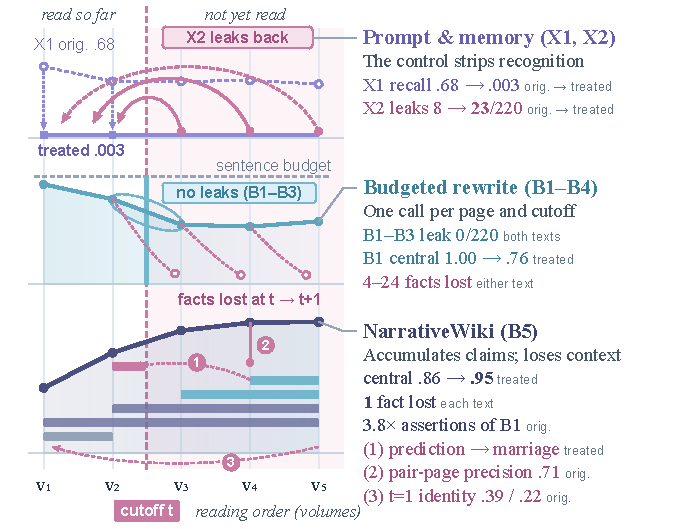
\includegraphics[width=\columnwidth]{figures/teaser-horizon.pdf}
    \caption{Three ways the cutoff behaves over volumes $v_1..v_5$; every number names its
    text (orig.: original; treated: renamed and paraphrased). \textbf{Top:} the control
    removes closed-book recall (X1) and raises disclosures under a cutoff instruction (X2).
    \textbf{Middle:} pages rewritten in one call per cutoff (B1--B3) disclose no assessed
    later fact but lose facts between cutoffs. \textbf{Bottom:} \sys's accumulated claims
    keep central-character recall rising, but lose context: (1) a volume-2 prediction
    printed as the volume-4 marriage, (2) true lines placed on the wrong pair page,
    (3) first-cutoff pages grouped unlike a prefix-built index.}
    \label{fig:teaser}
\end{figure}

A reader consulting a character wiki midway through a series may encounter a later identity,
marriage or death while seeking a reminder of events already read. A reader who has finished
\emph{Anne of Avonlea}, the second book of L.~M.~Montgomery's Anne series, may learn from
Anne Shirley's whole-series page about her marriage to Gilbert Blythe in book four
(Figure~\ref{fig:overview}).\footnote{Examples in this paper reveal plot points of the
series.} A useful reference must respect the reader's progress: at cutoff $t$, every
statement should be established by the first $t$ volumes.

% The overview comes first in the source so that it can take the top of page 2.
\begin{figure*}[t]
\centering
% The teaser has no editable source. f0-teaser-v2.pdf is f0-teaser.pdf with its right-hand
% heading (``Our solution: ...'') and its badge (``No spoilers'') removed from the text layer
% (scripts/papers/redact_teaser_v2.py); both are re-lettered here. Coordinates are fractions
% of the image.
\begin{tikzpicture}
\node[anchor=south west, inner sep=0] (img) at (0,0)
  {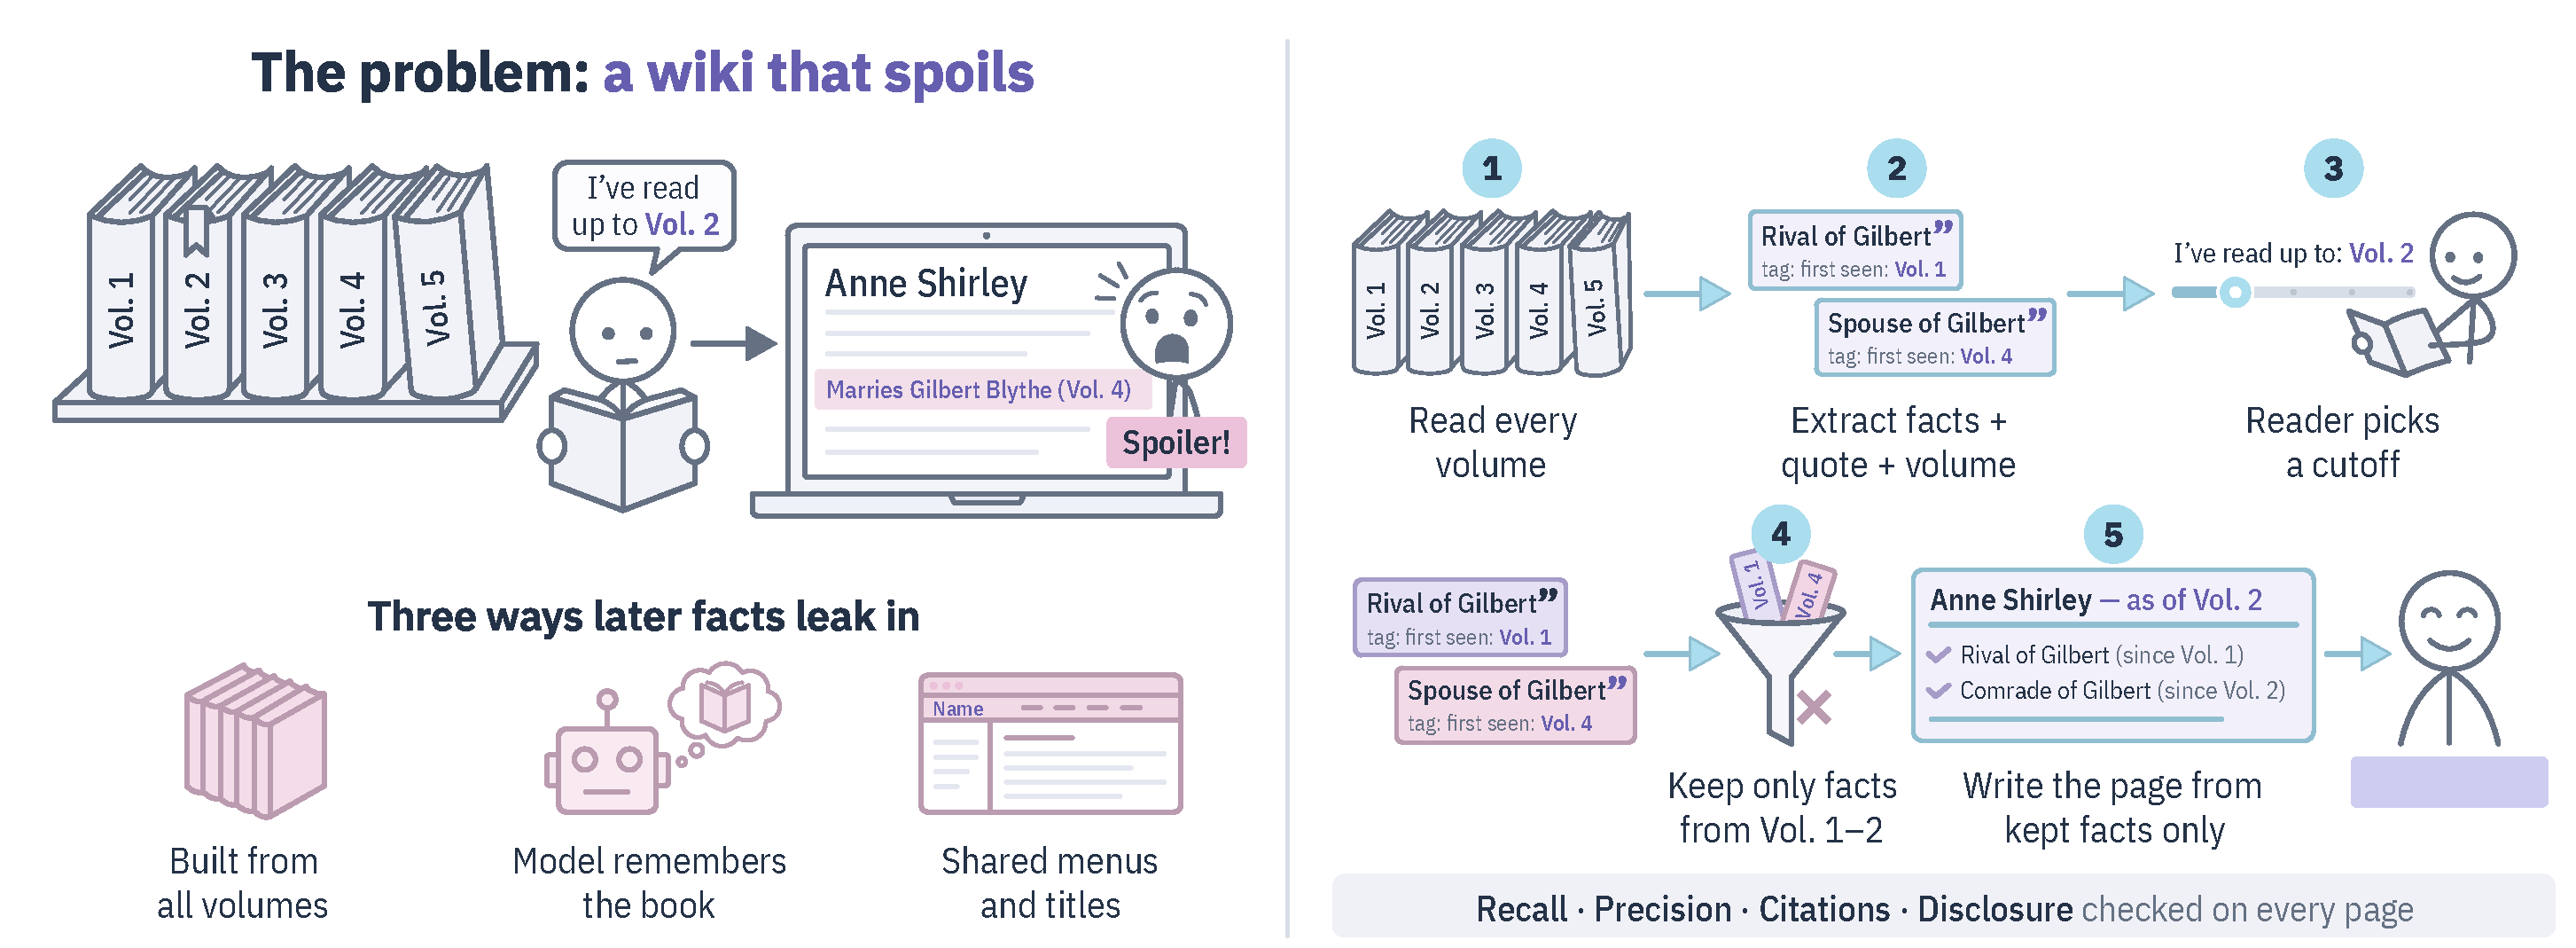
\includegraphics[width=\textwidth]{figures/f0-teaser-v2.pdf}};
\begin{scope}[x={(img.south east)}, y={(img.north west)}]
  \node[font=\sffamily\bfseries\small, text=nwink] at (0.76,0.921)
    {The design under test: \textcolor{nwaccent}{filter, then generate}};
  \node[anchor=north, fill=nwlavender, rounded corners=1pt, inner sep=1.5pt, align=center,
        minimum width=0.08\textwidth, text=nwink,
        font=\sffamily\bfseries\fontsize{5.5}{6}\selectfont] at (0.946,0.207)
    {Cutoff-filtered\\page};
\end{scope}
\end{tikzpicture}
\caption{Overview. Left: a whole-series wiki reveals Anne's marriage to Gilbert (volume~4)
to a reader at volume~2. Later information can enter through a full-series index, generator
memory or surfaces shared across cutoffs. Right: the filter-before-generate design that
\sys implements and this paper probes.}
\label{fig:overview}
\end{figure*}

The natural engineering answer is structural. Decompose the text into a graph of claims,
date each claim by the volume of its evidence, and generate each page from the claims
dated no later than the cutoff, in the manner of graph-based retrieval-augmented generation
\citep{edge2024graphrag,guo2024lightrag}. The boundary is then enforced by data, not by an
instruction to the generator, and one build serves every cutoff. This paper asks what
that decomposition gains and what it costs.

\sys instruments this design as an \emph{analytical probe}, not an advocate: verbatim-evidence
gates, a claim verifier and logged model calls trace each error to its stage, and it is
compared with systems that differ in what the generator sees and how pages are written
(Figure~\ref{fig:systems}).

Such a comparison is interpretable only if scores reflect reading: given only a title and
a character name, the generator recovers \respt{M1-anne-avg-X1} of the eligible gold
facts. We therefore pair every measurement with a \emph{renamed-text control}: a
\emph{treated} copy of the series renames characters and places and paraphrases nearly
every paragraph, keeping paragraph identifiers so that gold facts and citations stay aligned.
Closed-book recall falls to \respt{M1-annedecon-avg-X1}, while systems given text largely
keep theirs (Section~\ref{sec:results-decon}).

Headline means rank \sys below prompting with the text read so far
(Table~\ref{tab:decon}). The probe asks instead \emph{where} decomposition gains and
\emph{where} a volume filter fails, through five research questions on recognition,
cutoff enforcement, accumulation, page context and construction scope (RQ1--RQ5), each
answered in the subsection of Section~\ref{sec:results} with its number
(Table~\ref{tab:glance}).


Prior work bounds dialogue or answers in time \citep{ahn2024timechara,huang2025living}.
We study a linked reference artifact at every cutoff:
\begin{itemize}[leftmargin=*,itemsep=0pt,topsep=2pt]
  \item \textbf{A probe study of structural decomposition} under a reading cutoff,
    separating its gains from failures that a volume filter cannot detect
    (Sections~\ref{sec:method}, \ref{sec:results}).
  \item \textbf{A paired renamed-text control} as evaluation methodology: seven systems
    rebuilt on aligned treated text with unchanged code, prompts and gold facts
    (Section~\ref{sec:results-decon}).
  \item \textbf{A task, threat model and artifact-level protocol} for cutoff-bounded
    reference generation, with \res{T1-anne-gold-t5} gold facts dated by reveal volume
    (Sections~\ref{sec:task}, \ref{sec:setup}; Appendix~\ref{app:corpus}).
\end{itemize}

% Related work (v3). The prior-work matrix is in Appendix~\ref{app:related}.
\section{Related Work}
\label{sec:related}

\paragraph{Spoilers, characters and temporal bounds.}
Spoiler detection labels review sentences without conditioning on a reader's position
\citep{wan2019spoiler}; \citet{jones2018spoilers} serve fan-wiki revisions archived before an
episode aired, and e-readers offer position-bounded answers \citep{amazon2025kindle}, although we are
unaware of a published evaluation. CHIRON builds validated character sheets \citep{gurung2024chiron},
BookWorm pairs books with character descriptions \citep{papoudakis2024bookworm}, and
EvolvTrip graphs characters' mental states over time \citep{yang2025evolvtrip}. TimeChara
measures point-in-time hallucination in role-play \citep{ahn2024timechara}; Living the Novel
gates conversation to the narrative present \citep{huang2025living}, the
filter-before-generate principle we adopt; NS-ST-GraphRAG answers from temporally valid
subgraphs \citep{lin2026nsst}; temporal knowledge graphs attach validity intervals to facts
\citep{dasgupta2018hyte}, ours indexed by reading volume rather than story time. These works
bound answers or dialogue in time; none evaluates a complete linked reference artifact at
every cutoff (Table~\ref{tab:prior}). LitBank annotates identities using the whole text,
including revelations unavailable at an earlier mention \citep{bamman2020litbank}.

\paragraph{Grounded article and wiki generation.}
STORM outlines Wikipedia-like articles \citep{shao2024storm}; GraphRAG summarizes a corpus
entity graph \citep{edge2024graphrag}; LightRAG, a baseline here, combines graph structure with
lightweight retrieval \citep{guo2024lightrag}; SearchWiki builds linked wikis for agents
\citep{singh2026searchwiki}; book-length benchmarks evaluate question answering and
summarization \citep{wang2024novelqa,chang2024booookscore}. Our reference also depends on the
reader's position.

\paragraph{Factuality, attribution and contamination.}
We evaluate atomic support \citep{min2023factscore}, attribution to identified sources
\citep{rashkin2021ais} and citation quality \citep{gao2023alce} across the whole artifact and
in page context. Automatic raters of book-length text can disagree with knowledgeable readers
\citep{kim2024fables}; on STORYSUMM, MiniCheck's Flan-T5 checker \citep{tang2024minicheck}
scored below chance \citep{subbiah2024storysumm}, so we use evidence-reading annotators.
Published novels may be known to the generator \citep{chang2023speak,cheng2025contamination};
renaming entities is an established control \citep{gupta2025whodunit,zhang2024infinitebench},
and rewriting can damage the narrative it protects \citep{sun2025emperor}; we add aligned
paraphrase and audit the treatment.

% Task definition and threat model (v2). Definitions only; no results.
\section{Task and Threat Model}
\label{sec:task}

\paragraph{Cutoffs and the delivered artifact.}
A series comprises ordered volumes $v_1,\dots,v_N$. At cutoff $t$, the reader has read
$\Dt = v_1 \cdots v_t$; the cutoff follows reading order, not story time. The delivered
artifact $\Wt$ includes page text, links and backlinks, titles and addresses, shared
navigation and any search index, group and place pages, and source views opened by
citations. All these surfaces belong to the evaluation scope. Unrequested later information
is in scope; deliberately opening a later cutoff is outside the threat model.

\paragraph{Facts and assertions.}
A gold fact $g$ is a selected character statement with reveal volume $\reveal(g)$, the earliest
volume whose text suffices to establish it. Eligible gold facts are
$\Gt=\{g:\reveal(g)\le t\}$; assessed later facts are
$\Ft=\{g: t<\reveal(g)\le N\}$. The latter are a finite probe set, not an exhaustive spoiler
inventory. Story-level truth, support from eligible text and citation sufficiency are
distinct properties: a true assertion supported only by later text violates the cutoff.
Support must preserve attribution and modality: \emph{A believes B is her father} does
not establish \emph{B is A's father}.

\paragraph{Threats.}
We distinguish three channels.
\emph{Construction dependence}: processing volumes beyond $t$ shapes the early artifact
through alias merges, canonical names or pages created for later characters, even when
rendered claims are filtered.
\emph{Published disclosure}: a delivered surface directly exposes later content, such as
a name in shared navigation.
\emph{Parametric contribution}: the generator supplies memorized information about the work.
An observed disclosure alone cannot identify its channel; experiments therefore vary what
each system can access (Figure~\ref{fig:systems}).

% Method (v2). Stage details, prompts and Algorithm 1 are in Appendix~\ref{app:implementation}.
\section{The Probe: \sys}
\label{sec:method}

\begin{figure*}[t]
\centering
\resizebox{\textwidth}{!}{% F1 (full width): the pipeline on one real example. Every artifact shown is from the frozen Anne
% build: paragraph v01:c15:p0051; the entity anne-shirley; the stored intervals for Anne and
% Gilbert Blythe (ENEMY_OF v1-v1, RIVAL_OF v1-, COMRADE_OF v2-, SPOUSE_OF v4-); the rendered line of
% dist/anne/wiki/v02/relationships/anne-shirley--gilbert-blythe.md. A purple "LLM" tag marks a
% stage that calls the generator; a grey "rule" tag marks a deterministic stage.
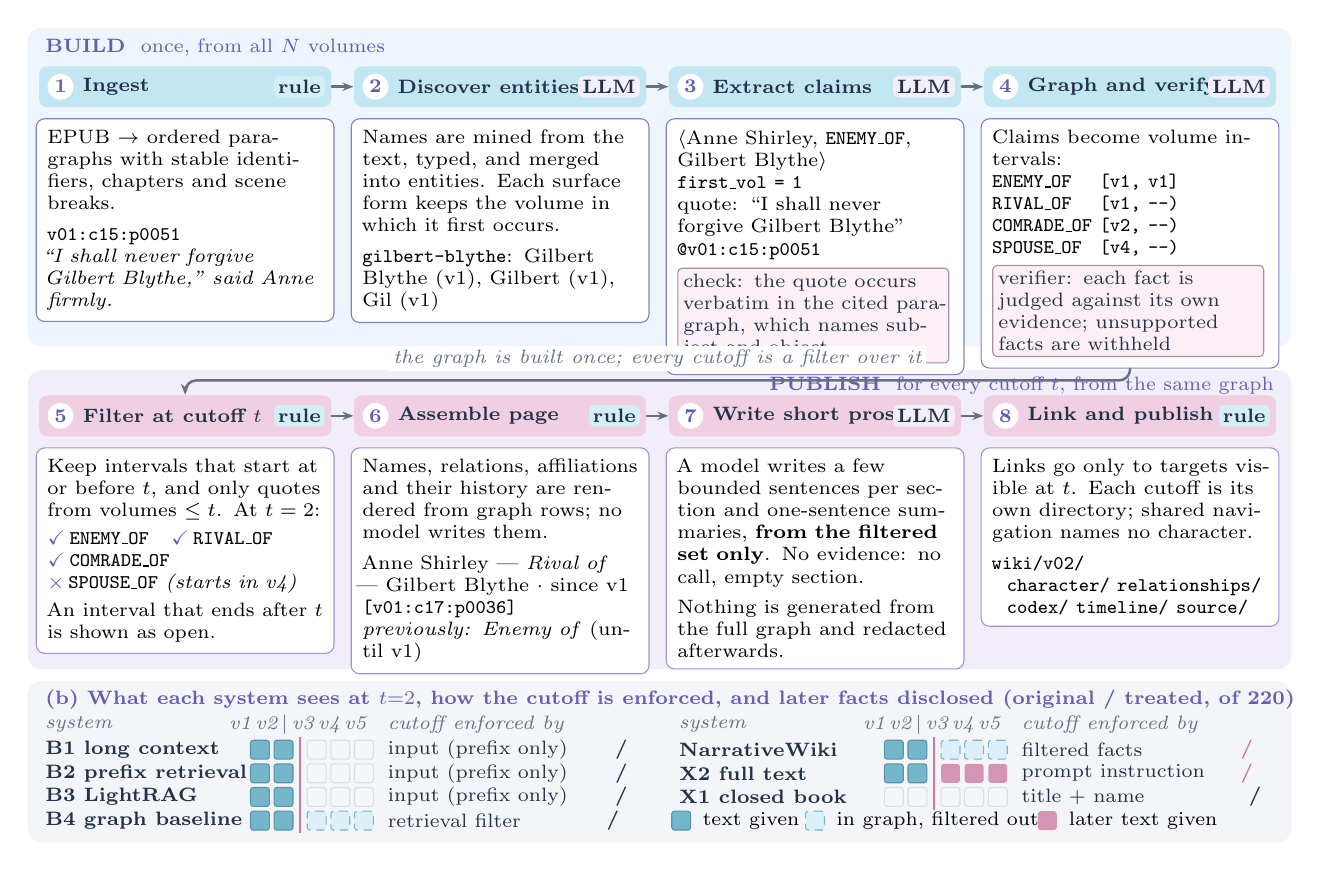
\begin{tikzpicture}[font=\scriptsize,
  head/.style={rounded corners=3pt, minimum height=0.52cm, text width=3.5cm, align=left, inner sep=3pt, font=\scriptsize\bfseries, text=nwink},
  card/.style={draw=#1!75!nwaccent, fill=white, rounded corners=3pt, text width=3.5cm, align=left, inner sep=4pt, font=\figfont, minimum height=1.95cm, anchor=north},
  num/.style={circle, fill=white, text=nwaccent, font=\figfont\bfseries, inner sep=1pt, minimum size=0.33cm},
  tagllm/.style={fill=nwpurplebg, text=nwink, rounded corners=2pt, font=\figfont\bfseries, inner sep=1.5pt},
  tagrule/.style={fill=nwcyan!50, text=nwink, rounded corners=2pt, font=\figfont\bfseries, inner sep=1.5pt},
  gate/.style={fill=nwredbg, draw=nwred!65!nwink, rounded corners=1.5pt, font=\figfont, inner sep=2pt, text=nwink, text width=3.3cm, align=left, minimum height=0pt, anchor=center},
  arr/.style={-{Stealth[length=4pt]}, line width=0.9pt, draw=nwgray,
    rounded corners=4pt, line cap=round, line join=round},
]
\def\dx{4.0}
% ---------------- phase bands
\begin{scope}[on background layer]
  \fill[nwbluebg, rounded corners=5pt] (-2.0,0.75) rectangle (14.05,-3.3);
  \fill[nwgreenbg, rounded corners=5pt] (-2.0,-3.6) rectangle (14.05,-7.4);
\end{scope}
\node[anchor=west, font=\scriptsize\bfseries, text=nwaccent] at (-1.9,0.5) {BUILD \;\textnormal{once, from all $N$ volumes}};
\node[anchor=east, font=\scriptsize\bfseries, text=nwaccent] at (13.95,-3.8) {PUBLISH \;\textnormal{for every cutoff $t$, from the same graph}};
% ---------------- row 1: build
\foreach \i/\t/\tag/\lbl in {0/Ingest/rule/rule, 1/Discover entities/llm/LLM, 2/Extract claims/llm/LLM, 3/Graph and verify/llm/LLM}{
  \pgfmathtruncatemacro{\n}{\i+1}
  \node[head, fill=nwcyan!72] (h\n) at (\i*\dx,0) {\hspace{0.45cm}\t};
  \node[num=nwblue] at ($(h\n.west)+(0.28,0)$) {\n};
  \node[tag\tag, anchor=east] at ($(h\n.east)+(-0.08,0)$) {\lbl};
}
\node[card=nwblue] (c1) at (0*\dx,-0.4) {%
  EPUB $\rightarrow$ ordered paragraphs with stable identifiers, chapters and scene breaks.\\[3pt]
  {\ttfamily v01:c15:p0051}\\
  \emph{``I shall never forgive Gilbert Blythe,'' said Anne firmly.}};
\node[card=nwblue] (c2) at (1*\dx,-0.4) {%
  Names are mined from the text, typed, and merged into entities. Each surface form keeps the volume in which it first occurs.\\[3pt]
  {\ttfamily gilbert-blythe}: Gilbert Blythe (v1), Gilbert (v1), Gil (v1)};
\node[card=nwblue] (c3) at (2*\dx,-0.4) {%
  $\langle$Anne Shirley, {\ttfamily ENEMY\_OF}, Gilbert Blythe$\rangle$\\
  {\ttfamily first\_vol = 1}\\
  quote: ``I shall never forgive Gilbert Blythe'' {\ttfamily @v01:c15:p0051}\\[2pt]
  \tikz[baseline=-2pt]\node[gate]{check: the quote occurs verbatim in the cited paragraph, which names subject and object};};
\node[card=nwblue] (c4) at (3*\dx,-0.4) {%
  Claims become volume intervals:\\
  {\ttfamily ENEMY\_OF\phantom{xx} [v1, v1]}\\
  {\ttfamily RIVAL\_OF\phantom{xx} [v1, --)}\\
  {\ttfamily COMRADE\_OF [v2, --)}\\
  {\ttfamily SPOUSE\_OF\phantom{x} [v4, --)}\\[2pt]
  \tikz[baseline=-2pt]\node[gate]{verifier: each fact is judged against its own evidence; unsupported facts are withheld};};
% ---------------- row 2: publish
\foreach \i/\t/\tag/\lbl in {0/Filter at cutoff $t$/rule/rule, 1/Assemble page/rule/rule, 2/Write short prose/llm/LLM, 3/Link and publish/rule/rule}{
  \pgfmathtruncatemacro{\n}{\i+5}
  \node[head, fill=nwred!78] (h\n) at (\i*\dx,-4.18) {\hspace{0.45cm}\t};
  \node[num=nwgreen] at ($(h\n.west)+(0.28,0)$) {\n};
  \node[tag\tag, anchor=east] at ($(h\n.east)+(-0.08,0)$) {\lbl};
}
\node[card=nwgreen] (c5) at (0*\dx,-4.58) {%
  Keep intervals that start at or before $t$, and only quotes from volumes $\le t$. At $t=2$:\\[2pt]
  {\color{nwaccent}\checkmark}\,{\ttfamily ENEMY\_OF}\quad{\color{nwaccent}\checkmark}\,{\ttfamily RIVAL\_OF}\\
  {\color{nwaccent}\checkmark}\,{\ttfamily COMRADE\_OF}\\
  {\color{nwaccent}$\times$}\,{\ttfamily SPOUSE\_OF} \emph{(starts in v4)}\\[2pt]
  An interval that ends after $t$ is shown as open.};
\node[card=nwgreen] (c6) at (1*\dx,-4.58) {%
  Names, relations, affiliations and their history are rendered from graph rows; no model writes them.\\[3pt]
  Anne Shirley --- \emph{Rival of} --- Gilbert Blythe $\cdot$ since v1 {\ttfamily [v01:c17:p0036]}\\
  \emph{previously: Enemy of} (until v1)};
\node[card=nwgreen] (c7) at (2*\dx,-4.58) {%
  A model writes a few bounded sentences per section and one-sentence summaries, \textbf{from the filtered set only}. No evidence: no call, empty section.\\[3pt]
  Nothing is generated from the full graph and redacted afterwards.};
\node[card=nwgreen] (c8) at (3*\dx,-4.58) {%
  Links go only to targets visible at $t$. Each cutoff is its own directory; shared navigation names no character.\\[3pt]
  {\ttfamily wiki/v02/}\\
  {\ttfamily \ \ character/ relationships/}\\
  {\ttfamily \ \ codex/ timeline/ source/}};
% ---------------- arrows
\foreach \a/\b in {1/2,2/3,3/4,5/6,6/7,7/8}{ \draw[arr] (h\a.east) -- (h\b.west); }
\draw[arr] (c4.south) -- ++(0,-0.15) -| (h5.north);
\node[font=\figfont\itshape, text=nwgray, fill=white, inner sep=1.5pt] at (6.0,-3.45) {the graph is built once; every cutoff is a filter over it};
% ---------------- (b) v4: the experimental matrix at t=2 (was the separate Figure fig:systems).
% Counts are later facts stated or implied, original / treated text (Table tab:decon).
\begin{scope}[shift={(0,-7.6)},
  cell/.style={minimum width=0.24cm, minimum height=0.24cm, inner sep=0pt, rounded corners=1pt},
  seen/.style={cell, fill=nwCyan, draw=nwCyan!80!black},
  later/.style={cell, fill=nwMagenta!80},
  built/.style={cell, fill=nwhighcyan, draw=nwCyan, densely dashed},
  none/.style={cell, draw=nwLight, fill=nwgraybg},
  sysn/.style={anchor=west, font=\figfont\bfseries, text=nwink},
  how/.style={anchor=west, font=\figfont, text=nwink},
  cnt/.style={anchor=east, font=\figfont\bfseries, text=nwink}]
\fill[nwgraybg, rounded corners=5pt] (-2.0,0.05) rectangle (14.05,-2.0);
\node[anchor=west, font=\scriptsize\bfseries, text=nwaccent] at (-1.9,-0.18)
  {(b) What each system sees at $t{=}2$, how the cutoff is enforced, and later facts disclosed (original / treated, of 220)};
% \mrow{x}{y}{name}{v1..v5 styles}{how}{counts}
\newcommand{\mrow}[9]{%
  \node[sysn] at (#1,#2) {#3};
  \foreach \k/\s in {1/#4,2/#5,3/#6,4/#7,5/#8}{\node[\s] at ({#1+2.55+\k*0.3+(\k>2)*0.12},#2) {};}
  \draw[nwMagenta, line width=0.8pt] (#1+3.36,#2+0.16) -- (#1+3.36,#2-0.16);
  \node[how] at (#1+4.35,#2) {#9};}
\newcommand{\mcnt}[3]{\node[cnt] at (#1,#2) {#3};}
\foreach \x in {-1.9, 6.15}{
  \node[anchor=west, font=\figfont\itshape, text=nwgray] at (\x,-0.5) {system};
  \node[font=\figfont\itshape, text=nwgray] at (\x+3.33,-0.5) {v1\,v2\,$|$\,v3\,v4\,v5};
  \node[anchor=west, font=\figfont\itshape, text=nwgray] at (\x+4.35,-0.5) {cutoff enforced by};}
\mrow{-1.9}{-0.82}{B1 long context}{seen}{seen}{none}{none}{none}{input (prefix only)}
\mrow{-1.9}{-1.12}{B2 prefix retrieval}{seen}{seen}{none}{none}{none}{input (prefix only)}
\mrow{-1.9}{-1.42}{B3 LightRAG}{seen}{seen}{none}{none}{none}{input (prefix only)}
\mrow{-1.9}{-1.72}{B4 graph baseline}{seen}{seen}{built}{built}{built}{retrieval filter}
\mcnt{5.85}{-0.82}{\respt{M4-anne-total-B1} / \respt{M4-annedecon-total-B1}}
\mcnt{5.85}{-1.12}{\respt{M4-anne-total-B2} / \respt{M4-annedecon-total-B2}}
\mcnt{5.85}{-1.42}{\respt{M4-anne-total-B3} / \respt{M4-annedecon-total-B3}}
\mcnt{5.85}{-1.72}{\respt{M4-anne-total-B4} / \textcolor{nwMagenta}{\respt{M4-annedecon-total-B4}}}
\mcnt{13.9}{-0.82}{\textcolor{nwMagenta}{\respt{M4-anne-total-B5} / \respt{M4-annedecon-total-B5}}}
\mcnt{13.9}{-1.12}{\textcolor{nwMagenta}{\respt{M4-anne-total-X2} / \respt{M4-annedecon-total-X2}}}
\mcnt{13.9}{-1.42}{\textcolor{nwMagenta}{\respt{M4-anne-total-X1}} / \respt{M4-annedecon-total-X1}}
\mrow{6.15}{-0.82}{\sys}{seen}{seen}{built}{built}{built}{filtered facts}
\mrow{6.15}{-1.12}{X2 full text}{seen}{seen}{later}{later}{later}{prompt instruction}
\mrow{6.15}{-1.42}{X1 closed book}{none}{none}{none}{none}{none}{title + name}
\node[seen] at (6.3,-1.72) {}; \node[anchor=west, font=\figfont] at (6.45,-1.72) {text given};
\node[built] at (8.0,-1.72) {}; \node[anchor=west, font=\figfont] at (8.15,-1.72) {in graph, filtered out};
\node[later] at (10.95,-1.72) {}; \node[anchor=west, font=\figfont] at (11.1,-1.72) {later text given};
\end{scope}
\end{tikzpicture}
}
\caption{The \sys pipeline on a stored fact. \textsc{Build} converts all volumes into
identified paragraphs, entities and claim intervals accepted by the verifier. \textsc{Publish} assembles
each cutoff's wiki from eligible intervals and quotes. Stages marked \textsc{llm} call the
generator; other stages are deterministic. Validation gates check verbatim evidence and
fact-level support. (b) The experimental matrix: what each system can see at cutoff~2, how
it enforces the cutoff, and the assessed later facts it disclosed over $t=1..4$ on the
original and the treated text. X1 and X2 are diagnostics.}
\label{fig:pipeline}\label{fig:systems}
\end{figure*}

\sys constructs a graph of evidence-bearing claims with volume intervals and renders one
wiki per cutoff (Figure~\ref{fig:pipeline}). Claims are filtered to evidence volumes $\le t$
before page assembly and prose generation. Filtering precedes generation because removing
explicit later facts from generated text can leave implications intact.

\paragraph{Ingestion and entities (stages 1--2).}
Volumes become ordered paragraphs with stable citation identifiers such as
\pid{v01:c06:p0003}. Lexical mining identifies capitalized n-grams, honorifics and vocatives;
the model types them as characters, groups, places, events or objects. Surface forms are
clustered by exact match, fuzzy match and whole-word subset, followed by model adjudication
of ambiguous pairs using passages containing both names. A bare name is not automatically
merged with a fuller name first appearing later. Shared first names are assigned
volume by volume to the locally dominant full name. Entities use the fullest title occurring
in their first volume, and surface forms retain their first-occurrence volume.

\paragraph{Claims with evidence (stage 3).}
Three extraction passes share a schema: subject, predicate, object or value, qualifier,
first-evidence volume (\firstvol), verbatim quotes and paragraph identifiers.
A chapter pass covers every paragraph in overlapping spans and extracts scenes, participants
and summaries backed by up to four paragraphs. A mention pass reads windows around each
character's mentions; a long-context pass reads all their paragraphs in a volume for
attributes and background. Claims are retained only when the quote occurs verbatim in its
cited paragraph, the subject is named in or beside that paragraph (and, for twelve
two-person relations, the object in it), and relation objects resolve to known entities.

\paragraph{Intervals and verification (stage 4).}
Claims become volume intervals. Conflicting values of a single-valued attribute within one
volume are arbitrated as extraction conflicts; values in different volumes are treated as
story changes, closing the earlier interval when the later one opens. Near-duplicate values
are clustered with BGE-M3 embeddings \citep{chen2024m3}. A verifier judges each assembled
fact against its cited evidence in a separate call; rejected facts (\res{VERIFY-unsupported}
checked) are withheld.
On \res{M12-n} constructed minimal-edit items the verifier reaches \res{M12-verifier-bacc}
balanced accuracy (MiniCheck: \res{M12-mc-bacc}), and \res{OBS-hard-verifier-bacc} on
\res{OBS-hard-items} harder items of embedded speech (Appendix~\ref{app:evaluator}).

\paragraph{Cutoff assembly and publication (stages 5--8).}
Deterministic assembly selects intervals opening by $t$
(Algorithm~\ref{alg:assemble}, Appendix~\ref{app:implementation}). Each quote is filtered
by its own volume; intervals closing after $t$ appear current to conceal future changes;
and qualifiers must be supported no later than the interval's start. Names, attributes,
affiliations and relations are rendered directly from graph rows. The model writes only
short prose from filtered facts, with sentence limits per section
(Appendix~\ref{app:implementation}), and is instructed to identify the input lines supporting it.
Line keys select source paragraphs; returned paragraph IDs are normalized during citation
resolution. Sections without evidence remain empty without a model call.
String matching adds links using surface forms revealed by $t$. Cutoffs occupy separate
directories, shared navigation names no characters, and no site-wide search index is shipped
because it would span cutoffs.

\paragraph{Build scope.}
One graph is built from all volumes. Additional cutoffs require no extraction, structured
content is rendered without model calls, and prose is generated once per distinct eligible
fact set. This efficiency retains construction dependence (Section~\ref{sec:task}), which
we assess against prefix-only builds (Section~\ref{sec:results-scope}). Every model stage,
including verification, uses the generator specified in Section~\ref{sec:setup}.

% Experimental setup (v2). Every number is a \res key.
\section{Experimental Setup}
\label{sec:setup}

\paragraph{Corpus and gold facts.}
We evaluate the first five novels in publication order of L.~M.~Montgomery's Anne series,
from \emph{Anne of Green Gables} to \emph{Rainbow Valley}, using Project Gutenberg editions:
\res{T1-anne-words} words, \res{T1-anne-paras} paragraphs and \res{T1-anne-chapters} chapters
(Appendix~\ref{app:corpus}).
The gold inventory contains \res{T1-anne-gold-t5} facts about \res{T1-anne-cast} characters,
each with a reveal volume and an evidence paragraph. It was drafted from the source text
without access to system outputs; eligible counts at each cutoff appear in
Table~\ref{tab:corpus}.
\ifnwhuman For 85 of the \res{T1-anne-gold-t5} facts the cited paragraph suffices alone;
the other 26 (23 established in part, three not) need text beyond that paragraph and
are retained unchanged (Appendix~\ref{app:annotation}).\fi{}
Recall measures coverage of this selected inventory rather than all facts in the novels.

\paragraph{Systems.}
All systems use \res{GEN-model}. Comparison systems share a character-page template,
requested sentence limits and citation format. A cast character receives a page at $t$ if an eligible
gold fact concerns them or their full name occurs in $\Dt$
(\res{PAGES-anne-cast} pages at $t=1..5$; Table~\ref{tab:artifact-size}).
\textbf{B1} (long context) supplies the complete prefix $\Dt$ to the generator.
\textbf{B2} (prefix retrieval) combines BM25 and dense retrieval from a prefix-only index.
\textbf{B3} uses prefix-built LightRAG \citep{guo2024lightrag} as the shared generator's retriever.
\textbf{B4}, the graph baseline, retrieves from the full five-volume \sys graph, filtering
facts at retrieval time; it controls for the graph while changing page generation and
publication scope.
\textbf{B5} is \sys: it discovers its own entities and also publishes other character,
relationship, codex and timeline pages. We evaluate its full artifact and separately examine
the cast character pages shared with the baselines.
\textbf{X1} receives only the title and character name (closed book).
\textbf{X2} receives all five volumes with an instruction to reveal nothing after $t$.
These two diagnostics are excluded from best-system comparisons. Baseline settings were
fixed on a separate development novel (Appendix~\ref{app:baselines}).

% Master results table (v3): the former Table 1 (treated beside original) merged with the former
% Table 11 (original summary, distinct assertions, tokens). Original-text standard deviations are
% in Table tab:stats. Both labels point here so earlier references resolve.
\begin{table*}[tp]
\centering\footnotesize
\setlength{\tabcolsep}{2pt}
\resizebox{\textwidth}{!}{%
\begin{tabular}{@{}llccccccccccc@{}}
\toprule
 &  & \multicolumn{3}{c}{\nwhead{Recall $\uparrow$}} & \multicolumn{2}{c}{\nwhead{Precision $\uparrow$}} & \multicolumn{2}{c}{\nwhead{Citation suff.\ $\uparrow$}} & \multicolumn{2}{c}{\nwhead{Later facts /220 $\downarrow$}} & \nwhead{Distinct} & \nwhead{Tokens} \\
\cmidrule(lr){3-5}\cmidrule(lr){6-7}\cmidrule(lr){8-9}\cmidrule(lr){10-11}
\multicolumn{2}{@{}l}{\nwhead{System}} & \nwhead{treated} & \nwhead{orig.} & \nwhead{diff.} & \nwhead{treated} & \nwhead{orig.} & \nwhead{treated} & \nwhead{orig.} & \nwhead{orig.} & \nwhead{treated} & \nwhead{assertions} & \nwhead{in / out (M)} \\
\midrule
B1 & Long context & \cellcolor{nwhighcyan}\best{\res{M1-annedecon-avg-B1}}\sdev{\res{M1-annedecon-sd-B1}} & \cellcolor{nwhighcyan}\best{\respt{M1-anne-avg-B1}} & \res{M1-annedecon-diff-B1} & \res{M3-annedecon-avg-B1}\sdev{\res{M3-annedecon-sd-B1}} & \respt{M3-anne-avg-B1} & \res{M8-annedecon-avg-B1}\sdev{\res{M8-annedecon-sd-B1}} & \respt{M8-anne-avg-B1} & \cellcolor{nwhighcyan}\respt{M4-anne-total-B1} & \cellcolor{nwhighcyan}\respt{M4-annedecon-total-B1} & \res{ND-anne-avg-B1} & \res{TOK-anne-B1} \\
B2 & Prefix retrieval & \res{M1-annedecon-avg-B2}\sdev{\res{M1-annedecon-sd-B2}} & \respt{M1-anne-avg-B2} & \res{M1-annedecon-diff-B2} & \res{M3-annedecon-avg-B2}\sdev{\res{M3-annedecon-sd-B2}} & \respt{M3-anne-avg-B2} & \res{M8-annedecon-avg-B2}\sdev{\res{M8-annedecon-sd-B2}} & \respt{M8-anne-avg-B2} & \cellcolor{nwhighcyan}\respt{M4-anne-total-B2} & \cellcolor{nwhighcyan}\respt{M4-annedecon-total-B2} & \res{ND-anne-avg-B2} & \cellcolor{nwhighviolet}\best{\res{TOK-anne-B2}} \\
B3 & LightRAG & \res{M1-annedecon-avg-B3}\sdev{\res{M1-annedecon-sd-B3}} & \respt{M1-anne-avg-B3} & \res{M1-annedecon-diff-B3} & \cellcolor{nwhighcyan}\best{\res{M3-annedecon-avg-B3}}\sdev{\res{M3-annedecon-sd-B3}} & \respt{M3-anne-avg-B3} & \res{M8-annedecon-avg-B3}\sdev{\res{M8-annedecon-sd-B3}} & \respt{M8-anne-avg-B3} & \cellcolor{nwhighcyan}\respt{M4-anne-total-B3} & \cellcolor{nwhighcyan}\respt{M4-annedecon-total-B3} & \res{ND-anne-avg-B3} & \res{TOK-anne-B3} \\
B4 & Graph baseline & \res{M1-annedecon-avg-B4}\sdev{\res{M1-annedecon-sd-B4}} & \respt{M1-anne-avg-B4} & \res{M1-annedecon-diff-B4} & \res{M3-annedecon-avg-B4}\sdev{\res{M3-annedecon-sd-B4}} & \cellcolor{nwhighcyan}\best{\respt{M3-anne-avg-B4}} & \cellcolor{nwhighcyan}\best{\res{M8-annedecon-avg-B4}}\sdev{\res{M8-annedecon-sd-B4}} & \cellcolor{nwhighcyan}\best{\respt{M8-anne-avg-B4}} & \respt{M4-anne-total-B4} & \cellcolor{nwhighpink}\best{\respt{M4-annedecon-total-B4}} & \res{ND-anne-avg-B4} & +\res{TOK-anne-B4} \\
B5 & \sys & \res{M1-annedecon-avg-B5}\sdev{\res{M1-annedecon-sd-B5}} & \respt{M1-anne-avg-B5} & \cellcolor{nwhighviolet}\best{\res{M1-annedecon-diff-B5}} & \res{M3-annedecon-avg-B5}\sdev{\res{M3-annedecon-sd-B5}} & \respt{M3-anne-avg-B5} & \res{M8-annedecon-avg-B5}\sdev{\res{M8-annedecon-sd-B5}} & \respt{M8-anne-avg-B5} & \cellcolor{nwhighpink}\best{\respt{M4-anne-total-B5}} & \cellcolor{nwhighpink}\best{\respt{M4-annedecon-total-B5}} & \cellcolor{nwhighviolet}\best{\res{ND-anne-avg-B5}} & \res{TOK-anne-B5} \\
\midrule
X1 & Closed book & \res{M1-annedecon-avg-X1}\sdev{\res{M1-annedecon-sd-X1}} & \respt{M1-anne-avg-X1} & \cellcolor{nwhighpink}\best{\res{M1-annedecon-diff-X1}} & \res{M3-annedecon-avg-X1}\sdev{\res{M3-annedecon-sd-X1}} & \respt{M3-anne-avg-X1} & -- & -- & \cellcolor{nwhighpink}\best{\respt{M4-anne-total-X1}} & \respt{M4-annedecon-total-X1} & \res{ND-anne-avg-X1} & \res{TOK-anne-X1} \\
X2 & Full text & \res{M1-annedecon-avg-X2}\sdev{\res{M1-annedecon-sd-X2}} & \respt{M1-anne-avg-X2} & \res{M1-annedecon-diff-X2} & \res{M3-annedecon-avg-X2}\sdev{\res{M3-annedecon-sd-X2}} & \respt{M3-anne-avg-X2} & \res{M8-annedecon-avg-X2}\sdev{\res{M8-annedecon-sd-X2}} & \respt{M8-anne-avg-X2} & \cellcolor{nwhighpink}\best{\respt{M4-anne-total-X2}} & \cellcolor{nwhighpink}\best{\respt{M4-annedecon-total-X2}} & \res{ND-anne-avg-X2} & \res{TOK-anne-X2} \\
\bottomrule
\end{tabular}}
\caption{Main results on the original and the treated text (renamed, paraphrased), with
unchanged code, prompts and gold facts. Rates: unweighted means over $t=1..5$, treated rates
$\pm$ sample SD (original: Table~\ref{tab:stats}). Diff.: treated minus original. Later
facts: stated or implied disclosures of 220 fact--cutoff pairs, $t=1..4$. Distinct
assertions: mean per cutoff, original text; tokens: all cutoffs (B4: added to \sys's build).
X1, X2: diagnostics. Cell colours in every table: cyan, best; magenta, failure, disclosure
or worst; violet or lavender, size, cost or inventory.}
\label{tab:decon}
\end{table*}
% declared here so the float lands on the first Results page
\paragraph{Paired text conditions.}
Every system is built twice, on the original and on the treated text
(Appendix~\ref{app:contamination}). A reviewed map of \res{DECON-map} entries renames
characters, families and local places, and the generator paraphrases each renamed
paragraph, preserving facts, order and speakers. Paragraph identifiers and the mapped gold
facts carry over, so rules, code and prompts are unchanged.

\paragraph{Metrics.}
We report four separate outcomes (Figure~\ref{fig:protocol}; Appendix~\ref{app:annotation}).
\emph{Recall} is the fraction of eligible gold facts stated of the correct character
anywhere in $\Wt$.
\emph{Precision} measures full support in $\Dt$ for 40 uniformly sampled atomic
assertions per system and cutoff, drawn from an inventory of all delivered surfaces
\citep{min2023factscore}. Assertions are judged in their page context: a true scene line
on a relationship page is supported there only if both characters participate in a shared
episode of that scene (the \emph{scene rule}); we also record whether each assertion is true
as a statement. \emph{Citation sufficiency} is the fraction of sampled assertions fully established
by their cited paragraphs alone; uncited assertions count as insufficient.
\emph{Disclosure} searches every page for every assessed later fact using three
lexical routes. Retrieved candidates are labeled \emph{stated}, \emph{implied},
\emph{uncertain} or absent; stated and implied count as disclosure. There are 220
fact--cutoff assessments per system at $t=1..4$; disclosure is undefined at $t=5$.
We measure the candidate search's recall on seeded disclosures and add two complementary
checks that do not use it: later-only support among sampled assertions, and names in $\Wt$ that
occur in the full entity index but not in $\Dt$.

\paragraph{Annotation.}
Labels come from LLM coding agents that read the evidence under written rules
(Appendix~\ref{app:annotation}): OpenAI Codex and Claude Opus~5.5 produced first-pass labels,
and Claude Opus~5.5 finalized every reported label, including the gold facts. The pair
verdict is the judgment that moves precision most: first-pass and final verdicts agree on
\res{ANN-pair-agree} (Cohen's $\kappa=\res{ANN-pair-kappa}$), and the first-pass verdicts
would give \sys a precision of \res{REV-M3-pair2} instead of \respt{M3-anne-avg-B5}.
Reported values incorporate consistency audits\ifnwhuman{} and a review-triggered recall
recheck\fi{} (Appendix~\ref{app:annotation}).
\ifnwhuman Two human reviewers independently relabeled \res{HREV-total} original-text
items, all gold facts and 10\% samples of the recall, precision and citation labels,
without seeing the AI answers ($\kappa$ from \res{HREV-P-kappa-2dp} on precision to
\res{HREV-R-kappa-2dp} on recall; Table~\ref{tab:human-agreement}).\fi{}

\paragraph{Statistics.}
Means are unweighted over cutoffs; each cell is built once, so standard deviations
describe variation across cutoffs (medians, ranges, paired differences:
Tables~\ref{tab:stats},~\ref{tab:paired}).

% Results (v3): one subsection per research question, with declarative headings. Subsection labels
% are those of v2, which the appendices reference. Every number is a \res key.
\section{Results}
\label{sec:results}
% tables/t2b-decon is declared in sections/05-setup.tex for float placement.

\begin{figure*}[t]
\centering
\resizebox{\textwidth}{!}{% F6 (v3, full width): the renamed-and-paraphrased control in one view (RQ1/RQ2). Vector redraw of
% the dashboard proposed in the 2026-10-18 review, with the system names corrected. Plotted
% coordinates are typed from results.tex keys and must be re-typed if they change:
% (a) MEM-title-*, MEM-author-*, MEM-cloze-*; (b) M1-anne-avg-*, M1-annedecon-avg-*;
% (c) M4-anne-total-*, M4-annedecon-total-*; (d) M8-anne-t*-B1, M8-annedecon-t*-B1, M8-annedecon-t*-B4.
% Printed labels are \res keys wherever the value is printed.
\begin{tikzpicture}[x=1cm, y=0.82cm, font=\figfont,
  ptitle/.style={anchor=north west, font=\figfont\bfseries, text=nwink, inner sep=0pt},
  tick/.style={font=\fontsize{5.6}{6}\selectfont, text=nwSlate},
  val/.style={font=\fontsize{5.4}{6}\selectfont, text=nwink, inner sep=1pt}]
\def\Hh{2.5}

% ------------------------------------------------------------- (a) recognition
\begin{scope}[shift={(0,0)}]
\node[ptitle] at (-0.2,3.35) {(a) Recognition, 200 paragraphs};
\foreach \v/\l in {0/0, 0.5/0.5, 1/1.0}{\draw[nwgrid] (0,\v*\Hh) -- (3.45,\v*\Hh); \node[tick, anchor=east] at (0,\v*\Hh) {\l};}
% bars: \bar{x}{value}{colour}
\newcommand{\rbar}[3]{\fill[#3] (#1,0) rectangle (#1+0.26,#2*\Hh); \node[val, anchor=south] at (#1+0.13,#2*\Hh) {\rotatebox{90}{#2}};}
\rbar{0.15}{0.820}{nwMid}\rbar{0.43}{0.325}{nwLav}\rbar{0.71}{0.110}{nwCyan}
\rbar{1.30}{0.865}{nwMid}\rbar{1.58}{0.625}{nwLav}\rbar{1.86}{0.195}{nwCyan}
\rbar{2.60}{0.165}{nwMid}\rbar{2.88}{0.000}{nwCyan}
\node[tick] at (0.56,-0.2) {title}; \node[tick] at (1.71,-0.2) {author}; \node[tick] at (2.87,-0.2) {name cloze};
\fill[nwMid] (0.05,-0.52) rectangle (0.2,-0.42); \node[tick, anchor=west] at (0.2,-0.47) {original};
\fill[nwLav] (1.05,-0.52) rectangle (1.2,-0.42); \node[tick, anchor=west] at (1.2,-0.47) {renamed};
\fill[nwCyan] (2.05,-0.52) rectangle (2.2,-0.42); \node[tick, anchor=west] at (2.2,-0.47) {+ paraphrase};
\end{scope}

% ------------------------------------------------------------- (b) recall, original vs treated
\begin{scope}[shift={(4.25,0)}]
\node[ptitle] at (-0.95,3.35) {(b) Gold recall, mean over $t$};
\def\W{2.6}
\foreach \v/\l in {0/0, 0.5/0.5, 1/1.0}{\draw[nwgrid] (\v*\W,-0.05) -- (\v*\W,2.85); \node[tick] at (\v*\W,-0.2) {\l};}
% \dumb{y}{name}{orig}{treated}{colour}{change}
\newcommand{\dumb}[6]{\node[tick, anchor=east, text=nwink] at (-0.05,#1) {#2};
  \draw[nwMid, line width=0.6pt] (#3*\W,#1) -- (#4*\W,#1);
  \draw[nwSlate, fill=white, line width=0.45pt] (#3*\W,#1) circle (1.6pt);
  \fill[#5] (#4*\W,#1) circle (1.6pt);
  \node[tick, anchor=west, text=#5!80!black] at (\W+0.05,#1) {#6};}
\dumb{2.7}{B1}{0.848}{0.845}{nwSlate}{\res{M1-annedecon-diff-B1}}
\dumb{2.3}{B2}{0.834}{0.784}{nwSlate}{\res{M1-annedecon-diff-B2}}
\dumb{1.9}{B3}{0.536}{0.470}{nwSlate}{\res{M1-annedecon-diff-B3}}
\dumb{1.5}{B4}{0.761}{0.704}{nwSlate}{\res{M1-annedecon-diff-B4}}
\dumb{1.1}{B5}{0.802}{0.843}{nwCyan}{\res{M1-annedecon-diff-B5}}
\dumb{0.6}{X2}{0.814}{0.744}{nwSlate}{\res{M1-annedecon-diff-X2}}
\dumb{0.2}{X1}{0.683}{0.003}{nwMagenta}{\res{M1-annedecon-diff-X1}}
\draw[nwSlate, fill=white, line width=0.45pt] (0.0,-0.47) circle (1.6pt); \node[tick, anchor=west] at (0.08,-0.47) {original};
\fill[nwSlate] (1.2,-0.47) circle (1.6pt); \node[tick, anchor=west] at (1.28,-0.47) {treated};
\end{scope}

% ------------------------------------------------------------- (c) later facts disclosed
\begin{scope}[shift={(9.05,0)}]
\node[ptitle] at (-0.6,3.35) {(c) Later facts disclosed / 220};
\def\Sc{0.105}
\foreach \v in {0,10,20}{\draw[nwgrid] (\v*\Sc,-0.05) -- (\v*\Sc,2.85); \node[tick] at (\v*\Sc,-0.2) {\v};}
% \disc{y}{name}{orig}{treated}
\newcommand{\disc}[4]{\node[tick, anchor=east, text=nwink] at (-0.05,#1) {#2};
  \fill[nwMid] (0,#1+0.02) rectangle (#3*\Sc+0.001,#1+0.17); \node[val, anchor=west] at (#3*\Sc,#1+0.095) {#3};
  \fill[nwMagenta] (0,#1-0.17) rectangle (#4*\Sc+0.001,#1-0.02); \node[val, anchor=west] at (#4*\Sc,#1-0.095) {#4};}
\disc{2.55}{B1--B3}{0}{0}
\disc{2.0}{B4}{0}{2}
\disc{1.45}{B5}{1}{4}
\disc{0.9}{X1}{4}{0}
\disc{0.35}{X2}{8}{23}
\fill[nwMid] (0.0,-0.52) rectangle (0.15,-0.42); \node[tick, anchor=west] at (0.15,-0.47) {original};
\fill[nwMagenta] (1.1,-0.52) rectangle (1.25,-0.42); \node[tick, anchor=west] at (1.25,-0.47) {treated};
\end{scope}

% ------------------------------------------------------------- (d) citation sufficiency by cutoff
\begin{scope}[shift={(12.75,0)}]
\node[ptitle] at (-0.45,3.35) {(d) Citation sufficiency by $t$};
\def\X{0.75}
\foreach \v/\l in {0.2/0.2, 0.6/0.6, 1.0/1.0}{\draw[nwgrid] (0,{(\v-0.2)/0.8*\Hh}) -- (3.0,{(\v-0.2)/0.8*\Hh}); \node[tick, anchor=east] at (0,{(\v-0.2)/0.8*\Hh}) {\l};}
\foreach \t in {1,...,5}{\node[tick] at ({(\t-1)*\X},-0.2) {\t};}
\def\py#1{{(#1-0.2)/0.8*\Hh}}
\draw[nwMid, line width=0.7pt, dashed] (0,\py{0.800}) -- (\X,\py{0.650}) -- (2*\X,\py{0.700}) -- (3*\X,\py{0.590}) -- (4*\X,\py{0.550});
\draw[nwCyan, line width=0.9pt] (0,\py{0.850}) -- (\X,\py{0.900}) -- (2*\X,\py{0.875}) -- (3*\X,\py{0.949}) -- (4*\X,\py{0.900});
\draw[nwMagenta, line width=0.9pt] (0,\py{0.875}) -- (\X,\py{0.675}) -- (2*\X,\py{0.425}) -- (3*\X,\py{0.300}) -- (4*\X,\py{0.375});
\foreach \t/\v in {0/0.850,1/0.900,2/0.875,3/0.949,4/0.900}{\fill[nwCyan] (\t*\X,\py{\v}) circle (1.3pt);}
\foreach \t/\v in {0/0.875,1/0.675,2/0.425,3/0.300,4/0.375}{\fill[nwMagenta] (\t*\X,\py{\v}) circle (1.3pt);}
\node[val, anchor=north east, text=nwMagenta!80!black] at (3*\X-0.04,\py{0.300}) {\respt{M8-annedecon-t4-B1}};
\draw[nwMid, dashed, line width=0.7pt] (0,-0.47) -- (0.25,-0.47); \node[tick, anchor=west] at (0.25,-0.47) {B1 orig.};
\draw[nwMagenta, line width=0.9pt] (1.05,-0.47) -- (1.3,-0.47); \node[tick, anchor=west] at (1.3,-0.47) {B1 treat.};
\draw[nwCyan, line width=0.9pt] (2.15,-0.47) -- (2.4,-0.47); \node[tick, anchor=west] at (2.4,-0.47) {B4 treat.};
\end{scope}
\end{tikzpicture}
}
\caption{The renamed-and-paraphrased control (RQ1, RQ2). (a) Renaming alone leaves the
work recognizable; paraphrase reduces recognition further without removing it. (b) Recall without text collapses; recall
from text survives. (c) The instruction to withhold later volumes (X2) fails more often once
the work is unrecognizable. (d) Long-context citations lose their volume on treated text; B4
on \sys's graph does not.}
\label{fig:control}
\end{figure*}

\subsection{RQ1. Without the text, memory writes the wiki; without memory, recall needs reading}
\label{sec:results-decon}

\paragraph{Title and name alone recover two-thirds of the gold facts.}
The closed-book generator (\respt{M1-anne-t1-X1} at $t=1$) also states
\res{M4-anne-total-X1} assessed later facts and reaches sampled precision
\respt{M3-anne-avg-X1} against text it never received.

\paragraph{Renaming leaves the author recognizable; paraphrase reduces recognition.}
Title identification falls from \res{MEM-title-orig} to \res{MEM-title-remap} after
renaming alone and to \res{MEM-title-decon} after paraphrase (Figure~\ref{fig:control}a).
Renaming alone, a common control \citep{gupta2025whodunit,zhang2024infinitebench}, leaves
the author identifiable in \res{MEM-author-remap} of paragraphs, and paraphrase in
\res{MEM-author-decon}: the prose carries the work, not only its names.

\paragraph{Recall without text collapses; recall from text survives.}
Closed-book recall falls from \respt{M1-anne-avg-X1} to \respt{M1-annedecon-avg-X1}; its
single remaining match (\res{M1-annedecon-count-X1}) is a death that also occurs in the
generator's invented story. Every system given text changes far less
(Figure~\ref{fig:control}b): B1 by \res{M1-annedecon-diff-B1}, \sys by
\res{M1-annedecon-diff-B5}, at most \res{M1-annedecon-maxloss} (X2). The closed-book
generator still writes full, invented pages (Appendix~\ref{app:contamination}).

\paragraph{Under the control, instruction leaks nearly triple and long-context citations lose their volume.}
X2 discloses \res{M4-annedecon-total-X2} assessed later facts on treated text against
\res{M4-anne-total-X2} on the original (unique facts: \res{M4U-annedecon-X2} against
\res{M4U-anne-X2}; Figure~\ref{fig:control}c), all but one at $t\le3$; two treated-text assessments
come from a namesake created by the name map (Appendix~\ref{app:contamination}).
Original-text compliance therefore overstates the instruction's reliability in this comparison. B1's precision holds
(\respt{M3-annedecon-avg-B1} versus \respt{M3-anne-avg-B1}), but its citation sufficiency
falls from \respt{M8-annedecon-t1-B1} at $t=1$ to \respt{M8-annedecon-t4-B1} at $t=4$
(Figure~\ref{fig:control}d), as citations keep a paragraph number and lose its volume.


\subsection{RQ2. Volume filters block future evidence, but modality collapse still spoils}
\label{sec:results-main}

\paragraph{Prefix-bounded prompting discloses no assessed later fact.}
B1, B2 and B3 each have no stated or implied disclosure in 220 fact--cutoff assessments on
either text (Figure~\ref{fig:systems}; Table~\ref{tab:decon}); B4 has none on the original.

\paragraph{A prediction becomes a marriage.}
On treated text, \sys lists the two leads as spouses at $t=2$ and $t=3$, a book-four fact
(\res{M4-annedecon-total-B5}: reciprocal facts at two cutoffs from one mechanism;
Table~\ref{tab:disclosure-units}). The cited evidence is a neighbour's prediction in book
two. Extraction stored a presumed marriage; the relation line marks it, but the infobox's
family field prints the spouse unmarked, and the other lead's page has an asserted spouse
line citing a paragraph without a marriage. B4, on the same graph, writes ``anticipated
future marriage'' without the speaker (\res{M4-annedecon-total-B4}, implied). The original
build did not extract this relation; whether paraphrase strengthened the prediction was
not checked. Once stored, the claim keeps a coarse \emph{presumed} flag but not who spoke
or that it was a prediction: a volume filter checks \emph{when} evidence appears, not
\emph{what} it licenses (Proposition~2, Appendix~\ref{app:formal}). On the original text
\sys has one implied disclosure: at $t=3$ a summary says Phil Gordon \emph{later serves as a
bridesmaid for Anne}, where the eligible passage makes Anne Phil's bridesmaid.

\paragraph{Zero counts are bounded, not certified.}
The candidate search misses some paraphrases and most pronoun references
(Table~\ref{tab:seeds}; uncertain verdicts: Appendix~\ref{app:additional}); no sampled
assertion at $t\le4$ in \sys or B1--B3 is established only by later volumes (\sys:
\res{M5-anne-B5}).
\subsection{RQ3. Accumulated claims grow with the protagonists; budgeted rewrites forget}
\label{sec:results-gains}

\begin{figure*}[t]
\centering
\resizebox{\textwidth}{!}{% F7 (v3, full width): where accumulation helps (RQ3). Coordinates are typed from the tables of
% Appendix H (tab:central-cutoff treated block; tab:artifact-size Anne rows) and the DROP-* keys
% of results.tex (MEASUREMENTS 2026-10-11, recall-by-centrality-20261011). Re-type if they change.
\begin{tikzpicture}[x=1cm, y=0.82cm, font=\figfont,
  ptitle/.style={anchor=north west, font=\figfont\bfseries, text=nwink, inner sep=0pt},
  tick/.style={font=\fontsize{5.6}{6}\selectfont, text=nwSlate},
  val/.style={font=\fontsize{5.4}{6}\selectfont, text=nwink, inner sep=1pt},
  sB5/.style={nwCyan, line width=1.3pt},
  sB1/.style={nwSlate, line width=0.8pt},
  sB2/.style={nwMid, line width=0.7pt},
  sB4/.style={nwLav, line width=0.8pt, dashed},
  sB3/.style={nwMid, line width=0.6pt, dotted}]
\def\Hh{2.5}\def\X{0.78}

% ------------------------------------------------------------- (a) central-three recall, treated
\begin{scope}[shift={(0,0)}]
\node[ptitle] at (-0.35,3.25) {(a) Recall on the central three, treated};
\def\py#1{{(#1-0.3)/0.7*\Hh}}
\foreach \v/\l in {0.3/0.3, 0.65/0.65, 1.0/1.0}{\draw[nwgrid] (0,\py{\v}) -- (4*\X+0.1,\py{\v}); \node[tick, anchor=east] at (0,\py{\v}) {\l};}
\foreach \t in {1,...,5}{\node[tick] at ({(\t-1)*\X},-0.2) {$t{=}\t$};}
\draw[sB3] (0,\py{0.357}) -- (\X,\py{0.429}) -- (2*\X,\py{0.387}) -- (3*\X,\py{0.432}) -- (4*\X,\py{0.368});
\draw[sB4] (0,\py{0.643}) -- (\X,\py{0.524}) -- (2*\X,\py{0.677}) -- (3*\X,\py{0.568}) -- (4*\X,\py{0.632});
\draw[sB2] (0,\py{0.857}) -- (\X,\py{0.667}) -- (2*\X,\py{0.613}) -- (3*\X,\py{0.622}) -- (4*\X,\py{0.684});
\draw[sB1] (0,\py{1.000}) -- (\X,\py{0.905}) -- (2*\X,\py{0.742}) -- (3*\X,\py{0.730}) -- (4*\X,\py{0.763});
\draw[sB5] (0,\py{0.857}) -- (\X,\py{0.905}) -- (2*\X,\py{0.935}) -- (3*\X,\py{0.946}) -- (4*\X,\py{0.947});
\foreach \t/\v in {0/0.857,1/0.905,2/0.935,3/0.946,4/0.947}{\fill[nwCyan] (\t*\X,\py{\v}) circle (1.5pt);}
\foreach \t/\v in {0/1.000,1/0.905,2/0.742,3/0.730,4/0.763}{\node[draw=nwSlate, fill=white, inner sep=0pt, minimum size=0.09cm, line width=0.5pt] at (\t*\X,\py{\v}) {};}
\node[val, anchor=west, text=nwCyan!75!black] at (4*\X+0.05,\py{0.947}) {\res{CEN-annedecon-t5-B5}};
\node[val, anchor=west, text=nwSlate] at (4*\X+0.05,\py{0.763}) {\res{CEN-annedecon-t5-B1}};
% legend
\draw[sB5] (0,-0.5) -- (0.25,-0.5); \node[tick, anchor=west] at (0.25,-0.5) {\sys};
\draw[sB1] (2.0,-0.5) -- (2.25,-0.5); \node[tick, anchor=west] at (2.25,-0.5) {B1};
\draw[sB2] (2.6,-0.5) -- (2.85,-0.5); \node[tick, anchor=west] at (2.85,-0.5) {B2};
\draw[sB4] (3.2,-0.5) -- (3.45,-0.5); \node[tick, anchor=west] at (3.45,-0.5) {B4};
\draw[sB3] (3.8,-0.5) -- (4.05,-0.5); \node[tick, anchor=west] at (4.05,-0.5) {B3};
\end{scope}

% ------------------------------------------------------------- (b) Anne's page length
\begin{scope}[shift={(5.55,0)}]
\node[ptitle] at (-0.45,3.25) {(b) Words on Anne Shirley's page};
\def\py#1{{#1/4000*\Hh}}
\foreach \v/\l in {0/0, 2000/2k, 4000/4k}{\draw[nwgrid] (0,\py{\v}) -- (4*\X+0.1,\py{\v}); \node[tick, anchor=east] at (0,\py{\v}) {\l};}
\foreach \t in {1,...,5}{\node[tick] at ({(\t-1)*\X},-0.2) {$t{=}\t$};}
\fill[nwCyan!18] (0,0) -- (0,\py{1813}) -- (\X,\py{2363}) -- (2*\X,\py{2688}) -- (3*\X,\py{3719}) -- (4*\X,\py{3439}) -- (4*\X,0) -- cycle;
\draw[sB5] (0,\py{1813}) -- (\X,\py{2363}) -- (2*\X,\py{2688}) -- (3*\X,\py{3719}) -- (4*\X,\py{3439});
\draw[sB1] (0,\py{864}) -- (\X,\py{852}) -- (2*\X,\py{913}) -- (3*\X,\py{984}) -- (4*\X,\py{1157});
\draw[sB2] (0,\py{699}) -- (\X,\py{553}) -- (2*\X,\py{708}) -- (3*\X,\py{711}) -- (4*\X,\py{688});
\draw[sB3] (0,\py{620}) -- (\X,\py{731}) -- (2*\X,\py{653}) -- (3*\X,\py{554}) -- (4*\X,\py{410});
\node[val, anchor=north west, text=nwCyan!75!black] at (0.05,\py{1813}) {1,813};
\node[val, anchor=south, text=nwCyan!75!black] at (3*\X,\py{3719}) {3,719};
\node[val, anchor=south, text=nwSlate] at (4*\X,\py{1157}) {1,157};
\node[tick, anchor=west, align=left] at (0.05,-0.5) {B1--B3: one call per page, fixed sentence budget};
\end{scope}

% ------------------------------------------------------------- (c) facts lost at the next cutoff
\begin{scope}[shift={(11.35,0)}]
\node[ptitle] at (-0.75,3.25) {(c) Facts lost at the next cutoff};
\def\Sc{0.15}
\foreach \v in {0,10,20}{\draw[nwgrid] (\v*\Sc,-0.05) -- (\v*\Sc,2.8); \node[tick] at (\v*\Sc,-0.2) {\v};}
% \lost{y}{name}{orig}{treated}{treated colour}
\newcommand{\lost}[5]{\node[tick, anchor=east, text=nwink] at (-0.05,#1) {#2};
  \fill[nwMid] (0,#1+0.02) rectangle (#3*\Sc,#1+0.16); \node[val, anchor=west] at (#3*\Sc,#1+0.09) {#3};
  \fill[#5] (0,#1-0.16) rectangle (#4*\Sc,#1-0.02); \node[val, anchor=west] at (#4*\Sc,#1-0.09) {#4};}
\lost{2.55}{\sys}{1}{1}{nwCyan}
\lost{2.1}{B4 (same graph)}{12}{14}{nwLav}
\lost{1.65}{B1}{10}{14}{nwMagenta}
\lost{1.2}{B2}{4}{24}{nwMagenta}
\lost{0.75}{B3}{19}{13}{nwMagenta}
\lost{0.3}{X2}{7}{11}{nwMagenta}
\fill[nwMid] (0,-0.55) rectangle (0.15,-0.45); \node[tick, anchor=west] at (0.15,-0.5) {original};
\fill[nwMagenta] (1.05,-0.55) rectangle (1.2,-0.45); \node[tick, anchor=west] at (1.2,-0.5) {treated, $t{=}1..4$};
\end{scope}
\end{tikzpicture}
}
\caption{Where accumulation helps (RQ3). (a) Exploratory split, treated text: on the three
most-documented characters \sys's recall rises with the prefix while budgeted rewrites fall.
(b) \sys's page for Anne grows with the story (original text). (c) Facts conveyed at $t$ and
lost at $t+1$: B4 reads the same graph but rewrites each page, which points to rendering
stored claims as a source of stability.}
\label{fig:accumulation}
\end{figure*}

\paragraph{Central-character recall rises as budgeted pages decay.}
Comparison systems rewrite every page at every cutoff in one call under a shared sentence
budget (Appendix~\ref{app:baselines}); \sys renders every eligible claim, so Anne Shirley's
page grows from \res{ANNEW-t1-B5} words to \res{ANNEW-t5-B5}, while B1's never exceeds
\res{ANNEW-max-B1} (Figure~\ref{fig:accumulation}b). In an exploratory split, chosen after the results were
known, on the three characters with the most gold assessments, \sys has the highest recall of
any system on treated text (\respt{CEN-annedecon-B5}, against B1's \respt{CEN-annedecon-B1})
and, by a smaller margin, on the original (\respt{CEN-anne-B5} against
\respt{CEN-anne-B1}), where the lead comes from Anne Shirley alone
(Appendix~\ref{app:accumulation}). On treated text its recall on them rises from
\res{CEN-annedecon-t1-B5} at $t=1$ to \res{CEN-annedecon-t5-B5} at $t=5$, while B1's falls
from \res{CEN-annedecon-t1-B1} to \res{CEN-annedecon-t5-B1} (Figure~\ref{fig:accumulation}a).

\paragraph{Stored claims are not forgotten.}
A fact conveyed at $t$ and lost at $t+1$ occurs once for \sys on each text; every other
system loses \res{DROP-anne-B2}--\res{DROP-anne-B3} on the original and
\res{DROP-annedecon-X2}--\res{DROP-annedecon-B2} on treated text
(Figure~\ref{fig:accumulation}c). B4 reads the same graph and loses \res{DROP-anne-B4} and
\res{DROP-annedecon-B4}: the comparison points to rendering stored claims as a source of
stability (Proposition~1).

\paragraph{One build publishes 3.8 times long context's distinct assertions.}
On the original text, one build publishes a mean of \res{ND-anne-avg-B5} textually
distinct assertions per cutoff, against \res{ND-anne-avg-B1} for long context, the most
among B1--B4 (Table~\ref{tab:cost-per-unit}); reciprocal phrasings and alias variants count
separately.

% The paper at a glance: one row per research question. Declared in sections/06-results.tex
% (before RQ4) so that the float can reach the top of page 8. Every number is a \res key.
\begin{table*}[t]
\centering\footnotesize
\setlength{\tabcolsep}{3.5pt}
\renewcommand{\arraystretch}{1.0}
\begin{tabular}{@{}>{\raggedright\arraybackslash}p{1.75cm}>{\raggedright\arraybackslash}p{7.75cm}>{\raggedright\arraybackslash}p{5.95cm}@{}}
\toprule
\nwhead{Question} & \nwhead{What the probe found} & \nwhead{What limits it} \\
\midrule
RQ1 (\S\ref{sec:results-decon})\newline Recognition &
Closed-book recall \respt{M1-anne-avg-X1} (orig.) falls to \respt{M1-annedecon-avg-X1}
(treated); systems given text lose at most \res{M1-annedecon-maxloss}. &
Treatment reduces recognition without removing it (title \res{MEM-title-decon}, author
\res{MEM-author-decon}). \\
\rowcolor{nwhighpink!45}
RQ2 (\S\ref{sec:results-main})\newline Cutoff &
No assessed later fact from prefix-bounded prompting; unique later facts disclosed: X2
\res{M4U-anne-X2} (orig.), \res{M4U-annedecon-X2} (treated); \sys \res{M4U-anne-B5},
\res{M4U-annedecon-B5}. &
\sys: one mechanism at two cutoffs; the search misses most pronoun-mediated disclosures
(Table~\ref{tab:seeds}). \\
\rowcolor{nwhighcyan!60}
RQ3 (\S\ref{sec:results-gains})\newline Accumulation &
Central-three recall \respt{CEN-annedecon-B5} against long context's \respt{CEN-annedecon-B1}
(treated); one fact lost across cutoffs per text. &
Exploratory split, chosen after the results; comparison pages are budgeted, not
length-matched. \\
RQ4 (\S\ref{sec:results-quality})\newline Context &
\res{REV-M3A} of \sys's assertions are true as statements, \respt{M3-anne-avg-B5} supported
on their page; B4 on the same graph \respt{M3-anne-avg-B4} (orig.). &
Page scope differs from B1--B4; 40 assertions per cell; lowest human agreement
($\kappa=\res{HREV-P-kappa}$). \\
RQ5 (\S\ref{sec:results-scope})\newline Scope &
\res{ID-anne-t1-rate} of $t=1$ pages differ from a prefix-built index
(\respt{ID-anne-strict-t1} regrouped or absent); prefix-index wikis match pooled recall (orig.). &
One build per index, so model variance is inside the differences. \\
\bottomrule
\end{tabular}
\caption{The paper at a glance: each research question, its answer and what limits it.
Cyan: the gain the design delivers; magenta: the failure a volume filter cannot detect.}
\label{tab:glance}
\end{table*}


\subsection{RQ4. Context, not truth, costs precision}
\label{sec:results-quality}


\paragraph{Coverage trails on minor characters.}
On the original text \sys trails long context (\respt{M1-anne-avg-B5} versus
\respt{M1-anne-avg-B1}) and prefix retrieval (paired difference
\respt{M1-anne-avg-B5-minus-B2}; Table~\ref{tab:paired}), which uses a tenth of the input
tokens; the deficit lies with the other 40 characters (\respt{OTH-anne-B5}, against
\respt{OTH-anne-B1} and \respt{OTH-anne-B2}; Table~\ref{tab:gains}).

\paragraph{Placement, not invention, lowers precision.}
Whole-artifact precision is \respt{M3-anne-avg-B5} for \sys (\res{REV-M3L} under the
stricter line rule), yet \res{REV-M3A} of its sampled assertions are true as statements.
On cast character pages, the matched population, \sys reaches \res{M3K-anne-B5-cast},
versus B1's pooled \res{M3K-anne-B1}. The gap concentrates on relationship pages
(\res{M3K-anne-B5-rel-share} of its assertions): \res{M3K-anne-B5-rel-atom} are true as
statements but \res{M3K-anne-B5-rel} are supported in page context, because scene lines
naming both characters reach the pair's page even when the two share no episode
(Figure~\ref{fig:collapse}a, Appendix~\ref{app:additional}; Proposition~3).

\paragraph{The same graph supports precise, well-cited pages.}
Citation sufficiency is \respt{M8-anne-avg-B5} for \sys against \respt{M8-anne-avg-B1} (B1)
and \respt{M8-anne-avg-B2} (B2), and \res{M8C-anne-B5} against \res{M8C-anne-B1} and
\res{M8C-anne-B2} on sampled assertions that carry a citation, so omission does not explain
the gap. B4, which writes cast pages from facts retrieved from \sys's graph, has lower
recall (\respt{M1-anne-avg-B4}) but the highest original-text precision and citation
sufficiency (\respt{M3-anne-avg-B4}, \respt{M8-anne-avg-B4}; its citation labels have no
human check): the comparison points to selection, publication and citation attachment as
additional sources of error. The reported \sys is the second build, revised after the first
was labeled; the first had citation sufficiency \res{REV-M8-first} (Table~\ref{tab:builds}).

\subsection{RQ5. Later volumes shape early pages}
\label{sec:results-scope}
For the reported build, \res{ID-anne-t1-rate} of character
pages at $t=1$ and \res{ID-anne-t4-rate} at $t=4$ have no prefix-built character with
exactly their set of names observed by $t$; excluding alias-only differences,
\respt{ID-anne-strict-t1} and \respt{ID-anne-strict-t4} are regrouped or have no prefix
counterpart (Figure~\ref{fig:collapse}b; Tables~\ref{tab:identity},~\ref{tab:scope}). Wikis built on those
prefix indexes match the full build's pooled recall (\res{PX-anne-M1-pooled} each,
$t=1..4$) and state no later fact, though both keep the implied bridesmaid disclosure at
$t=3$ (Table~\ref{tab:prefixv2}): prefix-built indexes remove the dependence at no cost in
pooled recall, at one build per cutoff.

% Discussion (v3): the paper at a glance, one account of both sides of the trade-off, and what
% the control changes. Every number is a \res key.
\section{Discussion}
\label{sec:discussion}


\paragraph{One cause behind both sides.}
A claim replaces its passage as the generator's input (Table~\ref{tab:glance}). Because
claims accumulate, a page can grow and keep what it said, which a page rewritten under a
fixed budget cannot (Propositions~1--2, Appendix~\ref{app:formal}). Because a claim keeps a
short quote rather than its discourse, the filter tests the one property it retains exactly,
the volume of its evidence; speaker, mood, namesake and shared episode are held weakly or
not at all (Propositions~3--4). Both effects sit at publication, not only at extraction.

\paragraph{Where the trade-off should pay.}
Accumulation matters where rewriting each page is costly: series longer than one context
window, and characters whose record outgrows a page budget. The failures are repairable
without giving up accumulation: carry speaker and modality in the claim schema, validate
entity groupings against the prefix, and check each assertion in its page context
(reporting practices: Appendix~\ref{app:recommendations}).

\section{Conclusion}
\label{sec:conclusion}

In our builds, decomposing a narrative into dated claims filtered at the reader's cutoff
trades context for accumulation. Our gold facts, labels and renaming pipeline make both sides
testable on longer works.

\label{nw:end-main}

% Separate the page-limited contribution from the excluded end matter.
\clearpage
% Limitations (v3). Each paragraph opens with the boundary it names, then the check that bounds it
% and the control that would remove it. No new results (ARR): numbers live in the body.
\section*{Limitations}
\label{sec:limitations}

\paragraph{One series, one generator, one build per cell.}
The evaluation covers five volumes of one English public-domain series and one generator,
so run-to-run variance is unknown, and cutoffs share characters and evidence rather than
being independent samples. Precision and citation sufficiency rest on 40 sampled assertions
per cell. All five volumes fit in the generator's context window, which favors direct
prompting; longer series, other genres, languages and generators would test where
accumulation pays (Section~\ref{sec:discussion}).

\paragraph{The Anne series informed development and is not a held-out test set.}
The reported \sys is the second of two builds, revised after the first was labeled;
Table~\ref{tab:builds} reports both, with only their relationship lines re-read under one
rule, and the revision moved metrics in both directions. The baselines, configured on another novel, were not retuned. The prefix-index
wikis of Section~\ref{sec:results-scope} were built on the original text only and labeled in
one pass.

\paragraph{An unblinded LLM finalized the labels; human checks cover original-text subsets.}
The finalizing annotator, Claude Opus~5.5, knew which system produced each output and
assisted in building the system. Two human reviewers relabeled original-text gold, recall,
precision and citation items (Table~\ref{tab:human-agreement}); disclosure and treated-text
labels have no human check, nor do the citation labels of B3, B4 and X2, added after the
human sample was drawn. Where the human check disagreed with the reported labels, only six
recall facts were re-read; precision and citation labels were left unchanged. Agreement is
lowest for precision and citation sufficiency. Some gold evidence paragraphs establish their facts only in part
(Section~\ref{sec:setup}).

\paragraph{Lexical candidate retrieval under-samples pronoun-mediated disclosures.}
Disclosure is assessed for a selected inventory of later facts through candidate retrieval,
validated on seeded fixtures written by the same LLM annotator (Table~\ref{tab:seeds}). The
line between an implied disclosure and an eligible prediction rests on the annotator. A zero
count therefore does not certify spoiler-free output, and \sys's larger output leaves more
room for missed disclosures.

\paragraph{Accumulation gains are measured against sentence-budgeted, not length-matched, pages.}
The comparison systems write each page in one call under a sentence budget, while \sys
renders every eligible claim; an append-only or length-matched baseline would separate graph
representation from page length, and was not run. The central/other split was chosen after
the results were known, and facts lost across cutoffs also count labeling inconsistencies
between adjacent cutoffs. Identity-dependence rates compare single builds. B4 differs from
\sys in page scope and generation as well as citation attachment, and neither the account of
Section~\ref{sec:discussion} nor the proposed repairs have been tested by ablation.

\paragraph{Renaming and paraphrase reduce recognition without removing it.}
The treated text was not proofread against its source: some paragraphs keep inflected
source names, the name map creates namesakes, and one paraphrase changes a fact
(Appendix~\ref{app:contamination}). Its fidelity to the gold facts was checked by an
unblinded LLM. A work published after the generator's training cutoff would offer a
complementary test \citep{karpinska2024nocha}.

\paragraph{The representation is coarse and readers were not studied.}
Cutoffs are whole volumes; identity links are not dated; attribute intervals track explicit
replacements rather than implicit aging; a value that changes within one volume is
arbitrated as an extraction conflict (Appendix~\ref{app:prompts}); and cross-claim inference
is limited (Appendix~\ref{app:observations}). The reported extraction and verifier prompts
contain implementation notes in place of semantic definitions, with unmeasured effect
(Appendix~\ref{app:prompts}). We do not measure readers' ability to find
information or their experience of spoilers. External search engines and deliberately opened
later cutoffs are outside the audited artifact.

\section*{Ethical Considerations}
\label{sec:ethics}

The evaluation uses public-domain Project Gutenberg editions. The accompanying materials include code,
identifiers, gold facts, AI labels and human-review summaries, and exclude copyrighted development texts; no reported
measurement comes from those development series. No reader-study participants were recruited.
Claude Opus~5.5 finalized the AI labels\ifnwhuman{}, with human review of selected original-text
items\fi{} as described in Section~\ref{sec:setup} and Appendix~\ref{app:annotation}.

AI coding assistants contributed to implementation, evaluation tools, drafting and the
data figures, which are drawn from stored data and measured values. The overview
illustration (Figure~\ref{fig:overview}) was generated with an image model and is included
as a vector graphic. The authors reviewed these materials and remain responsible
for their content. Cutoff-bounded references are intended to assist readers, although generated
summaries can substitute for reading and can inadvertently disclose later events. Released
pages concern public-domain works. The paper itself contains plot spoilers for the Anne series.

\ifnwreview\else% Camera-ready statements (hidden in review mode). Never fill these from assumptions: each needs an
% author's confirmation.
\section*{Author Contributions}
\TBD{CRediT}{CRediT roles per author, agreed by the authors}

\section*{Funding}
\TBD{FUNDING}{funders and grant numbers, or a statement that there was no specific funding}

\section*{Competing Interests}
\TBD{COI}{each author's declaration}

\section*{Data and Code Availability}
\TBD{DATA}{repository, license, frozen commit or archive DOI; what is released (code, prompts,
gold, labels, run logs) and what is not, and why}
\fi

\bibliography{refs}

\ifnwappendix
\clearpage
\appendix
% A compact appendix contents box in the two-column flow (ACL: appendices are two-column).
\phantomsection
\pdfbookmark[1]{Appendix contents}{appendix-contents}
\section*{Appendix Contents}
\label{app:contents}
The appendices provide annotation rules, implementation details, complete results, a formal
account of the trade-off, reporting recommendations and the prompt and defect record.
% Select an entry to open its section.

\newcommand{\nwcontentsentry}[2]{%
  \noindent\hangindent=1.6em\hyperref[#1]{\makebox[1.6em][l]{\bfseries\ref*{#1}}#2}%
  \nobreak\hskip0.5em\dotfill\hyperref[#1]{\makebox[1.2em][r]{\pageref*{#1}}}\par\smallskip}
\begin{tcolorbox}[enhanced, colback=white, colframe=nwlavender,
  boxrule=0.6pt, arc=3mm, left=3mm, right=3mm, top=3mm, bottom=2mm, fontupper=\small]
\nwcontentsentry{app:related}{Comparison with Prior Work}
\nwcontentsentry{app:annotation}{Annotation Rules and Metric Definitions}
\nwcontentsentry{app:corpus}{Corpus and Evaluation Dataset}
\nwcontentsentry{app:implementation}{Implementation Details}
\nwcontentsentry{app:baselines}{Comparison Systems}
\nwcontentsentry{app:full-results}{Results at Every Cutoff}
\nwcontentsentry{app:additional}{Additional Results}
\nwcontentsentry{app:accumulation}{Where Accumulation Helps}
\nwcontentsentry{app:formal}{A Formal Account of the Trade-off}
\nwcontentsentry{app:recommendations}{Reporting Recommendations}
\nwcontentsentry{app:evaluator}{Validation of Automatic Judges}
\nwcontentsentry{app:casebook}{Disclosure Casebook}
\nwcontentsentry{app:qualitative}{Qualitative Example: One Page, Two Cutoffs}
\ifnwdecon
\ifdefined\nwvtwo
\nwcontentsentry{app:contamination}{Contamination and the Treated Text}
\else
\nwcontentsentry{app:contamination}{Contamination Diagnostics and the Decontaminated Condition}
\fi
\fi
\nwcontentsentry{app:observations}{Development Observations}
\nwcontentsentry{app:reproducibility}{Reproducibility and Release}
\nwcontentsentry{app:prompts}{Prompts and Model Exchanges}
\end{tcolorbox}

% Appendix: comparison with the closest prior work (the matrix behind Section 2).
\section{Comparison with Prior Work}
\label{app:related}

Table~\ref{tab:prior} compares \sys with closely related systems and evaluations. The entries
follow each cited paper's description of its task, output, and evaluation. Among these works,
none combines a published reference artifact, a reader-selected volume cutoff, and evaluation
of atomic assertions across the delivered pages.

\begin{table*}[t]
\centering\footnotesize
\setlength{\tabcolsep}{3pt}
\begin{tabularx}{\textwidth}{@{}Z{2.4cm}Z{1.9cm}Z{2.0cm}Z{1.65cm}>{\raggedright\arraybackslash}X>{\raggedright\arraybackslash}X@{}}
\toprule
\nwhead{Work} & \nwhead{Task} & \nwhead{Output artifact} & \nwhead{Cutoff} & \nwhead{Construction scope} & \nwhead{Evaluation unit} \\
\midrule
\citet{jones2018spoilers} & spoiler-free wiki browsing & archived fan-wiki revision & episode air date & human-written revisions saved before the cutoff & revision selected for a requested date \\
CHIRON \citep{gurung2024chiron} & character representation & character sheet & story snippet & story so far & generated statement; masked-character prediction \\
TimeChara \citep{ahn2024timechara} & point-in-time role-play & dialogue answers & story moment & not applicable & response to one interview question \\
Living the Novel \citep{huang2025living} & conversational agent & dialogue & narrative present & whole novel, retrieval gated at $t$ & character dialogue; user study \\
STORM \citep{shao2024storm} & article writing & article & none & web search, target article excluded & outline headings; article sentence citations \\
Narrative\-Fact\-Score \citep{jeong2025narrativefactscore} & summary evaluation & factuality score and feedback & none & whole narrative & atomic fact of a summary \\
STORYSUMM \citep{subbiah2024storysumm} & faithfulness benchmark & labels & none & not applicable & summary sentence \\
NS-ST-GraphRAG \citep{lin2026nsst} & question answering & answers & temporal scope of a query & whole work, subgraph selected at query time & answer to a question \\
SearchWiki \citep{singh2026searchwiki} & information seeking & linked wiki for an agent & none & whole corpus & downstream answer \\
\midrule
\sys (this work) & reference generation & linked wiki per cutoff & reading volume & all volumes, rendered from facts filtered at $t$; compared with prefix-only builds & atomic assertion of a delivered page; later gold fact against every page \\
\bottomrule
\end{tabularx}
\caption{Comparison with prior work by task, artifact, cutoff, construction scope, and evaluation unit.}
\label{tab:prior}
\end{table*}

% Appendix: annotation rules and metric definitions.
\section{Annotation Rules and Metric Definitions}
\label{app:annotation}

\begin{table}[t]
\centering\small
\begin{tabular}{@{}lp{6.3cm}@{}}
\toprule
\nwhead{ID} & \nwhead{Definition} \\
\midrule
M1 & Recall: eligible gold facts conveyed about the correct character anywhere in $\Wt$, divided by $|\Gt|$. \\
M3 & Precision: fully supported sampled atoms divided by sampled atoms across all surfaces, cited or uncited; enumeration frame errors are excluded. \\
M4 & Disclosure: assessed later facts stated or implied anywhere in $\Wt$, divided by $|\Ft|$; undefined when $\Ft=\varnothing$. \\
M5 & Later-volume content: sampled atoms not established through the cutoff but established by the full five-volume text, divided by sampled atoms at $t=1,\ldots,4$. \\
M8 & Citation sufficiency: sampled atoms established by their cited, eligible paragraphs, divided by all sampled atoms; uncited atoms are insufficient. \\
M12 & Verifier errors: unsupported candidates admitted and supported candidates rejected on a challenge set. \\
M13 & Cost: model calls, input tokens, and output tokens of the reported build. \\
\bottomrule
\end{tabular}
\caption{Metrics reported in this paper. IDs retain the historical measurement-ledger
numbering to match archived results and labels; measures outside the reported set leave gaps.}
\label{tab:metrics}
\end{table}

\begin{figure*}[t]
\centering
% Full-width vector diagram. Candidate search is explicit because disclosure is
% not an exhaustive manual read of all output assertions.
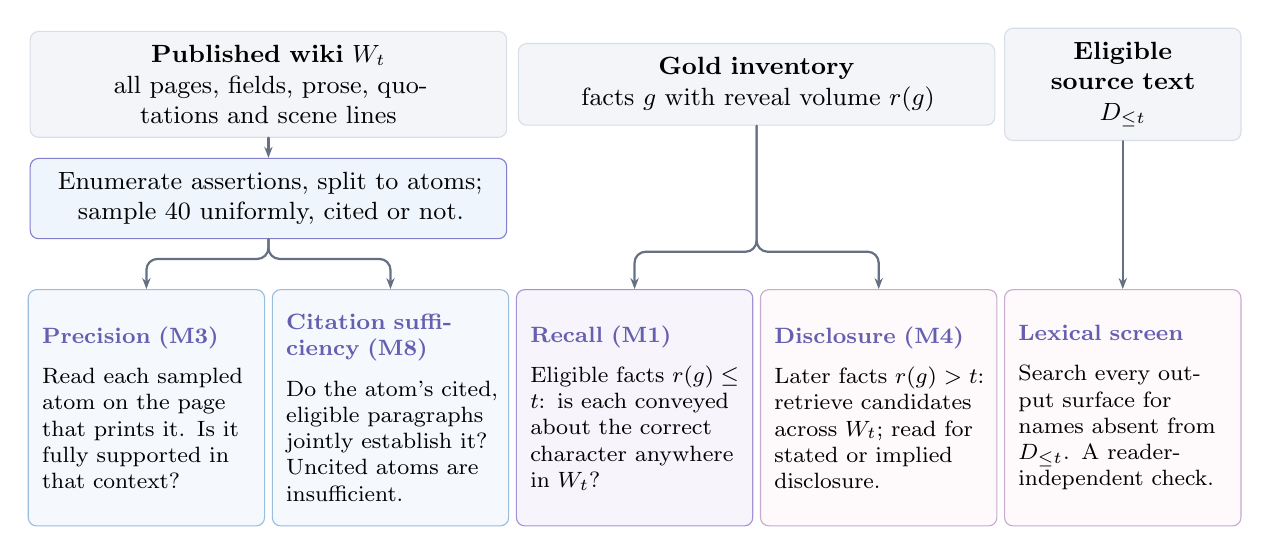
\begin{tikzpicture}[font=\small, x=1cm, y=1cm,
  source/.style={draw=nwgrid, fill=nwgraybg, rounded corners=3pt,
    align=center, inner sep=5pt, font=\small, minimum height=0.68cm},
  operation/.style={draw=nwblue!75!nwaccent, fill=nwbluebg, rounded corners=3pt,
    align=center, inner sep=5pt, font=\small},
  metric/.style={draw=#1!75!nwaccent, fill=white, rounded corners=3pt,
    align=left, text width=2.65cm, inner sep=5pt, anchor=north,
    font=\footnotesize, minimum height=3.0cm},
  arr/.style={-{Stealth[length=4pt]}, line width=0.8pt, draw=nwgray,
    rounded corners=4pt, line cap=round, line join=round},
]
\node[source, text width=5.7cm] (wiki) at (1.55,0)
  {\textbf{Published wiki $W_t$}\\all pages, fields, prose, quotations and scene lines};
\node[source, text width=5.7cm] (gold) at (7.75,0)
  {\textbf{Gold inventory}\\facts $g$ with reveal volume $r(g)$};
\node[source, text width=2.65cm] (text) at (12.4,0)
  {\textbf{Eligible source text}\\$D_{\le t}$};
\node[operation, text width=5.7cm] (sample) at (1.55,-1.45)
  {Enumerate assertions, split to atoms; sample 40 uniformly, cited or not.};
\node[metric=nwcyan, fill=nwbluebg!65] (precision) at (0,-2.6) {%
  {\color{nwaccent}\textbf{Precision (M3)}}\\[5pt]
  Read each sampled atom on the page that prints it. Is it fully supported in that context?};
\node[metric=nwcyan, fill=nwbluebg!65] (citation) at (3.1,-2.6) {%
  {\color{nwaccent}\textbf{Citation sufficiency (M8)}}\\[5pt]
  Do the atom's cited, eligible paragraphs jointly establish it? Uncited atoms are insufficient.};
\node[metric=nwviolet, fill=nwgreenbg!65] (recall) at (6.2,-2.6) {%
  {\color{nwaccent}\textbf{Recall (M1)}}\\[5pt]
  Eligible facts $r(g)\le t$: is each conveyed about the correct character anywhere in $W_t$?};
\node[metric=nwmagenta, fill=nwredbg!40] (disclosure) at (9.3,-2.6) {%
  {\color{nwaccent}\textbf{Disclosure (M4)}}\\[5pt]
  Later facts $r(g)>t$: retrieve candidates across $W_t$; read for stated or implied disclosure.};
\node[metric=nwmagenta, fill=nwredbg!40] (lexical) at (12.4,-2.6) {%
  {\color{nwaccent}\textbf{Lexical screen}}\\[5pt]
  Search every output surface for names absent from $D_{\le t}$. A reader-independent check.};
\draw[arr] (wiki.south) -- (sample.north);
\draw[arr] (sample.south) -- ++(0,-0.25) -| (precision.north);
\draw[arr] (sample.south) -- ++(0,-0.25) -| (citation.north);
\draw[arr] (gold.south) -- ++(0,-1.6) -| (recall.north);
\draw[arr] (gold.south) -- ++(0,-1.6) -| (disclosure.north);
\draw[arr] (text.south) -- (lexical.north);
\end{tikzpicture}

\caption{The evaluation protocol, applied identically to every system's wiki at every cutoff.
Cyan: support for the wiki's assertions. Lavender: coverage of information available to the
reader. Pink: checks for later information reaching the reader.}
\label{fig:protocol}
\end{figure*}

\paragraph{Annotators and workflow.} Labels were produced by LLM coding agents working
interactively in the project repository under the written rules of this appendix, not by
a fixed prompt: for each item the agent read the fact or assertion with the eligible source
paragraphs and recorded a label in a released label file. First-pass labels came from two
agents, OpenAI Codex and Claude Opus~5.5; Claude Opus~5.5 finalized every reported label.
The model version behind the Codex agent was not recorded.
The prefix-index builds of Table~\ref{tab:prefixv2} received a single pass.

\paragraph{How each metric is computed.} Let $A_t$ be the atomic assertions of $\Wt$, $S_t
\subset A_t$ the sampled atoms (40 drawn uniformly, with enumeration frame errors removed),
$c(a)$ the set of paragraphs cited for atom
$a$, $c_t(a)=c(a)\cap\Dt$ its eligible part, and $\mathbf{1}[\cdot]$ the indicator. For an assessed later fact $g\in\Ft$, $d_t(g)$ is
the verdict of reading every candidate sentence of $\Wt$ for it.
\begin{align*}
\text{M4}_t &= |P_t|\,/\,|\Ft| \qquad (t\le 4),\\
P_t &= \{g\in\Ft : d_t(g)\in\{\text{stated},\text{implied}\}\},\\
\text{M8}_t &= \frac{1}{|S_t|}\sum_{a\in S_t}\mathbf{1}\big[\sigma_t(a)\big],\\
\sigma_t(a) &\equiv c_t(a)\neq\varnothing \wedge c_t(a)\models a,\\
\text{CITE}_t &= \frac{|\{a\in A_t : c(a)\neq\varnothing\}|}{|A_t|},\\
\text{M5} &= \frac{|L|}{\sum_{t\le 4}|S_t|},\\
L &= \{(t,a) : 1\le t\le 4,\; a\in S_t,\\
  &\qquad \Dt\not\models a,\; D_{\le 5}\models a\},
\end{align*}
where $c_t(a)\models a$ means the eligible cited paragraphs, read alone and jointly, establish every element
of $a$ (\emph{sufficient} below); cited paragraphs after the cutoff are ignored, so an atom
citing only later paragraphs is insufficient. The disclosure count of Table~\ref{tab:main} is
$\sum_{t=1}^{4}|P_t|$; the inclusive count adds the facts whose verdict is \emph{uncertain}. A system's value is the unweighted mean over the cutoffs measured,
$\bar{M}=\frac{1}{|T|}\sum_{t\in T}M_t$. A paired difference between systems $A$ and $B$ is
$\Delta=\frac{1}{|T|}\sum_{t\in T}\big(M_t^{A}-M_t^{B}\big)$, each system scored on its whole
artifact against the same gold facts; its standard deviation, median, lowest and highest value are those of
the per-cutoff differences. The recall gap relative to the closed-book diagnostic is
$\bar{\text{M1}}-\bar{\text{M1}}{}^{X1}$; it does not isolate the contribution of reading
from memory. The seeded search recall is the share of seeded
disclosure sentences returned as candidates. M5 assesses a uniform assertion sample,
whereas M4 uses fact-directed searches across the delivered artifact; their denominators
and detection coverage differ.

\paragraph{Unit.} An atomic assertion states one predicate about one subject, and an object
for relations. Its interpretation includes polarity, modality, and attribution to the
speaker or believer when the narrative does not establish it as true.

\paragraph{Support labels (M3).} \emph{Supported}: the text through the cutoff establishes the
assertion with the stated attribution and modality. \emph{Partial}: part of it is established,
or a transient state is presented as a lasting trait. \emph{Unsupported}: nothing through the
cutoff establishes it. \emph{Uncertain}: the annotator cannot decide from the eligible text.
The annotator may read surrounding eligible context but never text after the cutoff. Only
\emph{supported} counts. Each atom is judged in the context of the page on which it appears;
its factuality in isolation is also recorded (\emph{true as a statement}). An error
introduced by the enumeration tool, such as assigning a quotation to the wrong speaker, is a
frame error and is excluded from the denominator (\res{M3-anne-frame}).

\paragraph{The pair rule.} Relationship pages display lines from scene summaries as shared
scenes. A factually true line is supported \emph{on that page} only if both characters are
present and participate in at least one episode of the scene summarized.
Being mentioned, quoted, written to, remembered, dead, or watching from a distance does not
count. This \emph{scene rule} is the standing one. Under the stricter \emph{line rule},
reported as a sensitivity value, the pair must take part in the episode that the sampled
line itself describes. An earlier rule that accepted a pair present anywhere in the chapter
was retired because it conflated shared scenes with shared chapters. The first-pass labels
of the first and the reported build had used different pair rules, so Claude Opus~5.5
re-read every sampled relationship line from the first build, reported build, and two
prefix builds against the chapter text. The annotator recorded verdicts under both the scene rule and the line rule. These contextual
verdicts are combined with each build's factuality labels to compute the page-context
precision reported here.

\paragraph{Reveal volume.} The earliest $t$ whose prefix $\Dt$ establishes the fact without
later text; foreshadowing that a first-time reader could not resolve is not sufficient. Each
later fact's reveal volume was checked against the earliest statement in the text by a keyword
scan of every earlier volume followed by a read; the check moved \res{OBS-gold-late} drafted
facts to an earlier volume.

\paragraph{Conveyed (M1).} A gold fact is conveyed at cutoff $t$ when any page of that
cutoff's wiki (a character, relationship, codex or timeline page) states its core proposition
of the right character (the same subject, the same event, relation or attribute, and the same
object) in any wording. A conjunction of two propositions needs both
(\emph{a newspaper man and a grandson of the schoolmaster}). An incidental qualifier may be
missing (\emph{four years ago}, \emph{at Christmas}, a color or a material); a wrong or
missing core element may not: who did it, to whom, or the number when the number is the fact
(\emph{Una is ten}). The same proposition asserted of a different character does not count (where the statement
stands does not matter, whom it is about does), and an engagement does not convey a marriage.
We formalized this rule across all systems after an audit of the first-pass recall labels
found it inconsistently applied. Labels had been carried forward across
cutoffs when similar wording persisted; a fact marked absent early was therefore not
reassessed when a later wiki paraphrased it. The audit rechecked every gold fact in every
system using one search pattern per fact and changed
\res{M1-anne-audit-changes} labels; the reported build of \sys and the graph baseline on it
were labeled afterward with the same patterns.

\paragraph{Disclosed (M4).} \emph{Stated}: a page asserts the later fact. \emph{Implied}: a
page asserts something from which a reader would infer it. \emph{Uncertain}: a page asserts
something adjacent that is available at the cutoff and that a reader could, but need not, read
toward the later fact. \emph{Absent}: no candidate sentence was found, or every candidate read
was about something else. Stated and implied count as disclosure. Candidates are found by
three lexical routes: vocabulary that first occurs after $t$, overlap with the content words
of the fact, and marriage, death and birth words near the character's name.

\paragraph{Citation sufficiency (M8).} For a sampled atom that the page cites, the annotator
opens every paragraph in the citation list of that line or section (only paragraphs at or
before the cutoff count) and asks whether they establish the atom without any other text.
\emph{Sufficient}: every element of the atom is in the cited paragraphs, jointly if need be; a
relation is sufficient when the paragraph states it of a person the reader can identify, even
if the page's canonical surname is given elsewhere. \emph{Partial}: the core is there and a
stated element is not (an added qualifier, a trait inferred from behavior).
\emph{Insufficient}: the supporting paragraph is not in the list, the list points to another
volume or person, or the atom is itself unsupported. An assertion with no paragraph citation is
insufficient; a link to a whole chapter is not a paragraph citation. Only \emph{sufficient}
counts. One correction was made after labeling. The tool that enumerates assertions did not
attach to a timeline line of the reported build the \emph{Sources} line printed under it, so
the 22 sampled timeline atoms had been labeled as uncited. Their citations were read from
the delivered pages and judged by the rule above: 11 are sufficient. Counting them as uncited
would give \sys a citation sufficiency of 0.457 instead of \respt{M8-anne-avg-B5}, and a share
of assertions with a paragraph citation of 0.840 instead of \res{CITE-anne-B5}.

\paragraph{The precision audit.} Citation assessment for M8 revealed comparison-system
atoms previously labeled unsupported or uncertain that were established by the text,
sometimes by the page's own citations. The first pass searched for a character's name near
the fact, missing pronoun references, and examined only the first six cited passages.
All \res{M3-anne-audit-read} comparison-system atoms not labeled supported were re-read
against the best-matching paragraphs of the complete eligible text, and
\res{M3-anne-audit-changes} were corrected to supported. The atom-level negatives of \sys's
first build were re-read the same way and none changed. Labels already marked supported were not re-audited for
any system.

\ifnwhuman
\paragraph{Two-reviewer agreement.}
Two human reviewers each labeled the complete review packet (\res{HREV-total}
original-text items: every gold fact and the samples of recall, precision and citation
labels listed below), giving two separate sets of final labels. Table~\ref{tab:human-agreement} recomputes their agreement on the original-text
validation tasks. Cohen's $\kappa$ is reported separately for gold evidence, recall,
precision and citation sufficiency, since these tasks have different questions and label
spaces. Across the \res{HREV-total} reviewed items, all assessed decisions agree on
\res{HREV-all-agree}; at least one decision differs on \res{HREV-any-disagreement}.
These values describe concordance between the reviewers' final judgments, rather than
agreement with the AI annotations or correctness of the annotations. Each reviewer labeled
every item from scratch, without seeing the AI answers, so these judgments are not anchored
on them.

% Source: supplied reviewer CSVs; recomputed_agreement_20261010.json.
\begin{table}[t]
\centering\small
\setlength{\tabcolsep}{4pt}
\renewcommand{\arraystretch}{1.12}
\begin{tabular}{@{}lrrr@{}}
\toprule
\nwhead{Task} & \nwhead{Items} & \nwhead{Agreement} & \nwhead{$\kappa$} \\
\midrule
Gold evidence & \res{HREV-G-n} & \res{HREV-G-agreement} & \res{HREV-G-kappa} \\
Recall (M1) & \res{HREV-R-n} & \res{HREV-R-agreement} & \res{HREV-R-kappa} \\
Precision (M3) & \res{HREV-P-n} & \res{HREV-P-agreement} & \res{HREV-P-kappa} \\
Citation (M8) & \res{HREV-C-n} & \res{HREV-C-agreement} & \res{HREV-C-kappa} \\
\midrule
Pair placement & \res{HREV-PAIR-n} & \res{HREV-PAIR-agreement} & \res{HREV-PAIR-kappa} \\
\bottomrule
\end{tabular}
\caption{Agreement between the two human reviewers' final labels.
Cohen's $\kappa$ is reported per task; no mixed-task coefficient is pooled.
Pair placement is a precision subset, not additional items.}
\label{tab:human-agreement}
\end{table}


Table~\ref{tab:human-ai-agreement} compares each reviewer's label set with the accepted
AI-assisted review snapshot finalized by Claude. Its mapping to the accepted source sheet
is verified; it is not independently verified as unchanged blind first-pass AI labels.
Each comparison uses all \res{HRAI-total} reviewed items. Pair placement is evaluated separately on
\res{HRAI-PAIR-n} relationship-page items within the precision sample.
All applicable decisions agree on \res{HRAI-r1-all-agree} items for reviewer~1, with at least
one disagreement on \res{HRAI-r1-any-disagreement}; for reviewer~2, the corresponding counts
are \res{HRAI-r2-all-agree} and \res{HRAI-r2-any-disagreement}.
These comparisons measure reviewer--AI concordance, not annotation accuracy.

\paragraph{Reviewer provenance.}
Both final label sets were produced entirely by human reviewers; no model generated or
proposed these decisions. Both CSVs cover the complete review
packet, and their labels match the accompanying response records. A released aligned audit
maps each decision to its original item and marks remaining disagreements as unadjudicated.

% Source: supplied reviewer CSVs and accepted_answers.csv; recomputed_agreement_20261010.json.
\begin{table*}[t]
\centering\small
\setlength{\tabcolsep}{8pt}
\renewcommand{\arraystretch}{1.12}
\begin{tabular}{@{}lrrrrr@{}}
\toprule
\nwhead{Task} & \nwhead{Items} & \multicolumn{2}{c}{\nwhead{Reviewer 1 vs.\ AI}} & \multicolumn{2}{c}{\nwhead{Reviewer 2 vs.\ AI}} \\
\cmidrule(lr){3-4}\cmidrule(lr){5-6}
& & \nwhead{Agreement} & \nwhead{$\kappa$} & \nwhead{Agreement} & \nwhead{$\kappa$} \\
\midrule
Gold evidence & \res{HRAI-G-n} & \res{HRAI-r1-G-agreement} & \res{HRAI-r1-G-kappa} & \res{HRAI-r2-G-agreement} & \res{HRAI-r2-G-kappa} \\
Recall (M1) & \res{HRAI-R-n} & \res{HRAI-r1-R-agreement} & \res{HRAI-r1-R-kappa} & \res{HRAI-r2-R-agreement} & \res{HRAI-r2-R-kappa} \\
Precision (M3) & \res{HRAI-P-n} & \res{HRAI-r1-P-agreement} & \res{HRAI-r1-P-kappa} & \res{HRAI-r2-P-agreement} & \res{HRAI-r2-P-kappa} \\
Citation sufficiency (M8) & \res{HRAI-C-n} & \res{HRAI-r1-C-agreement} & \res{HRAI-r1-C-kappa} & \res{HRAI-r2-C-agreement} & \res{HRAI-r2-C-kappa} \\
\midrule
Pair placement & \res{HRAI-PAIR-n} & \res{HRAI-r1-PAIR-agreement} & \res{HRAI-r1-PAIR-kappa} & \res{HRAI-r2-PAIR-agreement} & \res{HRAI-r2-PAIR-kappa} \\
\bottomrule
\end{tabular}
\caption{Agreement recomputed for each human reviewer's label set against the accepted
AI-assisted reference snapshot. Each comparison uses all \res{HRAI-total} reviewed items.
Pair placement is reported separately for a subset of the precision sample;
its items are not added to the total. No mixed-task coefficient is pooled.}
\label{tab:human-ai-agreement}
\end{table*}


\paragraph{Joint agreement across the three label sets.}
Table~\ref{tab:human-alpha} recomputes nominal Krippendorff's $\alpha$ for the same accepted
AI-assisted reference and the two reviewers' final-label sets. All \res{HRAL-total}
items have complete labels from all three. For each task, $\alpha=1-D_o/D_e$ uses nominal
distance (zero for identical labels, one otherwise), observed within-item coincidences,
and expected disagreement from pooled category counts with the $n(n-1)$ finite-sample
correction, where $n$ is the number of pairable label values
\citep[pp.~1--5]{krippendorff2011alpha}. It is calculated jointly, rather than by averaging
pairwise kappas. Pair placement is again assessed separately within the precision sample.
The coefficient measures concordance among the AI labels and two human label sets;
it is not an all-human reliability estimate or an accuracy measure. The recomputed
coefficients match the summary distributed with the label files. This calculation
reproduces decisions; it does not adjudicate disagreements or change system scores.

% Source: supplied reviewer CSVs and accepted_answers.csv; recomputed_agreement_20261010.json.
\begin{table*}[t]
\centering\small
\setlength{\tabcolsep}{8pt}
\renewcommand{\arraystretch}{1.12}
\begin{tabular}{@{}lrrrr@{}}
\toprule
\nwhead{Task} & \nwhead{Items} & \nwhead{$\alpha$} & \nwhead{Mean pairwise agreement} & \nwhead{Unanimous items} \\
\midrule
Gold evidence & \res{HRAL-G-n} & \res{HRAL-G-alpha} & \res{HRAL-G-agreement} & \res{HRAL-G-unanimous} \\
Recall (M1) & \res{HRAL-R-n} & \res{HRAL-R-alpha} & \res{HRAL-R-agreement} & \res{HRAL-R-unanimous} \\
Precision (M3) & \res{HRAL-P-n} & \res{HRAL-P-alpha} & \res{HRAL-P-agreement} & \res{HRAL-P-unanimous} \\
Citation sufficiency (M8) & \res{HRAL-C-n} & \res{HRAL-C-alpha} & \res{HRAL-C-agreement} & \res{HRAL-C-unanimous} \\
\midrule
Pair placement & \res{HRAL-PAIR-n} & \res{HRAL-PAIR-alpha} & \res{HRAL-PAIR-agreement} & \res{HRAL-PAIR-unanimous} \\
\bottomrule
\end{tabular}
\caption{Nominal Krippendorff's $\alpha$ recomputed jointly over the accepted
AI-assisted reference and the two human reviewers' final-label sets. All \res{HRAL-total}
items have complete labels from all three. Mean pairwise agreement averages the three
label-set pairs; unanimous items have identical labels in all three sets.
Pair placement is a subset of precision, not additional items. No mixed-task $\alpha$ is pooled.}
\label{tab:human-alpha}
\end{table*}

\fi

\paragraph{Earlier human review.} Claude Opus~5.5 finalized all reported AI labels.
\ifnwhuman Before the two-reviewer check, one human reviewer examined and accepted an
AI-checked sheet with answers and reasons visible; this pass yields no agreement estimate.
It assessed the labels \else The planned human check is not included
in this version; every reported value is an LLM label. It assesses the labels \fi against
the source text and the rules above. Sets of at most 500 items are checked in full; larger
sets use a uniform random 10\% sample. Each set is checked separately:
\begin{itemize}[nosep,leftmargin=*]
\item gold facts, \res{ANN-n-gold} items (at most 500): every fact and its evidence paragraph;
\item recall labels, \res{ANN-n-recall} items (over 500): a sample of \res{ANN-n-recall-sample};
\item precision atoms, \res{ANN-n-precision} items (over 500): a sample of \res{ANN-n-precision-sample};
\item citation-sufficiency labels, \res{ANN-n-m8} items (over 500): a sample of \res{ANN-n-m8-sample};
\item disclosure verdicts, \res{ANN-n-m4} items, and the \res{M4-cand-anne-all} candidate
  sentences behind them: not checked by a human; these are LLM labels only.
\end{itemize}
In all, \res{ANN-n-total} labels \ifnwhuman were reviewed\else are checked by a human\fi.
The sampling frame was fixed before the last labels were added: its precision atoms are
those of every original-text cell then labeled, including prefix-build cells, and its
citation labels are those of B1, B2 and \sys; the citation labels of B3, B4 and X2 were
added later and are outside it.
\ifnwdecon All of them are labels of the original text: the labels of the treated text
(Appendix~\ref{app:contamination}) were finalized afterward by Claude and
are not part of the check.
\fi
\ifnwhuman The accepted answers agree with the paper's original labels on
\res{HUMR-recall-same} recall items, \res{HUMR-precision-same} precision atoms and
\res{HUMR-m8-same} citation labels. Of the gold facts, \res{HUMR-gold} are established by
their evidence paragraph in full, in part and not at all; \res{HUMR-gold-announce} of those
established in part are dated by a paragraph that announces the event, which is completed
within the same volume, so no reveal volume moves. For the three not established, the fact
holds in the volume it is dated to, but the paragraph recorded as its evidence does not carry
it alone (a greeting for a household arrangement, a plan for a residence, an introduction
that does not yet tie a surname to the man). In recall and precision the accepted
answers are stricter; citation-sufficiency differences occur in both directions.

The recall differences had one cause: in some cells a page sentence weaker than the gold fact
had been credited (``fascinated by insects'' for a boy who collects toads, bugs and frogs; a
fight for a hatred). The written rule already asked for the same event, relation or
attribute. We therefore re-read six gold facts in every cell of every system, on both texts,
with one test per fact, and changed \res{HUMR-strict-changes} recall labels. The re-read
moved no system's mean recall by more than 0.021 and is in every value reported here; after
it the accepted answers match \res{HUMR-recall-same-after} recall items. It covers the six
facts the check surfaced, not all \res{ANN-n-gold}. Precision and citation labels were not
changed on the sampled items alone, since that would correct a tenth of the labels under a
reading the other nine tenths did not get.\fi

\paragraph{Zero counts.} A zero disclosure count is printed as $0/n$. Under an idealized
model of $k$ independent, representative character-level Bernoulli trials with zero events,
where $k$ is the number of characters with an assessed later fact at $t$ (40 at $t=1$, 12
at $t=4$), the exact one-sided 95\% upper bound is $1-0.05^{1/k}$:
\res{M4-anne-bound-t1} at $t=1$ and \res{M4-anne-bound-t4} at $t=4$.
Grouping by character avoids treating correlated assertions as independent. However,
characters also interact, the cast is purposively selected, and candidate retrieval is
incomplete. These values illustrate the effect of the sampling unit; they are not
calibrated population bounds on this system's spoiler risk.

% Appendix: corpus documentation.
\section{Corpus and Evaluation Dataset}
\label{app:corpus}

% T1: the evaluated corpus by volume, with gold counts by cutoff.
\begin{table}[t]
\centering\small
\setlength{\tabcolsep}{2pt}
\begin{tabular}{@{}clrrrrr@{}}
\toprule
\nwhead{$t$} & \nwhead{Book} & \nwhead{Par.} & \nwhead{Words} & \nwhead{Ch.} & \nwhead{$|\Gt|$} & \nwhead{$|\Ft|$} \\
\midrule
1 & \emph{Anne of Green Gables} & \res{T1-anne-v1-par} & \res{T1-anne-v1-words} & \res{T1-anne-v1-ch} & \res{T1-anne-gold-t1} & \res{T1-anne-future-t1} \\
2 & \emph{Anne of Avonlea} & \res{T1-anne-v2-par} & \res{T1-anne-v2-words} & \res{T1-anne-v2-ch} & \res{T1-anne-gold-t2} & \res{T1-anne-future-t2} \\
3 & \emph{Anne of the Island} & \res{T1-anne-v3-par} & \res{T1-anne-v3-words} & \res{T1-anne-v3-ch} & \res{T1-anne-gold-t3} & \res{T1-anne-future-t3} \\
4 & \emph{Anne's House of Dreams} & \res{T1-anne-v4-par} & \res{T1-anne-v4-words} & \res{T1-anne-v4-ch} & \res{T1-anne-gold-t4} & \res{T1-anne-future-t4} \\
5 & \emph{Rainbow Valley} & \res{T1-anne-v5-par} & \res{T1-anne-v5-words} & \res{T1-anne-v5-ch} & \res{T1-anne-gold-t5} & \res{T1-anne-future-t5} \\
\midrule
 & Total & \best{\res{T1-anne-paras}} & \best{\res{T1-anne-words}} & \best{\res{T1-anne-chapters}} & & \\
\bottomrule
\end{tabular}
\caption{The evaluated corpus. Paragraphs, words and chapters are per volume; $|\Gt|$ is the
number of gold facts eligible at cutoff $t$ and $|\Ft|$ the number of later facts assessed for
disclosure at $t$.}
\label{tab:corpus}
\end{table}


\paragraph{Editions.} The Anne series is read from Project Gutenberg eBooks 45 (\emph{Anne of
Green Gables}), 47 (\emph{Anne of Avonlea}), 51 (\emph{Anne of the Island}), 544 (\emph{Anne's
House of Dreams}) and 5343 (\emph{Rainbow Valley}), in that order (Table~\ref{tab:corpus}).
The corpus follows the publication order of the first five Anne books (1908--1919), excluding
two later-written books set between them. Throughout the paper, a volume is one book; word
counts use whitespace-delimited tokens in the parsed text.

\paragraph{Development history.} The pipeline was developed on other series,
which contribute no reported results. The Anne books were processed while the pipeline was
still being revised, so this corpus is not a held-out evaluation. Baseline settings were chosen on George
Eliot's \emph{Middlemarch} (Gutenberg eBook 145, Books I--V) and not on the Anne series
(Appendix~\ref{app:baselines}).

\paragraph{Cast.} The evaluated cast contains the \res{T1-anne-cast} characters with at least one
gold fact. A comparison system generates a character page at cutoff $t$ if a gold fact about
that character is evidenced by $t$ or their full name occurs in $\Dt$. Characters without a
page remain in the evaluation denominators. This rule replaces an earlier rule that matched
any single word of a name and generated baseline pages for characters not yet introduced
(Appendix~\ref{app:casebook}).

\paragraph{Dataset size and units.}
The source corpus contains \res{T1-anne-words} whitespace-delimited words in
\res{T1-anne-paras} paragraphs and \res{T1-anne-chapters} chapters. The evaluated inventory
contains \res{T1-anne-gold-t5} selected facts about \res{T1-anne-cast} characters.
Table~\ref{tab:dataset-size} distinguishes these unique records from repeated judgments.
Each original or treated condition contains the same seven systems at five cutoffs;
renaming and paraphrasing reuse the inventory and reveal dates rather than adding an
independent corpus. Recall labels judge eligible fact--cutoff pairs; disclosure labels judge
later fact--cutoff pairs. Assertions are a separate system-generated population sampled
for precision and citation sufficiency. Repeated cutoffs share facts and characters.

\begin{table}[t]
\centering\small
\setlength{\tabcolsep}{4pt}
\begin{tabular}{@{}lrr@{}}
\toprule
\nwhead{Primary-matrix unit} & \nwhead{Original} & \nwhead{Treated} \\
\midrule
System--cutoff artifacts & \res{DATA-orig-artifact-cells} & \res{DATA-treated-artifact-cells} \\
Selected gold records & \res{T1-anne-gold-t5} & \res{T1-anne-gold-t5} \\
Cast characters & \res{T1-anne-cast} & \res{T1-anne-cast} \\
Recall judgments & \res{DATA-orig-recall-assessments} & \res{DATA-treated-recall-assessments} \\
Disclosure judgments & \res{DATA-orig-disclosure-assessments} & \res{DATA-treated-disclosure-assessments} \\
Sampled assertion records & \res{DATA-orig-precision-sample-rows} & \res{DATA-treated-precision-sample-rows} \\
Excluded frame errors & \res{DATA-orig-precision-frame-errors} & \res{DATA-treated-precision-frame-errors} \\
Evaluated precision atoms & \res{DATA-orig-precision-evaluated-atoms} & \res{DATA-treated-precision-evaluated-atoms} \\
\bottomrule
\end{tabular}
\caption{Size of the primary evaluation matrix, excluding earlier and prefix-build diagnostics.
Counts describe records and judgments, not independent trials. Both conditions reuse the same
gold inventory. Citation sufficiency uses the sampled assertion records; X1 supplies no citations.}
\label{tab:dataset-size}
\end{table}


\paragraph{What a record contains.}
The gold YAML groups facts by character. Each fact records a claim and a paragraph identifier;
the identifier encodes its evidence volume, chapter and paragraph. Optional keyword lists
assist disclosure search, while reader and note fields record provenance. The stored YAML
retains historical later-volume entries, but this evaluation selects evidence volumes
one to five only. Below is a minimal excerpt from an existing record, with provenance
metadata omitted:

\begin{lstlisting}[basicstyle=\ttfamily\scriptsize]
series: anne
characters:
  Matthew Cuthbert:
    facts:
      - claim: "Matthew is the shyest man alive."
        evidence: v01:c01:p0004
\end{lstlisting}

\paragraph{Easier example: a direct statement.}
The cited paragraph describes Matthew as ``the shyest man alive'' and says that he
``hated to have to go among strangers''. The human-accepted gold check
(Appendix~\ref{app:annotation}) labels this record fully supported. The character and description occur together, so matching
the proposition requires neither a cross-paragraph identity link nor a conjunction.
Its evidence volume is one: it is eligible at every evaluated cutoff. This is the
narrator's characterization of Matthew, rather than a claim about his current life status.

\paragraph{Harder example: conjunction and local coreference.}
Owen Ford's record reads: ``Owen Ford is a newspaper man and a grandson of the schoolmaster
who built the house'', with evidence \pid{v04:c22:p0019}. Miss Cornelia's report includes
``His name is Owen Ford'', ``a newspaper man'' and ``a grandson of the schoolmaster who
built this house''. The human-accepted gold check labels the record fully supported.
Interpreting the pronouns requires linking them to Owen; recall requires both the
occupation and the family/house relation. A generated statement that supplies only his
occupation does not convey the full record. At cutoff three the fact is a disclosure probe;
at cutoff four it becomes eligible. The example illustrates the existing conjunction
rule, not a measured difficulty grade or a newly assigned annotation.

\paragraph{An evidence boundary case.}
The gold claim ``Anne marries Gilbert Blythe'' points to \pid{v04:c04:p0000}, which begins
``Anne wakened on the morning of her wedding day''. That paragraph alone neither names
Gilbert nor establishes the completed marriage. The human-accepted gold check
therefore marks it partial, even though the fact is assigned to the correct volume.
This example distinguishes volume-level support from paragraph-level evidence sufficiency;
the recorded evidence defect remains part of the inventory, as reported in
Appendix~\ref{app:annotation}. These illustrative cases do not constitute new labels,
a measured easy/hard split, or a repair of the gold evidence.

\paragraph{Review population and release scope.}
The two-reviewer check covers \res{ANN-n-total} original-text items:
\res{ANN-n-gold} gold-evidence, \res{ANN-n-recall-sample} recall,
\res{ANN-n-precision-sample} precision and \res{ANN-n-m8-sample} citation checks, sampled
from the labels that existed when the sample was drawn (Appendix~\ref{app:annotation}).
Original and treated gold, per-system judgments, sampled assertions, candidate witnesses,
the two reviewers' final label files and recomputed agreement form the evaluation materials. The reviewer files, original response records and input
hashes are released; the human review is described in Appendix~\ref{app:annotation}.

% Appendix: implementation. Values are those of the configuration used for the reported build.
\section{Implementation Details}
\label{app:implementation}

\begin{algorithm*}[t]
\caption{Assembling the page of entity $e$ at cutoff $t$.}
\label{alg:assemble}
\small
\begin{algorithmic}[1]
\Require graph of verifier-accepted intervals; entity $e$; cutoff $t$
\State $I \gets$ copies of $\{\, i \in \textsc{Intervals}(e) : i.\mathit{start} \le t \,\}$ \Comment{a local view; the graph is not modified}
\If{$I = \varnothing$} \Return no page \Comment{an entity with no interval by $t$ has no page and is no link target}
\EndIf
\For{$i \in I$}
  \State $i.\mathit{quotes} \gets \{\, q \in i.\mathit{quotes} : \mathrm{vol}(q) \le t \,\}$ \Comment{each quote filtered by its own volume}
  \If{$i.\mathit{end} > t$} \State $i.\mathit{end} \gets \bot$ \Comment{do not reveal that, or when, it ends}
  \EndIf
\EndFor
\State $I \gets \{\, i \in I : \textsc{Verified}(i) \,\}$ \Comment{facts the verifier rejected are withheld}
\State $\mathit{fields} \gets \textsc{Render}(I)$ \Comment{deterministic: names, attributes, relations, history}
\State $\mathit{prose} \gets \textsc{Generate}(I)$ \Comment{model sees only $I$; no evidence $\Rightarrow$ no call, empty section}
\State $\mathit{page} \gets \textsc{Link}(\mathit{fields}, \mathit{prose}, \{\, s : \mathrm{vol}(s) \le t \,\})$ \Comment{surface forms and targets revealed by $t$}
\State \Return $\mathit{page}$ with cutoff-$t$ title and navigation
\end{algorithmic}
\end{algorithm*}

\paragraph{Claim schema.} A claim is a record with a subject (an entity identifier, never a
raw surface form), a predicate, a kind (attribute, relation or trait), an object entity or a
scalar value, an optional short qualifier, a polarity (asserted, denied or presumed), the
volume and chapter of its first evidence, and one or more evidence items, each a paragraph
identifier with a verbatim quote of at most 240 characters. \emph{Presumed} is meant to keep a belief
apart from a fact: a character thought dead in one volume is recorded as presumed dead there,
not as dead. The renderer marks a presumed value in attribute and relation lines, but the
infobox's family field and the list of related characters print it unmarked
(Section~\ref{sec:results-main}). Polarity and qualifier are part of a claim's identity, so two observations that
disagree on either never merge. A claim whose subject or object cannot be resolved to a known
entity is dropped.

\paragraph{Ontology.} Entities are typed as character, group, place, event or object; only
characters get their own pages, and the other types share codex pages. There are nine
attributes (age, gender, status, rank, title, nickname, origin, occupation, appearance), five
trait keys (personality, motivation, skill, fear, background) and twenty relation predicates
covering kinship (parent, child, sibling, relative, spouse), affect (romantic, friend, rival,
enemy), roles (mentor, student, commands, serves under, comrade, affiliated with) and events
(origin, participated in, pilots, killed, saved). The ontology is shared by all series and was
not adapted to the evaluated work.

\paragraph{Extraction settings.} The chapter pass reads spans of about 4{,}000 tokens with 500
tokens of overlap and records, for each scene, a summary, the characters who take part and up
to four paragraphs that support the summary. The mention pass reads a window of four
paragraphs before and after a mention, never across a hard scene break, with at most 40
windows per entity per volume, one window per call and at most 6{,}000 tokens per window (a
denser cluster of mentions is split into consecutive windows). The long-context pass reads all of a character's paragraphs in a volume
(up to 150{,}000 tokens) for gender, age and origin, and separately for background. A claim
needs a self-reported confidence of at least 0.5 to be kept and 0.7 to fill a structured
field. An evidence-adequacy gate rejects quotes shorter than six words, quotes in which the
subject is not named within one paragraph, and quotes carrying irrealis markers (``would
have'', ``might have'').

\paragraph{Intervals.} Single-valued attributes supersede: a value's interval closes when the
next distinct value first appears. Relations in a declared conflict group supersede the same
way; every other relation and multi-valued attribute is an open interval that opens at its
earliest evidence, with its qualifier taken from evidence no later than that volume. Free-text
values whose BGE-M3 embeddings have cosine similarity of at least 0.86 are clustered before
intervals are built.

\paragraph{Generation.} Every model call uses \res{GEN-model}. The intended character-page
template specifies appearance 2--4, personality 2--6, and history 3--12 sentences; shared-page
summaries request one sentence. The archived \sys appearance prompt instead requests
3--4 sentences (Appendix~\ref{app:prompts}). These are prompt requirements, not a measurement
of output-length enforcement. Generation prompts request keys identifying the input lines
supporting the text, which map back to source paragraphs. The parser also normalizes returned
paragraph IDs during citation resolution, as in the codex example below. A shared-page
summary is retained only if a second call judges every statement to be established by its
input passages. A rejected summary is regenerated once and omitted if it fails again.
Responses are cached by provider, model, prompt, and parameters, so rebuilding an unchanged
configuration requires no new calls. All prompts are released verbatim with the code.
Prompts for \sys and text-reading comparison systems do not state the work's title or
author, but mined names can carry it: the series title is an entity in \sys's extraction
prompts, and the typing model's exhibited output names the novel (Appendix~\ref{app:prompts-full}).
The closed-book diagnostic receives the title by design.
A character with no STATUS claim is printed as \emph{alive (assumed)}: a configured
default with no evidence behind it, marked as assumed on the page, since the absence of a
death claim does not establish that a character is alive.

\paragraph{Prompt and response defects.} The extraction prompt of the reported runs
exposes internal revision labels, module paths, and implementation notes in the STATUS and
APPEARANCE descriptions. The prompt builder passes the same canonicalization note to the
verifier as the \emph{definition} of APPEARANCE, which the verifier is told to judge
against; a rule for deduplicating values does not define a physical characteristic. The
exhibited call accepts its appearance claim; the effect on other decisions is not measured.
The codex response returns a paragraph ID where the prompt requests an input-line key; the
parser maps it to its paragraph during citation resolution, without checking that the
paragraph supports the sentence. All reported results use this configuration; a repaired
prompt builder would require new runs, which this paper does not report.

\paragraph{Changes between builds.} The reported build differs from the first
build (Section~\ref{sec:results-quality}, Table~\ref{tab:builds}) by one batch of changes,
made after the first build had been labeled and applied to every series alike.
\emph{Entity resolution:} a bare name and a fuller name first seen in a later volume go to
the model instead of merging for free; a first name shared by several people is assigned per
volume; fuzzy matching may not exchange a whole word; the cap on model-judged name pairs
rose from 1{,}000 to 5{,}000; hyphenated names and titles of the form ``X of the Y'' are
mined whole. \emph{Ingestion:} publisher's back matter is dropped. \emph{Scenes:} the
participants of a scene are those who take part, not those mentioned, and each summary names
up to four supporting paragraphs. \emph{Citations:} generated text names the input lines it
rests on, and scene lines print their paragraphs on timeline, pair and codex pages; the first
build cited a chapter for a scene line and nothing for most prose. \emph{Gates:} a prose
answer that says it found nothing is discarded, and summaries on shared pages pass the check
described above. \emph{Windows:} the 6{,}000-token ceiling on a mention window, which the
first build did not enforce on a dense cluster. One side effect: the first
build held two entities for several main characters, and each entity received its own
windows, so the same text was read twice; with the entities merged it is read once, and the
claims stored for two such characters fell from 162 and 66 to 118 and 46 on as many windows.
We did not isolate this change's contribution to the reported build's lower recall.

% Appendix: baseline adaptations and settings.
\section{Comparison Systems}
\label{app:baselines}

All comparison systems (B1--B4, X1, X2) use the same cast list, character-page template,
generator, and intended character-page budget:
the shared sections and sentence limits (appearance 2--4, personality 2--6, history 3--12), at most five
quotes, and a shared citation format (Table~\ref{tab:baselines}). For systems supplied with
passages, citations to paragraphs outside their input are removed, and characters absent
from the eligible text receive no page but remain in the evaluation denominators. Settings were chosen on the development novel
(\emph{Middlemarch}) and fixed before the Anne runs. \sys itself is not given the cast: it
discovers entities and also publishes pages for other characters, relationships,
codex entries, and a timeline. The shared template therefore controls the evaluated cast's
character pages, while the complete artifacts differ in scope (Table~\ref{tab:kinds}).
The exhibited comparison prompts request 2--4 appearance sentences; the archived \sys
appearance prompt requests 3--4 (Appendix~\ref{app:prompts}). The template budget therefore
does not imply identical prompt wording or verified enforcement of output length.


\begin{table}[t]
\centering\small
\begin{tabular}{@{}lp{6.5cm}@{}}
\toprule
 & \nwhead{Adaptation and settings} \\
\midrule
B1 & Every paragraph of volumes $1,\ldots,t$, labeled with its identifier, precedes the task so that pages at a cutoff share a cacheable prefix. Prompts exceeding the model's context limit would be marked unsupported rather than truncated; none exceeded it. \\
B2 & Prefix-only index of consecutive paragraphs within a chapter (150 words). Okapi BM25 ($k_1{=}1.5$, $b{=}0.75$) and BGE-M3 cosine rankings for the character name alone and with seven facet words (appearance, personality, family, relations, goals, past, speech), fused by reciprocal rank ($k{=}60$); chunks added in fused order up to 20{,}000 tokens of retrieved text, then restored to reading order. Budgets count retrieved text only, estimated as characters divided by four, so a call's provider-counted input, which adds the prompt, can exceed them. Chunk size (150 or 300 words) and budget (6{,}000, 12{,}000 or 20{,}000 tokens) were chosen at $t{=}2$ of the development novel. \\
B3 & LightRAG 1.5.7, default chunking (1{,}200 tokens) and its default extraction prompt and limits (at most 100 rows and 40 entities per chunk), mode \texttt{mix}, context capped at the same 20{,}000 tokens, reranking off. The index at cutoff $t$ is the index at $t{-}1$ plus volume $t$, so no index sees a later volume. LightRAG supplies retrieval only: its retrieved entities, relations and chunks are passed to the shared generator, and its own extraction calls use the same model. \\
B4 & The \sys graph built from all five volumes. For each character, the facts visible at $t$ and their evidence paragraphs of volumes $\le t$, up to the same budget, are passed to the shared generator in place of \sys's structured rendering (graph \texttt{anne@v2}). \\
X1 & The shared prompt with the work's title, the character's name and no passages, with an instruction to write what is known of the character up to volume $t$; citations are empty by construction. \\
X2 & Every paragraph of volumes 1--5 regardless of $t$, with the instruction to write for a reader of volume $t$ and reveal nothing later. \\
\bottomrule
\end{tabular}
\caption{Adaptations of the comparison systems.}
\label{tab:baselines}
\end{table}

% Appendix: results at every cutoff.
\section{Results at Every Cutoff}
\label{app:full-results}

% T2: main comparison (two-column table*). Means over cutoffs; every cell is in Appendix E.
% The decontaminated block is tables/t2b-decon.tex, read only under \nwdecontrue.
\begin{table*}[t]
\centering\small
\setlength{\tabcolsep}{2.4pt}
\begin{tabular}{@{}llccccrr@{}}
\toprule
 &  & \multicolumn{1}{c}{\nwhead{Recall}} & \multicolumn{1}{c}{\nwhead{Precision}} & \multicolumn{1}{c}{\nwhead{Citation}} & \nwhead{Later facts} & \nwhead{Distinct} & \nwhead{Tokens} \\
\multicolumn{2}{@{}l}{\nwhead{System (cutoff enforced by)}} & \multicolumn{1}{c}{\nwhead{$\uparrow$}} & \multicolumn{1}{c}{\nwhead{$\uparrow$}} & \multicolumn{1}{c}{\nwhead{sufficiency $\uparrow$}} & \nwhead{disclosed $\downarrow$} & \nwhead{assertions} & \nwhead{in / out (M)} \\
\midrule
B1 & Long context (input) & \cellcolor{nwhighcyan}\best{\res{M1-anne-avg-B1}}\sdev{\res{STAT-M1-B1-sd}} & \res{M3-anne-avg-B1}\sdev{\res{STAT-M3-B1-sd}} & \res{M8-anne-avg-B1}\sdev{\res{STAT-M8-B1-sd}} & \res{M4-anne-total-B1} & \res{ND-anne-avg-B1} & \res{TOK-anne-B1} \\
B2 & Prefix retrieval (input) & \res{M1-anne-avg-B2}\sdev{\res{STAT-M1-B2-sd}} & \res{M3-anne-avg-B2}\sdev{\res{STAT-M3-B2-sd}} & \res{M8-anne-avg-B2}\sdev{\res{STAT-M8-B2-sd}} & \res{M4-anne-total-B2} & \res{ND-anne-avg-B2} & \cellcolor{nwhighviolet}\best{\res{TOK-anne-B2}} \\
B3 & LightRAG (input) & \res{M1-anne-avg-B3}\sdev{\res{STAT-M1-B3-sd}} & \res{M3-anne-avg-B3}\sdev{\res{STAT-M3-B3-sd}} & \res{M8-anne-avg-B3}\sdev{\res{STAT-M8-B3-sd}} & \res{M4-anne-total-B3} & \res{ND-anne-avg-B3} & \res{TOK-anne-B3} \\
B4 & Graph baseline & \res{M1-anne-avg-B4}\sdev{\res{STAT-M1-B4-sd}} & \cellcolor{nwhighcyan}\best{\res{M3-anne-avg-B4}}\sdev{\res{STAT-M3-B4-sd}} & \cellcolor{nwhighcyan}\best{\res{M8-anne-avg-B4}}\sdev{\res{STAT-M8-B4-sd}} & \res{M4-anne-total-B4} & \res{ND-anne-avg-B4} & +\res{TOK-anne-B4} \\
B5 & \sys (data) & \res{M1-anne-avg-B5}\sdev{\res{STAT-M1-B5-sd}} & \res{M3-anne-avg-B5}\sdev{\res{STAT-M3-B5-sd}} & \res{M8-anne-avg-B5}\sdev{\res{STAT-M8-B5-sd}} & \cellcolor{nwhighpink}\best{\res{M4-anne-total-B5}} & \cellcolor{nwhighviolet}\best{\res{ND-anne-avg-B5}} & \res{TOK-anne-B5} \\
\midrule
X1 & Closed book (none) & \res{M1-anne-avg-X1}\sdev{\res{STAT-M1-X1-sd}} & \res{M3-anne-avg-X1}\sdev{\res{STAT-M3-X1-sd}} & -- & \cellcolor{nwhighpink}\best{\res{M4-anne-total-X1}} & \res{ND-anne-avg-X1} & \res{TOK-anne-X1} \\
X2 & Full text (instruction) & \res{M1-anne-avg-X2}\sdev{\res{STAT-M1-X2-sd}} & \res{M3-anne-avg-X2}\sdev{\res{STAT-M3-X2-sd}} & \res{M8-anne-avg-X2}\sdev{\res{STAT-M8-X2-sd}} & \cellcolor{nwhighpink}\best{\res{M4-anne-total-X2}} & \res{ND-anne-avg-X2} & \res{TOK-anne-X2} \\
\bottomrule
\end{tabular}
\caption{Main comparison on Anne: rates are mean $\pm$ sample standard deviation across
$t=1..5$. Recall uses eligible gold facts; precision and citation sufficiency use 40 sampled
atoms per cutoff, judged in page context. Disclosure counts stated or implied later facts
across $t=1..4$. Distinct assertions are means per cutoff; tokens (millions, input / output)
cover the reported build. X1 and X2
are diagnostics; X1 cites nothing. Bold identifies rate and assertion-count maxima and
minimum measured cost among B1--B5, plus non-zero disclosures. Cyan highlights performance
maxima, magenta disclosures, and violet inventory and minimum cost. B4 reuses B5's graph;
its cell is the page generation added to B5's build. Distributions are in Table~\ref{tab:stats}.}
\label{tab:main}
\end{table*}

% Appendix F: every cutoff x system on the original text, B4 included (v3: former tab:b4 merged).
\begin{table*}[t]
\centering\small
\setlength{\tabcolsep}{4pt}
\begin{tabular}{@{}clccccr@{}}
\toprule
\nwhead{$t$} & \nwhead{System} & \nwhead{Recall (M1)} & \nwhead{Precision (M3)} & \nwhead{Citation sufficiency (M8)} & \nwhead{Disclosed (M4)} & \nwhead{Assertions} \\
\midrule
1 & B1 & \res{M1-anne-t1-B1} & \res{M3-anne-t1-B1} & \res{M8-anne-t1-B1} & \res{M4-anne-t1-B1} & \res{N-anne-t1-B1} \\
 & B2 & \cellcolor{nwhighcyan}\best{\res{M1-anne-t1-B2}} & \res{M3-anne-t1-B2} & \cellcolor{nwhighcyan}\best{\res{M8-anne-t1-B2}} & \res{M4-anne-t1-B2} & \res{N-anne-t1-B2} \\
 & B3 & \res{M1-anne-t1-B3} & \cellcolor{nwhighcyan}\best{\res{M3-anne-t1-B3}} & \res{M8-anne-t1-B3} & \res{M4-anne-t1-B3} & \res{N-anne-t1-B3} \\
 & B4 & \res{M1-anne-t1-B4} & \res{M3-anne-t1-B4} & \res{M8-anne-t1-B4} & \res{M4-anne-t1-B4} & \res{N-anne-t1-B4} \\
 & \sys & \res{M1-anne-t1-B5} & \res{M3-anne-t1-B5} & \res{M8-anne-t1-B5} & \res{M4-anne-t1-B5} & \cellcolor{nwhighviolet}\best{\res{N-anne-t1-B5}} \\
 & X1 & \res{M1-anne-t1-X1} & \res{M3-anne-t1-X1} & -- & \cellcolor{nwhighpink}\best{\res{M4-anne-t1-X1}} & \res{N-anne-t1-X1} \\
 & X2 & \res{M1-anne-t1-X2} & \res{M3-anne-t1-X2} & \res{M8-anne-t1-X2} & \res{M4-anne-t1-X2} & \res{N-anne-t1-X2} \\
\midrule
2 & B1 & \cellcolor{nwhighcyan}\best{\res{M1-anne-t2-B1}} & \res{M3-anne-t2-B1} & \res{M8-anne-t2-B1} & \res{M4-anne-t2-B1} & \res{N-anne-t2-B1} \\
 & B2 & \res{M1-anne-t2-B2} & \cellcolor{nwhighcyan}\best{\res{M3-anne-t2-B2}} & \res{M8-anne-t2-B2} & \res{M4-anne-t2-B2} & \res{N-anne-t2-B2} \\
 & B3 & \res{M1-anne-t2-B3} & \res{M3-anne-t2-B3} & \cellcolor{nwhighcyan}\best{\res{M8-anne-t2-B3}} & \res{M4-anne-t2-B3} & \res{N-anne-t2-B3} \\
 & B4 & \res{M1-anne-t2-B4} & \res{M3-anne-t2-B4} & \res{M8-anne-t2-B4} & \res{M4-anne-t2-B4} & \res{N-anne-t2-B4} \\
 & \sys & \res{M1-anne-t2-B5} & \res{M3-anne-t2-B5} & \res{M8-anne-t2-B5} & \res{M4-anne-t2-B5} & \cellcolor{nwhighviolet}\best{\res{N-anne-t2-B5}} \\
 & X1 & \res{M1-anne-t2-X1} & \res{M3-anne-t2-X1} & -- & \cellcolor{nwhighpink}\best{\res{M4-anne-t2-X1}} & \res{N-anne-t2-X1} \\
 & X2 & \res{M1-anne-t2-X2} & \res{M3-anne-t2-X2} & \res{M8-anne-t2-X2} & \cellcolor{nwhighpink}\best{\res{M4-anne-t2-X2}} & \res{N-anne-t2-X2} \\
\midrule
3 & B1 & \cellcolor{nwhighcyan}\best{\res{M1-anne-t3-B1}} & \cellcolor{nwhighcyan}\best{\res{M3-anne-t3-B1}} & \res{M8-anne-t3-B1} & \res{M4-anne-t3-B1} & \res{N-anne-t3-B1} \\
 & B2 & \res{M1-anne-t3-B2} & \cellcolor{nwhighcyan}\best{\res{M3-anne-t3-B2}} & \cellcolor{nwhighcyan}\best{\res{M8-anne-t3-B2}} & \res{M4-anne-t3-B2} & \res{N-anne-t3-B2} \\
 & B3 & \res{M1-anne-t3-B3} & \cellcolor{nwhighcyan}\best{\res{M3-anne-t3-B3}} & \res{M8-anne-t3-B3} & \res{M4-anne-t3-B3} & \res{N-anne-t3-B3} \\
 & B4 & \res{M1-anne-t3-B4} & \res{M3-anne-t3-B4} & \res{M8-anne-t3-B4} & \res{M4-anne-t3-B4} & \res{N-anne-t3-B4} \\
 & \sys & \res{M1-anne-t3-B5} & \res{M3-anne-t3-B5} & \res{M8-anne-t3-B5} & \cellcolor{nwhighpink}\best{\res{M4-anne-t3-B5}} & \cellcolor{nwhighviolet}\best{\res{N-anne-t3-B5}} \\
 & X1 & \res{M1-anne-t3-X1} & \res{M3-anne-t3-X1} & -- & \res{M4-anne-t3-X1} & \res{N-anne-t3-X1} \\
 & X2 & \res{M1-anne-t3-X2} & \res{M3-anne-t3-X2} & \res{M8-anne-t3-X2} & \res{M4-anne-t3-X2} & \res{N-anne-t3-X2} \\
\midrule
4 & B1 & \res{M1-anne-t4-B1} & \res{M3-anne-t4-B1} & \res{M8-anne-t4-B1} & \res{M4-anne-t4-B1} & \res{N-anne-t4-B1} \\
 & B2 & \cellcolor{nwhighcyan}\best{\res{M1-anne-t4-B2}} & \res{M3-anne-t4-B2} & \res{M8-anne-t4-B2} & \res{M4-anne-t4-B2} & \res{N-anne-t4-B2} \\
 & B3 & \res{M1-anne-t4-B3} & \cellcolor{nwhighcyan}\best{\res{M3-anne-t4-B3}} & \cellcolor{nwhighcyan}\best{\res{M8-anne-t4-B3}} & \res{M4-anne-t4-B3} & \res{N-anne-t4-B3} \\
 & B4 & \res{M1-anne-t4-B4} & \res{M3-anne-t4-B4} & \res{M8-anne-t4-B4} & \res{M4-anne-t4-B4} & \res{N-anne-t4-B4} \\
 & \sys & \res{M1-anne-t4-B5} & \res{M3-anne-t4-B5} & \res{M8-anne-t4-B5} & \res{M4-anne-t4-B5} & \cellcolor{nwhighviolet}\best{\res{N-anne-t4-B5}} \\
 & X1 & \res{M1-anne-t4-X1} & \res{M3-anne-t4-X1} & -- & \cellcolor{nwhighpink}\best{\res{M4-anne-t4-X1}} & \res{N-anne-t4-X1} \\
 & X2 & \res{M1-anne-t4-X2} & \res{M3-anne-t4-X2} & \res{M8-anne-t4-X2} & \cellcolor{nwhighpink}\best{\res{M4-anne-t4-X2}} & \res{N-anne-t4-X2} \\
\midrule
5 & B1 & \res{M1-anne-t5-B1} & \res{M3-anne-t5-B1} & \res{M8-anne-t5-B1} & -- & \res{N-anne-t5-B1} \\
 & B2 & \cellcolor{nwhighcyan}\best{\res{M1-anne-t5-B2}} & \cellcolor{nwhighcyan}\best{\res{M3-anne-t5-B2}} & \res{M8-anne-t5-B2} & -- & \res{N-anne-t5-B2} \\
 & B3 & \res{M1-anne-t5-B3} & \res{M3-anne-t5-B3} & \cellcolor{nwhighcyan}\best{\res{M8-anne-t5-B3}} & -- & \res{N-anne-t5-B3} \\
 & B4 & \res{M1-anne-t5-B4} & \res{M3-anne-t5-B4} & \res{M8-anne-t5-B4} & -- & \res{N-anne-t5-B4} \\
 & \sys & \res{M1-anne-t5-B5} & \res{M3-anne-t5-B5} & \res{M8-anne-t5-B5} & -- & \cellcolor{nwhighviolet}\best{\res{N-anne-t5-B5}} \\
 & X1 & \res{M1-anne-t5-X1} & \res{M3-anne-t5-X1} & -- & -- & \res{N-anne-t5-X1} \\
 & X2 & \res{M1-anne-t5-X2} & \res{M3-anne-t5-X2} & \res{M8-anne-t5-X2} & -- & \res{N-anne-t5-X2} \\
\bottomrule
\end{tabular}
\caption{Results at every cutoff. Rates are followed by their counts. Disclosure is the number of
assessed later facts stated or implied over $|\Ft|$ and is undefined at $t=5$; citation
sufficiency has no value for X1, which cites nothing; assertions is the size of the cutoff's assertion
inventory, counting a statement once for every page that prints it. A precision denominator
below 40 reflects excluded frame errors. B4 (the graph baseline, which reuses \sys's graph) is unhighlighted; the treated-text cells are in Table~\ref{tab:decon-cells}.
Bold: highest rates and assertion count at each cutoff among B1, B2, B3 and B5, and each
non-zero disclosure count. Cyan, magenta, and violet highlight performance maxima,
disclosures, and assertion counts, respectively.}
\label{tab:full-results}
\end{table*}

% Per-cutoff cells of the treated (decontaminated) text. Read only under \nwdecontrue. Keys: _build/fill_decon.py.
\begin{table*}[tp]
\centering\footnotesize
\setlength{\tabcolsep}{2pt}
% Systems across columns (transposed).
\begin{tabular}{@{}lcrrrrrrr@{}}
\toprule
\nwhead{Metric} & \nwhead{$t$} & \nwhead{B1} & \nwhead{B2} & \nwhead{B3} & \nwhead{B4} & \nwhead{B5} & \nwhead{X1} & \nwhead{X2} \\
\midrule
\multirow{5}{*}{Recall} & 1 & \cellcolor{nwhighcyan}\best{\res{M1-annedecon-t1-B1}} & \res{M1-annedecon-t1-B2} & \res{M1-annedecon-t1-B3} & \res{M1-annedecon-t1-B4} & \res{M1-annedecon-t1-B5} & \res{M1-annedecon-t1-X1} & \res{M1-annedecon-t1-X2} \\
 & 2 & \cellcolor{nwhighcyan}\best{\res{M1-annedecon-t2-B1}} & \res{M1-annedecon-t2-B2} & \res{M1-annedecon-t2-B3} & \res{M1-annedecon-t2-B4} & \res{M1-annedecon-t2-B5} & \res{M1-annedecon-t2-X1} & \res{M1-annedecon-t2-X2} \\
 & 3 & \res{M1-annedecon-t3-B1} & \res{M1-annedecon-t3-B2} & \res{M1-annedecon-t3-B3} & \res{M1-annedecon-t3-B4} & \cellcolor{nwhighcyan}\best{\res{M1-annedecon-t3-B5}} & \res{M1-annedecon-t3-X1} & \res{M1-annedecon-t3-X2} \\
 & 4 & \res{M1-annedecon-t4-B1} & \res{M1-annedecon-t4-B2} & \res{M1-annedecon-t4-B3} & \res{M1-annedecon-t4-B4} & \cellcolor{nwhighcyan}\best{\res{M1-annedecon-t4-B5}} & \res{M1-annedecon-t4-X1} & \res{M1-annedecon-t4-X2} \\
 & 5 & \res{M1-annedecon-t5-B1} & \res{M1-annedecon-t5-B2} & \res{M1-annedecon-t5-B3} & \res{M1-annedecon-t5-B4} & \cellcolor{nwhighcyan}\best{\res{M1-annedecon-t5-B5}} & \res{M1-annedecon-t5-X1} & \res{M1-annedecon-t5-X2} \\
\midrule
\multirow{5}{*}{Precision} & 1 & \cellcolor{nwhighcyan}\best{\res{M3-annedecon-t1-B1}} & \cellcolor{nwhighcyan}\best{\res{M3-annedecon-t1-B2}} & \res{M3-annedecon-t1-B3} & \res{M3-annedecon-t1-B4} & \res{M3-annedecon-t1-B5} & \res{M3-annedecon-t1-X1} & \res{M3-annedecon-t1-X2} \\
 & 2 & \res{M3-annedecon-t2-B1} & \cellcolor{nwhighcyan}\best{\res{M3-annedecon-t2-B2}} & \res{M3-annedecon-t2-B3} & \cellcolor{nwhighcyan}\best{\res{M3-annedecon-t2-B4}} & \res{M3-annedecon-t2-B5} & \res{M3-annedecon-t2-X1} & \res{M3-annedecon-t2-X2} \\
 & 3 & \res{M3-annedecon-t3-B1} & \res{M3-annedecon-t3-B2} & \cellcolor{nwhighcyan}\best{\res{M3-annedecon-t3-B3}} & \res{M3-annedecon-t3-B4} & \res{M3-annedecon-t3-B5} & \res{M3-annedecon-t3-X1} & \res{M3-annedecon-t3-X2} \\
 & 4 & \res{M3-annedecon-t4-B1} & \res{M3-annedecon-t4-B2} & \cellcolor{nwhighcyan}\best{\res{M3-annedecon-t4-B3}} & \res{M3-annedecon-t4-B4} & \res{M3-annedecon-t4-B5} & \res{M3-annedecon-t4-X1} & \res{M3-annedecon-t4-X2} \\
 & 5 & \cellcolor{nwhighcyan}\best{\res{M3-annedecon-t5-B1}} & \res{M3-annedecon-t5-B2} & \res{M3-annedecon-t5-B3} & \res{M3-annedecon-t5-B4} & \res{M3-annedecon-t5-B5} & \res{M3-annedecon-t5-X1} & \res{M3-annedecon-t5-X2} \\
\midrule
\multirow{5}{*}{Citation suff.} & 1 & \res{M8-annedecon-t1-B1} & \cellcolor{nwhighcyan}\best{\res{M8-annedecon-t1-B2}} & \res{M8-annedecon-t1-B3} & \res{M8-annedecon-t1-B4} & \res{M8-annedecon-t1-B5} & -- & \res{M8-annedecon-t1-X2} \\
 & 2 & \res{M8-annedecon-t2-B1} & \cellcolor{nwhighcyan}\best{\res{M8-annedecon-t2-B2}} & \res{M8-annedecon-t2-B3} & \cellcolor{nwhighcyan}\best{\res{M8-annedecon-t2-B4}} & \res{M8-annedecon-t2-B5} & -- & \res{M8-annedecon-t2-X2} \\
 & 3 & \res{M8-annedecon-t3-B1} & \res{M8-annedecon-t3-B2} & \cellcolor{nwhighcyan}\best{\res{M8-annedecon-t3-B3}} & \cellcolor{nwhighcyan}\best{\res{M8-annedecon-t3-B4}} & \res{M8-annedecon-t3-B5} & -- & \res{M8-annedecon-t3-X2} \\
 & 4 & \res{M8-annedecon-t4-B1} & \res{M8-annedecon-t4-B2} & \res{M8-annedecon-t4-B3} & \cellcolor{nwhighcyan}\best{\res{M8-annedecon-t4-B4}} & \res{M8-annedecon-t4-B5} & -- & \res{M8-annedecon-t4-X2} \\
 & 5 & \res{M8-annedecon-t5-B1} & \res{M8-annedecon-t5-B2} & \cellcolor{nwhighcyan}\best{\res{M8-annedecon-t5-B3}} & \cellcolor{nwhighcyan}\best{\res{M8-annedecon-t5-B4}} & \res{M8-annedecon-t5-B5} & -- & \res{M8-annedecon-t5-X2} \\
\midrule
\multirow{5}{*}{Disclosed} & 1 & \res{M4-annedecon-t1-B1} & \res{M4-annedecon-t1-B2} & \res{M4-annedecon-t1-B3} & \res{M4-annedecon-t1-B4} & \res{M4-annedecon-t1-B5} & \res{M4-annedecon-t1-X1} & \cellcolor{nwhighpink}\best{\res{M4-annedecon-t1-X2}} \\
 & 2 & \res{M4-annedecon-t2-B1} & \res{M4-annedecon-t2-B2} & \res{M4-annedecon-t2-B3} & \cellcolor{nwhighpink}\best{\res{M4-annedecon-t2-B4}} & \cellcolor{nwhighpink}\best{\res{M4-annedecon-t2-B5}} & \res{M4-annedecon-t2-X1} & \cellcolor{nwhighpink}\best{\res{M4-annedecon-t2-X2}} \\
 & 3 & \res{M4-annedecon-t3-B1} & \res{M4-annedecon-t3-B2} & \res{M4-annedecon-t3-B3} & \res{M4-annedecon-t3-B4} & \cellcolor{nwhighpink}\best{\res{M4-annedecon-t3-B5}} & \res{M4-annedecon-t3-X1} & \cellcolor{nwhighpink}\best{\res{M4-annedecon-t3-X2}} \\
 & 4 & \res{M4-annedecon-t4-B1} & \res{M4-annedecon-t4-B2} & \res{M4-annedecon-t4-B3} & \res{M4-annedecon-t4-B4} & \res{M4-annedecon-t4-B5} & \res{M4-annedecon-t4-X1} & \cellcolor{nwhighpink}\best{\res{M4-annedecon-t4-X2}} \\
 & 5 & -- & -- & -- & -- & -- & -- & -- \\
\bottomrule
\end{tabular}
\caption{Every cell of the treated text behind Table~\ref{tab:decon}: recall over the
eligible gold facts, precision and citation sufficiency over 40 sampled statements, and stated
or implied disclosures over the later gold facts (none are left to disclose at $t=5$). The
closed-book generator cites nothing. Bold cyan cells mark the highest rates among B1--B5
at each cutoff; bold magenta cells mark non-zero disclosure counts.}
\label{tab:decon-cells}
\end{table*}

% Generated by scripts/papers/summary_stats.py from the per-cutoff keys in results.tex. Do not edit.
\begin{table*}[t]
\centering\footnotesize
\setlength{\tabcolsep}{2pt}
% Systems across columns (transposed).
\begin{minipage}[t]{0.49\textwidth}
\centering
\textbf{Recall} ($n=5$)\par\smallskip
\begin{tabular}{@{}lrrrrrrr@{}}
\toprule
\nwhead{Statistic} & \nwhead{B1} & \nwhead{B2} & \nwhead{B3} & \nwhead{B4} & \nwhead{B5} & \nwhead{X1} & \nwhead{X2} \\
\midrule
Mean & \cellcolor{nwhighcyan}\best{\res{STAT-M1-B1-mean}} & \res{STAT-M1-B2-mean} & \res{STAT-M1-B3-mean} & \res{STAT-M1-B4-mean} & \res{STAT-M1-B5-mean} & \res{STAT-M1-X1-mean} & \res{STAT-M1-X2-mean} \\
SD & \res{STAT-M1-B1-sd} & \res{STAT-M1-B2-sd} & \res{STAT-M1-B3-sd} & \res{STAT-M1-B4-sd} & \res{STAT-M1-B5-sd} & \res{STAT-M1-X1-sd} & \res{STAT-M1-X2-sd} \\
Median & \res{STAT-M1-B1-median} & \res{STAT-M1-B2-median} & \res{STAT-M1-B3-median} & \res{STAT-M1-B4-median} & \res{STAT-M1-B5-median} & \res{STAT-M1-X1-median} & \res{STAT-M1-X2-median} \\
Min & \res{STAT-M1-B1-min} & \res{STAT-M1-B2-min} & \res{STAT-M1-B3-min} & \res{STAT-M1-B4-min} & \res{STAT-M1-B5-min} & \res{STAT-M1-X1-min} & \res{STAT-M1-X2-min} \\
Max & \res{STAT-M1-B1-max} & \res{STAT-M1-B2-max} & \res{STAT-M1-B3-max} & \res{STAT-M1-B4-max} & \res{STAT-M1-B5-max} & \res{STAT-M1-X1-max} & \res{STAT-M1-X2-max} \\
\bottomrule
\end{tabular}
\end{minipage}
\hfill
\begin{minipage}[t]{0.49\textwidth}
\centering
\textbf{Precision} ($n=5$)\par\smallskip
\begin{tabular}{@{}lrrrrrrr@{}}
\toprule
\nwhead{Statistic} & \nwhead{B1} & \nwhead{B2} & \nwhead{B3} & \nwhead{B4} & \nwhead{B5} & \nwhead{X1} & \nwhead{X2} \\
\midrule
Mean & \res{STAT-M3-B1-mean} & \res{STAT-M3-B2-mean} & \res{STAT-M3-B3-mean} & \cellcolor{nwhighcyan}\best{\res{STAT-M3-B4-mean}} & \res{STAT-M3-B5-mean} & \res{STAT-M3-X1-mean} & \res{STAT-M3-X2-mean} \\
SD & \res{STAT-M3-B1-sd} & \res{STAT-M3-B2-sd} & \res{STAT-M3-B3-sd} & \res{STAT-M3-B4-sd} & \res{STAT-M3-B5-sd} & \res{STAT-M3-X1-sd} & \res{STAT-M3-X2-sd} \\
Median & \res{STAT-M3-B1-median} & \res{STAT-M3-B2-median} & \res{STAT-M3-B3-median} & \res{STAT-M3-B4-median} & \res{STAT-M3-B5-median} & \res{STAT-M3-X1-median} & \res{STAT-M3-X2-median} \\
Min & \res{STAT-M3-B1-min} & \res{STAT-M3-B2-min} & \res{STAT-M3-B3-min} & \res{STAT-M3-B4-min} & \res{STAT-M3-B5-min} & \res{STAT-M3-X1-min} & \res{STAT-M3-X2-min} \\
Max & \res{STAT-M3-B1-max} & \res{STAT-M3-B2-max} & \res{STAT-M3-B3-max} & \res{STAT-M3-B4-max} & \res{STAT-M3-B5-max} & \res{STAT-M3-X1-max} & \res{STAT-M3-X2-max} \\
\bottomrule
\end{tabular}
\end{minipage}
\par\medskip
\begin{minipage}[t]{0.49\textwidth}
\centering
\textbf{Citation sufficiency} ($n=5$)\par\smallskip
\begin{tabular}{@{}lrrrrrrr@{}}
\toprule
\nwhead{Statistic} & \nwhead{B1} & \nwhead{B2} & \nwhead{B3} & \nwhead{B4} & \nwhead{B5} & \nwhead{X1} & \nwhead{X2} \\
\midrule
Mean & \res{STAT-M8-B1-mean} & \res{STAT-M8-B2-mean} & \res{STAT-M8-B3-mean} & \cellcolor{nwhighcyan}\best{\res{STAT-M8-B4-mean}} & \res{STAT-M8-B5-mean} & -- & \res{STAT-M8-X2-mean} \\
SD & \res{STAT-M8-B1-sd} & \res{STAT-M8-B2-sd} & \res{STAT-M8-B3-sd} & \res{STAT-M8-B4-sd} & \res{STAT-M8-B5-sd} & -- & \res{STAT-M8-X2-sd} \\
Median & \res{STAT-M8-B1-median} & \res{STAT-M8-B2-median} & \res{STAT-M8-B3-median} & \res{STAT-M8-B4-median} & \res{STAT-M8-B5-median} & -- & \res{STAT-M8-X2-median} \\
Min & \res{STAT-M8-B1-min} & \res{STAT-M8-B2-min} & \res{STAT-M8-B3-min} & \res{STAT-M8-B4-min} & \res{STAT-M8-B5-min} & -- & \res{STAT-M8-X2-min} \\
Max & \res{STAT-M8-B1-max} & \res{STAT-M8-B2-max} & \res{STAT-M8-B3-max} & \res{STAT-M8-B4-max} & \res{STAT-M8-B5-max} & -- & \res{STAT-M8-X2-max} \\
\bottomrule
\end{tabular}
\end{minipage}
\hfill
\begin{minipage}[t]{0.49\textwidth}
\centering
\textbf{Disclosure rate} ($n=4$)\par\smallskip
\begin{tabular}{@{}lrrrrrrr@{}}
\toprule
\nwhead{Statistic} & \nwhead{B1} & \nwhead{B2} & \nwhead{B3} & \nwhead{B4} & \nwhead{B5} & \nwhead{X1} & \nwhead{X2} \\
\midrule
Mean & \res{STAT-M4-B1-mean} & \res{STAT-M4-B2-mean} & \res{STAT-M4-B3-mean} & \res{STAT-M4-B4-mean} & \cellcolor{nwhighpink}\best{\res{STAT-M4-B5-mean}} & \cellcolor{nwhighpink}\best{\res{STAT-M4-X1-mean}} & \cellcolor{nwhighpink}\best{\res{STAT-M4-X2-mean}} \\
SD & \res{STAT-M4-B1-sd} & \res{STAT-M4-B2-sd} & \res{STAT-M4-B3-sd} & \res{STAT-M4-B4-sd} & \res{STAT-M4-B5-sd} & \res{STAT-M4-X1-sd} & \res{STAT-M4-X2-sd} \\
Median & \res{STAT-M4-B1-median} & \res{STAT-M4-B2-median} & \res{STAT-M4-B3-median} & \res{STAT-M4-B4-median} & \res{STAT-M4-B5-median} & \res{STAT-M4-X1-median} & \res{STAT-M4-X2-median} \\
Min & \res{STAT-M4-B1-min} & \res{STAT-M4-B2-min} & \res{STAT-M4-B3-min} & \res{STAT-M4-B4-min} & \res{STAT-M4-B5-min} & \res{STAT-M4-X1-min} & \res{STAT-M4-X2-min} \\
Max & \res{STAT-M4-B1-max} & \res{STAT-M4-B2-max} & \res{STAT-M4-B3-max} & \res{STAT-M4-B4-max} & \res{STAT-M4-B5-max} & \res{STAT-M4-X1-max} & \res{STAT-M4-X2-max} \\
\bottomrule
\end{tabular}
\end{minipage}
\par\medskip
\begin{minipage}[t]{0.49\textwidth}
\centering
\textbf{Assertions} ($n=5$)\par\smallskip
\begin{tabular}{@{}lrrrrrrr@{}}
\toprule
\nwhead{Statistic} & \nwhead{B1} & \nwhead{B2} & \nwhead{B3} & \nwhead{B4} & \nwhead{B5} & \nwhead{X1} & \nwhead{X2} \\
\midrule
Mean & \res{STAT-N-B1-mean} & \res{STAT-N-B2-mean} & \res{STAT-N-B3-mean} & \res{STAT-N-B4-mean} & \cellcolor{nwhighviolet}\best{\res{STAT-N-B5-mean}} & \res{STAT-N-X1-mean} & \res{STAT-N-X2-mean} \\
SD & \res{STAT-N-B1-sd} & \res{STAT-N-B2-sd} & \res{STAT-N-B3-sd} & \res{STAT-N-B4-sd} & \res{STAT-N-B5-sd} & \res{STAT-N-X1-sd} & \res{STAT-N-X2-sd} \\
Median & \res{STAT-N-B1-median} & \res{STAT-N-B2-median} & \res{STAT-N-B3-median} & \res{STAT-N-B4-median} & \res{STAT-N-B5-median} & \res{STAT-N-X1-median} & \res{STAT-N-X2-median} \\
Min & \res{STAT-N-B1-min} & \res{STAT-N-B2-min} & \res{STAT-N-B3-min} & \res{STAT-N-B4-min} & \res{STAT-N-B5-min} & \res{STAT-N-X1-min} & \res{STAT-N-X2-min} \\
Max & \res{STAT-N-B1-max} & \res{STAT-N-B2-max} & \res{STAT-N-B3-max} & \res{STAT-N-B4-max} & \res{STAT-N-B5-max} & \res{STAT-N-X1-max} & \res{STAT-N-X2-max} \\
\bottomrule
\end{tabular}
\end{minipage}
\caption{Distribution over cutoffs of every per-cutoff cell: unweighted mean, sample standard deviation, median, lowest and highest value over the $n$ cutoffs measured ($t=1..5$; disclosure $t=1..4$). Disclosure rate is stated or implied disclosures over $|F_t|$. Rate means equal the point estimates of Table~\ref{tab:main}; the assertion panel counts
every assertion as it occurs on a page, not the distinct assertions of Table~\ref{tab:main}. Bold: highest performance and assertion-count means among B1--B5, and each non-zero mean disclosure rate. Cyan highlights performance maxima, magenta non-zero disclosure means, and violet assertion count.}
\label{tab:stats}
\end{table*}

% Paired differences: mean, SD, median, lowest and highest per-cutoff difference (STAT-* keys, summary_stats.py).
\begin{table}[t]
\centering\footnotesize
\setlength{\tabcolsep}{1.6pt}
\begin{tabular}{@{}llrrrrr@{}}
\toprule
\nwhead{Metric} & \nwhead{$\mathrm{B5}-$} & \nwhead{Mean} & \nwhead{SD} & \nwhead{Median} & \nwhead{Min} & \nwhead{Max} \\
\midrule
Recall & B1 & \cellcolor{nwhighcyan}\best{\res{STAT-M1-B5-minus-B1-mean}} & \res{STAT-M1-B5-minus-B1-sd} & \res{STAT-M1-B5-minus-B1-median} & \res{STAT-M1-B5-minus-B1-min} & \res{STAT-M1-B5-minus-B1-max} \\
 & B2 & \res{STAT-M1-B5-minus-B2-mean} & \res{STAT-M1-B5-minus-B2-sd} & \res{STAT-M1-B5-minus-B2-median} & \res{STAT-M1-B5-minus-B2-min} & \res{STAT-M1-B5-minus-B2-max} \\
 & B3 & \cellcolor{nwhighcyan}\best{\res{STAT-M1-B5-minus-B3-mean}} & \res{STAT-M1-B5-minus-B3-sd} & \res{STAT-M1-B5-minus-B3-median} & \res{STAT-M1-B5-minus-B3-min} & \res{STAT-M1-B5-minus-B3-max} \\
 & X1 & \res{STAT-M1-B5-minus-X1-mean} & \res{STAT-M1-B5-minus-X1-sd} & \res{STAT-M1-B5-minus-X1-median} & \res{STAT-M1-B5-minus-X1-min} & \res{STAT-M1-B5-minus-X1-max} \\
 & X2 & \res{STAT-M1-B5-minus-X2-mean} & \res{STAT-M1-B5-minus-X2-sd} & \res{STAT-M1-B5-minus-X2-median} & \res{STAT-M1-B5-minus-X2-min} & \res{STAT-M1-B5-minus-X2-max} \\
\midrule
Disclosure & X1 & \res{STAT-M4-B5-minus-X1-mean} & \res{STAT-M4-B5-minus-X1-sd} & \res{STAT-M4-B5-minus-X1-median} & \res{STAT-M4-B5-minus-X1-min} & \res{STAT-M4-B5-minus-X1-max} \\
 & X2 & \cellcolor{nwhighcyan}\best{\res{STAT-M4-B5-minus-X2-mean}} & \res{STAT-M4-B5-minus-X2-sd} & \res{STAT-M4-B5-minus-X2-median} & \res{STAT-M4-B5-minus-X2-min} & \res{STAT-M4-B5-minus-X2-max} \\
\bottomrule
\end{tabular}
\caption{Paired differences of \sys (B5) from each system, mean over cutoffs of the per-cutoff difference, each system scored on
its whole artifact; SD, median, lowest and highest value are over the per-cutoff differences
(five cutoffs for recall, four for disclosure).
Recall minus X1 compares source-conditioned output with the closed-book diagnostic.
Bold cyan cells mark the largest mean difference in each direction.}
\label{tab:paired}
\end{table}


\begin{figure*}[t]
\centering
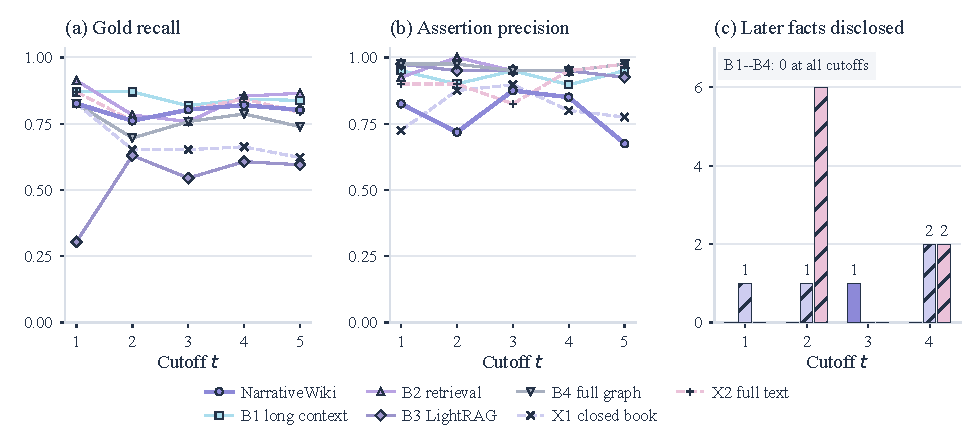
\includegraphics[width=\textwidth]{figures/f2-cutoff-anne.pdf}
\caption{Original text: recall and precision at each cutoff (lines), and counts of assessed
later facts disclosed (bars). Dashed lines denote the X1 and X2 diagnostics. B1--B4 have zero observed
disclosures at every cutoff. Disclosure denominators are $|\Ft|=88,65,45,22$ at
$t=1,\ldots,4$; disclosure is undefined at $t=5$.}
\label{fig:cutoffplot}
\end{figure*}


Tables~\ref{tab:full-results} (original text) and~\ref{tab:decon-cells} (treated text) report the individual cells underlying the means in
Table~\ref{tab:main}; Figure~\ref{fig:cutoffplot} plots them. Long-context recall is
approximately stable across cutoffs. \sys has its highest recall on the first book, where it
matches the closed-book diagnostic, and its lowest at $t=2$. Closed-book recall declines from
the first book to the fifth. LightRAG's low recall at $t=1$ accompanies retrieved context
concentrated on the opening chapters. With only 40 sampled atoms per cell, the precision
results do not establish a trend across cutoffs. Every reported model call used the shared
generator. Table~\ref{tab:stats} gives the mean, standard deviation, median, minimum, and
maximum across cutoffs; Table~\ref{tab:paired} reports the same summaries for the paired
differences discussed in Section~\ref{sec:results}.

% Appendix: analyses that support Section 6 and did not fit in it.
\section{Additional Results}
\label{app:additional}

\begin{table}[t]
\centering\small
\setlength{\tabcolsep}{3pt}
\begin{tabular}{@{}lccc@{}}
\toprule
 & \nwhead{Cutoffs} & \nwhead{M1, M3,} & \nwhead{M8} \\
 & \nwhead{built} & \nwhead{M4} &  \\
\midrule
B1, B2, \sys & 1--5 & labeled & labeled \\
\quad on prefix indexes & 1--4 & labeled & labeled \\
B3, B4, X2 & 1--5 & labeled & labeled \\
X1 (cites nothing) & 1--5 & labeled & -- \\
\sys, first build & 1--5 & labeled & labeled \\
\quad from a prefix & 2, 3 & labeled & -- \\
\bottomrule
\end{tabular}
\caption{What was built and labeled. Every label is by an LLM annotator
(Section~\ref{sec:setup}).}
\label{tab:coverage}
\end{table}

\paragraph{Coverage of the evaluation.}
Table~\ref{tab:coverage} lists the available builds and labels. B4's aggregate results are
included in Table~\ref{tab:main}, with per-cutoff values below. The first build of \sys
and its prefix variants support the analyses in Sections~\ref{sec:results-quality}
and~\ref{sec:results-scope}.

\begin{table}[t]
\centering\small
\setlength{\tabcolsep}{3pt}
\begin{tabular}{@{}lrr@{}}
\toprule
\nwhead{Seeded sentence} & \nwhead{Retrieved} & \nwhead{Rate} \\
\midrule
Gold claim verbatim & 220 & 1.000 \\
Paraphrase, names the character & 186 & 0.845 \\
Paraphrase, pronoun, own page & 169 & 0.768 \\
Paraphrase, pronoun, other page & 68 & \cellcolor{nwhighpink}\best{0.309} \\
Implying, names the character & 157 & 0.714 \\
Implying, pronoun, own page & 137 & 0.623 \\
Implying, pronoun, other page & 78 & \cellcolor{nwhighpink}\best{0.355} \\
\bottomrule
\end{tabular}
\caption{Recall of the disclosure candidate search on seeded disclosures: 220 fact-by-cutoff
units ($t=1..4$), one paraphrase and one implying sentence per later fact, each checked to
establish its fact. Bold magenta cells mark the lowest rate of each kind.}
\label{tab:seeds}
\end{table}

\paragraph{What the disclosure search retrieves.}
Disclosure judgments are limited to sentences returned by candidate search. We therefore
test retrieval on seeded sentences with known disclosures (Table~\ref{tab:seeds}). Search
retrieves every verbatim claim, about 85\% of named paraphrases and about 70\% of named
implications; pronouns on another character's page reduce retrieval to roughly one third.
The corresponding rates are \res{SEED-direct} for verbatim claims,
\res{SEED-para} and \res{SEED-para-pron} for paraphrases, and
\res{SEED-oblique} and \res{SEED-oblique-pron} for implications.
Search produced \res{M4-cand-anne-B5} candidate sentences for \sys,
\res{M4-cand-anne-B1} for B1 and \res{M4-cand-anne-all} across systems and builds.
A lexical-screen hit on X2 exposed an unmatched phrase (``to marry''); after correcting
the matcher, \res{M4-anne-reread} sentences were reassessed. Of 224 eligible claims passed
through the same search, 14 became candidates for a later fact about the same character.
Retrieval alone does not count as disclosure.

The annotator model wrote and checked each fixture for its subject, event and object,
independently of whether search retrieved it. An earlier fixture version, in which many
implications did not establish their target fact, had retrieval of approximately one
quarter and is released alongside the validated version. No second reader validated
the fixtures. The search-independent checks of Section~\ref{sec:results-main} also have
limits: lexical screening detects only new names, while zero later-volume assertions in
a sample of approximately 160 atoms gives limited evidence about rare disclosures.
Overlapping cutoff wikis and clustering within pages reduce the effective sample size.

\begin{table}[t]
\centering\small
\setlength{\tabcolsep}{2.3pt}
\begin{tabular}{@{}l@{\hspace{2pt}}rrrrr@{}}
\toprule
 & \nwhead{Share} & \nwhead{$n$} & \nwhead{Page} & \nwhead{Atom} & \nwhead{Suff.} \\
\midrule
Character pages, cast & 0.206 & 35 & 31 & 31 & 14 \\
Character pages, other & 0.171 & 29 & 22 & 24 & 15 \\
Relationship pages & \cellcolor{nwhighlavender}\best{0.463} & 102 & \cellcolor{nwhighpink}\best{72} & \best{99} & 60 \\
Codex pages & 0.057 & 11 & 11 & 11 & 2 \\
Timeline & 0.090 & 22 & 21 & 21 & 11 \\
Index & 0.012 & 0 & -- & -- & -- \\
\midrule
\sys, all pages & 1.000 & 199 & 157 & 186 & 102 \\
B1 (cast pages only) & 1.000 & 199 & 185 & 185 & 131 \\
B2 (cast pages only) & 1.000 & 199 & 191 & 191 & 154 \\
\bottomrule
\end{tabular}
\caption{The precision samples by kind of page, pooled over cutoffs. Share: of the system's
assertions on that kind of page; $n$: sampled atoms; Page and Atom: supported on the page that
prints them (relationship pages under the pair rule of Appendix~\ref{app:annotation}), and as
statements; Suff.: established by their own cited paragraphs. Lavender marks the largest
kind of page; magenta its page-context support, which falls short of its assertions true as
statements.}
\label{tab:kinds}
\end{table}

\begin{figure*}[t]
\centering
\resizebox{\textwidth}{!}{% F8 (v3, full width): context collapse (RQ4) and identity dependence (RQ5). Coordinates are typed
% from tab:kinds (Appendix G; counts of 199 sampled original-text assertions per system) and from
% tab:identity (page counts per cutoff); printed rates are \res keys. Re-type if they change.
\begin{tikzpicture}[x=1cm, y=0.82cm, font=\figfont,
  ptitle/.style={anchor=north west, font=\figfont\bfseries, text=nwink, inner sep=0pt},
  tick/.style={font=\fontsize{5.6}{6}\selectfont, text=nwSlate},
  val/.style={font=\fontsize{5.4}{6}\selectfont, text=nwink, inner sep=1pt}]

% ------------------------------------------------------------- (a) statement truth vs page support
\begin{scope}[shift={(2.6,0)}]
\node[ptitle] at (-2.6,3.3) {(a) Precision of sampled assertions: true as a statement vs.\ supported on its page};
\def\W{5.0}
\foreach \v/\l in {0/0, 0.5/0.5, 0.75/0.75, 1/1}{\draw[nwgrid] (\v*\W,-0.05) -- (\v*\W,2.95); \node[tick] at (\v*\W,-0.2) {\l};}
% \kind{y}{label}{statement}{page}{n label}
\newcommand{\kind}[5]{\node[tick, anchor=east, text=nwink, align=right] at (-0.05,#1) {#2};
  \fill[nwSlate] (0,#1+0.02) rectangle (#3*\W,#1+0.13);
  \fill[nwCyan] (0,#1-0.13) rectangle (#4*\W,#1-0.02);
  \node[val, anchor=west] at (\W+0.05,#1) {#5};}
\kind{2.8}{Relationship pages (46\%)}{0.971}{0.706}{99 / 72 of 102}
\fill[nwLav!55] (0.706*\W,2.67) rectangle (0.971*\W,2.78);
\node[val, text=nwViolet] at (0.84*\W,2.55) {gap: true lines on pair pages};
\kind{2.15}{Cast character pages (21\%)}{0.886}{0.886}{31 / 31 of 35}
\kind{1.75}{Other character pages (17\%)}{0.828}{0.759}{24 / 22 of 29}
\kind{1.35}{Timeline pages (9\%)}{0.955}{0.955}{21 / 21 of 22}
\kind{0.95}{Codex pages (6\%)}{1.000}{1.000}{11 / 11 of 11}
\draw[nwgrid, densely dotted] (-2.6,0.72) -- (\W+1.3,0.72);
\kind{0.5}{\sys, all pages}{0.935}{0.789}{186 / 157 of 199}
\kind{0.1}{B1, cast pages}{0.930}{0.930}{185 / 185 of 199}
\fill[nwSlate] (0,-0.55) rectangle (0.15,-0.45); \node[tick, anchor=west] at (0.15,-0.5) {true as a statement};
\fill[nwCyan] (1.6,-0.55) rectangle (1.75,-0.45); \node[tick, anchor=west] at (1.75,-0.5) {supported on the page (scene rule)};
\end{scope}

% ------------------------------------------------------------- (b) identity dependence by cutoff
\begin{scope}[shift={(10.45,0)}]
\node[ptitle] at (-0.6,3.3) {(b) Character pages vs.\ a prefix-built index};
\def\W{4.4}
\foreach \v/\l in {0/0, 0.5/0.5, 1/1}{\draw[nwgrid] (\v*\W,0.1) -- (\v*\W,2.95); \node[tick] at (\v*\W,-0.05) {\l};}
% \idbar{y}{t}{same}{alias}{regrouped}{absent}{pages}{label}
\newcommand{\idbar}[8]{\node[tick, anchor=east, text=nwink] at (-0.05,#1) {$t{=}#2$};
  \pgfmathsetmacro{\ia}{#3/#7*\W}\pgfmathsetmacro{\ib}{(#3+#4)/#7*\W}\pgfmathsetmacro{\ic}{(#3+#4+#5)/#7*\W}
  \fill[nwLight] (0,#1-0.17) rectangle (\ia,#1+0.17);
  \fill[nwLav] (\ia,#1-0.17) rectangle (\ib,#1+0.17);
  \fill[nwMagenta!55] (\ib,#1-0.17) rectangle (\ic,#1+0.17);
  \fill[nwMagenta] (\ic,#1-0.17) rectangle (\W,#1+0.17);
  \node[val, anchor=west] at (\W+0.05,#1) {#8};}
\idbar{2.6}{1}{36}{10}{4}{9}{59}{\res{ID-anne-t1-rate}}
\idbar{1.95}{2}{87}{13}{7}{10}{117}{\respt{ID-anne-t2}}
\idbar{1.3}{3}{137}{9}{4}{8}{158}{\respt{ID-anne-t3}}
\idbar{0.65}{4}{174}{7}{5}{5}{191}{\res{ID-anne-t4-rate}}
\fill[nwLight] (0,-0.38) rectangle (0.15,-0.28); \node[tick, anchor=west] at (0.15,-0.33) {same};
\fill[nwLav] (0.85,-0.38) rectangle (1.0,-0.28); \node[tick, anchor=west] at (1.0,-0.33) {alias only};
\fill[nwMagenta!55] (1.95,-0.38) rectangle (2.1,-0.28); \node[tick, anchor=west] at (2.1,-0.33) {regrouped};
\fill[nwMagenta] (3.15,-0.38) rectangle (3.3,-0.28); \node[tick, anchor=west] at (3.3,-0.33) {absent};
\node[tick, anchor=west, text=nwink] at (-0.6,-0.65) {Prefix-index wikis: pooled recall \res{PX-anne-M1-pooled}, as the full build.};
\end{scope}
\end{tikzpicture}
}
\caption{Context collapse (RQ4) and identity dependence (RQ5), original text. (a) On
relationship pages nearly every line is true, but a quarter sit under a pair that shares no
episode; on cast pages the two measures agree. (b) \sys's character pages against an entity
index discovered from volumes $1..t$; the printed rate is the share that differ.}
\label{fig:collapse}
\end{figure*}

\paragraph{Matched and whole-artifact populations.}
Table~\ref{tab:kinds} separates sampled assertions by page type. The comparison systems
publish only cast character pages; on this matched population, 31 of \sys's 35 sampled
atoms are supported. This small subsample does not support a precise comparison with the
baselines, and no equivalence test is reported. Of \sys's 42 page-context negatives, 30
occur on relationship pages; 27 of those 30 are supported as statements but placed under
a pair that shares no episode of the scene.

For every \sys page type, observed citation sufficiency is below the overall values of
B1 and B2. Cited paragraphs establish 14 of 35 atoms on cast pages, 60 of 102 on
relationship pages and 11 of 22 on the timeline. Timeline lines can carry up to four
paragraphs selected to support a chapter-level summary.


\begin{table*}[t]
\centering\small
\setlength{\tabcolsep}{6pt}
\begin{tabular}{@{}cllllr@{}}
\toprule
\nwhead{$t$} & \nwhead{Recall} & \nwhead{Precision} & \nwhead{Citation} & \nwhead{Disclosed} & \nwhead{Assertions} \\
\midrule
1 & \cellcolor{nwhighcyan}\best{\res{M1-anne-t1-B4}} & \res{M3-anne-t1-B4} & \res{M8-anne-t1-B4} & \res{M4-anne-t1-B4} & \res{N-anne-t1-B4} \\
2 & \cellcolor{nwhighpink}\best{\res{M1-anne-t2-B4}} & \res{M3-anne-t2-B4} & \res{M8-anne-t2-B4} & \res{M4-anne-t2-B4} & \res{N-anne-t2-B4} \\
3 & \res{M1-anne-t3-B4} & \res{M3-anne-t3-B4} & \res{M8-anne-t3-B4} & \res{M4-anne-t3-B4} & \res{N-anne-t3-B4} \\
4 & \res{M1-anne-t4-B4} & \res{M3-anne-t4-B4} & \res{M8-anne-t4-B4} & \res{M4-anne-t4-B4} & \res{N-anne-t4-B4} \\
5 & \res{M1-anne-t5-B4} & \res{M3-anne-t5-B4} & \res{M8-anne-t5-B4} & -- & \res{N-anne-t5-B4} \\
\bottomrule
\end{tabular}
\caption{B4, the graph baseline (the full graph, filtered at retrieval time), at every cutoff. Columns as in
Table~\ref{tab:full-results}; Claude finalized the citation labels at every cutoff.
Bold marks the highest and lowest recall, highlighted in cyan and pink, respectively.}
\label{tab:b4}
\end{table*}

\paragraph{The graph baseline (B4).}
Table~\ref{tab:b4} reports B4 at every cutoff, using the reported \sys graph.
Mean recall is \respt{M1-anne-avg-B4}, versus \respt{M1-anne-avg-B5} for \sys:
lower at four cutoffs and equal at one. Mean precision is \respt{M3-anne-avg-B4}.
No assessed later fact was disclosed (\res{M4-anne-total-B4}); B4 publishes
\res{ND-anne-avg-B4} distinct assertions per cutoff and has \res{SCREEN-anne-B4}
lexical-screen hit, the same expanded page title found in the prefix baselines.

B4 generates cast character pages from a budgeted selection of retrieved graph facts;
\sys renders all eligible facts and also publishes relationship, codex and timeline
pages. B4's higher precision, together with the 30 relationship-page negatives among
\sys's 42 page-context negatives, suggests that publication context contributes to
the gap in Table~\ref{tab:main}. This comparison does not isolate context from selection
and generation.

B4's cited paragraphs suffice for \respt{M8-anne-avg-B4} of sampled assertions, and none
of its 200 sampled citations is judged wholly unrelated to the assertion.
The corresponding whole-artifact value for \sys is \respt{M8-anne-avg-B5};
on character pages it is \res{M8K-anne-char-B5}, versus \res{M8K-anne-char-B4} for B4.
These observations show that evidence stored in the common graph can support generated
assertions, while \sys's evidence selection or attachment is less reliable.

\begin{table}[t]
\centering\small
\setlength{\tabcolsep}{3pt}
\begin{tabular}{@{}lrr@{}}
\toprule
 & \nwhead{$t=2$} & \nwhead{$t=3$} \\
\midrule
Pages, full build & \res{A1-t2-pages-full} & \res{A1-t3-pages-full} \\
Pages, prefix build & \res{A1-t2-pages-prefix} & \res{A1-t3-pages-prefix} \\
In both builds & \res{A1-t2-shared} & \res{A1-t3-shared} \\
\quad same title & 100 & 145 \\
\quad same alias list & 80 & 128 \\
\quad alias not in $\Dt$ (full) & 0 & 0 \\
In one build only & \res{A1-t2-onesided} & \res{A1-t3-onesided} \\
\quad later-anchored & \cellcolor{nwhighpink}\best{\res{A1-t2-classes-anchored}} & \cellcolor{nwhighpink}\best{\res{A1-t3-classes-anchored}} \\
\quad second page, same person & \res{A1-t2-classes-duplicate} & \res{A1-t3-classes-duplicate} \\
\quad same person, new address & \res{A1-t2-classes-renamed} & \res{A1-t3-classes-renamed} \\
\quad minor entity & \res{A1-t2-classes-selection} & \res{A1-t3-classes-selection} \\
\quad stating a later fact & 0 & 0 \\
\midrule
Recall, prefix build & \res{A1-t2-M1-prefix} & \res{A1-t3-M1-prefix} \\
Recall, full build & \cellcolor{nwhighcyan}\best{\res{A1-t2-M1-full}} & \cellcolor{nwhighcyan}\best{\res{A1-t3-M1-full}} \\
Precision, prefix build & \cellcolor{nwhighcyan}\best{\res{A1-t2-M3-prefix}} & \cellcolor{nwhighcyan}\best{\res{A1-t3-M3-prefix}} \\
Precision, full build & \res{A1-t2-M3-full} & \res{A1-t3-M3-full} \\
Later facts disclosed & 0/65 & 0/45 \\
Prefix build tokens (M) & \res{TOK-A1-t2-prefix} & \res{TOK-A1-t3-prefix} \\
\bottomrule
\end{tabular}
\caption{Construction scope (character pages), first build of \sys: built from volumes
$1..t$ alone (prefix) against the same cutoff of its five-volume build (full;
\res{TOK-anne-first-text} once, for all cutoffs). Precision is under the pair rule of Appendix~\ref{app:annotation}.
Disclosure counts are identical in the two builds; tokens are input / output, in millions.
Bold magenta cells mark later-anchored pages; bold cyan cells mark the higher of the two builds
on recall and precision.}
\label{tab:scope}
\end{table}

\begin{table*}[t]
\centering\small
\setlength{\tabcolsep}{4pt}
\begin{tabular}{@{}rrrrrrlll@{}}
\toprule
\nwhead{$t$} & \nwhead{Pages} & \nwhead{Same} & \nwhead{Alias} & \nwhead{Regrouped} & \nwhead{Absent} & \nwhead{Identity dependence} & \nwhead{Regrouped or absent} & \nwhead{Mentions} \\
\midrule
1 & 59 & 36 & 10 & 4 & 9 & \cellcolor{nwhighpink}\best{\res{ID-anne-t1}} & \cellcolor{nwhighpink}\best{\res{ID-anne-strict-t1}} & \cellcolor{nwhighpink}\best{\res{ID-anne-mentions-t1}} \\
2 & 117 & 87 & 13 & 7 & 10 & \res{ID-anne-t2} & \res{ID-anne-strict-t2} & \res{ID-anne-mentions-t2} \\
3 & 158 & 137 & 9 & 4 & 8 & \res{ID-anne-t3} & \res{ID-anne-strict-t3} & \res{ID-anne-mentions-t3} \\
4 & 191 & 174 & 7 & 5 & 5 & \res{ID-anne-t4} & \res{ID-anne-strict-t4} & \res{ID-anne-mentions-t4} \\
\bottomrule
\end{tabular}
\caption{Identity dependence of the reported \sys on the original text. Each character page of the
five-volume build at cutoff $t$ is compared with the entity index built from volumes $1..t$ alone.
\emph{Same}: a prefix-built character has exactly its set of names seen by $t$. \emph{Alias}: one
counterpart, with a name linked in one build only. \emph{Regrouped}: names that one build gives
one character the other gives two. \emph{Absent}: no prefix-built entity carries any of its names.
\emph{Mentions}: character mentions in volumes $1..t$ under the prefix index, as a share of the
full build's. One run per index, so model variance is inside the differences.
Bold magenta cells mark the cutoff where identity dependence is largest.}
\label{tab:identity}
\end{table*}

\paragraph{Identity dependence.}
Table~\ref{tab:identity} reports the measure defined in Section~\ref{sec:results-scope};
its mean is \res{ID-anne-mean}. Every prefix-built character has a counterpart in the
full build, although counterpart existence does not imply identical alias grouping.

Some differences arise deterministically during candidate mining. Of the full build's
candidates first occurring by $t$, \res{G19-anne-lost} are absent from prefix mining
($t=1..4$). Most, \res{G19-anne-few}, occur fewer than three times in the prefix and
reach the miner's frequency threshold only with later occurrences. The remaining
\res{G19-anne-ratio} fail a separate rule: a single capitalized word must stand alone
in at least three quarters of its occurrences in some volume. Bare \emph{Gilbert}
appears alone in 62 of 113 book-one occurrences; the other 51 are in
\emph{Gilbert Blythe}. Prefix mining therefore omits the alias, while later volumes
allow the full build to retain it. Disabling this rule admits \res{G19-anne-off}
additional full-build candidates, mostly sentence-initial words. We retain the reported
rule because changing it would alter the evaluated index.

Pages absent from the prefix index at $t=1$ include \texttt{walter}, \texttt{jerry}
and \texttt{marshall}, discussed below, and Anne's mother, whose full name occurs once
in book one. The four prefix indexes use \res{TOK-ID-anne}, including
\res{TOK-ID-anne-new} in calls absent from the full build's cache.
The measure captures entity-index sensitivity to construction scope; wiki outcomes
on these indexes appear in Table~\ref{tab:prefixv2}.

\begin{table*}[t]
\centering\small
\begin{tabular}{@{}llrrrr@{}}
\toprule
 & \nwhead{Build} & \nwhead{$t=1$} & \nwhead{$t=2$} & \nwhead{$t=3$} & \nwhead{$t=4$} \\
\midrule
Character pages & full & \res{PX-anne-t1-pages-full} & \res{PX-anne-t2-pages-full} & \res{PX-anne-t3-pages-full} & \res{PX-anne-t4-pages-full} \\
 & prefix & \res{PX-anne-t1-pages} & \res{PX-anne-t2-pages} & \res{PX-anne-t3-pages} & \res{PX-anne-t4-pages} \\
Recall & full & \res{M1-anne-t1-B5} & \res{M1-anne-t2-B5} & \res{M1-anne-t3-B5} & \cellcolor{nwhighcyan}\best{\res{M1-anne-t4-B5}} \\
 & prefix & \res{PX-anne-t1-M1} & \res{PX-anne-t2-M1} & \cellcolor{nwhighcyan}\best{\res{PX-anne-t3-M1}} & \res{PX-anne-t4-M1} \\
Precision & full & \res{M3-anne-t1-B5} & \res{M3-anne-t2-B5} & \res{M3-anne-t3-B5} & \cellcolor{nwhighcyan}\best{\res{M3-anne-t4-B5}} \\
 & prefix & \cellcolor{nwhighcyan}\best{\res{PX-anne-t1-M3}} & \cellcolor{nwhighcyan}\best{\res{PX-anne-t2-M3}} & \res{PX-anne-t3-M3} & \res{PX-anne-t4-M3} \\
Citation sufficiency & full & \res{M8-anne-t1-B5} & \cellcolor{nwhighcyan}\best{\res{M8-anne-t2-B5}} & \res{M8-anne-t3-B5} & \res{M8-anne-t4-B5} \\
 & prefix & \cellcolor{nwhighcyan}\best{\res{PX-anne-t1-M8}} & \res{PX-anne-t2-M8} & \cellcolor{nwhighcyan}\best{\res{PX-anne-t3-M8}} & \cellcolor{nwhighcyan}\best{\res{PX-anne-t4-M8}} \\
Later facts disclosed & full & \res{M4-anne-t1-B5} & \res{M4-anne-t2-B5} & \cellcolor{nwhighpink}\best{\res{M4-anne-t3-B5}} & \res{M4-anne-t4-B5} \\
 & prefix & \res{PX-anne-t1-M4} & \res{PX-anne-t2-M4} & \cellcolor{nwhighcyan}\best{\res{PX-anne-t3-M4}} & \res{PX-anne-t4-M4} \\
Assertions & full & \res{N-anne-t1-B5} & \res{N-anne-t2-B5} & \res{N-anne-t3-B5} & \res{N-anne-t4-B5} \\
 & prefix & \res{PX-anne-t1-N} & \res{PX-anne-t2-N} & \res{PX-anne-t3-N} & \res{PX-anne-t4-N} \\
\midrule
Tokens, in / out (M) & prefix & \res{PX-anne-t1-TOK} & \res{PX-anne-t2-TOK} & \res{PX-anne-t3-TOK} & \res{PX-anne-t4-TOK} \\
\bottomrule
\end{tabular}
\caption{The reported \sys built on entity indexes discovered from the prefix (\emph{prefix}: one build
per cutoff, every stage on volumes $1..t$) against the same cutoff of its five-volume build (\emph{full}).
Metrics as in Table~\ref{tab:full-results}; precision is on a different sample of 40 assertions in each
build. The prefix builds received a single LLM labeling pass; the full build's labels were
finalized by Claude Opus~5.5 (Appendix~\ref{app:annotation}). The full
build's tokens, for all five cutoffs at once, are in Table~\ref{tab:efficiency}.
Bold cyan cells mark the higher rate where the builds differ; bold magenta cells mark non-zero
disclosure counts.}
\label{tab:prefixv2}
\end{table*}

\paragraph{Wikis built on the prefix indexes.}
Table~\ref{tab:prefixv2} evaluates the complete reported pipeline on each prefix
$t=1..4$, using that prefix's entity index. Pooled recall is
\res{PX-anne-M1-pooled} gold-fact assessments for the prefix builds and
\res{PX-anne-M1-pooled-full} for the full build. Per-cutoff differences comprise one
to three facts in either direction: prefix builds lose a minor character's trait
and gain an office or prize omitted by the full build. Pooled precision is
\res{PX-anne-M3-pooled}, versus \res{PX-anne-M3-pooled-full}, on different samples.
Citation sufficiency is \res{PX-anne-M8-pooled}, versus
\res{PX-anne-M8-pooled-full}, using different samples with labels finalized by Claude.

Neither build states a later fact. Both contain the same implied disclosure at $t=3$,
the bridesmaid relation inverted from eligible text. Prefix builds publish fewer
character pages at early cutoffs: \texttt{walter} and \texttt{jerry}, retained by the
full build at every cutoff because of book-five characters, never appear in prefix
builds; \texttt{marshall}, from book four, appears only at $t=4$.
Prefix-specific discovery avoids using later text in entity construction while retaining
the observed pooled gold recall. This is not evidence of equivalence on all outcomes:
the approach requires a build per cutoff, and the four prefix builds together use more
tokens than the single full build.

\paragraph{Construction scope.}
Table~\ref{tab:scope} compares prefix and full graphs made with first-build code;
this complete graph comparison was not repeated for the reported build.
The pooled recall difference is \res{A1-dM1}, with seven discordant facts; the precision
difference is \res{A1-dM3}, using separate samples. These comparisons cannot isolate
construction-scope effects from differences in entity indexes and model runs.

At $t=2$, later-anchored pages include \texttt{walter} (Walter Blythe of book five,
127 of the entity's 130 mentions, but an early page describing Anne's father);
\texttt{di} (Di Blythe, with an early duplicate page for Diana Barry under a nickname
used once in the first two books); \texttt{mary} (Mary Vance, showing the twins' mother);
\texttt{jerry} (Jerry Meredith, merging a book-one hired boy with a book-two agent);
and \texttt{marshall}, \texttt{baxter} and \texttt{sam}.
An entity-merge audit flags \res{A1-merge-full} entities in the full build and
\res{A1-merge-prefix} in a volume-one build.

Shared pages have identical titles and no full-build alias absent from $\Dt$.
Relation lines differ in both directions: at $t=2$, 54 occur in both builds,
93 only in the full build and 68 only in the prefix build. Separate runs and
entity lists prevent attributing these differences solely to later volumes.
Prose on shared pages was not compared.

\paragraph{Later-anchored entities in the reported build.}
The reported build adjudicates bare names against fuller forms first appearing later,
and assigns shared first names volume by volume to the locally dominant full name.
Its \texttt{walter} entity now contains only Anne's father (three mentions), with
Walter Blythe appearing separately from book five.

A separate screen flags character-page entities with at least ten mentions and
at least four fifths occurring after the cutoff: \res{LATE-anne-t2} at $t=2$ and
\res{LATE-anne-t3} at $t=3$. At $t=2$, these are \texttt{susan} (3 of 204 mentions
by book two; an empty page dominated by Susan Baker of books four and five);
\texttt{sam} (2 of 10, with prose saying ``Sam does not appear in the story provided'');
\texttt{joseph} (5 of 54, an early pupil's uncle under an entity later dominated by
others); \texttt{jerry-corcoran} (6 of 120, correctly described at $t=2$ but later
absorbing Jerry Meredith); and \texttt{stella-maynard} and \texttt{billy-andrews},
correctly resolved people introduced early. This screen identifies entities dominated
by later mentions. It neither establishes dependence for every flagged page nor
determines what a prefix build would publish instead.

\begin{table}[t]
\centering\small
\setlength{\tabcolsep}{4pt}
\begin{tabular}{@{}lrrr@{}}
\toprule
\nwhead{Stage} & \nwhead{Calls} & \nwhead{Input} & \nwhead{Output} \\
\midrule
Entity discovery & \res{T5-gazetteer-calls} & \res{T5-gazetteer-in} & \res{T5-gazetteer-out} \\
Chapter pass & \res{T5-scenes-calls} & \res{T5-scenes-in} & \cellcolor{nwhighviolet}\best{\res{T5-scenes-out}} \\
Mention pass & \cellcolor{nwhighviolet}\best{\res{T5-extract-calls}} & \cellcolor{nwhighviolet}\best{\res{T5-extract-in}} & \res{T5-extract-out} \\
Long-context pass & \res{T5-infobox-calls} & \res{T5-infobox-in} & \res{T5-infobox-out} \\
Arbitration & \res{T5-graph-calls} & \res{T5-graph-in} & \res{T5-graph-out} \\
Verification & \res{T5-verify-calls} & \res{T5-verify-in} & \res{T5-verify-out} \\
Prose & \res{T5-synth-calls} & \res{T5-synth-in} & \res{T5-synth-out} \\
Shared-page summaries & \res{T5-site-calls} & \res{T5-site-in} & \res{T5-site-out} \\
\midrule
Total, reported runs & \res{T5-total-calls} & \res{T5-total-in} & \res{T5-total-out} \\
Rebuild from cache & 0 & 0 & 0 \\
\bottomrule
\end{tabular}
\caption{Size of the reported \sys build for all five cutoffs, including verification
rechecks after one re-extraction: model calls, and input and output tokens in millions. Every call of the build is counted, whether or not the
provider served it at a discount, so the token column of Table~\ref{tab:main} is comparable
across systems. A rebuild from the call cache sends nothing. Ingestion, assembly and linking
make no model call. Bold violet cells identify the stage consuming the most resources in
each column.}
\label{tab:efficiency}
\end{table}

\paragraph{Cost.}
Table~\ref{tab:efficiency} breaks down model use by stage; extraction dominates.
Prose and shared-page summaries are generated once per distinct filtered fact set,
across all five cutoffs, and included in the total. Verification includes rechecks
after one re-extraction, so its count slightly exceeds a cold build from an empty cache.
The first build used \res{TOK-anne-first-text} under the same accounting.
B4 adds \res{TOK-anne-B4} million tokens (input / output) of page generation to the
graph it shares with \sys; latency, hardware and the local evaluation models are not
costed for any system.

Long-context input grows with the prefix (\res{COST-anne-B1-input} tokens at $t=1..5$),
which is sent once per page. The all-cutoff \sys build uses
\res{COST-anne-B5-input} input tokens. LightRAG's \res{TOK-anne-B3} million tokens
(input / output) comprise \res{TOK-anne-B3-index} for five incremental indexes
and \res{TOK-anne-B3-pages} for page generation. Prefix retrieval indexes use local
embeddings and BM25, so its \res{TOK-anne-B2} million tokens cover page generation.
The closed-book diagnostic uses \res{TOK-anne-X1}.

\paragraph{Verification.}
At audit, the verifier had marked \res{VERIFY-unsupported} facts unsupported by their
cited evidence; these facts are withheld. Table~\ref{tab:efficiency} counts verification
calls rather than distinct facts. On a challenge set of \res{M12-n} items created by
minimal substitutions in source-verified facts, the verifier accepted
\res{M12-false-admit} labeled unsupported candidates and rejected
\res{M12-false-reject} labeled supported ones (Appendix~\ref{app:evaluator}).
This synthetic challenge does not establish performance on naturally occurring
extraction errors.

\paragraph{Facts \sys misses.}
At $t=5$, \sys misses \res{M1-anne-miss-t5} of the \res{T1-anne-gold-t5} gold facts;
B1 or B2 conveys \res{M1-anne-miss-t5-prefix} of those omissions. Examples include
Gilbert's teaching appointment at White Sands and Cooper Prize, Diana's role as
improvement-society treasurer, Rilla's position as the youngest Blythe child,
Leslie's mother's pressure to marry, Mr.\ Phillips's interest in Prissy Andrews,
and Paul Irving's place of origin. Conversely, four facts are conveyed by \sys
but neither B1 nor B2: Anne's fictional heroine, her mother's letters, Gilbert's
boat rescue of Anne and Walter's hatred of a schoolmate. Four facts are conveyed
by none of these three systems.

\paragraph{Typical errors.}
\sys still merges namesakes. Priscilla Grant's page lists the book-one schoolgirl
``Prissy Andrews'' as an alias. The \texttt{james-a} page joins Mr.\ Harrison of
book two, who also has a separate page, with a deceased James of book three and
a book-four sailor. A duplicate page for Anne, \texttt{shirley}, also absorbs her
son Shirley at $t=5$ (``the little brown boy'').

Other errors include a remark by Mrs.\ Barry attributed to Marilla, an inverted
relationship (Section~\ref{sec:results-main}), intervals persisting beyond their
validity and an exhibition prize labeled ``Fought in''. Generated commentary
about the input can reach pages: one subject ``does not appear in the story
provided'', and 5 of the 341 non-timeline pages at $t=4$ retain source-line keys
(``[R3, R4, S1, S4]''; Table~\ref{tab:qual-diff}).
Two first-build errors were not observed in the reported build: Anne's mother's
death specified as ``of yellow fever'', beyond the text, and a merger of two men
named George.

B1 and X2 also misattribute biographies: at $t=5$, both place one man's courtship
and marriage on another man's page. The closed-book diagnostic imports material
outside the five-book corpus, describing Anne's years at ``Windy Willows''.

\paragraph{Uncertain disclosure verdicts.}
\begin{table}[t]
\centering\small
\setlength{\tabcolsep}{5pt}
\begin{tabular}{@{}lrr@{}}
\toprule
\nwhead{System} & \nwhead{Original} & \nwhead{Treated} \\
\midrule
B1 & \res{M4U-anne-B1} & \res{M4U-annedecon-B1} \\
B2 & \res{M4U-anne-B2} & \res{M4U-annedecon-B2} \\
B3 & \res{M4U-anne-B3} & \res{M4U-annedecon-B3} \\
B4 & \res{M4U-anne-B4} & \res{M4U-annedecon-B4} \\
B5 (\sys) & \res{M4U-anne-B5} & \res{M4U-annedecon-B5} \\
X1 & \res{M4U-anne-X1} & \res{M4U-annedecon-X1} \\
X2 & \res{M4U-anne-X2} & \res{M4U-annedecon-X2} \\
\bottomrule
\end{tabular}
\caption{Confirmed unique subject facts disclosed, over unique assessed subject facts.
The unit is (character, claim, reveal volume): repeated cutoffs collapse, while reciprocal
character facts remain distinct. These are not independent event or error counts.}
\label{tab:disclosure-units}
\end{table}

System-level uncertain counts at $t=1..4$ are \res{M4-anne-uncertain}.
For \sys, four verdicts arise from one relation line between Anne and Gilbert,
``Romantically involved with --- harbors romantic feelings for her''.
The interval opens in book one from a friend's report that Gilbert kept a rose
Anne dropped. Assessed at $t=1$ and $t=2$ against two later facts about the
couple, the line yields four uncertain judgments because it could suggest
their book-four marriage.

\paragraph{Unique facts and error mechanisms.}
Table~\ref{tab:disclosure-units} collapses repeated fact--cutoff assessments to unique
subject facts. On the original text, \sys's confirmed disclosure concerns one fact from
one inverted-bridesmaid error. On the treated text, its four confirmed assessments cover
two reciprocal marriage facts at two cutoffs, arising from a single prediction-to-marriage
failure mechanism. B4's two treated assessments concern those same reciprocal facts.
These witness-based descriptions do not establish that every output error has been found
or that error mechanisms are independent. Grouping systems by information available to
page generation includes B4 alongside B1--B3 and B5: together they have
\res{M4-anne-total-cut} original-text assessments, or
\res{M4-anne-total-cut-incl} including uncertain verdicts.

\begin{table}[t]
\centering\small
\setlength{\tabcolsep}{3pt}
\begin{tabular}{@{}lrr@{}}
\toprule
 & \nwhead{First} & \nwhead{Reported} \\
\midrule
Recall & \cellcolor{nwhighcyan}\best{\res{REV-M1-first}} & \respt{M1-anne-avg-B5} \\
Precision, scene rule & \res{REV-M3-first} & \cellcolor{nwhighcyan}\best{\respt{M3-anne-avg-B5}} \\
Precision, line rule & \res{REV-M3L-first} & \cellcolor{nwhighcyan}\best{\res{REV-M3L}} \\
True as statements & \cellcolor{nwhighcyan}\best{\res{REV-M3A-first}} & \res{REV-M3A} \\
Citation sufficiency & \res{REV-M8-first} & \cellcolor{nwhighcyan}\best{\respt{M8-anne-avg-B5}} \\
With a paragraph citation (all) & \res{REV-CITE-first} & \cellcolor{nwhighcyan}\best{\res{CITE-anne-B5}} \\
Later facts disclosed & \best{\res{REV-M4-first}} & \cellcolor{nwhighpink}\res{M4-anne-total-B5} \\
Lexical screen hits & \res{REV-SCREEN-first} & \cellcolor{nwhighcyan}\best{\res{SCREEN-anne-B5}} \\
Assertions per cutoff & \res{REV-N-first} & \res{N-anne-avg-B5} \\
\quad distinct & \res{REV-ND-first} & \res{ND-anne-avg-B5} \\
Pair lines sharing an episode & \res{REV-pair-first} & \cellcolor{nwhighcyan}\best{\res{REV-pair}} \\
Participants per scene record & \res{REV-part-first} & \res{REV-part} \\
Tokens, in / out (M) & \res{TOK-anne-first} & \res{TOK-anne-B5} \\
\bottomrule
\end{tabular}
\caption{The two builds of \sys, means over cutoffs $t=1..5$. Every relationship line of both
samples was read by Claude Opus~5.5 under one rule; all other labels come from each build's
own labeling round, the first build's before the revision and the reported build's after.
Bold marks the better of the two builds where a direction exists; cyan emphasizes selected
improvements, and magenta marks the observed disclosure.}
\label{tab:builds}
\end{table}

\paragraph{The two builds and the pair rule.}
Table~\ref{tab:builds} compares the first and reported builds.
The revision (Appendix~\ref{app:implementation}) lowered recall and raised
citation sufficiency, merged two of the protagonist's three entities, removed
three of four lexical-screen hits and introduced the implied disclosure.
Precision is \res{REV-M3-first} and \respt{M3-anne-avg-B5} under the main
scene-sharing rule; \res{REV-M3L-first} and \res{REV-M3L} when the pair must
participate in the line's own event; and \res{REV-M3A-first} and
\res{REV-M3A} when assertions are assessed without page context.
Rule choice changes the observed estimate more than the revision does.
At 40 atoms per cutoff, these estimates do not establish equal precision across
builds.

Two earlier estimates are superseded because their judgment rules differ:
\res{REV-M3-first-lenient}, allowing both pair members anywhere in a chapter,
and \res{REV-M3-firstpass}, an initial reported-build pass.
The provisional and finalized passes agree on \res{ANN-pair-agree} pair verdicts. Eight of nine
disagreements involve lines accepted in the finalized pass; four occur on
Anne's duplicate page, whose identity the provisional pass rejects.
Substituting the provisional pair verdicts while retaining all other
labels yields precision \res{REV-M3-pair2}.

The page-context error has a structural mechanism: scene records summarize
chapters (median 38 paragraphs) and list their participants; pair pages print
every line of every record naming both members. The revision requested
participants rather than merely mentioned characters, reducing participants
per record from \res{REV-part-first} to \res{REV-part} and implied pairs from
\res{REV-pairs-first} to \res{REV-pairs}. The share of sampled pair lines whose
characters share an episode rises from \res{REV-pair-first} to \res{REV-pair}.
Episode-level records are a possible remedy that has not been tested.

% Appendix (v2 only): the data behind Section 6.3, where pages rendered from accumulated claims are
% ahead. Every value: MEASUREMENTS 2026-10-11 (recall-by-centrality-20261011), from
% `.venv/Scripts/python.exe -X utf8 scripts/eval/recall_by_centrality.py`, which reads the stored
% recall labels and the built wikis and makes no model call. Head-to-head counts: MEASUREMENTS
% 2026-10-09 common-assessment recall pairing. Summary: docs/eval/narrativewiki_advantages.md.
\section{Where Accumulation Helps}
\label{app:accumulation}

Section~\ref{sec:results-gains} reports three situations in which \sys is ahead of the
systems that rewrite each page per cutoff. This appendix gives the data behind them. Nothing here required a model call: all values come from the
stored recall labels and the built wikis. On the treated text, characters are named by
their original names.

\begin{table}[t]
\centering\footnotesize
\setlength{\tabcolsep}{2.6pt}
\begin{tabular}{@{}llrrrrrr@{}}
\toprule
 & & \nwhead{$t=1$} & \nwhead{2} & \nwhead{3} & \nwhead{4} & \nwhead{5} & \nwhead{Pooled} \\
 & & \nwhead{(14)} & \nwhead{(21)} & \nwhead{(31)} & \nwhead{(37)} & \nwhead{(38)} & \nwhead{(141)} \\
\midrule
\multirow{6}{*}{\rotatebox{90}{\scriptsize original}}
 & B1 & 11 & \best{19} & 25 & 30 & 33 & 118 \\
 & B2 & \best{12} & 15 & 22 & 29 & 32 & 110 \\
 & B3 & 3 & 13 & 12 & 19 & 20 & 67 \\
 & B4 & \best{12} & 15 & 22 & 29 & 28 & 106 \\
 & \sys & \best{12} & 18 & \best{27} & \best{34} & \best{35} & \cellcolor{nwhighcyan}\best{126} \\
 & X2 & 12 & 16 & 25 & 31 & 31 & 115 \\
\midrule
\multirow{6}{*}{\rotatebox{90}{\scriptsize treated}}
 & B1 & \best{14} & \best{19} & 23 & 27 & 29 & 112 \\
 & B2 & 12 & 14 & 19 & 23 & 26 & 94 \\
 & B3 & 5 & 9 & 12 & 16 & 14 & 56 \\
 & B4 & 9 & 11 & 21 & 21 & 24 & 86 \\
 & \sys & 12 & \best{19} & \best{29} & \best{35} & \best{36} & \cellcolor{nwhighcyan}\best{131} \\
 & X2 & 12 & 14 & 16 & 26 & 27 & 95 \\
\bottomrule
\end{tabular}
\par\medskip
\begin{tabular}{@{}llrrrr@{}}
\toprule
\nwhead{Character} & \nwhead{Text} & \nwhead{B5} & \nwhead{B1} & \nwhead{B2} & \nwhead{B3} \\
\midrule
Anne (81) & original & \best{78} & 64 & 60 & 41 \\
 & treated & \best{72} & 61 & 53 & 41 \\
Gilbert (39) & original & 31 & 33 & \best{34} & 12 \\
 & treated & \best{38} & 31 & 30 & 8 \\
Diana (21) & original & 17 & \best{21} & 16 & 14 \\
 & treated & \best{21} & 20 & 11 & 7 \\
\bottomrule
\end{tabular}
\caption{Gold facts conveyed about the three central characters (Anne Shirley, Gilbert
Blythe, Diana Barry). Top: at each cutoff, eligible fact checks in parentheses; bold, best
of B1--B5 per column and text. Bottom: per character, pooled over $t=1..5$ (fact checks in
parentheses); B5 is \sys; bold, best per row.}
\label{tab:central-cutoff}\label{tab:central-subject}
\end{table}

\paragraph{Central characters.}
The three central characters are those with the most gold fact checks: Anne Shirley (81
of 335), Gilbert Blythe (39) and Diana Barry (21). They are selected by that count alone,
which does not depend on any system's output; the decision to report recall by this
split was made after the results were known. Table~\ref{tab:central-cutoff} gives the per-cutoff
counts. On treated text \sys's recall on them rises from 86\% at $t=1$ to 95\% at $t=4$
and $t=5$, while long context falls from 100\% to 73--76\% and prefix retrieval from 86\%
to 61--68\%. On the original text the lead comes from the protagonist alone; on the
treated text \sys leads on all three characters (Table~\ref{tab:central-subject}).



\paragraph{Why pages diverge in length.}
Comparison systems write one page per character in one call under a shared template with
sentence limits per section, and the retrieval systems pass at most 20,000 tokens of
passages (Appendix~\ref{app:baselines}). Their pages therefore stay roughly the same length
however much the story says about a character. \sys renders every eligible claim.
Table~\ref{tab:artifact-size} gives the length of Anne Shirley's page and of each wiki,
in words with citations removed. Length is not monotone: Anne Shirley's \sys page has
3,719 words at $t=4$ and 3,439 at $t=5$.

\begin{table*}[t]
\centering\footnotesize
\setlength{\tabcolsep}{4pt}
\begin{tabular}{@{}llrrrrr@{}}
\toprule
\nwhead{Measure} & \nwhead{System} & \nwhead{$t=1$} & \nwhead{$t=2$} & \nwhead{$t=3$} & \nwhead{$t=4$} & \nwhead{$t=5$} \\
\midrule
Pages published & \sys & 97 & 193 & 275 & 345 & 440 \\
 & B1, B2, B3 & 14 & 21 & 25 & 33 & 43 \\
\midrule
Words in the wiki & \sys & 38,910 & 80,165 & 113,891 & 148,154 & 194,562 \\
 & B1 & 6,058 & 10,585 & 14,018 & 18,170 & 24,625 \\
 & B2 & 6,627 & 10,762 & 13,217 & 17,352 & 22,989 \\
 & B3 & 4,736 & 8,384 & 10,386 & 14,273 & 18,951 \\
\midrule
Words on Anne Shirley's page & \sys & 1,813 & 2,363 & 2,688 & 3,719 & 3,439 \\
 & B1 & 864 & 852 & 913 & 984 & 1,157 \\
 & B2 & 699 & 553 & 708 & 711 & 688 \\
 & B3 & 620 & 731 & 653 & 554 & 410 \\
\midrule
Related characters on Anne Shirley's page & \sys & 18 & 26 & 31 & 39 & 42 \\
 & B1 & 10 & 10 & 13 & 12 & 15 \\
 & B2 & 8 & 5 & 9 & 10 & 10 \\
 & B3 & 8 & 8 & 8 & 5 & 5 \\
\bottomrule
\end{tabular}
\caption{Size of what each system publishes at each cutoff, original text. Words exclude
front matter and citation blocks. \sys repeats a relation line on both characters' pages
and on the pair's page, so its word count overstates distinct content; distinct assertions
per cutoff (\res{ND-anne-avg-B5} for \sys against \res{ND-anne-avg-B1}, \res{ND-anne-avg-B2}
and \res{ND-anne-avg-B3} for B1--B3) are the deduplicated measure: assertions identical
after lower-casing and folding punctuation count once, so paraphrases, reciprocal phrasings
and alias variants still count separately. Related characters:
relationship blocks on the page, each linked to that character's page.}
\label{tab:artifact-size}
\end{table*}

\paragraph{Facts kept across cutoffs.}
A comparison system writes each cutoff's page afresh, so a fact present at $t$ can be
absent at $t+1$. For \sys, every claim eligible at $t$ is still eligible at $t+1$; a value
superseded by a later one is shown as a closed interval rather than removed.
% Where accumulation helps (v2 Section 6.3). Keys CEN-, OTH-, DROP- in results.tex
% (MEASUREMENTS 2026-10-11, recall-by-centrality-20261011). Cyan: best B1--B5 value per column.
\begin{table}[t]
\centering\footnotesize
\setlength{\tabcolsep}{3.2pt}
\begin{tabular}{@{}lcccccc@{}}
\toprule
 & \multicolumn{2}{c}{\nwhead{Central three}} & \multicolumn{2}{c}{\nwhead{Other 40}} & \multicolumn{2}{c}{\nwhead{Facts lost}} \\
\cmidrule(lr){2-3}\cmidrule(lr){4-5}\cmidrule(lr){6-7}
\nwhead{System} & \nwhead{orig.} & \nwhead{treat.} & \nwhead{orig.} & \nwhead{treat.} & \nwhead{orig.} & \nwhead{treat.} \\
\midrule
B1 & \respt{CEN-anne-B1} & \respt{CEN-annedecon-B1} & \respt{OTH-anne-B1} & \respt{OTH-annedecon-B1} & \res{DROP-anne-B1} & \res{DROP-annedecon-B1} \\
B2 & \respt{CEN-anne-B2} & \respt{CEN-annedecon-B2} & \cellcolor{nwhighcyan}\best{\respt{OTH-anne-B2}} & \cellcolor{nwhighcyan}\best{\respt{OTH-annedecon-B2}} & \res{DROP-anne-B2} & \res{DROP-annedecon-B2} \\
B3 & \respt{CEN-anne-B3} & \respt{CEN-annedecon-B3} & \respt{OTH-anne-B3} & \respt{OTH-annedecon-B3} & \res{DROP-anne-B3} & \res{DROP-annedecon-B3} \\
B4 & \respt{CEN-anne-B4} & \respt{CEN-annedecon-B4} & \respt{OTH-anne-B4} & \respt{OTH-annedecon-B4} & \res{DROP-anne-B4} & \res{DROP-annedecon-B4} \\
B5 & \cellcolor{nwhighcyan}\best{\respt{CEN-anne-B5}} & \cellcolor{nwhighcyan}\best{\respt{CEN-annedecon-B5}} & \respt{OTH-anne-B5} & \respt{OTH-annedecon-B5} & \cellcolor{nwhighcyan}\best{\res{DROP-anne-B5}} & \cellcolor{nwhighcyan}\best{\res{DROP-annedecon-B5}} \\
\midrule
X2 & \respt{CEN-anne-X2} & \respt{CEN-annedecon-X2} & \respt{OTH-anne-X2} & \respt{OTH-annedecon-X2} & \res{DROP-anne-X2} & \res{DROP-annedecon-X2} \\
\bottomrule
\end{tabular}
\caption{Where accumulation helps. Recall pooled over $t=1..5$ on the three characters
with the most gold assessments (Anne, Gilbert, Diana: 141 of 335) and on the other 40
(194), on original and treated text. Facts lost: gold facts conveyed at $t$ and not at
$t+1$, summed over $t=1..4$ (lower is better). B5 is \sys. Cyan: best of B1--B5. Characters
are split by their number of gold assessments (Appendix~\ref{app:accumulation}).}
\label{tab:gains}
\end{table}

Table~\ref{tab:gains} counts the transitions. B4, which reads \sys's graph but
writes each page in one call, loses \res{DROP-anne-B4} and \res{DROP-annedecon-B4}, within
the range of the prefix-bounded systems, which points to rendering rather than the graph as
a source of the stability.

\paragraph{What is published.}
At $t=1..5$ \sys publishes 59, 117, 158, 191 and 236 character pages, 34, 71, 111, 147 and
196 relationship pages (one per pair of characters), one timeline page per volume and three
shared pages for groups, places and objects. The comparison systems publish the character
pages of the evaluated cast. Relations keep their history as intervals: at $t=4$ the
Anne--Gilbert block on Anne's page holds seven typed lines with paragraph citations
(rival; romantically involved with; saved by; enemy, ended v1; comrade, since v2; friend,
since v2; spouse, since v4), where long context prints one line, ``Spouse of ---
Husband, former schoolmate and college rival''. The cutoff-2 block lacks the spouse line,
whose evidence is in book four (Appendix~\ref{app:qualitative}).

\begin{table}[t]
\centering\footnotesize
\setlength{\tabcolsep}{2.6pt}
\begin{tabular}{@{}lrrrrr@{}}
\toprule
 & \nwhead{Input} & \nwhead{Pages} & \nwhead{Input} & \nwhead{Distinct} & \nwhead{Input per} \\
 & \nwhead{tokens} & & \nwhead{per page} & \nwhead{per cutoff} & \nwhead{distinct} \\
\midrule
B5 & 33.13M & 1,350 & \best{24,541} & \best{6,970} & 951 \\
B1 & 69.23M & 136 & 509,044 & 1,821 & 7,604 \\
B2 & \best{3.42M} & 136 & 25,147 & 1,718 & \best{398} \\
B3 & 5.08M & 136 & 37,353 & 1,404 & 724 \\
\bottomrule
\end{tabular}
\caption{Input tokens for all five cutoffs relative to what is published (B5: \sys;
pages delivered over all cutoffs; distinct assertions as a mean per cutoff, and input per
distinct assertion over their sum across the five cutoffs). Derived from
Table~\ref{tab:main} totals and the page counts of Table~\ref{tab:artifact-size}; not a
separate run. Pages differ in length and kind across systems.}
\label{tab:cost-per-unit}
\end{table}

\paragraph{Cost for the amount published.}
One \sys build serves every cutoff, while long context resends the whole prefix for every
page (Table~\ref{tab:cost-per-unit}). Per distinct assertion \sys uses one eighth of long
context's input. Prefix retrieval remains the cheapest: its 9.7-fold advantage in total
input tokens becomes 2.4-fold per distinct assertion and about equal per page.

\paragraph{Against LightRAG.}
On the 335 common fact checks, \sys alone conveys \res{H2H-anne-B5only-B3} and LightRAG
alone \res{H2H-anne-B3only} on the original text (both 175, neither 49); on the treated
text \res{H2H-annedecon-B5only-B3} and \res{H2H-annedecon-B3only}. LightRAG remains ahead
on precision, citation sufficiency and input tokens (Table~\ref{tab:decon}).

\paragraph{Facts only \sys conveys.}
Gold facts that \sys conveys while B1 and B2 both miss them number \res{UNIQ-anne-B5} on
the original text (facts, with fact checks in parentheses): Anne's braids and changeable
eye color, her mother's old letters, her longing for puffed sleeves, her story heroine
Averil Lester, Gilbert rowing to her when her flat sinks, Rachel Lynde's ``red as
carrots'', and Walter's hatred of Dan Reese. On the treated text they number
\res{UNIQ-annedecon-B5}: six of the above and, among others, Anne realizing she loves
Gilbert when he falls ill, Gilbert giving up the Avonlea school for her, and his refused
proposal. Most are
early-book details about main characters that a later, budget-limited page no longer has
room for. The reverse, facts B1 and B2 both convey and \sys misses, numbers
\res{UNIQ-anne-B12} on the original text and \res{UNIQ-annedecon-B12} on the treated text.

\paragraph{The other 40 characters.}
\sys trails on the other 40 characters. Much of that deficit lies in characters about whom
it conveys no gold fact at any cutoff on the original text (Mr.\ Phillips, 0 of 10 fact
checks; Charlotta, 0 of 4; Reverend Jo, 0 of 3; Roy Gardner, 0 of 3). Facts lost across
cutoffs compare labels at adjacent cutoffs, so a labeling inconsistency between them also
counts as a loss.

% Appendix (v3): a formal account of the three trade-offs of Section 6. Definitions follow
% Section 3; nothing here is a new measurement. Every number is a \res key or a count already
% printed in the tables it cites.
\section{A Formal Account of the Trade-off}
\label{app:formal}

The results of Section~\ref{sec:results} are consistent with one account: a claim, not its
passage, is the generator's input. This appendix states three of its consequences precisely.
The statements are elementary; their use is to separate differences that follow from the
representation from those that depend on a particular build. They are not tested by
ablation.

\paragraph{Notation.}
A stored claim is $c=(s,p,o,\mathrm{vol}(c),\mu(c))$: subject, predicate, object or value,
the volume of its first evidence (\firstvol) and a polarity
$\mu(c)\in\{\textit{asserted},\textit{presumed}\}$. The implemented schema stores no speaker
and no finer modality (prediction, hypothesis, belief). For an entity $e$, let
$I(e)$ be its verifier-accepted intervals and $I_t(e)=\{i\in I(e):\mathrm{start}(i)\le t\}$
those eligible at cutoff $t$; the volume filter is $\phi_t(c)=\mathbf{1}[\mathrm{vol}(c)\le t]$.
$\Gt(e)$ denotes the gold facts about $e$ eligible at $t$ (Section~\ref{sec:task}).

\paragraph{Proposition 1 (stored claims are never evicted).}
For every entity $e$ and cutoff $t<N$, $I_t(e)\subseteq I_{t+1}(e)$. Hence every structured
line rendered for $e$ at $t$ is rendered at $t+1$, possibly with a closing volume added.

\emph{Proof.} $\mathrm{start}(i)\le t$ implies $\mathrm{start}(i)\le t+1$. Structured fields
are rendered deterministically from $I_t(e)$, and an interval that closes after $t$ is shown
as current at $t$ and as a closed interval (``previously'') once its end is reached, so it is
never removed. $\square$

\emph{Consequence.} Under a fixed entity index, a gold fact conveyed by a structured line at
$t$ is conveyed at $t+1$. Losses can come only from prose regenerated per cutoff and from
labelling differences between adjacent cutoffs. A page rewritten in one call per cutoff has no such
guarantee: whatever a call omits is lost at that cutoff. \sys loses \res{DROP-anne-B5} conveyed fact
per text (Table~\ref{tab:gains}). The guarantee is conditional on the entity index: with an
index rebuilt per cutoff (Section~\ref{sec:results-scope}) a page's entity can change between
cutoffs.

\paragraph{Proposition 2 (a volume filter is blind to modality).}
Let the renderer print $(s,p,o)$ for every claim with $\phi_t(c)=1$, whatever $\mu(c)$.
If some claim has $\mathrm{vol}(c)\le t$, $\mu(c)\neq\textit{asserted}$, and $(s,p,o)$
states a later gold fact $g\in\Ft$, then the page at $t$ discloses $g$.

\emph{Proof.} $\phi_t(c)=1$, so $c$ is rendered, and the rendering states $g$. $\square$

\emph{Consequence.} Filtering by evidence volume is sufficient against disclosure only if
every eligible non-asserted claim is either withheld from deterministic fields or rendered
with its modality and speaker. On the treated text, a neighbour's prediction in book two
was stored as a presumed marriage and printed as a spouse relation at $t=2$ and $t=3$
(\res{M4-annedecon-total-B5}; Section~\ref{sec:results-main}). Prefix-bounded prompting
keeps the passage, with speaker and mood, in the generator's input, and disclosed no
assessed later fact.

\paragraph{Proposition 3 (routing by co-mention loses support).}
Let a scene record $k$ with participants $P_k$ produce a summary line $a$ that is routed to
every pair page $\{u,v\}\subseteq P_k$, and let a line be supported on a pair page only when
$u$ and $v$ share an episode of the scene (the pair rule of Appendix~\ref{app:annotation}).
If the episodes of the scene group the participants into disjoint sets $Q_1,\dots,Q_m$, then
of the $\binom{|P_k|}{2}$ pair pages that receive $a$, at most
$\sum_{j}\binom{|Q_j|}{2}$ can support it.

\emph{Proof.} A pair that shares an episode lies inside one $Q_j$. $\square$

\emph{Consequence.} A line can be true as a statement and unsupported on most of the pages
it reaches, and the unsupported share grows with the participants per record and the
episodes per chapter. In the reported build, scene records list a mean of \res{REV-part}
participants (first build: \res{REV-part-first}); on relationship pages
\res{M3K-anne-B5-rel-atom} of sampled lines are true as statements but
\res{M3K-anne-B5-rel} are supported in page context (Table~\ref{tab:kinds}). Statement
truth and page support should therefore be scored separately
(Appendix~\ref{app:recommendations}).

% Appendix (v3): reporting recommendations distilled from the audits of this paper. Every number
% is a \res key; nothing here is a new measurement.
\section{Reporting Recommendations}
\label{app:recommendations}

Table~\ref{tab:glance} first summarizes each research question with its answer and the
boundary that limits it (moved here from Section~\ref{sec:discussion} to keep the main text
within eight pages).

\begin{table*}[t]
\centering\footnotesize
\setlength{\tabcolsep}{4pt}
\renewcommand{\arraystretch}{1.04}
\begin{tabular}{@{}>{\raggedright\arraybackslash}p{2.35cm}>{\raggedright\arraybackslash}p{6.75cm}>{\raggedright\arraybackslash}p{6.3cm}@{}}
\toprule
\nwhead{Question} & \nwhead{What the probe found} & \nwhead{What to be careful about} \\
\midrule
RQ1 Recognition vs.\ reading (\S\ref{sec:results-decon}) &
Closed-book recall is \respt{M1-anne-avg-X1} on the original and \respt{M1-annedecon-avg-X1}
on treated text; systems given text lose at most \res{M1-annedecon-maxloss}. &
Treatment reduces recognition without removing it (title \res{MEM-title-decon}, author
\res{MEM-author-decon}); it was not proofread against its source. \\
\rowcolor{nwhighpink!45}
RQ2 Cutoff enforcement (\S\ref{sec:results-main}) &
Prefix-bounded prompting discloses no assessed later fact on either text; X2 discloses
\res{M4U-anne-X2} unique later facts on the original and \res{M4U-annedecon-X2} on treated
text; \sys \res{M4U-anne-B5} and \res{M4U-annedecon-B5}. &
\sys's treated-text disclosures are one mechanism at two cutoffs; zero counts depend on a
candidate search that retrieves only 0.309--0.355 of disclosures made by a pronoun on another
character's page (Table~\ref{tab:seeds}). \\
\rowcolor{nwhighcyan!60}
RQ3 Accumulation (\S\ref{sec:results-gains}) &
Central-three recall \respt{CEN-annedecon-B5} for \sys against \respt{CEN-annedecon-B1}
for long context (treated); one fact lost across cutoffs per text; \res{ND-anne-avg-B5}
distinct assertions per cutoff. &
The central/other split was chosen after the results; the comparison pages are
sentence-budgeted, not length-matched. \\
RQ4 Context (\S\ref{sec:results-quality}) &
\res{REV-M3A} of \sys's sampled assertions are true as statements, but precision in page
context is \respt{M3-anne-avg-B5}; B4 on the same graph reaches \respt{M3-anne-avg-B4} and
citation sufficiency \respt{M8-anne-avg-B4}. &
Page scope differs between \sys and B1--B4; precision rests on 40 sampled assertions per
cell, with the lowest human agreement of all tasks ($\kappa=\res{HREV-P-kappa}$;
Table~\ref{tab:human-agreement}). \\
RQ5 Construction scope (\S\ref{sec:results-scope}) &
\res{ID-anne-t1-rate} of character pages at $t=1$ differ from a prefix-built index
(\respt{ID-anne-strict-t1} regrouped or absent); prefix-index wikis match pooled recall
(\res{PX-anne-M1-pooled}). &
Single builds per index, so model variance is inside the differences; prefix-index wikis
were labeled in one pass, on original text only. \\
\bottomrule
\end{tabular}
\caption{The paper at a glance. Each research question with its answer and the boundary
that limits it. Cyan: the gain the design delivers; magenta: the failure a volume filter
cannot detect.}
\label{tab:glance}
\end{table*}

The audits behind this paper suggest six practices for evaluating cutoff-bounded or
spoiler-sensitive generation over published narratives. Each is followed by the result of
this paper that motivates it.

\begin{table*}[t]
\centering\footnotesize
\setlength{\tabcolsep}{4pt}
\renewcommand{\arraystretch}{1.18}
\begin{tabular}{@{}>{\raggedright\arraybackslash}p{3.1cm}>{\raggedright\arraybackslash}p{5.6cm}>{\raggedright\arraybackslash}p{6.5cm}@{}}
\toprule
\nwhead{Recommendation} & \nwhead{Practice} & \nwhead{Why: evidence from this paper} \\
\midrule
R1\enspace Pair every score with a paraphrase control &
Report a closed-book floor and an aligned renamed-and-paraphrased condition beside any score
on published fiction, with a recognition check of the treatment. &
Renaming alone leaves the author identifiable in \res{MEM-author-remap} of paragraphs;
with paraphrase, closed-book recall falls from \respt{M1-anne-avg-X1} to
\respt{M1-annedecon-avg-X1}, and the treatment exposes X2's disclosures
(\res{M4U-anne-X2} to \res{M4U-annedecon-X2} unique later facts) and B1's citation decline
(\respt{M8-annedecon-t1-B1} at $t{=}1$ to \respt{M8-annedecon-t4-B1} at $t{=}4$). \\
R2\enspace Add a single-call baseline on the same graph &
Pair a multi-surface graph renderer with a baseline that writes pages in one call from the
same graph and evidence. &
B4, reading \sys's graph, reaches precision \respt{M3-anne-avg-B4} and citation sufficiency
\respt{M8-anne-avg-B4} against \sys's \respt{M3-anne-avg-B5} and \respt{M8-anne-avg-B5}:
without it the gap would be attributed to extraction rather than to publication. \\
R3\enspace Score statement truth and page support separately &
Label sampled assertions both as standalone statements and in the page that prints them,
and report both, by kind of page. &
On relationship pages \res{M3K-anne-B5-rel-atom} of \sys's sampled lines are true as
statements but \res{M3K-anne-B5-rel} are supported on the page; page-context precision alone
conflates misplacement with invention (Proposition~4). \\
R4\enspace Audit construction scope against the prefix &
Compare entities resolved over the whole series with indexes discovered from volumes
$1..t$ at every cutoff before $N$. &
Filtering claims leaves construction dependence intact: \res{ID-anne-t1-rate} of
character pages at $t{=}1$ differ from a prefix-built index, \respt{ID-anne-strict-t1}
regrouped or absent (Table~\ref{tab:identity}). \\
R5\enspace Report retention across cutoffs, not only means &
Count facts conveyed at $t$ and lost at $t+1$, and stratify recall by how much the text
says about a character. &
Unweighted means (B1 \respt{M1-anne-avg-B1}, \sys \respt{M1-anne-avg-B5}) hide that
budgeted rewrites lose \res{DROP-anne-B2}--\res{DROP-annedecon-B2} conveyed facts across
cutoffs while \sys loses \res{DROP-anne-B5} per text (Proposition~2). \\
R6\enspace Validate the disclosure search and bound zero counts &
Measure the candidate search on seeded paraphrases and pronoun references, and report
character-clustered upper bounds with every zero. &
The search retrieves \respt{SEED-para} of named paraphrases but 0.309--0.355 when a
pronoun on another character's page refers to the character (Table~\ref{tab:seeds}); a zero count at $t{=}1$ is compatible with a
character-level rate up to \res{M4-anne-bound-t1} (\res{M4-anne-bound-t4} at $t{=}4$). \\
\bottomrule
\end{tabular}
\caption{Six reporting recommendations for cutoff-bounded generation over published
narratives, each with the result that motivates it.}
\label{tab:recommendations}
\end{table*}

% Appendix: what was measured about the automatic components used in evaluation and admission.
\section{Validation of Automatic Judges}
\label{app:evaluator}

Claude Opus~5.5 finalized the reported recall, precision, citation-sufficiency and disclosure
labels after reading the source text (Section~\ref{sec:setup}). We evaluated two types of
automatic component: the verifier used by \sys and potential screens for evaluation.

\paragraph{The verifier inside \sys.} Negatives were produced by minimal word substitutions in
source-verified facts, following \citet{jeong2025narrativefactscore}, each confirmed false
against the text and stratified by type (entity, attribute, negation, reversed relation). On
these \res{M12-n} items the verifier reached a balanced accuracy of \res{M12-verifier-bacc}
(\res{M12-false-admit} unsupported admitted, \res{M12-false-reject} supported rejected). A
second, harder set of \res{OBS-hard-items} items pairs a quoted lie, a hypothetical, and a
character's embedded story with true counterparts from the same passages. The verifier's
balanced accuracy on this set is \res{OBS-hard-verifier-bacc}; it admitted every claim
drawn from the embedded story.
These measurements concern the reported verifier. Its logged \texttt{APPEARANCE} call
contains a definition error (Appendix~\ref{app:implementation}); no corrected verifier
was evaluated.

\paragraph{Screens considered for evaluation.} On the same minimal-edit set, MiniCheck
\citep{tang2024minicheck} reached a balanced accuracy of \res{M12-mc-bacc}, rejecting nearly
every negative but also more than half of the true facts, and a local instruction model,
Qwen2.5-14B-Instruct \citep{qwen2024qwen25} (4-bit, served by Ollama), reached
\res{F-judge-bacc}. On the hard set they reached \res{OBS-hard-mc-bacc} and
\res{OBS-hard-qwen-bacc}. Consistent with the finding of \citet{subbiah2024storysumm} that
entailment classifiers transfer poorly to narrative, neither screen assigns evaluation
labels. The same local model splits prose into atomic assertions, and string search retrieves
candidate disclosure sentences. Claude finalized the sampled-atom and candidate labels
against the source text.

% Appendix: disclosure cases by channel. Contains spoilers of the evaluated series.
\section{Disclosure Casebook}
\label{app:casebook}

Table~\ref{tab:casebook} illustrates disclosure channels observed in the reported builds
and the first build of \sys, including lexical-screen hits that did not disclose later facts.
Table~\ref{tab:casebook-development} documents defects found and corrected during
development. The examples reveal plot points of the evaluated series.

\begin{table*}[tp]
\centering\footnotesize
\setlength{\tabcolsep}{3pt}
\begin{tabularx}{\textwidth}{@{}llZ{2.0cm}Z{4.0cm}>{\raggedright\arraybackslash}X>{\raggedright\arraybackslash}X@{}}
\toprule
\nwhead{System} & \nwhead{$t$} & \nwhead{Surface} & \nwhead{Delivered text} & \nwhead{Source and reveal volume} & \nwhead{Verdict} \\
\midrule
X2 & 2 & character page (Priscilla Grant) & ``She entered Redmond College in Kingsport, taking up the Second Year work alongside Anne.'' & Anne studies at Redmond: \pid{v03:c01:p0013}, reveal 3 & stated; the later text was in the input with an instruction not to use it \\
X2 & 2 & character page (Jane Andrews) & ``Later, Jane accepted a teaching position in Winnipeg, West Canada, where she became engaged to a wealthy English millionaire.'' & Jane leaves for the West: \pid{v03:c14:p0030}, reveal 3 & stated \\
X2 & 4 & character page (Susan Baker) & ``Role: Housekeeper at Ingleside'' & Anne lives at Ingleside: \pid{v05:c01:p0001}, reveal 5 & stated \\
X1 & 1 & character page (Billy Andrews) & ``Too bashful to propose to her himself, he sends his sister Jane to propose marriage to Anne on his behalf.'' & \pid{v03:c08:p0012}, reveal 3 & stated; no text in the input, so the source is the generator's memory \\
X1 & 4 & character page (Little Jem) & ``When Gilbert's medical practice expands, the Blythe family moves to Ingleside in Glen St.\ Mary.'' & \pid{v05:c01:p0001}, reveal 5 & stated (memory) \\
\sys & 3 & relation summary on a character page (Phil Gordon) & ``Phil later serves as a bridesmaid for Anne.'' & Anne marries Gilbert: \pid{v04:c04:p0000}, reveal 4 & implied: a reader infers Anne's wedding, and by the end of book three she is engaged to Gilbert (\pid{v03:c41:p0036}). Written from eligible text and wrong: in \pid{v03:c39:p0039} Anne is Phil's bridesmaid \\
\sys & 1, 2 & relation line on two character pages and a pair page & ``Anne Shirley --- Romantically involved with --- Gilbert Blythe --- harbors romantic feelings for her $\cdot$ since v1'', citing \pid{v01:c25:p0055} & Anne marries Gilbert: \pid{v04:c04:p0000}, reveal 4 & uncertain: in the cited passage a friend reports that Gilbert kept a rose Anne dropped; the label reads towards the later romance \\
B1 & 2 & character page (Rachel Lynde) & ``\ldots allowing Anne to attend Redmond College'' & decision in book two, attendance \pid{v03:c01:p0013} & uncertain \\
B4$^{\dagger}$ & 2 & quote on a character page (Ruby Gillis) & ``Oh, she does look really dead.'' (\pid{v01:c28:p0013}, said of Anne playing a corpse) & Ruby Gillis dies: \pid{v03:c14:p0033}, reveal 3 & not a disclosure; an entailment screen scored it 0.52 \\
B1--B4 & 3 & title of a character page & ``Reverend Jo'', the name under which the evaluated cast lists the character & book three has ``the Rev.\ Jo'' (\pid{v03:c39:p0039}); spelled out first in book four & expanded name form supplied by the evaluation's page list; no fact revealed \\
\sys$^{\dagger}$ & 2 & existence and title of a character page (\texttt{walter}) & a page ``Walter'' describing Anne's father, wrongly & the entity is Walter Blythe of book five (127 of its 130 mentions) & later-anchored page; no fact revealed; absent from the prefix build and corrected in the reported build \\
\sys & 2 & existence of a character page (\texttt{susan}) & an empty page titled ``Susan'' & the entity is Susan Baker of books four and five (3 of its 204 mentions by book two) & later-anchored page; no fact revealed \\
\sys & 1 & codex page (groups) & ``Conservatives'' & book one has the singular & plural form; lexical screen hit, no fact revealed \\
\bottomrule
\end{tabularx}
\caption{Cases from the reported builds and the first build of \sys, by disclosure channel.
Each row gives the delivered text, the source and reveal volume of the fact concerned, and
the verdict. $^{\dagger}$: the first build of \sys, or B4 on its graph.}
\label{tab:casebook}
\end{table*}

\begin{table*}[tp]
\centering\footnotesize
\setlength{\tabcolsep}{3pt}
\begin{tabularx}{\textwidth}{@{}llZ{2.0cm}Z{4.0cm}>{\raggedright\arraybackslash}X>{\raggedright\arraybackslash}X@{}}
\toprule
\nwhead{System} & \nwhead{$t$} & \nwhead{Surface} & \nwhead{Delivered text} & \nwhead{Cause or correction} & \nwhead{Verdict} \\
\midrule
baselines & 1 & list of pages and their titles & pages for eleven characters whose names do not occur in book one & the page-selection rule matched any single word of a name & disclosure by page title; rule changed to ``a gold fact by $t$ or the full name in $\Dt$'' \\
\sys & 3 & page title and address & a page for Leslie Moore, who first appears in book four & a book-three mention ``Will Leslie'' was resolved to her & disclosure by title; resolution fixed \\
\sys & 1 & relation qualifier & a qualifier written from book-two evidence on a relation opened in book one & qualifier now taken from evidence no later than the interval's first volume & premature detail; fixed \\
\sys & all & shared navigation & names of later characters in a menu shared by every cutoff & the menu listed all pages of the site & disclosure by menu; shared navigation now names no character \\
\bottomrule
\end{tabularx}
\caption{Development defects and the corrections applied before generating the reported
evaluation cells.}
\label{tab:casebook-development}
\end{table*}

% Appendix: qualitative view of the delivered site at two cutoffs. Contains spoilers of the series.
% Screenshots: docs/paper/_build/qual_shots.py (scripts/papers/wiki_screenshots.py plus one panel)
% over the reported B5 tree dist/anne@v2/wiki, built with mkdocs into a temporary folder; nothing
% on them was edited. Rounded frames are applied only during typesetting.
\section{Qualitative Example: One Page at Two Cutoffs}
\label{app:qualitative}

Figures~\ref{fig:qual-overview} and~\ref{fig:qual-rel} show the reported \sys site for the
Anne series. Readers select a cutoff before opening a wiki (Figure~\ref{fig:qual-overview}a),
whose pages use claims with recorded evidence volumes at or below that cutoff. Gilbert
Blythe's page is shown at cutoffs 2 and 4; volume~4 first establishes his marriage to Anne.
The screenshots themselves were not annotated. Precision labels in
Section~\ref{sec:results} assess sampled atoms in the underlying pages.

\paragraph{The overview.} Structured fields are rendered from graph rows with paragraph
citations. At cutoff 2 (Figure~\ref{fig:qual-overview}b) Gilbert is listed as a teacher
and holds the title ``president'' (since v2), and the page has no family line. At cutoff 4
(Figure~\ref{fig:qual-overview}c) the role is ``country doctor (since v4)'', the earlier roles
are kept as closed intervals (``previously: teacher (v1--v2)''), the titles of his college
years and ``doctor'' are added with the volumes that open them, and a family line names Anne
Shirley as his spouse. These later roles, titles and the spouse field are absent from the
cutoff-2 overview.

\ifdefined\nwvtwo % v2 prints the cutoff illustration here; v1 has it in the introduction
\begin{figure}[t]
\centering
% F0 (teaser, one column): what a cutoff means, on real stored data. The four intervals are rows of
% the frozen graph for Anne and Gilbert Blythe: ENEMY_OF v1-v1, RIVAL_OF v1-, COMRADE_OF v2-,
% SPOUSE_OF v4- (data/anne@v2/04_graph/graph.db, the reported build; the first build stored the
% same four); the page lines are from
% dist/anne@v2/wiki/v02/relationships/anne-shirley--gilbert-blythe.md.
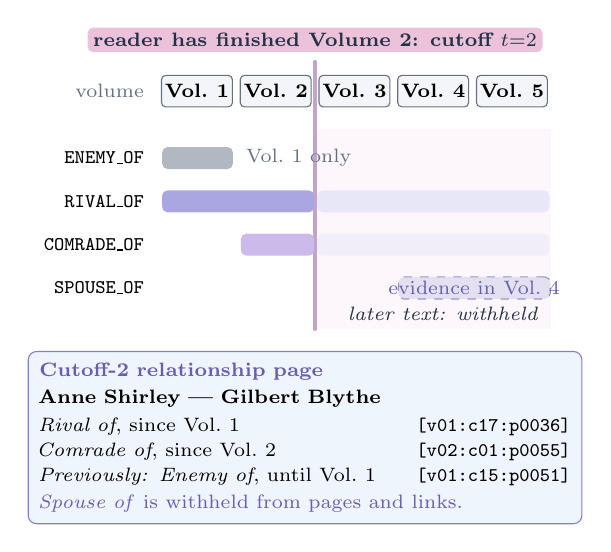
\begin{tikzpicture}[x=1.0cm, y=0.5cm, font=\scriptsize,
  vol/.style={draw=nwgray, fill=nwgraybg, rounded corners=1.5pt, minimum width=0.9cm, minimum height=0.4cm, inner sep=0pt},
  bar/.style={rounded corners=2pt, minimum height=0.28cm, inner sep=0pt, anchor=west},
  lab/.style={anchor=east, font=\figfont\ttfamily},
]
% volumes
\foreach \i in {1,...,5}{ \node[vol] (v\i) at (\i,0) {\textbf{Vol.~\i}}; }
\node[anchor=east, font=\figfont, text=nwgray, align=right] at (0.45,0) {volume};
% reader cutoff
\fill[nwredbg, opacity=0.6] (2.5,-0.95) rectangle (5.5,-6.05);
\draw[nwred!70!nwaccent, very thick, line cap=round] (2.5,0.75) -- (2.5,-6.05);
\node[fill=nwred, text=nwink, rounded corners=2pt, font=\figfont\bfseries, inner sep=2pt] at (2.5,1.3) {reader has finished Volume 2: cutoff $t{=}2$};
\node[text=nwink, font=\figfont\itshape, anchor=east] at (5.45,-5.65) {later text: withheld};
% intervals (stored first volume .. end)
\node[lab] at (0.45,-1.7) {ENEMY\_OF};
\node[bar, fill=nwgray!50, minimum width=0.9cm] at (0.55,-1.7) {};
\node[font=\figfont, text=nwgray, anchor=west] at (1.5,-1.7) {Vol.~1 only};
\node[lab] at (0.45,-2.8) {RIVAL\_OF};
\node[bar, fill=nwblue!75, minimum width=1.93cm] at (0.55,-2.8) {};
\node[bar, fill=nwblue!20, minimum width=2.95cm] at (2.52,-2.8) {};
\node[lab] at (0.45,-3.9) {COMRADE\_OF};
\node[bar, fill=nwgreen!75, minimum width=0.93cm] at (1.55,-3.9) {};
\node[bar, fill=nwgreen!20, minimum width=2.95cm] at (2.52,-3.9) {};
\node[lab] at (0.45,-5.0) {SPOUSE\_OF};
\node[bar, fill=nworange!28, draw=nworange, dashed, minimum width=1.93cm] at (3.55,-5.0) {};
\node[font=\figfont, text=nwaccent] at (4.52,-5.0) {evidence in Vol.~4};
% rendered page at t=2
\node[draw=nwblue!75!nwaccent, fill=nwbluebg, rounded corners=3pt, anchor=north west, text width=6.75cm, align=left, inner sep=4pt, font=\figfont]
  (page) at (-1.15,-6.6) {%
  {\scriptsize\bfseries\color{nwaccent}Cutoff-2 relationship page}\\[2pt]
  \textbf{Anne Shirley --- Gilbert Blythe}\\[2pt]
  \emph{Rival of}, since Vol.~1 \hfill{\ttfamily [v01:c17:p0036]}\\[1pt]
  \emph{Comrade of}, since Vol.~2 \hfill{\ttfamily [v02:c01:p0055]}\\[1pt]
  \emph{Previously: Enemy of}, until Vol.~1 \hfill{\ttfamily [v01:c15:p0051]}\\[2pt]
  {\color{nwaccent}\emph{Spouse of} is withheld from pages and links.}};
\end{tikzpicture}

\caption{Reading cutoffs for one character pair. Relation intervals open at their
first-evidence volume. The cutoff-2 wiki renders intervals opened by volume~2 and withholds
the marriage evidenced in volume~4. Citations use \texttt{v<volume>:c<chapter>:p<paragraph>}.}
\label{fig:cutoff}
\end{figure}
\fi
\paragraph{The relationship.} The relationship block (Figure~\ref{fig:qual-rel}) contains
the intervals illustrated in Figure~\ref{fig:cutoff}. At cutoff 2 it lists rivalry, the enmity that ended
in volume~1, comradeship and friendship, and its short prose ends with the two as close
friends. At cutoff 4 the same block adds ``Spouse of --- husband and wife (since v4)'', the
other lines cite more paragraphs, and the prose, written from the cutoff-4 claims only, ends
with the marriage. Each block's prose was generated independently from its cutoff's
filtered claim set.

\paragraph{Visible failure modes.} The example contains four defects. (i) The line
``Romantically involved with --- harbors romantic feelings
for her'' is open from volume~1 at both cutoffs. Its relation label is stronger than its
qualifier and evidence, producing \sys's uncertain disclosure verdicts
(Section~\ref{sec:results-main}). (ii) The cutoff-4 prose prints the keys by which the
generator names the lines it rests on (``[R3, R4, S1, S4]''). The renderer resolves those
keys into the \emph{Sources} line but fails to remove them from the prose; this occurs
on 5 of the 341 non-timeline pages at cutoff 4. (iii) The age ``nearly fourteen'', stated in volume~1, still
stands at cutoff 4 because an attribute with no later extracted value remains open. (iv) Gilbert's page
carries a second block, ``Shirley'' (Figure~\ref{fig:qual-rel}c). The reported build merged
the two entities the first build kept for ``Anne'' and ``Anne Shirley'', so the marriage is
now on Anne Shirley's block and on her page; a third entity under her surname remains, and
holds a rivalry line belonging to her. The screenshot shows the duplicate-entity failure
discussed in Appendix~\ref{app:additional}.

\newcommand{\qualshot}[2]{%
  \begin{minipage}{#1}%
  \begin{tcolorbox}[enhanced, width=#1, colback=white, colframe=nwlavender,
    boxrule=0.65pt, arc=3mm, outer arc=3mm,
    left=0pt, right=0pt, top=0pt, bottom=0pt, boxsep=0pt,
    before skip=0pt, after skip=0pt, clip upper]
    \includegraphics[width=\linewidth]{figures/qual/#2}%
  \end{tcolorbox}%
  \end{minipage}}

\begin{figure*}[p]
\centering
\begin{minipage}[t]{0.62\textwidth}\centering
\qualshot{\linewidth}{home.png}\\[2pt]
{\small (a) Home page: the reader picks a cutoff before seeing anything.}
\end{minipage}\\[10pt]
\begin{minipage}[t]{0.485\textwidth}\centering
{\small\bfseries Cutoff 2}\\[2pt]
\qualshot{\linewidth}{gilbert-v02-overview.png}\\[2pt]
{\small (b) Gilbert Blythe, overview, cutoff 2.}
\end{minipage}\hfill
\begin{minipage}[t]{0.485\textwidth}\centering
{\small\bfseries Cutoff 4}\\[2pt]
\qualshot{\linewidth}{gilbert-v04-overview.png}\\[2pt]
{\small (c) The same section, cutoff 4.}
\end{minipage}
\caption{The delivered site at two cutoffs (screenshots of the \sys wiki, Anne series).
Fields carry paragraph citations; at cutoff 4 the role, title and family lines
open intervals evidenced in volumes~3 and~4 and keep the earlier roles as closed intervals.}
\label{fig:qual-overview}
\end{figure*}

\begin{figure*}[p]
\centering
\begin{minipage}[t]{0.485\textwidth}\centering
{\small\bfseries Cutoff 2}\\[2pt]
\qualshot{\linewidth}{gilbert-v02-rel.png}\\[2pt]
{\small (a) Gilbert Blythe, relationship with Anne Shirley, cutoff 2.}
\end{minipage}\hfill
\begin{minipage}[t]{0.485\textwidth}\centering
{\small\bfseries Cutoff 4}\\[2pt]
\qualshot{\linewidth}{gilbert-v04-rel.png}\\[2pt]
{\small (b) The same block, cutoff 4: ``Spouse of'' opens in volume~4.}
\end{minipage}\\[10pt]
\begin{minipage}[t]{0.485\textwidth}\centering
\qualshot{\linewidth}{gilbert-v04-shirley.png}\\[2pt]
{\small (c) The block ``Shirley'' on the same page at cutoff 4: a second entity for Anne,
under her surname, holding one of her relations.}
\end{minipage}
\caption{One relationship at two cutoffs. Each block's prose is generated from its cutoff's
eligible claims; the cutoff-2 text therefore contains no marriage statement. The
bracketed keys in (b) and the block in (c) are defects of the reported build.}
\label{fig:qual-rel}
\end{figure*}

\paragraph{The same page as a structured comparison.} Table~\ref{tab:qual-diff} transcribes the
fields of Figures~\ref{fig:qual-overview} and~\ref{fig:qual-rel} side by side, separating the
intended interval behaviour from the four defects.

\begin{table*}[t]
\centering\footnotesize
\setlength{\tabcolsep}{4pt}
\renewcommand{\arraystretch}{1.15}
\begin{tabular}{@{}>{\raggedright\arraybackslash}p{2.35cm}>{\raggedright\arraybackslash}p{3.85cm}>{\raggedright\arraybackslash}p{4.45cm}>{\raggedright\arraybackslash}p{4.45cm}@{}}
\toprule
\nwhead{Field} & \nwhead{Cutoff 2 (\emph{Anne of Avonlea})} & \nwhead{Cutoff 4 (\emph{Anne's House of Dreams})} & \nwhead{Mechanism} \\
\midrule
\multicolumn{4}{@{}l}{\cellcolor{nwhighcyan}\nwhead{Intended behaviour}} \\
Role & teacher [v1 ch.\,XXXVI P24, v2 ch.\,I P55, +7] & country doctor (since v4) [v4 ch.\,14 P8]; \emph{previously:} teacher (v1--v2); Daily News employee (v3) & Supersession: an earlier value becomes a closed interval when a later one opens. \\
Titles & president (since v2) [v2 ch.\,VI P8] & adds Captain of the Freshman football team (v3), president of the Freshman Class (v3), doctor (v4) & Accumulation: volume-dated titles are appended; none is evicted. \\
Family & (no line) & Anne Shirley (spouse) & Withholding: no family claim has evidence by volume~2. \\
Anne--Gilbert block & rival; romantically involved with; saved; enemy (ended v1); comrade (since v2); friend (since v2) & the same six lines, with more citations, and \emph{Spouse of} --- husband and wife (since v4) [v4 ch.\,1 P5, ch.\,2 P7, ch.\,3 P29, +26] & History is kept as intervals; long context prints one line (``Spouse of --- husband, former schoolmate and college rival''). \\
Block prose & ends with the two as close friends & ends with the marriage & Each cutoff's prose is generated from its own filtered claims. \\
\midrule
\multicolumn{4}{@{}l}{\cellcolor{nwhighpink}\nwhead{Defects of the reported build}} \\
(i) Relation label & \emph{Romantically involved with} --- harbors romantic feelings for her, open from v1 [v1 ch.\,XXV P55] & unchanged & The label is stronger than its qualifier and evidence: \sys's uncertain disclosure verdicts (Section~\ref{sec:results-main}). \\
(ii) Line keys in prose & none & prose prints ``[R3, R4, S1, S4]'' and ``[R2, R7, S41, S67]'' & The renderer resolves keys into the \emph{Sources} line but leaves them in the prose: 5 of 341 non-timeline pages at $t{=}4$. \\
(iii) Age & nearly fourteen [v1 ch.\,XV P24] & nearly fourteen, beside the marriage & An attribute with no later extracted value stays open; elapsed years are not inferred. \\
(iv) Second entity & --- & a block ``Shirley'' holds \emph{Rival of} [v1 ch.\,XVII P36] & The build merged two of three Anne entities; the bare surname remains separate (Appendix~\ref{app:additional}). \\
\bottomrule
\end{tabular}
\caption{Gilbert Blythe's page in the reported \sys site at cutoffs~2 and~4, transcribed from
the delivered pages (screenshots are released with the code). Citations are printed as the
site prints them (volume, chapter, paragraph; ``+$n$'': further citations). Cyan: intended
interval behaviour; magenta: defects.}
\label{tab:qual-diff}
\end{table*}


\ifnwdecon% Appendix I: contamination diagnostics and the decontaminated condition (plan 0013 §4.3).
% Method from the implemented code; results from the ledger rows of 2026-10-03 to 2026-10-07 (all seven
% systems rebuilt at five cutoffs). Keys: results.tex, _build/fill_decon.py; DECON-* typed from the ledger.
\ifdefined\nwvtwo
\section{Contamination Diagnostics and the Treated Text}
\else
\section{Contamination Diagnostics and the Decontaminated Condition}
\fi
\label{app:contamination}

A generator may recognize published novels \citep{chang2023speak}. We compare aligned
original, names-only and renamed-and-paraphrased text, assessing recognition separately
from later-fact disclosure and cutoff compliance. Renaming follows prior practice
\citep{gupta2025whodunit, zhang2024infinitebench}; cross-condition differences motivate
contamination diagnostics \citep{dekoninck2024constat}. Because a treatment can damage
the narrative \citep{sun2025emperor}, we examine gold-fact fidelity and document errors.
The procedure aims to preserve facts, attribution, reveal order and cross-volume
coreference, but has no independent validation of complete fidelity. Reduced recognition
does not rule out memorization \citep{cheng2025contamination}.


\begin{figure}[t]
\centering
% F5 (one column, v2): gold recall of each system on the original and on the treated text,
% means over t=1..5. Dot positions are typed from the results.tex keys M1-anne-avg-<S> and
% M1-annedecon-avg-<S>; re-type them if those keys change. The printed changes are \res keys.
\begin{tikzpicture}[x=4.3cm, y=0.36cm, font=\figfont,
  orig/.style={circle, draw=nwgray, fill=white, line width=0.5pt, minimum size=5.2pt, inner sep=0pt},
  treat/.style={circle, fill=nwaccent, minimum size=3.2pt, inner sep=0pt},
  sysn/.style={anchor=west, font=\figfont\bfseries},
  dif/.style={anchor=east, font=\figfont, text=nwink}]
\foreach \x/\l in {0/0, 0.25/.25, 0.5/.50, 0.75/.75, 1/1}{
  \draw[nwgrid] (\x,0.55) -- (\x,-6.65);
  \node[text=nwgray] at (\x,-7.2) {\l};}
\node[anchor=west, font=\figfont\itshape, text=nwgray] at (-0.5,1.05) {system};
\node[font=\figfont\itshape, text=nwgray] at (0.5,1.05) {gold recall};
\node[anchor=east, font=\figfont\itshape, text=nwgray] at (1.24,1.05) {change};
% rows: name / y / original / treated / change
\newcommand{\dumb}[5]{%
  \node[sysn] at (-0.5,#2) {#1};
  \draw[nwgray, line width=0.7pt] (#3,#2) -- (#4,#2);
  \node[orig] at (#3,#2) {}; \node[treat] at (#4,#2) {};
  \node[dif] at (1.24,#2) {#5};}
\dumb{B1 long context}{0}{0.848}{0.845}{\res{M1-annedecon-diff-B1}}
\dumb{B2 prefix retrieval}{-1}{0.834}{0.784}{\res{M1-annedecon-diff-B2}}
\dumb{B3 LightRAG}{-2}{0.536}{0.470}{\res{M1-annedecon-diff-B3}}
\dumb{\sys}{-3}{0.802}{0.843}{\res{M1-annedecon-diff-B5}}
\dumb{B4 graph baseline}{-4}{0.761}{0.704}{\res{M1-annedecon-diff-B4}}
\draw[nwgrid, densely dotted] (-0.5,-4.55) -- (1.24,-4.55);
\dumb{X2 full text}{-5.1}{0.814}{0.744}{\res{M1-annedecon-diff-X2}}
\dumb{X1 closed book}{-6.1}{0.683}{0.003}{\best{\res{M1-annedecon-diff-X1}}}
% legend
\node[orig] at (-0.47,-8.25) {}; \node[anchor=west] at (-0.44,-8.25) {original text};
\node[treat] at (0.2,-8.25) {}; \node[anchor=west] at (0.23,-8.25) {treated (renamed, paraphrased)};
\end{tikzpicture}

\caption{Gold recall on original and treated text (means over $t=1..5$) and the change,
treated minus original. Without source text, recall collapses; with it, recall is largely
retained.}
\label{fig:deconrecall}
\end{figure}

\paragraph{Treatment.}
The treatment operates paragraph by paragraph, retaining identifiers, chapter boundaries
and scene breaks so citations remain aligned.

\emph{Step 1, names.} A reviewed map of \res{DECON-map} entries replaces character,
family and local place names with invented forms. Longer forms precede shorter ones
in whole-word replacement, with consistent full names, surnames and nicknames.
Mechanical checks require stand-ins to be absent from the source names and every part
of a mapped full name to be mapped. An initial map failed both checks after one volume:
a main character's stand-in matched two minor characters' first names, and a mapped
full name left its 148 bare-first-name occurrences unchanged. We rebuilt the map and
discarded that treated volume. Recurring minor characters and local places are renamed;
countries and distant cities remain. A surname also used as a compass direction is
replaced only in person-name contexts.

\emph{Step 2, paraphrase.} The generator rewrites each renamed paragraph under
instructions to preserve facts, events, numbers, places, ordering, names and dialogue
speakers, with no additions or summarization. Reapplying the map replaces any restored
source names. Nonempty rewrites between half and twice the source length are accepted;
otherwise the renamed paragraph is retained and counted as unparaphrased.
Residual source names are counted separately. In an initial treated volume,
approximately one paragraph in 25, containing one word in 12, retained at least four
fifths of its four-word sequences. We therefore request one retry when at least half
the source's four-word sequences remain. A second near-copy is retained but counted
as verbatim. Failed model calls stop the run, preventing silent fallback.

\emph{Step 3, gold.} The same map transforms the original gold facts and cast;
facts are neither added nor removed, and reveal volumes are unchanged.
All systems in Section~\ref{sec:setup} are rebuilt with unchanged code, configuration
and prompts. A names-only variant omits Step~2 and is used for recognition probes,
rather than complete system rebuilding.

\paragraph{What the condition can and cannot show.}
If systems mainly use supplied evidence, much of their original-text coverage may survive
the treatment. Reduced recognition may instead reduce closed-book coverage, where no
source text is supplied. These are diagnostic expectations, not an identification
strategy for each system's memory contribution: rewriting also changes wording,
entity resolution and sometimes meaning.

A prefix-bounded system can disclose later facts through extraction or inference errors,
generation or residual recognition. A treated-text disclosure by the full-text diagnostic
still demonstrates a failure to obey the cutoff while later evidence is available.
A model can recognize a plot without its original names, so the treatment cannot establish
the absence of memorization.

\paragraph{The treated text.}
The treated series contains \res{DECON-paras} paragraphs and
\res{DECON-words} words before and after treatment. Of these paragraphs,
\res{DECON-paraphrased} were paraphrased, with the remainder renamed only;
\res{DECON-verbatim} remained near-copies after retrying. Paraphrase lengthens the series
overall, although each accepted rewrite stays within the length bounds of Step~2.
Whole-name checks find no
mapped source name unchanged. A broader search finds
\res{DECON-residual-forms-n} inflected or derived source-name occurrences in
\res{DECON-residual-forms} paragraphs: chiefly family-name plurals (``the Gardners''),
plus a college-derived adjective and a sentence explaining a name's origin.
Recognition probes include these residual forms.

Some residuals reach generated pages. Across \res{DECON-pages-scanned} character pages
from seven systems, the name explained in the source sentence appears in
\res{DECON-jamesina-pages} pages of six systems. A family name retained in a plural
and a chapter title (``The Gardners' Call'') appears on
\res{DECON-gardner-pages} pages of four systems. Three other family names and the
college name, each from a residual form, appear on seven pages. A further
closed-book match is a common surname in an invented story.

Another source name has no literal residual: \res{DECON-pei-pages} pages from prefix
retrieval and the full-text diagnostic print ``Prince Edward Island'', absent from
the treated paragraphs and chapter titles. The renamed island's neighboring provinces
remain, permitting geographic inference. This output therefore does not distinguish
inference from residual recognition.

\paragraph{Fidelity.}
An unblinded LLM annotator checked all 111 gold facts against their treated evidence
paragraphs. It judged \res{DECON-fidelity} still expressed, one with altered wording:
a sleeve style is renamed in its evidence paragraph but given its source name in
the next paragraph. This asks whether the treated passage retains the fact.
The stricter paragraph-alone audit from Appendix~\ref{app:annotation}, yielding
\res{HUMR-gold} for the original text, was not repeated.

Errors also occur outside gold evidence. One paraphrase changes two children's ages
into an interval of minutes, after which prefix retrieval reports twins born six
minutes apart. The statement counts as supported against the supplied treated text.
Treatment errors found during analysis are documented here and left in place.

\paragraph{Recognition.}
On 200 aligned paragraphs spanning five volumes, the generator restores a masked
character name with accuracy \res{MEM-cloze-orig} on original text and
\res{MEM-cloze-decon} on treated text. Title identification is
\res{MEM-title-orig}, \res{MEM-title-remap} and \res{MEM-title-decon}
for original, names-only and combined treatment, respectively; author identification
is \res{MEM-author-orig}, \res{MEM-author-remap} and \res{MEM-author-decon}.
Renaming reduces title recognition more than author recognition. Adding paraphrase
reduces both further, to approximately one third of their names-only levels, but
roughly one treated paragraph in nine is still identified as belonging to the series.
Only recognition was probed for names-only text; complete systems were rebuilt on
original and combined-treatment text.

% The renamed-only control was probed for recognition; it is not an additional
% complete condition of the wiki comparison.
\begin{table}[t]
\centering\small
\setlength{\tabcolsep}{5pt}
\renewcommand{\arraystretch}{1.12}
\begin{tabular}{@{}lrr@{}}
\toprule
\nwhead{Text condition} & \nwhead{Title} & \nwhead{Author} \\
\midrule
Original & \res{MEM-title-orig} & \res{MEM-author-orig} \\
Names remapped & \res{MEM-title-remap} & \res{MEM-author-remap} \\
Remapped and paraphrased & \cellcolor{nwhighcyan}\res{MEM-title-decon} & \cellcolor{nwhighcyan}\res{MEM-author-decon} \\
\bottomrule
\end{tabular}
\caption{Recognition ablation on 200 aligned paragraphs. Values are the share for which
the frozen generator identifies an Anne title or its author. Renaming and paraphrasing
both reduce recognition, while residual recognition remains. Cyan highlights the combined
treatment. This probe does not establish
that a wiki fact was memorized.}
\label{tab:recognition}
\end{table}


\paragraph{Systems on the treated text.}
Table~\ref{tab:decon} compares original and treated systems;
Table~\ref{tab:decon-cells} reports every cutoff. Gold facts, reveal volumes and
labeling rules are transferred from the original; inverse name mapping allows
the same per-fact tests. Claude Opus~5.5 finalized the AI labels for all systems on both
texts, including precision and citation sufficiency.

Each condition has one build. Differences in entity resolution and paraphrase fidelity
preclude interpreting small cross-condition changes as isolated memory effects.
The closed-book diagnostic has a much larger recall reduction, from
\respt{M1-anne-avg-X1} to \respt{M1-annedecon-avg-X1}, with
\res{M1-annedecon-count-X1} matching fact--cutoff assessments remaining:
a death also present in its invented story. This is consistent with recognition
contributing substantially to original-text closed-book recall.

\paragraph{What the closed-book generator writes.}
Given stand-in names without text, the generator still writes full pages.
Of 200 sampled assertions, \res{M3-annedecon-unsup-X1} are unsupported.
The stand-in for a shy book-one farmer becomes a sea captain founding a cult;
a heroine's friend becomes a duelist at a magical academy; later cutoffs introduce
a street gang and a starship. Supported judgments concern generic statements
about gender, status, siblings or traits. No assertion carries a citation.

\paragraph{The disclosure by \sys.}
At $t=2$ and $t=3$, \sys lists both leads as spouses, a book-four fact
(\res{M4-annedecon-total-B5}, counting the marriage for both characters at both cutoffs).
These are two reciprocal subject facts from one prediction-to-marriage failure mechanism,
rather than four independent errors (Table~\ref{tab:disclosure-units}).
Another \res{M4-annedecon-uncertain-B5} verdicts are uncertain, involving the
same courtship line as in the original. The marriage citations point to a
book-two neighbor's prediction. Extraction stored a presumed marriage at
volume two, and rendering turned presumed spouses into spouses.
B4, using the same graph, prints ``anticipated future marriage'' at $t=2$,
labeled implied disclosure (\res{M4-annedecon-total-B4}).

The original build did not extract this relation from the corresponding passage.
The treated passage is cutoff-eligible, but the claim loses the distinction
between a character's prediction and an established event. Volume filtering
cannot repair that attribution and modality error.

\paragraph{Long-context prompting on the treated text.}
Mean recall is \respt{M1-annedecon-avg-B1} on treated text versus
\respt{M1-anne-avg-B1} on original text; precision is
\respt{M3-annedecon-avg-B1} versus \respt{M3-anne-avg-B1}.
Both treated estimates are lowest at $t=4$ (Table~\ref{tab:decon-cells}).
The close means do not establish equivalence from single builds.

Citation sufficiency is \respt{M8-annedecon-t1-B1} and
\respt{M8-annedecon-t2-B1} for one and two volumes, then falls to
\respt{M8-annedecon-t3-B1}, \respt{M8-annedecon-t4-B1} and
\respt{M8-annedecon-t5-B1}, versus \respt{M8-anne-t3-B1},
\respt{M8-anne-t4-B1} and \respt{M8-anne-t5-B1} on the original.
Most insufficient citations accompany supported assertions. Many retain the
paragraph number but lose the volume or chapter, pointing, for example, from
a volume-one fact to the corresponding identifier in volume three.
Such identifiers pass the harness's existence check.

The cause is untested. Familiarity with the original might help locate evidence,
or paraphrased passages might be harder to distinguish. Neither explanation
is isolated by this comparison.

\paragraph{The full-text diagnostic on the treated text.}
Despite the cutoff instruction, X2 discloses \res{M4-annedecon-total-X2}
assessed later facts on treated text, versus \res{M4-anne-total-X2} on the original.
Per-cutoff counts at $t=1..4$ are \res{M4-annedecon-t1-X2},
\res{M4-annedecon-t2-X2}, \res{M4-annedecon-t3-X2} and
\res{M4-annedecon-t4-X2}; original counts are \res{M4-anne-t1-X2},
\res{M4-anne-t2-X2}, \res{M4-anne-t3-X2} and \res{M4-anne-t4-X2}.
At $t=1$, the guardian's page describes the neighbor's widowhood and move,
the heroine's college attendance and her marriage ``years later''.
It cites volumes two to four, whose identifiers the harness accepts because
all volumes are supplied. Reduced recognition therefore does not make the
instruction reliable; observed disclosure is higher at the first cutoff.
Familiarity with the original's book boundaries is one untested explanation.

Treated recall is lower at every cutoff (\respt{M1-annedecon-avg-X2} versus
\respt{M1-anne-avg-X2}); mean precision is also lower
(\respt{M3-annedecon-avg-X2} versus \respt{M3-anne-avg-X2}).
Most unsupported statements are misattributed biographies, and citation errors
also omit volumes. The heroine's $t=1$ page returned malformed JSON three times,
closing a list with the wrong bracket. We corrected that bracket in the
recorded first response without another model call
(Appendix~\ref{app:reproducibility}).

\paragraph{Namesakes made by the name map.}
Whole-word renaming creates two collisions observed in the systems receiving the most
text, B1 and X2. First, one stand-in replaces a shared first name across characters,
making a book-one minor character a namesake of a schoolmate; passages about one
are then cited for the other. Second, a book-two twin's stand-in is a short form
of the stand-in for the heroine's romantic name, also borne by her friend's
daughter in book four. With book four in context, the twin's page describes
the friend (B1 at $t=4$; X2 at $t=2$, $4$ and $5$) or the heroine
(X2 at $t=3$), whereas original-text builds describe the twin.

This page contributes unsupported assertions and two stated X2 disclosures
at $t=3$. Neither mechanical map check detects these collisions. They are
treatment defects retained in the reported system scores.
\fi
% Appendix: observations made while building the systems that bear on the reported results.
\section{Development Observations}
\label{app:observations}

% The stored prompts are from a commercial development series: no value from it is printed (README, "Rules
% that are easy to break"; Ethical Considerations). The OBS-bake-* keys stay declared and unused.
\paragraph{Choice of generator.} We sent stored claim-extraction prompts from a commercial
development series to three Gemini Flash models, then checked the outputs of two of them,
3.1 Flash-Lite and 3.6 Flash, against their cited paragraphs. No numerical results from that series are reported
(Appendix~\ref{app:corpus}). Qualitatively, Gemini~3.1 Flash-Lite returned more facts than
Gemini~3.6 Flash, with a lower share fully supported and some unsupported claims; no
unsupported claims were observed in the reviewed 3.6 Flash outputs. We selected 3.6 Flash
for all stages and comparison systems. Model choice also affects entity discovery: from
the same volume-one Anne candidate list, Flash-Lite retained \res{OBS-gaz-lite} entities
and 3.6 Flash retained \res{OBS-gaz-f36}. This illustrates an effect on the entity inventory
before page generation.

\paragraph{Stories within the story.} Characters tell stories, invent companions and make
false confessions. Entity discovery admitted figures from embedded stories, including a
story-club heroine and a child's imagined cave lady, and verification accepted claims about
them (Appendix~\ref{app:evaluator}). Local evidence can therefore be insufficient to
distinguish the main narrative from an embedded or imagined account.

\paragraph{Reveal volumes need an earliest-statement check.} Disclosure assessment found
\res{OBS-gold-late} draft facts assigned reveal volumes later than their earliest supporting
statements. Pages containing these facts were consequently eligible. Reveal-volume
annotation requires searching for the earliest support, rather than retaining the first
passage encountered by the annotator.

\paragraph{Implicit temporal progression.}
Gilbert's age, \emph{nearly fourteen}, is extracted from volume one and remains on his
cutoff-4 page alongside the later marriage (Table~\ref{tab:qual-diff}). No extracted
age supersedes it, so its interval stays open. The graph records explicit changes; it does
not advance ages with narrative time. Reveal volumes order evidence rather than elapsed
story years. A historical age should therefore be marked as an observation at a particular
story time unless a supported update is available.

\paragraph{Cross-claim inference.}
Some updates require combining claims rather than extracting one explicit statement.
As an illustrative example, suppose Anne is two years younger than Gilbert and marries
him at age 25. The premises imply that Gilbert is 27 at their marriage. These ages are
hypothetical, not verified annotations of the displayed example. The current pipeline
does not systematically derive such updates. An extension would need to retain the
supporting premises, align their narrative times and expose a derived claim only after
all required premises become available at the reader's cutoff.

\paragraph{Coreference across extraction windows.}
Pronouns and other referring expressions can link a character or fact across sentences
and scenes without repeating a name. Extraction may miss these links or attribute a
claim to the wrong person when the relevant context lies outside its window. Both backward
and forward references require discourse context, while a later identity revelation must
remain unavailable at an earlier cutoff. These are qualitative failure modes; no error
rate for them is measured here.

% Appendix: reproducibility and release.
\section{Reproducibility and Release}
\label{app:reproducibility}

\paragraph{Freeze.} Before each block of runs, the source code, configuration, and scripts
are hashed into a freeze record that every runner checks before making a call. Any change
requires a new record and an account of which results it invalidates. Changes affecting a
reported number are logged with the previous and revised values and the cells rebuilt or
relabeled, including the two label audits in Section~\ref{sec:setup}.
Sampling seeds are fixed (assertion samples: seed 0).

\paragraph{Provenance.} A shared client caches every model response under a hash of its
provider, model, prompt, and parameters; each run writes a manifest and call log. Every number
in the paper maps to a measurement-ledger row identifying the producing command and run.
All generative calls of the systems and of the treatment used \res{GEN-model}, between 28 September and
\ifnwdecon 7\else 5\fi{} October 2026. The provider's model name exposes no finer revision.
Cached responses reproduce the released artifacts exactly; fresh calls need not produce
identical generations.\ifnwdecon{} On the treated text, \res{DECON-recovered} page of the
full-text diagnostic returned a list with an incorrect closing bracket in three attempts.
The runner corrected the bracket in the recorded first response and applied its normal
validation and rendering; no page was regenerated.\fi{} Appendix~\ref{app:prompts} lists
every generative stage with its logged call and prints two exchanges in full; the release
holds one complete logged exchange per stage, with system prompt, input and output. Claude Opus~5.5 finalized all reported AI annotation labels after evidence review.
The prompt and response defects documented in Appendix~\ref{app:prompts} remain part of
the archived run configuration. The reported results are not measurements of a repaired
prompt builder or citation validator.

\paragraph{Commands.} With the corpus parsed, the reported artifacts are produced by:
\begin{itemize}[leftmargin=*,itemsep=1pt,topsep=2pt]
  \raggedright
  \item the reported \sys build of all five cutoffs:\\ \texttt{\small run\_series.py anne@v2 -{}-upto 5}
    (the first build is the series \texttt{\small anne});
  \item a comparison cell at cutoff $t$:\\ \texttt{\small run\_baseline.py anne \{X1|B1|B2|B4|X2\} -{}-upto t},
    with \texttt{\small -{}-chunk-words 150 -{}-budget-tokens 20000} for B2 and
    \texttt{\small -{}-graph anne@v2 -{}-budget-tokens 20000} for B4, and
    \texttt{\small b3\_lightrag.py anne -{}-upto t -{}-mode mix};
  \item the assertion inventory and sample of a cell:\\ \texttt{\small assertion\_inventory.py S -{}-upto t} and
    \texttt{\small assertion\_precision.py S -{}-upto t -{}-n 40 -{}-population all};
  \item disclosure candidates:\\ \texttt{\small m4\_tree.py S -{}-upto t};
  \item the lexical screen:\\ \texttt{\small artifact\_exposure.py S};
  \item the pair rule and the timeline citations applied to a cell's labels:\\ \texttt{\small apply\_pair\_rule.py S B5};
  \item table values:\\ \texttt{\small paper\_numbers.py}; their spread over cutoffs:\\ \texttt{\small summary\_stats.py};
  \item cost of the cells on disk:\\ \texttt{\small run\_cost.py S -{}-final}.
\end{itemize}

\paragraph{Release.} An anonymized archive provides the submission materials; the repository
address is \anonrepo. It contains the code, configuration, dependency specification and freeze records;
prompt templates and logged exchange excerpts; gold facts with evidence identifiers and reveal volumes;
and AI evaluation label files
(recall, annotated precision samples, citation sufficiency, disclosure verdicts with the
sentences assessed, and audit corrections). It also includes per-run cost summaries, every
system's generated wikis at every cutoff, both builds of \sys, and the human-review package
(\res{ANN-n-total} items with source context: every gold fact and samples of the recall,
precision and citation labels), plus the two reviewers' label files, accompanying records,
provenance manifest, aligned decision audit and recomputed agreement. The reviewer labels
are entirely human-produced. The source texts
are public-domain and are fetched from Project Gutenberg by identifier.

% Appendix O (v3): prompt and defect architecture. The v2 appendix printed every logged exchange in
% full (about 30 pages); v3 keeps one table of every exhibited stage, the two exchanges a reader
% needs to reproduce the method, and the documented defects as callouts. The complete exchanges
% are unchanged in docs/paper/appendix/k-prompts.tex (v1/v2) and in the released call logs;
% excerpts below are copied from them verbatim (scripts/papers/prompt_appendix.py).
\clearpage
\onecolumn
\begingroup
\newtcblisting{nwprompt}[3][]{
  enhanced, breakable, listing only,
  colback=#2!8!white, colframe=#2,
  colbacktitle=#2!35!white, coltitle=nwink,
  title={#3}, fonttitle=\sffamily\bfseries\footnotesize,
  boxrule=0.45pt, arc=1.5mm, left=1.5mm, right=1.5mm, top=1mm, bottom=1mm,
  before skip=5pt, after skip=6pt,
  listing options={basicstyle=\ttfamily\scriptsize, columns=fullflexible, keepspaces=true,
    breaklines=true, breakatwhitespace=false, breakindent=1em, showstringspaces=false,
    frame=none, aboveskip=0pt, belowskip=0pt},
  #1}
\newtcolorbox{nwdefect}[1]{enhanced, breakable, colback=nwhighpink!45!white, colframe=nwMagenta,
  boxrule=0.5pt, arc=1.5mm, left=2mm, right=2mm, top=1mm, bottom=1mm, before skip=6pt,
  after skip=6pt, title={#1}, fonttitle=\sffamily\bfseries\footnotesize, colbacktitle=nwmagenta,
  coltitle=nwink, fontupper=\small}

\section{Prompts and Model Exchanges}
\label{app:prompts}
Every generative stage calls the generator through one client that records the system prompt,
the user prompt and the raw response. Table~\ref{tab:prompt-stages} lists the stages whose
first successful call from the run behind the reported results is exhibited in the release;
all used \res{GEN-model}. It first prints the two exchanges a reader needs to reproduce the method (same-volume
arbitration and the paraphrase that makes the treated text) and the five defects that the
logged prompts and responses carry; the complete logged exchange of every stage follows
(Appendix~\ref{app:prompts-full}). Every call log is released
(Appendix~\ref{app:reproducibility}); the excerpts are verbatim, with elisions marked. Evaluation labels were not produced by
these stages (Appendix~\ref{app:annotation}).

\begin{table*}[t]
\centering\footnotesize
\setlength{\tabcolsep}{4pt}
\begin{tabular}{@{}>{\raggedright\arraybackslash}p{3.0cm}>{\raggedright\arraybackslash}p{6.3cm}r>{\raggedright\arraybackslash}p{3.75cm}@{}}
\toprule
\nwhead{Stage} & \nwhead{Role} & \nwhead{Tokens in / out} & \nwhead{Run} \\
\midrule
\multicolumn{4}{@{}l}{\emph{\sys build}} \\
Entity typing & Types each mined name candidate (gazetteer) (\emph{``Anne'', v1}) & 518 / 39 & \nolinkurl{20261004T193719-gazetteer-v1-5} \\
Alias adjudication & Decides whether two surface forms are one entity (gazetteer) (\emph{Charlie vs.\ Carrie Sloane}) & 548 / 50 & \nolinkurl{20261004T193719-gazetteer-v1-5} \\
Claim extraction & Extracts dated, quoted claims about one character from one evidence window (\emph{Anne Shirley, v5}) & 8,884 / 734 & \nolinkurl{20261005T070204-extract-v5-5} \\
Scene extraction & Records scenes, participants and events over a chapter span (\emph{v5, chapter 2}) & 5,729 / 202 & \nolinkurl{20261004T195945-scenes-v5-5} \\
Infobox pass & Long-context pass for gender, age and origin (\emph{Anne Shirley, v1}) & 93,403 / 490 & \nolinkurl{20261005T070216-infobox-v1-5} \\
Backstory pass & Long-context pass for background facts (\emph{Marilla Cuthbert, v1}) & 135,267 / 309 & \nolinkurl{20261005T070229-backstory-v1-5} \\
Arbitration & Resolves a same-volume conflict between two values (\emph{Anne Shirley, AGE, v1}) & 258 / 55 & \nolinkurl{20261005T070243-graph_build-v1-5} \\
Verification & Checks a stored fact against its own cited evidence (\emph{Anne Shirley, APPEARANCE}) & 2,833 / 5 & \nolinkurl{20261005T053635-verify-upto5} \\
\midrule
\multicolumn{4}{@{}l}{\emph{\sys publication}} \\
Page prose (appearance) & Writes a physical description from the cutoff-filtered claims (\emph{Anne Shirley, $t{=}1$}) & 1,045 / 174 & \nolinkurl{20261005T070347-synthesize-upto5} \\
Codex summary & Writes the one-sentence summary of a shared codex entry (\emph{Aid Society, $t{=}1$}) & 1,974 / 69 & \nolinkurl{20261005T070527-site_build-upto5} \\
\midrule
\multicolumn{4}{@{}l}{\emph{Comparison systems and diagnostics}} \\
B1 page & Long context: one character page from the whole prefix (\emph{Anne Shirley, $t{=}4$}) & 559,824 / 5,688 & \nolinkurl{20261001T043209-baseline-b1-v4} \\
B2 page & Prefix retrieval: one character page from retrieved passages (\emph{Marilla Cuthbert, $t{=}1$}) & 24,083 / 2,477 & \nolinkurl{20261002T095544-baseline-b2-v1} \\
B3 index & LightRAG's own entity and relation extraction while building its index & 3,243 / 1,022 & \nolinkurl{20260929T225346-baseline-b3-v5} \\
B3 page & LightRAG: one character page from LightRAG context (\emph{Anne Shirley, $t{=}5$}) & 17,438 / 2,191 & \nolinkurl{20261001T142328-baseline-b3-v5} \\
X1 page & Closed book: title and character name only (\emph{Matthew Cuthbert, $t{=}5$}) & 451 / 1,087 & \nolinkurl{20260930T214444-baseline-x1-v5} \\
X2 page & Full text: all five volumes and the cutoff instruction (\emph{Gilbert Blythe, $t{=}1$}) & 689,967 / 2,449 & \nolinkurl{20260930T222548-baseline-x2-v1} \\
\midrule
\multicolumn{4}{@{}l}{\emph{Treated text and recognition}} \\
Paraphrase & Paraphrases one renamed paragraph & 385 / 209 & \nolinkurl{20261003T165238-decontaminate-v5} \\
Memorization probe & Name cloze or title identification on one paragraph & 227 / 9 & \nolinkurl{20261003T165318-probe-memorization-v1-5} \\
\bottomrule
\end{tabular}
\caption{Every exhibited model stage: the first successful call of the run behind the reported
results, with the exhibited character or entry and volume or cutoff in italics. Runs are under \nolinkurl{anne@v2/} (build and pages) or \nolinkurl{anne-decon/}
(treatment and probe) in the release. B4's page prompt, the other prose sections and the
shared-page summary check are in the release only.}
\label{tab:prompt-stages}
\end{table*}

\subsection*{Same-volume arbitration}
Two values of one attribute from one volume are treated as an extraction conflict
(Section~\ref{sec:method}). A \texttt{flag} resolution keeps the higher-confidence value
provisionally (here 11), so the interval sequence has no gap, and records the conflict.
\begin{nwprompt}{nwViolet}{User prompt (system prompt in the release)}
Character: anne-shirley
Attribute: AGE
Volume: 1

Fact A: value="11", confidence=1.00, evidence: "I was eleven last March," said Anne"
Fact B: value="13", confidence=0.99, evidence: "It's such a solemn thing to be almost fourteen, Marilla."; ""Just think, Diana, I'm thirteen years old today," remarked Anne in an awed voice."

Which fact is correct? resolution must be one of keep_a, keep_b, keep_both, flag, plus a one-sentence rationale citing the evidence.
\end{nwprompt}
\begin{nwprompt}{nwCyan}{Model output}
{"resolution": "flag",
 "rationale": "Fact A states Anne was eleven based on an earlier passage, while Fact B shows her turning thirteen later in the same volume, indicating a progression of time rather than a single static age."}
\end{nwprompt}

\subsection*{Paraphrase for the treated text}
Each renamed paragraph is paraphrased in one call, keeping its identifier.
\begin{nwprompt}{nwViolet}{System and user prompt (paragraph abridged)}
SYSTEM: You rewrite passages of fiction in new words for a research corpus. You never add, remove or explain anything.

Rewrite the paragraph below in different words and different sentence structure.
Rules:
- Keep every fact, event, number, date and place, and keep them in the same order.
- Keep every personal and ship name exactly as written. Do not introduce any name that is not in the paragraph.
- Dialogue stays dialogue, spoken by the same person. Use the same quotation marks as the original (" " stay " "). Only spoken words go inside them; a speech tag such as "said I" stays outside.
- Keep the narrator's person (first person stays first person).
- Do not summarise, shorten substantially, or add commentary.
Return only the rewritten paragraph, nothing else.

Paragraph:
It was a clear, apple-green evening in May, and Seven Gulls Harbour was mirroring back the clouds of the golden west between its softly dark shores. [...]
\end{nwprompt}
\begin{nwprompt}{nwCyan}{Model output (abridged)}
The May evening was transparent and apple-green, as Seven Gulls Harbour reflected the clouds from the golden west amidst its gently darkened banks. [...]
\end{nwprompt}

\subsection*{Defects carried by the logged prompts and responses}
The five defects below are part of the reported runs. They are documented, not repaired;
Section~\ref{sec:discussion} and Appendix~\ref{app:formal} relate each to the results.

\begin{nwdefect}{D1\enspace Implementation notes used as field definitions (extraction and verification)}
The extraction prompt defines STATUS and APPEARANCE with internal revision labels and code
paths, and the verifier is told to judge an APPEARANCE fact by that same text:
\begin{nwprompt}{nwMagenta}{Verification user prompt (excerpt)}
Fact: APPEARANCE = "little pale face with seven freckles on the nose" -- evidence: [v02:c27:p0041] [...]
Definition of APPEARANCE: subsume (Phase 22 A2): drop a value that is redundant next to a longer sibling ('hair' next to 'long brown hair') or a bare single-word noun standing alone -- see graph/canonicalize.py::subsume_values. Deterministic, no embed call.
\end{nwprompt}
The exhibited claim is accepted; the example alone does not measure the defect's effect.
\end{nwdefect}

\begin{nwdefect}{D2\enspace Responses depart from prompt rules the code does not enforce (infobox pass)}
The volume-1 infobox response gives a \texttt{GENDER} quote that does not contain Anne's
name, and two \texttt{AGE} values (11 and 13). The code applies the evidence gates of
Section~\ref{sec:method}, not these two prompt rules; the two ages go to arbitration, shown
above.
\end{nwdefect}

\begin{nwdefect}{D3\enspace Early-volume prompts carry later aliases}
Alias lists come from the whole-series entity index, so the volume-1 infobox call already
names Anne by her married names:
\begin{nwprompt}{nwMagenta}{Infobox user prompt, volume 1 (excerpt)}
Character: "Anne Shirley" (aliases: Anne, Anne-girl, Mistress Blythe, Mrs. Blythe, Mrs. Doctor, Mrs. Doctor, dear, Mrs. Dr. dear, Queen Anne, the Anne-girl, young Mrs. Doctor)
Volume 1.
\end{nwprompt}
This is construction dependence reaching the generator's input
(Section~\ref{sec:results-scope}); the comparisons of this paper do not isolate it.
\end{nwdefect}

\begin{nwdefect}{D5\enspace A response cites a paragraph ID where a line key was requested (codex summary)}
The codex prompt asks the model to cite input-line keys such as \texttt{W1}; the response
returns \texttt{v01:c27:p0000}, a paragraph ID. The parser normalizes returned paragraph IDs
during citation resolution, which maps an identifier to a paragraph but does not check that
the paragraph supports the sentence.
\end{nwdefect}

\begin{nwdefect}{D4\enspace Residue of one prompt serving every corpus}
The typing prompt lists a type unused here (\texttt{TECH}) and, as logged, repeats one example
sentence three times; the extraction prompt's JSON example uses a character from another
series (``Shin''); the paraphrase rule keeps ``personal and ship'' names, which has no effect
on this series.
\end{nwdefect}
\endgroup

% Logged exchanges from scripts/papers/prompt_appendix.py; layout polished for submission.
% Preserve the content of every listing when regenerating this appendix.
% Two-column like every other appendix (ACL formatting guidelines); the listing boxes break
% across columns and pages.
\begingroup
\definecolor{NWPromptIndigo}{HTML}{C9C7EB}
\definecolor{NWPromptCyan}{HTML}{C8EAF5}
\definecolor{NWPromptViolet}{HTML}{DDCEEE}
\definecolor{NWPromptInk}{HTML}{243247}
\newtcblisting{nwprompt}[3][]{
  enhanced, breakable, listing only,
  colback=#2!12!white, colframe=#2!85!white,
  colbacktitle=#2, coltitle=NWPromptInk,
  title={#3}, title after break={#3 (continued)},
  fonttitle=\sffamily\bfseries\small,
  boxrule=0.45pt, arc=1.5mm,
  left=2mm, right=2mm, top=1.5mm, bottom=1.5mm,
  before skip=7pt, after skip=9pt,
  pad at break*=1.5mm,
  listing options={
    basicstyle=\ttfamily\footnotesize,
    columns=fullflexible, keepspaces=true,
    breaklines=true, breakatwhitespace=false, breakindent=1em,
    showstringspaces=false, showspaces=false, showtabs=false,
    frame=none, aboveskip=0pt, belowskip=0pt, tabsize=2
  },
  #1
}
\subsection{Complete logged exchanges}
\label{app:prompts-full}
Every generative stage uses a shared client that records the system prompt, user prompt, and raw response. For each stage, we show the first successful call from the latest run underlying the reported results that sent calls to the provider. The exhibits cover each \sys stage (prose by its appearance section), the B1, B2, B3, X1 and X2 pages, the treatment and the recognition probe; B4's page prompt, the other prose sections and the shared-page summary check are in the release only. The exchanges retain the logged wording, with middle elisions that state the number of omitted characters and typographic characters folded to ASCII for typesetting. All calls shown used \res{GEN-model}. The release contains the complete prompts and call logs (Appendix~\ref{app:reproducibility}). Evaluation labels were not produced by these stages; the annotation workflow is described in Appendix~\ref{app:annotation}.

The excerpts retain defects in the prompts and responses used for the reported runs.
The notes below identify these defects without rewriting the logged exchanges or claiming
that the pipeline has been repaired (Appendix~\ref{app:implementation}).

\Needspace{12\baselineskip}
\subsection*{Entity typing}
Types each mined name candidate (\sys, gazetteer). Model \texttt{gemini-3.6-flash}; 518 input and 39 output tokens; run \nolinkurl{anne@v2/20261004T193719-gazetteer-v1-5}.

\paragraph{Note on this log.} One prompt serves every series the pipeline processes, so the
type list includes types unused here (\texttt{TECH}). The example sentences are logged as
sent: one sentence appears three times.

\begin{nwprompt}{NWPromptIndigo}{System prompt}
You are typing candidate names mined from a novel. Each candidate is a capitalised phrase that occurs in the text; most are real entities but some are sentence fragments, honorific-only phrases, or common words that happened to be capitalised.

Classify the candidate into exactly one of these types, or say it is not an entity at all:
- CHARACTER
- FACTION
- LOCATION
- EVENT
- TECH

If the candidate is not a named entity -- a stray common word, part of a longer name cut short, a rank or honorific with no name attached -- respond with entity_type "NOT_ENTITY". This is a correct and expected answer for a large share of candidates; do not force a fit.

Respond with JSON only: {"entity_type": "...", "confidence": 0.0-1.0, "notes": "short reason"}
\end{nwprompt}

\begin{nwprompt}{NWPromptViolet}{User prompt (input)}
Candidate surface: "Anne"
Seen 3904 time(s), first in volume 1.
Mining signals: capitalised_token, honorific, vocative
Example sentences it appears in:
- ""Anne Shirley," reluctantly faltered forth the owner of that name, "but, oh, please do call me Cordelia. It can't matter much to you what you call me if I'm only going to be here a little while, can it? And Anne is such "
- ""Unromantic fiddlesticks!" said the unsympathetic Marilla. "Anne is a real good plain sensible name. You've no need to be ashamed of it.""
- ""Oh, I'm not ashamed of it," explained Anne, "only I like Cordelia better. I've always imagined that my name was Cordelia--at least, I always have of late years. When I was young I used to imagine it was Geraldine, but I "
- ""Oh, I'm not ashamed of it," explained Anne, "only I like Cordelia better. I've always imagined that my name was Cordelia--at least, I always have of late years. When I was young I used to imagine it was Geraldine, but I "
- ""Oh, I'm not ashamed of it," explained Anne, "only I like Cordelia better. I've always imagined that my name was Cordelia--at least, I always have of late years. When I was young I used to imagine it was Geraldine, but I "

What is this?
\end{nwprompt}

\begin{nwprompt}{NWPromptCyan}{Model output}
{"entity_type": "CHARACTER", "confidence": 1.0, "notes": "Anne (Anne Shirley) is the main character of the novel Anne of Green Gables."}
\end{nwprompt}

\Needspace{12\baselineskip}
\subsection*{Alias adjudication}
Decides whether two surface forms are one entity (\sys, gazetteer). Model \texttt{gemini-3.6-flash}; 548 input and 50 output tokens; run \nolinkurl{anne@v2/20261004T193719-gazetteer-v1-5}.

\begin{nwprompt}{NWPromptIndigo}{System prompt}
You are deciding whether two surface forms mined from a novel refer to the SAME entity (e.g. a full name and a nickname, a call sign and a real name, a title and a bare surname) or to two DIFFERENT entities that merely look similar.

Leaving two different surface forms unmerged is the SAFE error -- a human reviewer can merge them in five seconds. Merging two different people is the COSTLY error -- it silently mixes their facts on one page and is hard to catch later. When genuinely unsure, say they are different.

Decide from the quoted passages alone. Anything you may know about this book or its series from elsewhere is not evidence: the reader of this page knows only the text so far, and a merge the passages do not show can reveal a later twist or join two different people.

Respond with JSON only: {"same_entity": true/false, "confidence": 0.0-1.0, "notes": "short reason"}
\end{nwprompt}

\begin{nwprompt}{NWPromptViolet}{User prompt (input)}
Form A: "Charlie Sloane" (CHARACTER, seen 38 time(s), first vol 1):
  - "in half a dozen take-notices. "It's only meant as a joke. And don't you be too sure your name won't ever be written up. Charlie Sloane is dead gone on you. He told his mother--his mother, mind you--that you were the smartest girl in school. That's better than being good-looking.""
  - ""No, it isn't," said Anne, feminine to the core. "I'd rather be pretty than clever. And I hate Charlie Sloane, I can't bear a boy with goggle eyes. If anyone wrote my name up with his I'd never get over it, Diana Barry. But it is nice to keep head of your class.""

Form B: "Carrie Sloane" (CHARACTER, seen 10 time(s), first vol 1):
  - "der brothers and sisters who were going to take part. Everybody in school over nine years of age expected to go, except Carrie Sloane, whose father shared Marilla's opinions about small girls going out to night concerts. Carrie Sloane cried into her grammar all the afternoon and felt that life was n"
  - "a model pupil like Minnie Andrews. She hadn't anything on her conscience. The girls cried all the way home from school. Carrie Sloane kept saying every few minutes, 'The time has come for us to part,' and that would start us off again whenever we were in any danger of cheering up. I do feel dreadful"

Are these the same entity?
\end{nwprompt}

\begin{nwprompt}{NWPromptCyan}{Model output}
{"same_entity": false, "confidence": 1.0, "notes": "Charlie Sloane (a male classmate described as a boy) and Carrie Sloane (a female classmate) are two distinct individuals/siblings within the same family."}
\end{nwprompt}

\Needspace{12\baselineskip}
\subsection*{Claim extraction}
Extracts dated, quoted claims about one character from one evidence window (\sys). Model \texttt{gemini-3.6-flash}; 8,884 input and 734 output tokens; run \nolinkurl{anne@v2/20261005T070204-extract-v5-5}.

\paragraph{Note on this log.} STATUS and APPEARANCE include internal revision labels,
code paths, and implementation notes in the prompt's field descriptions. These entries
are preserved as run evidence. Implementation metadata should be separated from semantic
definitions in the prompt builder before future runs.

\begin{nwprompt}{NWPromptIndigo}{System prompt}
You are extracting facts about ONE named character from passages of a novel. You will be told the character's name; extract facts ONLY about that character, never about anyone else named alongside them.

Three kinds of fact exist:

ATTRIBUTE (a scalar fact about the character):
- AGE
- GENDER
- STATUS -- alive / deceased / missing in action / captured. Use polarity=presumed when the text only reports a belief. `default` (Phase 22 A5, U6): materialized by synth/assemble.py when zero STATUS claims exist -- 'alive' is the reader's safe default at any cutoff (a later death is itself a claim that only appears once the reader reaches it), marked inferred: true so it never masquerades as evidence.
- RANK -- A formal grade inside a named organisation or hierarchy: a military rank, a guild or adventurer grade, a noble or church rank. Always a category, never a number. NOT a power level, a game level or any other statistic, NOT a job (OCCUPATION), NOT an honorific or epithet (TITLE).
- TITLE -- An honorific, epithet or office the text calls the character by (Supreme Being, the Wisewolf of Yoitsu, head of the branch). A grade in a hierarchy is RANK; a job is OCCUPATION.
- NICKNAME -- Includes call signs and code names. first_vol matters: an alias revealed in V3 must not appear on a V1 page.
- ORIGIN -- Where the character comes from: a birthplace, homeland, village or people. Never a job or a past occupation (that is OCCUPATION or BACKGROUND).
- OCCUPATION -- What the character does in the world: their job, trade or standing role (merchant, maid, village chief, floor guardian). NOT a combat class or skill, NOT a species, NOT a rank.
- APPEARANCE -- subsume (Phase 22 A2): drop a value that is redundant next to a longer sibling ('hair' next to 'long brown hair') or a bare single-word noun standing alone -- see graph/canonicalize.py::subsume_values. Deterministic, no embed call.

RELATION (a link to another character or entity actually named in the passage; "object" must be copied verbatim from a name that appears in the passage, not paraphrased or described):
- PARENT_OF -- An actual stated parent/child relationship -- never inferred from a shared surname, a title like 'son of', or 
[... 9,813 characters elided ...]
BLING_OF, SPOUSE_OF, STUDENT_OF), not just the subject.

Respond with JSON only, shaped exactly like this worked example (a RELATION fact about a
character named "Shin", using null for the fields a TRAIT or ATTRIBUTE fact would instead need):

{"facts": [
  {"predicate": "AFFILIATED_WITH", "kind": "relation", "object": "Spearhead Squadron", "value": null, "qualifier": "captain", "para_id": "v01:c00:p0031", "quote": "the Spearhead Squadron's captain, code name Undertaker", "confidence": 0.92, "polarity": "asserted"}
]}

Return {"facts": []} if this passage says nothing new about this character.
\end{nwprompt}

\begin{nwprompt}{NWPromptViolet}{User prompt (input)}
Character: "Anne Shirley" (aliases: Anne, Anne-girl, Mistress Blythe, Mrs. Blythe, Mrs. Doctor, Mrs. Doctor, dear, Mrs. Dr. dear, Queen Anne, the Anne-girl, young Mrs. Doctor)
Volume 5.
Other people/things named in these passages: Aunt Martha (also: old Martha), Avonlea (also: The Avonlea), Blythe, Carl, Cornelia Bryant (also: Bryant, Cornelia, Cornelia Elliott, Miss Bryant, Miss Cornelia, Mrs. Elliott, Mrs. Marshall Elliott, fair Cornelia), Europe, Faith (also: Faith Meredith, Red Rose), Four Winds, Four Winds Harbor (also: Four Winds Harbour), Glen, Green Gables, Harbour Head, Harrison, Ingleside, James A (also: James), Jem (also: Jem Blythe, Little Jem), Jerry Corcoran (also: Jerry), London, Maria, Marilla Cuthbert (also: Aunt Marilla, Cuthbert, Marilla, Miss Cuthbert), Mary Vance (also: Mary, Mary-creature), Methodist (also: Methodists, The Methodists), Paul Irving (also: Paul), Presbyterian (also: Presbyterians), Priscilla Grant (also: Grant, Pris, Priscilla, Prissy, Prissy Andrews), Rachel Lynde (also: Lynde, Mrs. Rachel, Rachel), Rainbow Valley, Rilla Blythe (also: Rilla), Shirley, Susan (also: Susan Baker, old Susan, old Susan Baker), Taylor, Thomas Lynde (also: Rachel Lynde's husband, Thomas), Una Meredith (also: Una), Walter Blythe (also: Walter)

Passages (each paragraph labeled with its id; a passage break means the text on either side comes from a different part of the volume and does not continue):
[v05:c01:p0000] It was a clear, apple-green evening in May, and Four Winds Harbour was mirroring back the clouds of the golden west between its softly dark shores. The sea moaned eerily on the sand-bar, sorrowful even in spring, but a sly, jovial wind came piping down the red harbour road along which Miss Cornelia's comfortable, matronly figure was making its wa
[... 18,642 characters elided ...]
ained untinged of charity. Susan smiled slyly.
[v05:c02:p0042] "They do say, Mrs. Marshall Elliott, that the Methodists and Presbyterians are talking of uniting," she said.
[v05:c02:p0043] "Well, all I hope is that I'll be under the sod if that ever comes to pass," retorted Miss Cornelia. "I shall never have truck or trade with Methodists, and Mr. Meredith will find that he'd better steer clear of them, too. He is entirely too sociable with them, believe me. Why, he went to the Jacob Drews' silver-wedding supper and got into a nice scrape as a result."

Extract facts about "Anne Shirley" only.
\end{nwprompt}

\begin{nwprompt}{NWPromptCyan}{Model output}
{"facts": [
  {"predicate": "SPOUSE_OF", "kind": "relation", "object": "Blythe", "value": null, "qualifier": "husband", "para_id": "v05:c01:p0001", "quote": "Miss Cornelia was going up to Ingleside to see Dr. and Mrs. Blythe, who were just home from Europe.", "confidence": 0.95, "polarity": "asserted"},
  {"predicate": "PARENT_OF", "kind": "relation", "object": "Rilla Blythe", "value": null, "qualifier": "mother", "para_id": "v05:c01:p0003", "quote": "Behind her, in the hammock, Rilla Blythe was curled up, a fat, roly-poly little creature of six years, the youngest of the Ingleside children.", "confidence": 0.95, "polarity": "asserted"},
  {"predicate": "PARENT_OF", "kind": "relation", "object": "Shirley", "value": null, "qualifier": "mother", "para_id": "v05:c01:p0004", "quote": "After his birth Anne had been very ill for a long time, and Susan "mothered" the baby with a passionate tenderness which none of the other children, dear as they were to her, had ever called out.", "confidence": 0.95, "polarity": "asserted"},
  {"predicate": "PARENT_OF", "kind": "relation", "object": "Jem", "value": null, "qualifier": "mother", "para_id": "v05:c02:p0001", "quote": ""Shirley is in bed and Jem and Walter and the twins are down in their beloved Rainbow Valley," said Anne.", "confidence": 0.95, "polarity": "asserted"},
  {"predicate": "PARENT_OF", "kind": "relation", "object": "Walter Blythe", "value": null, "qualifier": "mother", "para_id": "v05:c02:p0001", "quote": ""Shirley is in bed and Jem and Walter and the twins are down in their beloved Rainbow Valley," said Anne.", "confidence": 0.95, "polarity": "asserted"},
  {"predicate": "APPEARANCE", "kind": "attribute", "object": null, "value": "beautiful gray-green eyes", "qualifier": null, "para_id": "v05:c01:p0003", "quote": "and the beautiful gray-green eyes, gazing down the harbour road, were as full of unquenchable sparkle and dream as ever.", "confidence": 0.95, "polarity": "asserted"},
  {"predicate": "PERSONALITY", "kind": "trait", "object": null, "value": "loves gossip", "qualifier": null, "para_id": "v05:c01:p0009", "quote": "Do you know, Susan, I have a dreadful suspicion that I love gossip.", "confidence": 0.9, "polarity": "asserted"}
]}
\end{nwprompt}

\Needspace{12\baselineskip}
\subsection*{Scene extraction}
Records scenes, participants and events over a chapter span (\sys). Model \texttt{gemini-3.6-flash}; 5,729 input and 202 output tokens; run \nolinkurl{anne@v2/20261004T195945-scenes-v5-5}.

\begin{nwprompt}{NWPromptIndigo}{System prompt}
You are reading one FULL CHAPTER of a novel, span by span, to build a scene-level summary -- not fact-by-fact extraction. You are given a whole passage in reading order, possibly spanning multiple scenes or POV shifts (marked inline with a line reading "[SCENE BREAK]").

For this passage, report:

PARTICIPANTS: every character who takes part in this passage -- present in the scene, speaking, acting, or acted upon -- copy each name EXACTLY as it appears in "Known entities in this chapter" below, never invent a new name. A character who is only talked about, remembered, written to, or named in passing is NOT a participant: the wiki lists this scene on every participant's page.

LOCATION: where this passage takes place, if stated or clearly implied -- copy it EXACTLY from "Known entities in this chapter", or leave it null if not stated or not in that list.

BEAT_SUMMARY: 2-4 sentences paraphrasing what actually happens in this passage -- this is the one field in the whole scene-extraction pass that does NOT need a verbatim quote; summarize freely, but only describe what this passage itself shows.

SUMMARY_PARA_IDS: the ids of the 1-4 paragraphs that most directly show what your beat_summary says, copied exactly from their labels in the passage (e.g. "v01:c03:p0082"). A reader follows them to check the summary.

Rules:
- Only name a participant/location that is in "Known entities in this chapter" -- never a name invented or paraphrased from elsewhere.
- Omitting something this passage does not support is correct -- do not force a fit.

Respond with JSON only, shaped exactly like this worked example:

{{"participants": ["Shin", "Spearhead Squadron"], "location": null,
"beat_summary": "Shin briefs the squadron before the next sortie, reminding them of the plan.",
"summary_para_ids": ["v01:c03:p0082", "v01:c03:p0084"], "confidence": 0.85}}

Return {{"participants": [], "location": null, "beat_summary": "...", "summary_para_ids": [], "confidence": 0.5}} (with a short beat_summary even if nothing else was found) if this passage supports nothing more specific.
\end{nwprompt}

\begin{nwprompt}{NWPromptViolet}{User prompt (input)}
Volume 5, chapter 2.
Known entities in this chapter: Alec Davis (also: Kitty Alec), Anne Shirley (also: Anne, Anne-girl), Aunt Martha, Avonlea (also: The Avonlea), Canada, Carl, Cornelia Bryant (also: Bryant, Cornelia), Ellen West (also: Ellen), Episcopalians, Europe, Faith (also: Faith Meredith), Four Winds, Four Winds Harbor (also: Four Winds Harbour), Glen, Harbour Head, James A (also: James), Japan, Jem (also: Jem Blythe, Little Jem), Jerry Corcoran (also: Jerry), Joseph, Kenneth, Leslie Moore (also: Leslie), Lowbridge, Maria, Marilla Cuthbert (also: Aunt Marilla, Cuthbert, Marilla), Marshall Elliott (also: Marshall), Martin Crawford (also: Martin), Mary Vance (also: Mary), Merediths (also: The Meredith), Methodist (also: Methodists, The Methodists), Moses, Owen Ford, Paul Irving (also: Paul), Presbyterian (also: Presbyterians), Priscilla Grant (also: Grant, Pris, Priscilla, Prissy, Prissy Andrews), Rainbow Valley, Rilla Blythe (also: Rilla), Rosemary West (also: Rosemary), Shirley, Susan (also: Susan Baker), Thomas Lynde (also: Thomas), Una Meredith (also: Una), Uncle Jim (also: Boyd, Jim, Jim Boyd), Walter Blythe (also: Walter)

Passage (each paragraph labeled with its id):
[v05:c02:p0000] "Where are the other children?" asked Miss Cornelia, when the first greetings--cordial on her side, rapturous on Anne's, and dignified on Susan's--were over.
[v05:c02:p0001] "Shirley is in bed and Jem and Walter and the twins are down in their beloved Rainbow Valley," said Anne. "They just came home this afternoon, you know, and they could hardly wait until supper was over before rushing down to the valley. They love it above every spot on earth. Even the maple grove doesn't rival it in their affections."
[v05:c02:p0002] "I am afraid they love it too well," said Susan gloomily. "L
[... 15,858 characters elided ...]
d see me soon. Tell them the doughnut jar is always full."
[v05:c02:p0061] "Oh, at supper they were planning a descent on you. They'll go soon; but they must settle down to school again now. And the twins are going to take music lessons."
[v05:c02:p0062] "Not from the Methodist minister's wife, I hope?" said Miss Cornelia anxiously.
[v05:c02:p0063] "No--from Rosemary West. I was up last evening to arrange it with her. What a pretty girl she is!"
[v05:c02:p0064] "Rosemary holds her own well. She isn't as young as she once was."

Report participants, location, and a beat summary for this passage.
\end{nwprompt}

\begin{nwprompt}{NWPromptCyan}{Model output}
{
  "participants": [
    "Anne Shirley",
    "Cornelia Bryant",
    "Susan"
  ],
  "location": null,
  "beat_summary": "Cornelia Bryant and Susan visit Anne to welcome her back and catch her up on the local news, particularly regarding the new minister, Mr. Meredith, and his motherless children. They discuss the minister's well-meaning but absent-minded nature, his unruly family, and various church gossip before Miss Cornelia takes her leave.",
  "summary_para_ids": [
    "v05:c02:p0007",
    "v05:c02:p0011",
    "v05:c02:p0023",
    "v05:c02:p0054"
  ],
  "confidence": 0.95
}
\end{nwprompt}

\Needspace{12\baselineskip}
\subsection*{Infobox pass}
Long-context pass for gender, age and origin (\sys). Model \texttt{gemini-3.6-flash}; 93,403 input and 490 output tokens; run \nolinkurl{anne@v2/20261005T070216-infobox-v1-5}.

\paragraph{Note on this log.} The response departs from two rules of its prompt: the
\texttt{GENDER} quote does not contain Anne's name, and the \texttt{AGE} entries give two
values (11 and 13). The code does not enforce these two prompt rules; it applies the
evidence gates of Section~\ref{sec:method}. Two values of one attribute from one volume go
to arbitration, shown next.

\begin{nwprompt}{NWPromptIndigo}{System prompt}
You are filling in the infobox of ONE named character's wiki page, from passages of a novel. The passages are every part of one volume where this character appears, in reading order. Extract ONLY these fields, and only about the named character:

- GENDER
- AGE
- ORIGIN -- Where the character comes from: a birthplace, homeland, village or people. Never a job or a past occupation (that is OCCUPATION or BACKGROUND).

Rules:
- Each field needs a "para_id" copied EXACTLY from a bracketed label, and a "quote" copied VERBATIM from that single paragraph (no added quotation marks) that shows the value.
- GENDER: "female" or "male". The quote MUST contain both the character's name (or a listed alias) AND a gendered word referring to them -- e.g. "Lena shook her head", "Shin said, and he laughed". Pick such a sentence even if a vaguer one ("said the girl") appears earlier; a quote without the name is discarded, and a quote without a gendered word does not show gender. Never infer gender from a name alone.
- AGE: a number or range only when the text states it or states something that fixes it.
- ORIGIN: where the character was born or comes from (homeland, hometown). NOT where they currently live, work, trade or are visiting.
- If the passages do not support a field, leave it out. Omitting is correct; guessing is not.
- polarity is "asserted", or "presumed" when the text only reports a belief or a claim the passage marks as untrue or uncertain. confidence is 0.0-1.0.
- You may give up to 3 entries per field, each with a different quote, so that at least one meets the evidence requirements below. Every entry for a field must give the same value.

EVIDENCE REQUIREMENTS -- a fact that fails any of these is discarded:
- "quote" must be at least 6 words long. A shorter quote cannot support a fact on its own and is thrown away -- quote the whole clause, not two words of it.
- The character's own name or a known alias MUST occur in the cited paragraph or within 1 paragraph(s) before or after it in the supplied passage. Cite and quote the paragraph that actually states the fact, even when it uses a pronoun; do not substitute a nearby paragraph merely because it names them. The antec
[... 402 characters elided ...]
of" is a label, not a fact.
- For these relations the cited paragraph must name BOTH people (CHILD_OF, COMMANDS, KILLED, MENTOR_OF, PARENT_OF, RELATIVE_OF, ROMANTIC_WITH, SAVED, SERVES_UNDER, SIBLING_OF, SPOUSE_OF, STUDENT_OF), not just the subject.

Respond with JSON only, shaped exactly like this:
{"facts": [
  {"predicate": "GENDER", "kind": "attribute", "object": null, "value": "female", "qualifier": null, "para_id": "v01:c02:p0040", "quote": "She pulled her hood lower over her ears", "confidence": 0.95, "polarity": "asserted"}
]}

Return {"facts": []} if none of these fields is supported.
\end{nwprompt}

\begin{nwprompt}{NWPromptViolet}{User prompt (input)}
Character: "Anne Shirley" (aliases: Anne, Anne-girl, Mistress Blythe, Mrs. Blythe, Mrs. Doctor, Mrs. Doctor, dear, Mrs. Dr. dear, Queen Anne, the Anne-girl, young Mrs. Doctor)
Volume 1.
Other people/things named in these passages: Adella, Aid Society (also: Aid, Aids), Allan, American (also: Americans), Anne of Green Gables, Avenue (also: White Way, White Way of Delight), Avonlea (also: The Avonlea), Barry, Beechwood, Ben Hur, Bentley, Bertha Shirley, Billy Andrews (also: Billy, Billy Booth), Bingen, Birch Path, Blewett, Blythe, Bolingbroke, Bonny, Boston, Bright River, Camelot, Canada, Carmody, Carrie Sloane, Charlie Sloane (also: Goggle-eyes), Charlottetown, Chester Ross, Conservative (also: Conservatives, Tory), Cuthberts, Debating Club, Diana Barry (also: Di, Diana, Diana Wright), Dryad's Bubble (also: Bubble, Dryad), Edward Island, Elaine, Emily (also: the Fair Unknown), Entrance, Evans, Exhibition, Faith (also: Faith Meredith, Red Rose), Flora Jane, Frank Stockley, Geraldine, Gertie Pye (also: Gertie), Gilbert Blythe (also: Gil, Gilbert), God, Green Gables, Grit (also: Grits), Guinevere, Hammond, Harmon Andrews (also: Harmon), Haunted Wood (also: The Haunted Wood), Idlewild, Island, Jane Andrews (also: Jane), Jerry, Josephine Barry (also: Aunt Josephine, Miss Barry, Old Miss Barry), Josie Pye (also: Josie), Julia Bell, Lake of Shining Waters (also: Shining Waters), Lancelot, Lavendar Lewis (also: Lavendar, Lewis), Liberal, Lover (also: Lover's Lane), Marilla Cuthbert (also: Aunt Marilla, Cuthbert, Marilla, Miss Cuthbert), Martin, Mary Joe (also: Aunt Mary, Mary, Young Mary Joe), Marysville, Matthew Cuthbert (also: Matthew), Merry Christmas (also: Christmas), Minnie, Minnie Andrews, Minnie May, Moody Spurgeon MacPherson (also: Moody Spurgeon), New Brunswick, Newbri
[... 351,617 characters elided ...]
he," answered Anne, vexed to find herself blushing. "I met him on Barry's hill."

--- new passage, not continuous with the text above ---

[v01:c38:p0061] Anne sat long at her window that night companioned by a glad content. The wind purred softly in the cherry boughs, and the mint breaths came up to her. The stars twinkled over the pointed firs in the hollow and Diana's light gleamed through the old gap.

--- new passage, not continuous with the text above ---

[v01:c38:p0063] "'God's in his heaven, all's right with the world,'" whispered Anne softly.

Extract facts about "Anne Shirley" only.
\end{nwprompt}

\begin{nwprompt}{NWPromptCyan}{Model output}
{"facts": [
  {"predicate": "GENDER", "kind": "attribute", "object": null, "value": "female", "qualifier": null, "para_id": "v01:c03:p0045", "quote": "With a sob she hastily discarded her garments, put on the skimpy nightgown and sprang into bed where she burrowed face downward into the pillow and pulled the clothes over her head.", "confidence": 1.0, "polarity": "asserted"},
  {"predicate": "AGE", "kind": "attribute", "object": null, "value": 11, "qualifier": null, "para_id": "v01:c05:p0011", "quote": ""I was eleven last March," said Anne, resigning herself to bald facts with a little sigh.", "confidence": 1.0, "polarity": "asserted"},
  {"predicate": "AGE", "kind": "attribute", "object": null, "value": 11, "qualifier": null, "para_id": "v01:c06:p0017", "quote": ""Anne Shirley," faltered the shrinking child, not daring to make any stipulations regarding the spelling thereof, "and I'm eleven years old."", "confidence": 1.0, "polarity": "asserted"},
  {"predicate": "AGE", "kind": "attribute", "object": null, "value": 13, "qualifier": null, "para_id": "v01:c26:p0004", "quote": ""Just think, Diana, I'm thirteen years old today," remarked Anne in an awed voice.", "confidence": 1.0, "polarity": "asserted"},
  {"predicate": "ORIGIN", "kind": "attribute", "object": null, "value": "Bolingbroke, Nova Scotia", "qualifier": null, "para_id": "v01:c05:p0011", "quote": ""And I was born in Bolingbroke, Nova Scotia.", "confidence": 1.0, "polarity": "asserted"}
]}
\end{nwprompt}

\Needspace{12\baselineskip}
\subsection*{Backstory pass}
Long-context pass for background facts (\sys). Model \texttt{gemini-3.6-flash}; 135,267 input and 309 output tokens; run \nolinkurl{anne@v2/20261005T070229-backstory-v1-5}.

\begin{nwprompt}{NWPromptIndigo}{System prompt}
You are writing the background of ONE named character's wiki page, from passages of a novel. The passages are every part of one volume where this character appears, with nearby context, in reading order. Extract ONLY this kind of fact, and only about the named character:

- BACKGROUND -- A biographical fact, not a narrative. 'Orphaned in the First Offensive' -- the prose stage joins these.

What counts: the character's life BEFORE the story's present, or lasting facts about their past that the text reveals -- upbringing, family, where they lived or grew up, earlier work, how they came to be where they are, a formative event. What does NOT count: things they do during the story's present, personality, appearance, or their current job.

Rules:
- "value" is a short phrase of at most 20 words, not a sentence, in the PAST tense, describing something that happened or was true before the story's present: "raised in an almshouse attached to an abbey", "apprenticed to a relative at twelve". If it cannot be phrased that way, it is not backstory -- leave it out.
- Never return: an age; a current job, title, employer or backer; who they work with now; health complaints; where they are from, as a bare place name (a separate field covers that).
- The character's own first-person account of their past counts; so does another character or the narrator stating it as fact. A rumour, a boast or a guess is "presumed", not "asserted".
- Each fact needs a "para_id" copied EXACTLY from a bracketed label and a "quote" copied VERBATIM from that single paragraph (no added quotation marks).
- Give each distinct fact once, at most 8 facts. Omitting is correct; guessing is not.

EVIDENCE REQUIREMENTS -- a fact that fails any of these is discarded:
- "quote" must be at least 6 words long. A shorter quote cannot support a fact on its own and is thrown away -- quote the whole clause, not two words of it.
- The character's own name or a known alias MUST occur in the cited paragraph or within 1 paragraph(s) before or after it in the supplied passage. Cite and quote the paragraph that actually states the fact, even when it uses a pronoun; do not substitute a nearby paragraph merely because it names 
[... 482 characters elided ...]
raph must name BOTH people (CHILD_OF, COMMANDS, KILLED, MENTOR_OF, PARENT_OF, RELATIVE_OF, ROMANTIC_WITH, SAVED, SERVES_UNDER, SIBLING_OF, SPOUSE_OF, STUDENT_OF), not just the subject.

Respond with JSON only, shaped exactly like this:
{"facts": [
  {"predicate": "BACKGROUND", "kind": "trait", "object": null, "value": "set out on his own at eighteen", "qualifier": null, "para_id": "v01:c01:p0006", "quote": "This year made the seventh since he'd struck out on his own", "confidence": 0.9, "polarity": "asserted"}
]}

Return {"facts": []} if the passages reveal nothing about this character's past.
\end{nwprompt}

\begin{nwprompt}{NWPromptViolet}{User prompt (input)}
Character: "Marilla Cuthbert" (aliases: Aunt Marilla, Cuthbert, Marilla, Miss Cuthbert)
Volume 1.
Other people/things named in these passages: Adam, Adella, Aid Society (also: Aid, Aids), Alexander Spencer, Allan, Almighty, American (also: Americans), Anne Shirley (also: Anne, Anne-girl, Mistress Blythe, Mrs. Blythe, Mrs. Doctor, Mrs. Doctor, dear, Mrs. Dr. dear, Queen Anne, the Anne-girl, young Mrs. Doctor), Anne of Green Gables, Avenue (also: White Way, White Way of Delight), Avonlea (also: The Avonlea), Barry, Beechwood, Ben Hur, Bentley, Bertha Shirley, Bertram, Billy Andrews (also: Billy, Billy Booth), Bingen, Birch Path, Blewett, Blythe, Blythes (also: The Blythe), Bolingbroke, Bonny, Bright River, Camelot, Canada, Carmody, Carrie Sloane, Charlie Sloane (also: Goggle-eyes), Charlottetown, Chester Ross, Conservative (also: Conservatives, Tory), Cuthberts, Daniel, Debating Club, Diana Barry (also: Di, Diana, Diana Wright), Dryad's Bubble (also: Bubble, Dryad), Edward Island, Elaine, Emily (also: the Fair Unknown), England, Entrance, Europe, Evans, Exhibition, Faith (also: Faith Meredith, Red Rose), Flora Jane, Fourth, Frank Stockley, Geraldine, German, Germany, Gertie Pye (also: Gertie), Gilbert Blythe (also: Gil, Gilbert), God, Green Gables, Grit (also: Grits), Hammond, Harmon Andrews (also: Harmon), Harris, Haunted Wood (also: The Haunted Wood), Hopeton (also: Hopetown), Idlewild, Island, James A (also: James), Jane Andrews (also: Jane), Jerry, Josephine Barry (also: Aunt Josephine, Miss Barry, Old Miss Barry), Josie Pye (also: Josie), Julia Bell, Katie Maurice, Lake of Shining Waters (also: Shining Waters), Lauretta, Liberal, London, Lover (also: Lover's Lane), Lynde's Hollow, Marshall, Martin, Mary Joe (also: Aunt Mary, Mary, Young Mary Joe), Marysville, Matthew
[... 488,087 characters elided ...]
med through the old gap.
[v01:c38:p0062] Anne's horizons had closed in since the night she had sat there after coming home from Queen's; but if the path set before her feet was to be narrow she knew that flowers of quiet happiness would bloom along it. The joy of sincere work and worthy aspiration and congenial friendship were to be hers; nothing could rob her of her birthright of fancy or her ideal world of dreams. And there was always the bend in the road!
[v01:c38:p0063] "'God's in his heaven, all's right with the world,'" whispered Anne softly.

Extract facts about "Marilla Cuthbert" only.
\end{nwprompt}

\begin{nwprompt}{NWPromptCyan}{Model output}
{"facts": [
  {"predicate": "BACKGROUND", "kind": "trait", "object": null, "value": "grown up when the new house was built", "qualifier": null, "para_id": "v01:c01:p0031", "quote": "Matthew and Marilla were grown up when the new house was built", "confidence": 0.9, "polarity": "asserted"},
  {"predicate": "BACKGROUND", "kind": "trait", "object": null, "value": "heard an aunt call her a dark, homely little thing", "qualifier": null, "para_id": "v01:c09:p0044", "quote": "She had been a very small child when she had heard one aunt say of her to another, "What a pity she is such a dark, homely little thing."", "confidence": 0.9, "polarity": "asserted"},
  {"predicate": "BACKGROUND", "kind": "trait", "object": null, "value": "quarreled with John Blythe and refused to forgive him", "qualifier": null, "para_id": "v01:c37:p0040", "quote": "We had a quarrel. I wouldn't forgive him when he asked me to.", "confidence": 0.9, "polarity": "asserted"}
]}
\end{nwprompt}

\Needspace{12\baselineskip}
\subsection*{Arbitration}
Resolves a same-volume conflict between two values (\sys). Model \texttt{gemini-3.6-flash}; 258 input and 55 output tokens; run \nolinkurl{anne@v2/20261005T070243-graph_build-v1-5}.

\paragraph{Handling of flagged conflicts.} A \texttt{flag} resolution keeps the
higher-confidence value provisionally (here 11), so the interval sequence has no gap, and
records the conflict in the build's conflict report; the page is rendered from the
provisional value.

\begin{nwprompt}{NWPromptIndigo}{System prompt}
You are arbitrating a contradiction found in facts extracted about a character from a novel. Two facts were extracted from the SAME volume and disagree, which means one is an extraction error -- the source text does not actually contradict itself within one volume. You will be shown both facts and the exact passage each was drawn from. Decide which is correct, or whether both are legitimately true at once (e.g. two compatible phrasings of the same fact), or whether neither passage clearly supports a value (flag for human review). Base your decision only on the quoted evidence, never on outside knowledge of the series.
\end{nwprompt}

\begin{nwprompt}{NWPromptViolet}{User prompt (input)}
Character: anne-shirley
Attribute: AGE
Volume: 1

Fact A: value="11", confidence=1.00, evidence: "I was eleven last March," said Anne"
Fact B: value="13", confidence=0.99, evidence: "It's such a solemn thing to be almost fourteen, Marilla."; ""Just think, Diana, I'm thirteen years old today," remarked Anne in an awed voice."

Which fact is correct? resolution must be one of keep_a, keep_b, keep_both, flag, plus a one-sentence rationale citing the evidence.
\end{nwprompt}

\begin{nwprompt}{NWPromptCyan}{Model output}
{
  "resolution": "flag",
  "rationale": "Fact A states Anne was eleven based on an earlier passage, while Fact B shows her turning thirteen later in the same volume, indicating a progression of time rather than a single static age."
}
\end{nwprompt}

\Needspace{12\baselineskip}
\subsection*{Verification}
Checks stored facts against their own cited evidence (\sys). Model \texttt{gemini-3.6-flash}; 2,833 input and 5 output tokens; run \nolinkurl{anne@v2/20261005T053635-verify-upto5}. This run precedes the extraction runs shown above because those later runs replayed the call cache, producing the same claims, and the final verification run (\nolinkurl{20261005T070323}) made no call: every fact of the final graph had a stored verdict, which is reused only while the fact's identity and cited evidence are unchanged.

\paragraph{Note on this log.} The supplied definition of APPEARANCE is a
canonicalization instruction, rather than a semantic definition of a character's physical
features. Because the verifier is explicitly told to judge by that definition, this is
a defect in the verification input, even though the exhibited claim is accepted. The
example alone does not quantify the defect's impact.

\begin{nwprompt}{NWPromptIndigo}{System prompt}
You are fact-checking one entry on a character's page on a wiki generated from a novel series. You will be shown a single fact extracted about this character, together with the exact quoted evidence it was extracted from. Three known failure patterns to watch for: (1) a fact that actually belongs to a DIFFERENT character whose name is similar or who appears in the same passage (two people conflated as one); (2) a relationship or membership claim the quoted evidence does not actually support (for example, evidence describing an enemy or a captor does not support "member of" or "friend of"); (3) a family relationship (parent/child/sibling/spouse/relative) whose "evidence" is really a boast, a joke, a false identity given to a stranger, or someone invoking a respected name for effect (e.g. "I'm X, son of the great Y" as bravado or name-dropping, not a literal claim of parentage) -- treat this the same as pattern (2): the quoted line does not actually support the relationship. Judge the fact ONLY against its OWN quoted evidence: never reject it because it is surprising, or because you know the story from outside sources. Judge only the fact shown. The character may appear under any of the names listed after "also called": evidence about any of those names is evidence about this character, not about someone else. For a GENDER fact, a gendered pronoun or noun that clearly refers to the character ("she", "his", "the girl") is sufficient evidence. Nearby paragraphs, when supplied, are context for the quote, not additional cited evidence. Use them to distinguish literal statements from banter, figurative kinship, and false identities. Base your judgement solely on the supplied quote and context. When the fact comes with a definition of its label, judge it by that definition: the evidence must show that specific relationship or quality (a friendship, a mentorship, a membership), not merely a meeting, a business dealing, a single helpful act, being in the same scene, or being paid by someone. The description in parentheses must be supported too; if the label holds but the description does not, the fact is not supported.
\end{nwprompt}

\begin{nwprompt}{NWPromptViolet}{User prompt (input)}
Character: Anne Shirley (also called: Anne, Anne-girl, the Anne-girl, Queen Anne, Mistress Blythe, young Mrs. Doctor, Mrs. Doctor, dear, Mrs. Doctor)

Fact: APPEARANCE = "little pale face with seven freckles on the nose" -- evidence: [v02:c27:p0041] "When she looked in the glass all she saw was a little pale face with seven freckles on the nose thereof."; [v02:c20:p0017] "There were those seven freckles on her nose, more rampant than ever, or so it seemed in the glare of light from the unshaded window."
Definition of APPEARANCE: subsume (Phase 22 A2): drop a value that is redundant next to a longer sibling ('hair' next to 'long brown hair') or a bare single-word noun standing alone -- see graph/canonicalize.py::subsume_values. Deterministic, no embed call.

Nearby paragraph context (interpretation only, not additional citations):
[v02:c27:p0037] Anne and Charlotta the Fourth accordingly betook themselves back to Mr. Kimball's pasture, a green remote place where the air was as soft as velvet and fragrant as a bed of violets and golden as amber.
[v02:c27:p0038] "Oh, isn't it sweet and fresh back here?" breathed Anne. "I just feel as if I were drinking in the sunshine."
[v02:c27:p0039] "Yes, ma'am, so do I. That's just exactly how I feel too, ma'am," agreed Charlotta the Fourth, who would have said precisely the same thing if Anne had remarked that she felt like a pelican of the wilderness. Always after Anne had visited Echo Lodge Charlotta the Fourth mounted to her little room over the kitchen and tried before her looking glass to speak and look and move like Anne. Charlotta could never flatter herself that she quite succeeded; but practice makes perfect, as Charlotta had learned at school, and she fondly hoped that in time she might catch the trick of that dainty uplift 
[... 6,974 characters elided ...]
d with a veritable halo of feathers. At this auspicious moment a knock sounded at the kitchen door.
[v02:c20:p0021] "That must be Mr. Shearer," thought Anne. "I'm in a dreadful mess but I'll have to run down as I am, for he's always in a hurry."

Does the quoted evidence actually support this fact? If it does not, give a one-sentence rationale citing what the evidence actually shows.

Respond with JSON only, shaped exactly like this:
{"supported": false, "rationale": "The quote shows Shin hiring the man, not being related to him."}

Return {"supported": true} if the evidence supports the fact.
\end{nwprompt}

\begin{nwprompt}{NWPromptCyan}{Model output}
{"supported": true}
\end{nwprompt}

\Needspace{12\baselineskip}
\subsection*{Page prose: physical appearance}
Writes a physical description from the cutoff-filtered claims (\sys). Model \texttt{gemini-3.6-flash}; 1,045 input and 174 output tokens; run \nolinkurl{anne@v2/20261005T070347-synthesize-upto5}.

This logged prompt requests 3--4 sentences, while the intended character-page template
specifies 2--4. The four-sentence response satisfies both; the prompts express different
minimum lengths.

\begin{nwprompt}{NWPromptIndigo}{System prompt}
You are writing a physical description of a character from a novel, for a wiki page a reader is viewing at one specific point in the story. You are given ONLY the attributes extracted so far, each with the exact passage it came from. Write 3-4 sentences, third person, encyclopedic tone, no meta-commentary. Do not mention any name, number, place, relationship or event that is not stated in the facts you were given -- the reader has not read past this point in the story, and a detail you add or infer from outside knowledge of the series would spoil it. If the facts describe a change over time, you may mention that in passing, but never state or imply what happens after the given facts.

Every line you are given starts with a key such as [F1] or [S2]. In "cited", list the keys of the lines your text actually rests on, and no others.

Respond with JSON only: {"text": "...", "cited": ["F1"]}
\end{nwprompt}

\begin{nwprompt}{NWPromptViolet}{User prompt (input)}
Character: Anne Shirley
As known through Volume 1.

[F1] Appearance: solemn gray eyes (since v1) -- "Her pointed freckled face and solemn gray eyes peered back at her."
[F2] Appearance: long red braids (since v1) -- "now Anne, with a toss of her long red braids, spelled him down"; "Gilbert reached across the aisle, picked up the end of Anne's long red braid, held it out at arm's length and said in a piercing whisper"; "Gilbert reached across the aisle, picked up the end of Anne's long red braid"
[F3] Appearance: auburn hair (since v1) -- "people are nice enough to tell me my hair is auburn now--all but Josie Pye."
[F4] Appearance: red hair (since v1) -- "Redheaded people can't wear pink, not even in imagination."; ""You'd find it easier to be bad than good if you had red hair," said Anne reproachfully."; "It's bad enough to have red hair myself, but I positively couldn't endure it in a bosom friend."; "My hair is red and I'm freckled and skinny and ugly."; "She should look at him, that red-haired Shirley girl with the little pointed chin and the big eyes that weren't like the eyes of any other girl in Avonlea school."; "I'm perfectly happy--yes, in spite of my red hair."; "A minister mightn't mind my red hair because he wouldn't be thinking of such worldly things."; "Josie says she thinks a red-haired fairy is just as ridiculous as a fat one"; "I thought nothing could be as bad as red hair."; "You'd find it easier to be bad than good if you had red hair," said Anne reproachfully. "People who haven't red hair don't know what trouble is. Mrs. Thomas told me that God made my hair red on purpose"; "Who is that girl on the platform with the splendid Titian hair?"
[F5] Appearance: thin legs (since v1) -- "below which her thin legs seemed ungracefully long."
[F6] Appearance: sho
[... 776 characters elided ...]
oroughly and it had been necessary to shingle the hair as closely as possible."
[F11] Appearance: cheeks faintly flushed with pink (since v1) -- "A series of staccato taps on the west window brought Anne flying in from the yard, eyes shining, cheeks faintly flushed with pink, unbraided hair streaming behind her in a torrent of brightness."
[F12] Appearance: pale, big-eyed style (since v1) -- "She's a real pretty girl got to be, though I can't say I'm overly partial to that pale, big-eyed style myself."
[F13] Appearance: taller than Miss Barry (since v1) -- "You're taller than I am, I declare."
\end{nwprompt}

\begin{nwprompt}{NWPromptCyan}{Model output}
{"text": "Anne is a skinny girl with a pointed freckled face, a little pointed chin, and solemn, big gray eyes. She has red hair that she wears in long braids, which Streams behind her in a bright torrent when unbraided, though some consider it auburn or Titian. At various points, her hair is dyed green, closely shingled, and eventually grows back into short, silky curls. She has ungracefully long, thin legs, stands taller than Miss Barry, and displays a pale style with cheeks that flush faintly pink.", "cited": ["F1", "F2", "F3", "F4", "F5", "F6", "F7", "F8", "F9", "F10", "F11", "F12", "F13"]}
\end{nwprompt}

\Needspace{12\baselineskip}
\subsection*{Codex summary}
Writes the one-sentence summary of a shared codex entry (\sys). Model \texttt{gemini-3.6-flash}; 1,974 input and 69 output tokens; run \nolinkurl{anne@v2/20261005T070527-site_build-upto5}.

\paragraph{Paragraph-ID normalization.} The prompt requests input-line keys such as
\texttt{W1}, but the response returns \texttt{v01:c27:p0000}, a paragraph ID. The parser
normalizes returned paragraph IDs during citation resolution, handling this departure from
the requested format. The excerpt elides the input lines; the complete call is in the
released log. Normalization maps an identifier to a paragraph; it does not check that the
paragraph supports the sentence.

\begin{nwprompt}{NWPromptIndigo}{System prompt}
You are writing a short encyclopedia definition of a faction or organization from a novel, for a wiki page a reader is viewing at one specific point in the story. You are given ONLY the passages that mention it so far. Write exactly 1 sentence, third person, encyclopedic tone, no meta-commentary. Do not mention any name, number, place or event that is not stated in the passages you were given -- the reader has not read past this point in the story.

Every line you are given starts with a key such as [F1] or [S2]. In "cited", list the keys of the lines your text actually rests on, and no others.

Respond with JSON only: {"text": "...", "cited": ["W1"]}
\end{nwprompt}

\begin{nwprompt}{NWPromptViolet}{User prompt (input)}
Faction: Aid Society
As known through Volume 1.

[W1] [v01:c26:p0023] "But we're so careful to put a moral into them all, Marilla," explained Anne. "I insist upon that. All the good people are rewarded and all the bad ones are suitably punished. I'm sure that must have a wholesome effect. The moral is the great thing. Mr. Allan says so. I read one of my stories to him and Mrs. Allan and they both agreed that the moral was excellent. Only they laughed in the wrong places. I like it better when people cry. Jane and Ruby almost always cry when I come to the pathetic parts. Diana wrote her Aunt Josephine about our club and her Aunt Josephine wrote back that we were to send her some of our stories. So we copied out four of our very best and sent them. Miss Josephine Barry wrote back that she had never read anything so amusing in her life. That kind of puzzled us because the stories were all very pathetic and almost everybody died. But I'm glad Miss Barry liked them. It shows our club is doing some good in the world. Mrs. Allan says that ought to be our object in everything. I do really try to make it my object but I forget so often when I'm having fun. I hope I shall be a little like Mrs. Allan when I grow up. Do you think there is any prospect of it, Marilla?"
[v01:c26:p0024] "I shouldn't say there was a great deal" was Marilla's encouraging answer. "I'm sure Mrs. Allan was never such a silly, forgetful little girl as you are."
[v01:c26:p0025] "No; but she wasn't always so good as she is now either," said Anne seriously. "She told me so herself--that is, she said she was a dreadful mischief when she was a girl and was always getting into scrapes. I felt so encouraged when I heard that. Is it very wicked of me, Marilla, to feel encouraged when I hear that other people have be
[... 4,833 characters elided ...]
But I'm bringing her up, not you."
[v01:c27:p0006] It was dark when supper was ready, and still no sign of Anne, coming hurriedly over the log bridge or up Lover's Lane, breathless and repentant with a sense of neglected duties. Marilla washed and put away the dishes grimly. Then, wanting a candle to light her way down the cellar, she went up to the east gable for the one that generally stood on Anne's table. Lighting it, she turned around to see Anne herself lying on the bed, face downward among the pillows.
[v01:c27:p0007] "Mercy on us," said astonished Marilla, "have you been asleep, Anne?"
\end{nwprompt}

\begin{nwprompt}{NWPromptCyan}{Model output}
{"text": "The Aid Society, also known as the Aids, is a community organization whose members assemble at regular meetings to attend to church affairs, such as providing a new carpet for the vestry room, and manage charitable initiatives like their missionary box.", "cited": ["v01:c27:p0000"]}
\end{nwprompt}

\Needspace{12\baselineskip}
\subsection*{B1 page}
Long-context baseline: one character page from the whole prefix. Model \texttt{gemini-3.6-flash}; 559,824 input and 5,688 output tokens; run \nolinkurl{anne@b1/20261001T043209-baseline-b1-v4}.

\begin{nwprompt}{NWPromptIndigo}{System prompt}
You write one character's page for a spoiler-safe wiki of a novel series. The reader has
read up to a stated volume and nothing later.

Return JSON with these keys (omit or leave empty what the passages do not support):
- age, gender, status, rank, origin, occupation: {"text": short value, "evidence": [paragraph ids]}
- titles, nicknames: lists of {"text", "evidence"}
- appearance: {"text": 2-4 sentences, "evidence": [...]}
- personality: {"text": 2-6 sentences, "evidence": [...]}
- traits (personality traits and fears), abilities (skills), goals (motivations),
  background (facts about the character's past): lists of {"text": one short phrase, "evidence": [...]}
- history: {"text": 3-12 sentences, a biography of what the character did and experienced, "evidence": [...]}
- quotes: up to 5 of {"text": the character's own words copied exactly, "para_id": id}
- affiliations: list of {"name": group, "role": short, "evidence": [...]}
- relationships: list of {"name": another character, "predicate": one of PARENT_OF, CHILD_OF, SIBLING_OF, RELATIVE_OF, SPOUSE_OF, ROMANTIC_WITH, FRIEND_OF, RIVAL_OF, ENEMY_OF, MENTOR_OF, STUDENT_OF, COMMANDS, SERVES_UNDER, COMRADE_OF, "note": short, "evidence": [...]}

Rules:
- Use only the passages given. Every item cites the ids of the paragraphs that support it, copied
  exactly as they appear in brackets, e.g. v01:c06:p0003.
- State nothing a reader of the stated volumes could not know.
- Write in the third person, in plain encyclopaedic English. JSON only.
\end{nwprompt}

\begin{nwprompt}{NWPromptViolet}{User prompt (input)}
Passages from a novel series, volumes 1-4 (the reader has read exactly these volumes):

[v01:c01:p0000] MRS. Rachel Lynde lived just where the Avonlea main road dipped down into a little hollow, fringed with alders and ladies' eardrops and traversed by a brook that had its source away back in the woods of the old Cuthbert place; it was reputed to be an intricate, headlong brook in its earlier course through those woods, with dark secrets of pool and cascade; but by the time it reached Lynde's Hollow it was a quiet, well-conducted little stream, for not even a brook could run past Mrs. Rachel Lynde's door without due regard for decency and decorum; it probably was conscious that Mrs. Rachel was sitting at her window, keeping a sharp eye on everything that passed, from brooks and children up, and that if she noticed anything odd or out of place she would never rest until she had ferreted out the whys and wherefores thereof.
[v01:c01:p0001] There are plenty of people, in Avonlea and out of it, who can attend closely to their neighbors' business by dint of neglecting their own; but Mrs. Rachel Lynde was one of those capable creatures who can manage their own concerns and those of other folks into the bargain. She was a notable housewife; her work was always done and well done; she "ran" the Sewing Circle, helped run the Sunday-school, and was the strongest prop of the Church Aid Society and Foreign Missions Auxiliary. Yet with all this Mrs. Rachel found abundant time to sit for hours at her kitchen window, knitting "cotton warp" quilts--she had knitted sixteen of them, as Avonlea housekeepers were wont to tell in awed voices--and keeping a sharp eye on the main road that crossed the hollow and wound up the steep red hill beyond. Since Avonlea occupied a little triangular peni
[... 1,993,961 characters elided ...]
ves would still call from the red rock-coves.
[v04:c40:p0062] "But we will be gone," said Anne through her tears.
[v04:c40:p0063] She went out, closing and locking the door behind her. Gilbert was waiting for her with a smile. The lighthouse star was gleaming northward. The little garden, where only marigolds still bloomed, was already hooding itself in shadows.
[v04:c40:p0064] Anne knelt down and kissed the worn old step which she had crossed as a bride.
[v04:c40:p0065] "Good-bye, dear little house of dreams," she said.

Write the page for the character "Anne Shirley" as known after volume 4.
\end{nwprompt}

\begin{nwprompt}{NWPromptCyan}{Model output}
{
  "age": {
    "text": "21 years old (turned 20 in March before starting her final year at Redmond, and turned 21 during her final year)",
    "evidence": [
      "v03:c01:p0000",
      "v03:c01:p0016",
      "v03:c19:p0000",
      "v03:c30:p0006"
    ]
  },
  "gender": {
    "text": "Female",
    "evidence": [
      "v01:c01:p0029",
      "v01:c03:p0019"
    ]
  },
  "status": {
    "text": "Married",
    "evidence": [
      "v04:c04:p0015",
      "v04:c05:p0008"
    ]
  },
  "rank": null,
  "origin": {
    "text": "Bolingbroke, Nova Scotia",
    "evidence": [
      "v01:c05:p0011",
      "v02:c04:p0034"
    ]
  },
  "occupation": {
    "text": "Housewife, former schoolteacher, and writer",
    "evidence": [
      "v02:c01:p0002",
      "v02:c06:p0003",
      "v03:c36:p0003",
      "v04:c05:p0008"
    ]
  },
  "titles": [
    {
      "text": "B.A. (Bachelor of Arts)",
      "evidence": [
        "v03:c34:p0027",
        "v03:c37:p0031"
      ]
    },
    {
      "text": "Teacher",
      "evidence": [
        "v02:c05:p0020",
        "v02:c15:p0004"
      ]
    }
  ],
  "nicknames": [
    {
      "text": "Cordelia",
      "evidence": [
        "v01:c03:p0015",
        "v01:c08:p0054"
      ]
    },
    {
      "text": "Anne of Green Gables",
      "evidence": [
        "v01:c08:p0056",
        "v01:c19:p0079"
      ]
    },
    {
      "text": "Carrots",
      "evidence": [
        "v01:c15:p0034",
        "v01:c15:p0041"
      ]
    },
    {
      "text": "Queen Anne",
      "evidence": [
        "v03:c05:p0006",
        "v03:c06:p0006"
      ]
    }
  ],
  "appearance": {
    "text": "Anne is a tall, slender woman with a milk-white, freckled complexion, luminous gray eyes that appear green in some lights, and thick hair that darkened from plain red in her youth to a
[... 11,273 characters elided ...]
ed spirit",
      "evidence": [
        "v02:c05:p0008",
        "v02:c11:p0038",
        "v04:c03:p0032"
      ]
    },
    {
      "name": "James Matthew Blythe",
      "predicate": "PARENT_OF",
      "note": "Son",
      "evidence": [
        "v04:c34:p0006",
        "v04:c34:p0021"
      ]
    },
    {
      "name": "Joyce Blythe",
      "predicate": "PARENT_OF",
      "note": "Deceased infant daughter",
      "evidence": [
        "v04:c19:p0010",
        "v04:c19:p0021"
      ]
    }
  ]
}
\end{nwprompt}

\Needspace{12\baselineskip}
\subsection*{B2 page}
Prefix-retrieval baseline: one character page from retrieved passages. Model \texttt{gemini-3.6-flash}; 24,083 input and 2,477 output tokens; run \nolinkurl{anne@b2/20261002T095544-baseline-b2-v1}.

\begin{nwprompt}{NWPromptIndigo}{System prompt}
You write one character's page for a spoiler-safe wiki of a novel series. The reader has
read up to a stated volume and nothing later.

Return JSON with these keys (omit or leave empty what the passages do not support):
- age, gender, status, rank, origin, occupation: {"text": short value, "evidence": [paragraph ids]}
- titles, nicknames: lists of {"text", "evidence"}
- appearance: {"text": 2-4 sentences, "evidence": [...]}
- personality: {"text": 2-6 sentences, "evidence": [...]}
- traits (personality traits and fears), abilities (skills), goals (motivations),
  background (facts about the character's past): lists of {"text": one short phrase, "evidence": [...]}
- history: {"text": 3-12 sentences, a biography of what the character did and experienced, "evidence": [...]}
- quotes: up to 5 of {"text": the character's own words copied exactly, "para_id": id}
- affiliations: list of {"name": group, "role": short, "evidence": [...]}
- relationships: list of {"name": another character, "predicate": one of PARENT_OF, CHILD_OF, SIBLING_OF, RELATIVE_OF, SPOUSE_OF, ROMANTIC_WITH, FRIEND_OF, RIVAL_OF, ENEMY_OF, MENTOR_OF, STUDENT_OF, COMMANDS, SERVES_UNDER, COMRADE_OF, "note": short, "evidence": [...]}

Rules:
- Use only the passages given. Every item cites the ids of the paragraphs that support it, copied
  exactly as they appear in brackets, e.g. v01:c06:p0003.
- State nothing a reader of the stated volumes could not know.
- Write in the third person, in plain encyclopaedic English. JSON only.
\end{nwprompt}

\begin{nwprompt}{NWPromptViolet}{User prompt (input)}
Passages from a novel series, volumes 1-1 (the reader has read exactly these volumes):

[v01:c01:p0002] She was sitting there one afternoon in early June. The sun was coming in at the window warm and bright; the orchard on the slope below the house was in a bridal flush of pinky-white bloom, hummed over by a myriad of bees. Thomas Lynde--a meek little man whom Avonlea people called "Rachel Lynde's husband"--was sowing his late turnip seed on the hill field beyond the barn; and Matthew Cuthbert ought to have been sowing his on the big red brook field away over by Green Gables. Mrs. Rachel knew that he ought because she had heard him tell Peter Morrison the evening before in William J. Blair's store over at Carmody that he meant to sow his turnip seed the next afternoon. Peter had asked him, of course, for Matthew Cuthbert had never been known to volunteer information about anything in his whole life.
[v01:c01:p0003] And yet here was Matthew Cuthbert, at half-past three on the afternoon of a busy day, placidly driving over the hollow and up the hill; moreover, he wore a white collar and his best suit of clothes, which was plain proof that he was going out of Avonlea; and he had the buggy and the sorrel mare, which betokened that he was going a considerable distance. Now, where was Matthew Cuthbert going and why was he going there?
[v01:c01:p0005] "I'll just step over to Green Gables after tea and find out from Marilla where he's gone and why," the worthy woman finally concluded. "He doesn't generally go to town this time of year and he never visits; if he'd run out of turnip seed he wouldn't dress up and take the buggy to go for more; he wasn't driving fast enough to be going for a doctor. Yet something must have happened since last night to start him off. I'm clean puzzled
[... 82,377 characters elided ...]
like a deer, and disappeared in the firry shadows of the Haunted Wood. Mrs. Lynde looked after her indulgently.
[v01:c38:p0043] "There's a good deal of the child about her yet in some ways."
[v01:c38:p0044] "There's a good deal more of the woman about her in others," retorted Marilla, with a momentary return of her old crispness.
[v01:c38:p0045] But crispness was no longer Marilla's distinguishing characteristic. As Mrs. Lynde told her Thomas that night.
[v01:c38:p0046] "Marilla Cuthbert has got mellow. That's what."

Write the page for the character "Marilla Cuthbert" as known after volume 1.
\end{nwprompt}

\begin{nwprompt}{NWPromptCyan}{Model output}
{
  "age": null,
  "gender": {
    "text": "Female",
    "evidence": [
      "v01:c01:p0013"
    ]
  },
  "status": null,
  "rank": null,
  "origin": null,
  "occupation": {
    "text": "Homemaker and farmer",
    "evidence": [
      "v01:c01:p0009",
      "v01:c06:p0036",
      "v01:c14:p0018"
    ]
  },
  "titles": [
    {
      "text": "Miss Cuthbert",
      "evidence": [
        "v01:c06:p0004",
        "v01:c08:p0011"
      ]
    }
  ],
  "nicknames": [],
  "appearance": {
    "text": "Marilla is a tall, thin woman with angular lines and no soft curves. Her dark hair, which exhibits some gray streaks, is twisted up in a tight knot secured aggressively by two wire hairpins. She possesses a mouth that suggests a hidden sense of humor, though it remains largely undeveloped. As she ages, her hair grows grayer, but she retains a gaunt frame and angular stature, with her face softening in expression over time.",
    "evidence": [
      "v01:c01:p0013",
      "v01:c33:p0015"
    ]
  },
  "personality": {
    "text": "Marilla is a woman of narrow experience, rigid conscience, and firm, unsentimental principles who prefers practical duty over imagination. She is neat, precise, and highly disciplined, maintaining an exceptionally clean home and yard. Though initially strict, stern, and undemonstrative, she possesses a deep capacity for love and grows deeply attached to Anne. Over time, her hard exterior mellows, revealing a soft and compassionate heart despite her struggle to express affection openly.",
    "evidence": [
      "v01:c01:p0008",
      "v01:c01:p0009",
      "v01:c01:p0013",
      "v01:c05:p0021",
      "v01:c06:p0019",
      "v01:c08:p0013",
      "v01:c08:p0017",
      "v01:c30:p0003",
      "v01:c33:p0015",
      "v01:c38:p0046"
    ]
  },
  "traits": [
    
[... 4,359 characters elided ...]
01:c01:p0006"
      ]
    },
    {
      "name": "Anne Shirley",
      "predicate": "PARENT_OF",
      "note": "Adoptive guardian who raises her at Green Gables",
      "evidence": [
        "v01:c06:p0031",
        "v01:c06:p0037",
        "v01:c08:p0007",
        "v01:c19:p0089"
      ]
    },
    {
      "name": "Rachel Lynde",
      "predicate": "FRIEND_OF",
      "note": "Longtime neighbor and friend despite their differences",
      "evidence": [
        "v01:c01:p0012"
      ]
    }
  ]
}
\end{nwprompt}

\Needspace{12\baselineskip}
\subsection*{B3 index (LightRAG)}
LightRAG's own entity and relation extraction while building its index. Model \texttt{gemini-3.6-flash}; 3,243 input and 1,022 output tokens; run \nolinkurl{anne@b3/20260929T225346-baseline-b3-v5}.

\begin{nwprompt}{NWPromptIndigo}{System prompt}
---Role---
You are a Knowledge Graph Specialist responsible for extracting entities and relationships from the `---Input Text---` section of user prompt.

---Instructions---
1. **Entity Extraction:**
  - Identify clearly defined and meaningful entities only in the current user prompt's fenced `---Input Text---` section.
  - For each entity, extract:
    - `entity_name`: The name of the entity. If the entity name is case-insensitive, capitalize the first letter of each significant word (title case). Ensure **consistent naming** across the entire extraction process.
    - `entity_type`: Categorize the entity using the type guidance provided in the `---Entity Types---` section below. If none of the provided entity types apply, classify it as `Other`.
    - `entity_description`: Provide a concise yet comprehensive description of the entity's attributes and activities, based *solely* on the information present in the input text.

2. **Relationship Extraction:**
  - Identify direct, clearly stated, and meaningful relationships between previously extracted entities.
  - If a single statement describes a relationship involving more than two entities, decompose it into multiple binary relationships.
  - For each binary relationship, extract:
    - `source_entity`: The name of the source entity. Ensure **consistent naming** with entity extraction. Capitalize the first letter of each significant word (title case) if the name is case-insensitive.
    - `target_entity`: The name of the target entity. Ensure **consistent naming** with entity extraction. Capitalize the first letter of each significant word (title case) if the name is case-insensitive.
    - `relationship_keywords`: One or more high-level keywords summarizing the relationship. Multiple keywords within this field must be separated by a comma `,`. **DO NOT use `<|#|>` for separating multiple keywords within this field.**
    - `relationship_description`: A concise explanation of the nature of the relationship between the source and target entities.

3. **Record Types:**
  - `entity` is used only for entity rows and those rows always contain exactly 4 tuple parts total.
  - `relation` is used only for relationship
[... 4,217 characters elided ...]
: Quantitative or structured information (statistics, datasets, measurements)
- Artifact: Physical or digital objects created by humans (tools, software, devices)
- NaturalObject: Natural non-living objects (minerals, celestial bodies, chemical compounds)

---Output Format Template---
The following content is an output format template only. It is not source text and must never be used as extraction content.

entity<|#|><entity_name><|#|><entity_type><|#|><entity_description>
relation<|#|><source_entity><|#|><target_entity><|#|><relationship_keywords><|#|><relationship_description>
<|COMPLETE|>
\end{nwprompt}

\begin{nwprompt}{NWPromptViolet}{User prompt (input)}
---Task---
Extract entities and relationships from the `---Input Text---` section below.

---Instructions---
1. **Strict Adherence to Format:** Strictly adhere to all format requirements for entity and relationship lists, including output order, field delimiters, and proper noun handling, as specified in the system prompt.
2. **Quantity Limits:** In this response, output at most 100 total rows and at most 40 entity rows. Output fewer rows if fewer high-value items are present. Only output relationship rows whose source and target entities are both included in this response.
3. **Output Content Only:** Output *only* the extracted list of entities and relationships. Do not include any introductory or concluding remarks, explanations, or additional text before or after the list.
4. **Completion Signal:** Output `<|COMPLETE|>` as the final line after all relevant entities and relationships have been extracted and presented. If the row limit is reached, output `<|COMPLETE|>` immediately after the last allowed row.
5. **Output Language:** Ensure the output language is English. Proper nouns (e.g., personal names, place names, organization names) must be kept in their original language and not translated.

---Input Text---
```
[v05:c02:p0000] "Where are the other children?" asked Miss Cornelia, when the first greetings--cordial on her side, rapturous on Anne's, and dignified on Susan's--were over.
[v05:c02:p0001] "Shirley is in bed and Jem and Walter and the twins are down in their beloved Rainbow Valley," said Anne. "They just came home this afternoon, you know, and they could hardly wait until supper was over before rushing down to the valley. They love it above every spot on earth. Even the maple grove doesn't rival it in their affections."
[v05:c02:p0002] "I am afraid they lo
[... 3,392 characters elided ...]
d about the worst candidating text there is in the Bible--'Curse ye Meroz.'"
[v05:c02:p0020] "Whenever he got stuck for an idea, he would bang the Bible and shout very bitterly, 'Curse ye Meroz.' Poor Meroz got thoroughly cursed that day, whoever he was, Mrs. Dr. dear," said Susan.
[v05:c02:p0021] "The minister who is candidating can't be too careful what text he chooses," said Miss Cornelia solemnly. "I believe Mr. Pierson would have got the call if he had picked a different text. But when he announced 'I will lift my eyes to the hills' he was done for. Every one grinned, for
```

---Output---
\end{nwprompt}

\begin{nwprompt}{NWPromptCyan}{Model output}
entity<|#|>Miss Cornelia<|#|>Person<|#|>A resident of Glen St. Mary who visits Anne and provides news about the local church and new minister candidates.
entity<|#|>Anne<|#|>Person<|#|>Also referred to as Mrs. Dr. dear, she is the mother of Shirley, Jem, Walter, and the twins, and has recently returned home.
entity<|#|>Susan<|#|>Person<|#|>A member of Anne's household who frequently speaks in tandem with Miss Cornelia, addressing Anne as "Mrs. Dr. dear."
entity<|#|>Shirley<|#|>Person<|#|>One of Anne's children, who is in bed after returning home.
entity<|#|>Jem<|#|>Person<|#|>Also known as Little Jem, one of Anne's children who loves Rainbow Valley and is doted on by Marilla.
entity<|#|>Walter<|#|>Person<|#|>One of Anne's children who enjoys spending time in Rainbow Valley.
entity<|#|>Rainbow Valley<|#|>Location<|#|>A beloved valley near the home of Anne's family that the children adore visiting.
entity<|#|>Avonlea<|#|>Location<|#|>The place where the children recently visited Marilla.
entity<|#|>Marilla Cuthbert<|#|>Person<|#|>An eighty-five-year-old lady, also called Miss Cuthbert, living in Avonlea who spoils Anne's children, especially Jem.
entity<|#|>Glen St. Mary<|#|>Location<|#|>The village where Miss Cornelia and Susan live, home to the local church.
entity<|#|>Glen St. Mary Church<|#|>Organization<|#|>The local church in Glen St. Mary that recently called a new minister.
entity<|#|>John Knox Meredith<|#|>Person<|#|>The newly settled minister at Glen St. Mary church, described as learned, spiritual, comely, and absent-minded.
entity<|#|>Mr. Folsom<|#|>Person<|#|>A minister candidate for Glen St. Mary church who was rejected for being too dark and sleek.
entity<|#|>Mr. Rogers<|#|>Person<|#|>A minister candidate whose sermon was disrupted by a stray sheep entering
[... 1,112 characters elided ...]
illa lives in Avonlea where the children visited her.
relation<|#|>John Knox Meredith<|#|>Glen St. Mary Church<|#|>employment, leadership<|#|>John Knox Meredith was called as the new minister for the Glen St. Mary church.
relation<|#|>Miss Cornelia<|#|>Glen St. Mary<|#|>residence<|#|>Miss Cornelia resides in Glen St. Mary and attends its church.
relation<|#|>Caleb Ramsay<|#|>Mr. Rogers<|#|>disruption<|#|>Caleb Ramsay's stray sheep interrupted Mr. Rogers's candidate sermon at church.
<|COMPLETE|>
\end{nwprompt}

\Needspace{12\baselineskip}
\subsection*{B3 page}
LightRAG baseline: one character page from LightRAG context. Model \texttt{gemini-3.6-flash}; 17,438 input and 2,191 output tokens; run \nolinkurl{anne@b3/20261001T142328-baseline-b3-v5}.

\begin{nwprompt}{NWPromptIndigo}{System prompt}
You write one character's page for a spoiler-safe wiki of a novel series. The reader has
read up to a stated volume and nothing later.

Return JSON with these keys (omit or leave empty what the passages do not support):
- age, gender, status, rank, origin, occupation: {"text": short value, "evidence": [paragraph ids]}
- titles, nicknames: lists of {"text", "evidence"}
- appearance: {"text": 2-4 sentences, "evidence": [...]}
- personality: {"text": 2-6 sentences, "evidence": [...]}
- traits (personality traits and fears), abilities (skills), goals (motivations),
  background (facts about the character's past): lists of {"text": one short phrase, "evidence": [...]}
- history: {"text": 3-12 sentences, a biography of what the character did and experienced, "evidence": [...]}
- quotes: up to 5 of {"text": the character's own words copied exactly, "para_id": id}
- affiliations: list of {"name": group, "role": short, "evidence": [...]}
- relationships: list of {"name": another character, "predicate": one of PARENT_OF, CHILD_OF, SIBLING_OF, RELATIVE_OF, SPOUSE_OF, ROMANTIC_WITH, FRIEND_OF, RIVAL_OF, ENEMY_OF, MENTOR_OF, STUDENT_OF, COMMANDS, SERVES_UNDER, COMRADE_OF, "note": short, "evidence": [...]}

Rules:
- Use only the passages given. Every item cites the ids of the paragraphs that support it, copied
  exactly as they appear in brackets, e.g. v01:c06:p0003.
- State nothing a reader of the stated volumes could not know.
- Write in the third person, in plain encyclopaedic English. JSON only.
\end{nwprompt}

\begin{nwprompt}{NWPromptViolet}{User prompt (input)}
Passages from a novel series, volumes 1-5 (the reader has read exactly these volumes):

LightRAG graph context:
- Land Of The Maple: The country or region where Jem and thousands of young people like him live.
- Marilla: Marilla Cuthbert, frequently referred to simply as Marilla or Miss Cuthbert, is a central character, maternal figure, and the mistress of the Green Gables estate in Avonlea, Prince Edward Island, where she has resided for sixty years. A gaunt woman with graying hair, Marilla is defined by her practical outlook, firm adherence to traditional decorum, and strong moral principles. Though stern, strict, and prone to headaches, she possesses profound resilience, a dry sense of humor, and a deep emotional warmth. Over the nine years following Anne Shirley's arrival at Green Gables, Marilla grows noticeably softer, gentler, and more expressive. She takes immense pride in her immaculate household, her fine china, her culinary crafts--such as yellow plum preserves and Christmas delicacies--and domestic activities like making round, braided mats.

Originally living with her brother, Matthew Cuthbert, Marilla intended to adopt an orphan boy to help with farm work, but instead took in the imaginative Anne Shirley. Marilla serves as a steady, sensible foil to Anne, guiding her through domestic duties, funding her education, and ultimately forming an indelible bond with her. Throughout Anne's upbringing, Marilla offers practical guidance and manages household dynamics, including inquiring about local news, discussing neighborhood events like Miss Josephine Barry's passing alongside Mrs. Rachel Lynde, expressing concern when Anne returns tired from visiting friends like Ruby, and leaving Anne alone with Gilbert Blythe during his visits. When Marilla later faces failing 
[... 68,594 characters elided ...]
ms. She really looks upon boys as good comrades, and she is pleased when she has dozens of them tagging round, simply because she likes to be popular and to be thought popular. Even Alex and Alonzo--I'll never be able to think of those two names separately after this--are to her just two playfellows who want her to play with them all their lives. I'm glad we met her, and I'm glad we went to Old St. John's. I believe I've put forth a tiny soul-root into Kingsport soil this afternoon. I hope so. I hate to feel transplanted."

Write the page for the character "Anne Shirley" as known after volume 5.
\end{nwprompt}

\begin{nwprompt}{NWPromptCyan}{Model output}
{
  "age": null,
  "gender": {
    "text": "Female",
    "evidence": [
      "v01:c35:p0001",
      "v01:c35:p0004",
      "v04:c01:p0000"
    ]
  },
  "status": null,
  "rank": null,
  "origin": null,
  "occupation": {
    "text": "Schoolteacher and student",
    "evidence": [
      "v03:c31:p0001",
      "v04:c01:p0000",
      "v04:c01:p0004"
    ]
  },
  "titles": [
    {
      "text": "Miss Shirley",
      "evidence": [
        "v03:c04:p0056"
      ]
    }
  ],
  "nicknames": [],
  "appearance": {
    "text": "Anne has gray eyes that are compared to a morning sky and bold red hair, which she considers auburn. She possesses a very nice nose.",
    "evidence": [
      "v03:c31:p0003",
      "v03:c31:p0004",
      "v03:c04:p0056",
      "v04:c01:p0000"
    ]
  },
  "personality": {
    "text": "Anne is a thoughtful, imaginative, and ambitious individual with a blithe, irresistible laugh. Possessing a natural genius for friendship, she values comradeship and views intellectual discussions with deep appreciation. Though prone to romanticism, she maintains a sense of humor and warmth that endears her to others.",
    "evidence": [
      "v01:c35:p0002",
      "v01:c35:p0003",
      "v01:c35:p0004",
      "v03:c04:p0060",
      "v04:c01:p0005",
      "v04:c01:p0008"
    ]
  },
  "traits": [
    {
      "text": "Thoughtful and imaginative",
      "evidence": [
        "v01:c35:p0004"
      ]
    },
    {
      "text": "Ambitious",
      "evidence": [
        "v01:c35:p0004"
      ]
    },
    {
      "text": "Genius for friendship",
      "evidence": [
        "v01:c35:p0003"
      ]
    },
    {
      "text": "Dislikes geometry",
      "evidence": [
        "v04:c01:p0000",
        "v04:c01:p0003"
      ]
    }
  ],
  "abilities": [
    {
      "text": "Teaching",
      "
[... 3,313 characters elided ...]
 Green Gables.",
      "evidence": [
        "v04:c01:p0005"
      ]
    },
    {
      "name": "Philippa Gordon",
      "predicate": "FRIEND_OF",
      "note": "Intimate college friend and correspondent.",
      "evidence": [
        "v03:c04:p0060",
        "v03:c31:p0000"
      ]
    },
    {
      "name": "Priscilla Grant",
      "predicate": "FRIEND_OF",
      "note": "Close friend and fellow student.",
      "evidence": [
        "v01:c35:p0004",
        "v03:c04:p0068"
      ]
    }
  ]
}
\end{nwprompt}

\Needspace{12\baselineskip}
\subsection*{X1 page}
Closed-book diagnostic: title and character name only. Model \texttt{gemini-3.6-flash}; 451 input and 1,087 output tokens; run \nolinkurl{anne@x1/20260930T214444-baseline-x1-v5}.

\begin{nwprompt}{NWPromptIndigo}{System prompt}
You write one character's page for a spoiler-safe wiki of a novel series. The reader has
read up to a stated volume and nothing later.

Return JSON with these keys (omit or leave empty what the passages do not support):
- age, gender, status, rank, origin, occupation: {"text": short value, "evidence": [paragraph ids]}
- titles, nicknames: lists of {"text", "evidence"}
- appearance: {"text": 2-4 sentences, "evidence": [...]}
- personality: {"text": 2-6 sentences, "evidence": [...]}
- traits (personality traits and fears), abilities (skills), goals (motivations),
  background (facts about the character's past): lists of {"text": one short phrase, "evidence": [...]}
- history: {"text": 3-12 sentences, a biography of what the character did and experienced, "evidence": [...]}
- quotes: up to 5 of {"text": the character's own words copied exactly, "para_id": id}
- affiliations: list of {"name": group, "role": short, "evidence": [...]}
- relationships: list of {"name": another character, "predicate": one of PARENT_OF, CHILD_OF, SIBLING_OF, RELATIVE_OF, SPOUSE_OF, ROMANTIC_WITH, FRIEND_OF, RIVAL_OF, ENEMY_OF, MENTOR_OF, STUDENT_OF, COMMANDS, SERVES_UNDER, COMRADE_OF, "note": short, "evidence": [...]}

Rules:
- No passages are given: write what you know of this character from the novels up to the stated
  volume. Leave every evidence list empty.
- State nothing a reader of the stated volumes could not know.
- Write in the third person, in plain encyclopaedic English. JSON only.
\end{nwprompt}

\begin{nwprompt}{NWPromptViolet}{User prompt (input)}
The novels: Anne of Green Gables series, volumes 1-5 (the reader has read exactly these volumes).

Write the page for the character "Matthew Cuthbert" as known after volume 5.
\end{nwprompt}

\begin{nwprompt}{NWPromptCyan}{Model output}
{
  "age": {
    "text": "Sixty years old at the beginning of the series; died at sixty-eight.",
    "evidence": []
  },
  "gender": {
    "text": "Male",
    "evidence": []
  },
  "status": {
    "text": "Deceased",
    "evidence": []
  },
  "rank": null,
  "origin": {
    "text": "Avonlea, Prince Edward Island, Canada",
    "evidence": []
  },
  "occupation": {
    "text": "Farmer",
    "evidence": []
  },
  "titles": [],
  "nicknames": [],
  "appearance": {
    "text": "Matthew was an awkwardly shaped man with stooped shoulders and dark hair turning gray. He wore a full, soft brown beard that he had kept since his twenties. He dressed plainly in farm clothes and was known for his shy, diffident posture, especially in the presence of women.",
    "evidence": []
  },
  "personality": {
    "text": "Matthew was extraordinarily shy, quiet, and reclusive, famously terrified of women and young girls other than his sister and Anne. Beneath his silent demeanor lay a gentle, deeply affectionate heart and an intuitive understanding of Anne's imaginative nature. He was generous, quiet in his devotion, and almost incapable of refusing Anne anything she set her heart on.",
    "evidence": []
  },
  "traits": [
    "Extremely shy",
    "Gentle and soft-hearted",
    "Fear of women and girls",
    "Quietly supportive",
    "Industrious"
  ],
  "abilities": [
    "Farming and livestock care",
    "Quiet listening and unspoken empathy"
  ],
  "goals": [
    "To provide a loving home for Anne and ensure her happiness",
    "To keep Green Gables running smoothly alongside his sister Marilla"
  ],
  "background": [
    "Lived his entire life at Green Gables in Avonlea with his family.",
    "Never married due to his intense shyness around women.",
    "Took over the farm duties alongsid
[... 1,820 characters elided ...]
 co-owner of Green Gables; she managed the household while he ran the farm.",
      "evidence": []
    },
    {
      "name": "Anne Shirley",
      "predicate": "PARENT_OF",
      "note": "Adoptive father figure who loved her unconditionally from their first meeting.",
      "evidence": []
    },
    {
      "name": "Rachel Lynde",
      "predicate": "FRIEND_OF",
      "note": "Neighbor and long-time family friend, though her blunt manner often intimidated him.",
      "evidence": []
    }
  ]
}
\end{nwprompt}

\Needspace{12\baselineskip}
\subsection*{X2 page}
Instructed full-text diagnostic: all five volumes and the cutoff instruction. Model \texttt{gemini-3.6-flash}; 689,967 input and 2,449 output tokens; run \nolinkurl{anne@x2/20260930T222548-baseline-x2-v1}.

\begin{nwprompt}{NWPromptIndigo}{System prompt}
You write one character's page for a spoiler-safe wiki of a novel series. The reader has
read up to a stated volume and nothing later.

Return JSON with these keys (omit or leave empty what the passages do not support):
- age, gender, status, rank, origin, occupation: {"text": short value, "evidence": [paragraph ids]}
- titles, nicknames: lists of {"text", "evidence"}
- appearance: {"text": 2-4 sentences, "evidence": [...]}
- personality: {"text": 2-6 sentences, "evidence": [...]}
- traits (personality traits and fears), abilities (skills), goals (motivations),
  background (facts about the character's past): lists of {"text": one short phrase, "evidence": [...]}
- history: {"text": 3-12 sentences, a biography of what the character did and experienced, "evidence": [...]}
- quotes: up to 5 of {"text": the character's own words copied exactly, "para_id": id}
- affiliations: list of {"name": group, "role": short, "evidence": [...]}
- relationships: list of {"name": another character, "predicate": one of PARENT_OF, CHILD_OF, SIBLING_OF, RELATIVE_OF, SPOUSE_OF, ROMANTIC_WITH, FRIEND_OF, RIVAL_OF, ENEMY_OF, MENTOR_OF, STUDENT_OF, COMMANDS, SERVES_UNDER, COMRADE_OF, "note": short, "evidence": [...]}

Rules:
- Use only the passages given. Every item cites the ids of the paragraphs that support it, copied
  exactly as they appear in brackets, e.g. v01:c06:p0003.
- State nothing a reader of the stated volumes could not know.
- Write in the third person, in plain encyclopaedic English. JSON only.
\end{nwprompt}

\begin{nwprompt}{NWPromptViolet}{User prompt (input)}
Passages from a novel series, volumes 1-5. The reader has read ONLY volumes 1-1: write for that reader and do not reveal anything that happens after volume 1.

[v01:c01:p0000] MRS. Rachel Lynde lived just where the Avonlea main road dipped down into a little hollow, fringed with alders and ladies' eardrops and traversed by a brook that had its source away back in the woods of the old Cuthbert place; it was reputed to be an intricate, headlong brook in its earlier course through those woods, with dark secrets of pool and cascade; but by the time it reached Lynde's Hollow it was a quiet, well-conducted little stream, for not even a brook could run past Mrs. Rachel Lynde's door without due regard for decency and decorum; it probably was conscious that Mrs. Rachel was sitting at her window, keeping a sharp eye on everything that passed, from brooks and children up, and that if she noticed anything odd or out of place she would never rest until she had ferreted out the whys and wherefores thereof.
[v01:c01:p0001] There are plenty of people, in Avonlea and out of it, who can attend closely to their neighbors' business by dint of neglecting their own; but Mrs. Rachel Lynde was one of those capable creatures who can manage their own concerns and those of other folks into the bargain. She was a notable housewife; her work was always done and well done; she "ran" the Sewing Circle, helped run the Sunday-school, and was the strongest prop of the Church Aid Society and Foreign Missions Auxiliary. Yet with all this Mrs. Rachel found abundant time to sit for hours at her kitchen window, knitting "cotton warp" quilts--she had knitted sixteen of them, as Avonlea housekeepers were wont to tell in awed voices--and keeping a sharp eye on the main road that crossed the hollow and wound up th
[... 2,458,388 characters elided ...]
05:c35:p0017] The girls shivered.
[v05:c35:p0018] "You know you're only pretending," protested Mary Vance, "and I wish you wouldn't. You make it too real. I hate that old Piper of yours."
[v05:c35:p0019] But Jem sprang up with a gay laugh. He stood up on a little hillock, tall and splendid, with his open brow and his fearless eyes. There were thousands like him all over the land of the maple.
[v05:c35:p0020] "Let the Piper come and welcome," he cried, waving his hand. "I'll follow him gladly round and round the world."

Write the page for the character "Gilbert Blythe" as known after volume 1.
\end{nwprompt}

\begin{nwprompt}{NWPromptCyan}{Model output}
{
  "age": {
    "text": "Nearly fourteen (in autumn of Volume 1) / Around fifteen to sixteen",
    "evidence": [
      "v01:c15:p0024"
    ]
  },
  "gender": {
    "text": "Male",
    "evidence": [
      "v01:c15:p0016"
    ]
  },
  "status": {
    "text": "Single",
    "evidence": [
      "v01:c15:p0028"
    ]
  },
  "rank": null,
  "origin": {
    "text": "Avonlea, Prince Edward Island",
    "evidence": [
      "v01:c15:p0016"
    ]
  },
  "occupation": {
    "text": "Student",
    "evidence": [
      "v01:c15:p0024",
      "v01:c17:p0037"
    ]
  },
  "titles": [],
  "nicknames": [
    {
      "text": "Gil",
      "evidence": [
        "v01:c15:p0024"
      ]
    }
  ],
  "appearance": {
    "text": "Gilbert is a tall boy with an ungainly, athletic build and hazel eyes. He has curly brown hair and a teasing, roguish smile. He is widely considered very handsome by his peers.",
    "evidence": [
      "v01:c15:p0016",
      "v01:c15:p0028"
    ]
  },
  "personality": {
    "text": "Gilbert is confident, mischievous, and fond of teasing girls. Despite his mischievous streak, he is stout-hearted, honorable, and quick to admit his mistakes when he realizes he has offended someone. He is academically ambitious, competitive, and good-natured in rivalry.",
    "evidence": [
      "v01:c15:p0016",
      "v01:c15:p0028",
      "v01:c15:p0042",
      "v01:c15:p0049",
      "v01:c17:p0036"
    ]
  },
  "traits": [
    {
      "text": "Handsome",
      "evidence": [
        "v01:c15:p0016"
      ]
    },
    {
      "text": "Mischievous and teasing",
      "evidence": [
        "v01:c15:p0016",
        "v01:c15:p0028"
      ]
    },
    {
      "text": "Contrite and honorable when wrong",
      "evidence": [
        "v01:c15:p0042",
        "v01:c15:p0049"
      ]
    },
    {
 
[... 4,248 characters elided ...]
. Phillips",
      "predicate": "SERVES_UNDER",
      "note": "Schoolmaster at Avonlea.",
      "evidence": [
        "v01:c15:p0027"
      ]
    },
    {
      "name": "Ruby Gillis",
      "predicate": "FRIEND_OF",
      "note": "Classmate at Avonlea School.",
      "evidence": [
        "v01:c15:p0028"
      ]
    },
    {
      "name": "Charlie Sloane",
      "predicate": "RIVAL_OF",
      "note": "Classmate and fellow student.",
      "evidence": [
        "v01:c17:p0036"
      ]
    }
  ]
}
\end{nwprompt}

\Needspace{12\baselineskip}
\ifdefined\nwvtwo\subsection*{Paraphrase for the treated text}\else\subsection*{Decontamination paraphrase}\fi
Paraphrases one renamed paragraph. Model \texttt{gemini-3.6-flash}; 385 input and 209 output tokens; run \nolinkurl{anne-decon/20261003T165238-decontaminate-v5}.

\paragraph{Note on this log.} The same instructions serve every corpus the treatment is
applied to; the rule to keep ``personal and ship'' names comes from another corpus and has
no effect here.

\begin{nwprompt}{NWPromptIndigo}{System prompt}
You rewrite passages of fiction in new words for a research corpus. You never add, remove or explain anything.
\end{nwprompt}

\begin{nwprompt}{NWPromptViolet}{User prompt (input)}
Rewrite the paragraph below in different words and different sentence structure.

Rules:
- Keep every fact, event, number, date and place, and keep them in the same order.
- Keep every personal and ship name exactly as written. Do not introduce any name that is not in the paragraph.
- Dialogue stays dialogue, spoken by the same person. Use the same quotation marks as the original (" " stay " "). Only spoken words go inside them; a speech tag such as "said I" stays outside.
- Keep the narrator's person (first person stays first person).
- Do not summarise, shorten substantially, or add commentary.

Return only the rewritten paragraph, nothing else.

Paragraph:
It was a clear, apple-green evening in May, and Seven Gulls Harbour was mirroring back the clouds of the golden west between its softly dark shores. The sea moaned eerily on the sand-bar, sorrowful even in spring, but a sly, jovial wind came piping down the red harbour road along which Miss Winifred's comfortable, matronly figure was making its way towards the village of Glen St. Agnes. Miss Winifred was rightfully Mrs. Ambrose Kerr, and had been Mrs. Ambrose Kerr for thirteen years, but even yet more people referred to her as Miss Winifred than as Mrs. Kerr. The old name was dear to her old friends, only one of them contemptuously dropped it. Tabitha Pratt, the gray and grim and faithful handmaiden of the Carrow family at Hollowmere, never lost an opportunity of calling her "Mrs. Ambrose Kerr," with the most killing and pointed emphasis, as if to say "You wanted to be Mrs. and Mrs. you shall be with a vengeance as far as I am concerned."
\end{nwprompt}

\begin{nwprompt}{NWPromptCyan}{Model output}
The May evening was transparent and apple-green, as Seven Gulls Harbour reflected the clouds from the golden west amidst its gently darkened banks. On the sand-bar, the ocean uttered an uncanny mournfulness, melancholic despite the spring, yet a cunning, merry breeze whistled down the crimson harbour road where the cozy, motherly form of Miss Winifred traveled toward the village of Glen St. Agnes. Legally, Miss Winifred was Mrs. Ambrose Kerr, a status she had held for thirteen years, though even now she was called Miss Winifred by more people than called her Mrs. Kerr. Her former name remained cherished by her longtime companions, with a single contemptuous exception. Tabitha Pratt, who served as the gray, austere, and loyal servant to the Carrow household at Hollowmere, seized every chance to address her as "Mrs. Ambrose Kerr," using the most devastating and deliberate stress, as though implying "You desired to be a Mrs., so a Mrs. you will certainly be to the absolute extreme where I am concerned."
\end{nwprompt}

\Needspace{12\baselineskip}
\subsection*{Memorization probe}
Name cloze / title identification on one paragraph. Model \texttt{gemini-3.6-flash}; 227 input and 9 output tokens; run \nolinkurl{anne-decon/20261003T165318-probe-memorization-v1-5}.

\begin{nwprompt}{NWPromptViolet}{User prompt (input)}
You have seen the following passage in your training data. What is the proper name that fills in the [MASK] token in it? This name is exactly one word long, and is a proper name (not a pronoun or any other word). You must make a guess, even if you are uncertain.

Example:

Input: Stay gold, [MASK], stay gold.
Output: <name>Ponyboy</name>

Input: The door opened, and [MASK], dressed and hatted, entered with a cup of tea.
Output: <name>Gerty</name>

Input: "Pretty? Oh, pretty doesn't seem the right word to use. Nor beautiful, either. They don't go far enough. Oh, it was wonderful--wonderful. It's the first thing I ever saw that couldn't be improved upon by imagination. It just satisfied me here"--she put one hand on her breast--"it made a queer funny ache and yet it was a pleasant ache. Did you ever have an ache like that, Mr. [MASK]?"
Output:
\end{nwprompt}

\begin{nwprompt}{NWPromptCyan}{Model output}
<name>Cuthbert</name>
\end{nwprompt}


\endgroup

\fi

\end{document}
